\documentclass[11pt,letterpaper]{article}
\usepackage[utf8]{inputenc}
\usepackage[francais]{babel} % Éviter les conflits avec l'Anglais
\usepackage{amsmath}
\usepackage{amsfonts}
\usepackage{listings}
\usepackage{amsmath,amsthm} % Symboles mathématiques
\usepackage{graphicx} % Insérer des graphiques
\usepackage{hyperref} % Faire des hyperliens
\usepackage{float} % Placer les graphiques à des endroits plus décents.
\usepackage{subcaption} % Avoir plusieurs sous-figures (graphiques) dans une figures et pouvoire les étiqueter.
\usepackage[thinlines]{easytable} % Avoir plus de flexibilité dans la création de tableaux
\usepackage{algorithm2e}  
\usepackage{booktabs}
\usepackage{bbm}
\usepackage{dsfont}
\usepackage{bbm}
\usepackage{eurosym} % Avoir l'euro parmi les devises possibles
\usepackage{breakcites} % Faire en sorte que les citations ne sortent pas dans la marge
\usepackage[left=2.00cm, right=2.00cm]{geometry} % Ajustement des marges
\usepackage{xcolor-solarized}
\author{Alexandre Lepage}

\theoremstyle{plain}
\newtheorem{Definition}{Définition}
\newtheorem{Code}{Code informatique}
\newtheorem{Algorithme}{Algorithme}
\newtheorem{Hypotheses}{Hypothèses}
\newtheorem{Proposition}{Proposition}
\renewcommand{\figurename}{Illustration}
\renewcommand{\tablename}{Tableau}


\begin{document}
		\begin{titlepage}
		\centering % Centre everything on the title page
		
		\scshape % Use small caps for all text on the title page
		
		\vspace*{3\baselineskip} % White space at the top of the page
		
		%------------------------------------------------
		%	Title
		%------------------------------------------------
		
		\rule{\textwidth}{1.6pt}\vspace*{-\baselineskip}\vspace*{2pt} % Thick horizontal rule
		\rule{\textwidth}{0.4pt} % Thin horizontal rule
		
		\vspace{0.75\baselineskip} % Whitespace above the title
		
		{\LARGE IBNR Project\\} % Title
		\vspace{0.75\baselineskip} % Whitespace below the title
		
		\rule{\textwidth}{0.4pt}\vspace*{-\baselineskip}\vspace{3.2pt} % Thin horizontal rule
		\rule{\textwidth}{1.6pt} % Thick horizontal rule
		
		\vspace{2\baselineskip} % Whitespace after the title block
		
		%------------------------------------------------
		%	Subtitle
		%------------------------------------------------
		{\scshape\Large Amedeo Zito\\} % Editor list
		
		\vspace*{3\baselineskip}
		
		For the cours ACT-7005\\
		Travail actuariel pratique en entreprise \\% Subtitle or further description
		
		\vspace*{3\baselineskip} % Whitespace under the subtitle
		
		%------------------------------------------------
		%	Editor(s)
		%------------------------------------------------
		
		Presented to professor
		
		\vspace{0.5\baselineskip} % Whitespace before the editors
		
		{\scshape\Large Ilie Radu Mitric \\} % Editor list
		
		\vspace*{3\baselineskip}
		
		the $4^{th}$ of may 2020
		
		\vspace{0.5\baselineskip} % Whitespace below the editor list
		
		\vfill % Whitespace between editor names and publisher logo
		
		%------------------------------------------------
		%	Publisher
		%------------------------------------------------
		
		
\includegraphics[height=1.2cm]{UL_P.pdf}\\
		
		Faculty of Science and Engineering\\
		Actuarial Science\\
		Laval University\\
		Winter 2020       
	\end{titlepage} % Page titre
	
	\pagenumbering{Roman} % Pagination en chiffres romains
	\setcounter{page}{0}
	
	\newpage
	\strut % Page blanche
	\newpage
	
	\section*{Sommaire}
	Dans le domaine de la réassurance, plusieurs ouvrages très complets ont traité de la modélisation des risques et de l'agrégation de ceux-ci. Notamment, mentionnons \cite{albrecher2017reinsurance}, \cite{brazauskas2016modeling}. Également, d'autres ouvrages moins spécialisés viennent compléter certains aspects de la modélisation tels que \cite{LossModels_Klugman2012}.\\
	
	Les sujets clés de ce domaine sont la \textit{théorie des valeurs extrêmes} ainsi que la \textit{théorie des modèles collectifs}.
	Lorsque l'on aborde le sujet de la \textit{théorie des valeurs extrêmes}, on ne peut pas passer à côté du sujet des raccordements de lois (\textit{splicing}) et, bien sûr, de la question à savoir s'il est mieux d'avoir un modèle continue et dérivable ou un modèle qui a une meilleure adéquation globale.\\
	
	Dans ce travail, les étapes de la modélisation décrites par \cite{albrecher2017reinsurance} sont utilisées et complétées par le travail de \cite{LossModels_Klugman2012}.	
	Une analyse de la fréquence est faite suivant différents types de processus de Poisson. Cette analyse est à la fois qualitative et quantitative.
	Une analyse de la sévérité est faite en accord avec l'analyse de la fonction d'excès moyen, tel que proposé par \cite{Embrechts1994}. Cette proposition est d'ailleurs mise en doute dans le présent travail.
	Par la suite, différents modèles sont testés, allant d'une loi à trois lois raccordées, afin de tester les enjeux de continuité ainsi que les modèles proposés par \cite{brazauskas2016modeling}.	
	Ensuite, en utilisant les méthode de sélection de modèle définis par \cite{LossModels_Klugman2012}, des modèles sont sélectionnés pour chacune des bases de données utilisées pour finalement aboutir à l'agrégation des risques afin d'en faire une appréciation et calculer le capital à investir advenant qu'une compagnie de réassurance prendrait ces portefeuilles.	
	\clearpage	
	\section*{Remerciements}
\begin{center}
	\vspace{8cm}
	
	\textit{À Étienne Marceau, vous avez toute notre gratitude pour nous avoir offert l'opportunité de faire un tel projet et pour nous avoir guidé et conseillé tout au long de celui-ci.} \\
	\vspace{0.5cm}
	
	\textit{Nous aimerions également remercier Ghislain Léveillé pour nous avoir fait part de son expérience en matière d'analyse de fréquence. Finalement, nous tenons à souligner la générosité du CRSNG (Conseil de Recherche en Sciences Naturelles et de Génie) pour avoir subventionné ce projet.}
\end{center}
	\clearpage

	\tableofcontents % Table des matières
	\newpage

	\renewcommand{\listfigurename}{Liste des illustrations}
	\newpage
	\listoffigures
	\newpage
	\listoftables
	\newpage
		
	\pagenumbering{arabic} % Pagination en chiffres normaux
	\setcounter{page}{1}
	
	\section{Introduction}
This winter I was working for the Data Lab of Intact Insurance. Specifically, I joined the Claims squad. The squad develops programs and models which are used internally for process optimization and cost reduction.\\

	 % Début du texte
	\section{Analyse préliminaire}\label{Section_AnalysePreliminaire}
Afin d'orienter l'approche à adopter par rapport aux tests et hypothèses à utiliser, il faut d'abord faire une analyse préliminaire des données sur lesquelles le travail est effectué. Ainsi, il s'agit de décrire de façon qualitative les données qui sont utilisées afin de bien interpréter les résultats. Puis, il faut analyser certaines statistiques descriptives afin de voir s'il y a des troncatures ou des censures. Également, une analyse graphique avec les fonctions de densité, les fonctions cumulatives et les fonctions d'excès moyen permettent d'identifier les lois qui sont susceptibles de donner de bons résultats. Finalement, il est possible d'approfondir l'analyse graphique en comparant certains graphiques de quantiles à quantiles (\textit{QQplots}) afin de confirmer les hypothèses soulevées.\\

Pour ce travail, les trois bases de données étudiées sont \texttt{norwegianfire} et \texttt{secura} du \textit{package} \texttt{Reins}, ainsi que \texttt{danish} du \textit{package} \texttt{CASdataset}. Tandis que les deux premières sont analysé dans \cite{norwegianfireEtSecura}, \texttt{danish} est étudié dans \cite{Danish}.\\ 

La présente section présente donc une courte description de chacune d'elles.
	\subsection{\texttt{norwegianfire}}
		Cette base de données est accessible via la commande \texttt{R} \texttt{data("norwegianfire")} ou via \url{http://lstat.kuleuven.be/Wiley}. Il s'agit d'une compilation des pertes relatives aux incendies de forêt ayant eu lieu en Norvège pendant la période de 1972 à 1992.\\ 
		
		À la lecture de ces données, il est important d'observer que les pertes retenues sont supérieures à $500\,000$ couronnes norvégiennes. Par conséquent, on tient compte de cette information en conditionnant.\\
		
		À noter qu'aucune mention n'est faite au sujet d'un éventuel ajustement pour l'inflation. Dans le cadre de ce travail, il est présumé qu'un ajustement est déjà effectué.
		
		\paragraph{Analyse de la fréquence:}
			Afin de procéder à l'analyse préliminaire, l'illustration \ref{Graph_Freq_NorvFire} présente un histogramme du nombre de sinistre sur une base annuelle et la fonction de répartition empirique du nombre de sinistres durant la période de 1972 à 1992.
			
			\begin{figure}[H]
			\centering
				\begin{subfigure}[b]{0.45\textwidth}
					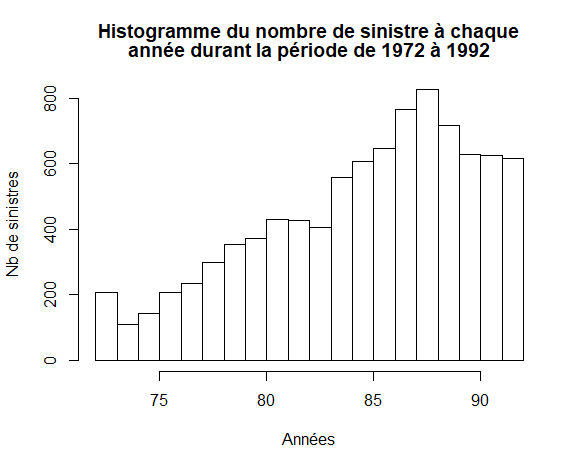
\includegraphics[scale=0.45]{Graphiques/HistFreqNorwegianfire} 
					\caption{} \label{HistFreqNorwegianfire}
				\end{subfigure}
				\begin{subfigure}[b]{0.4\textwidth}
					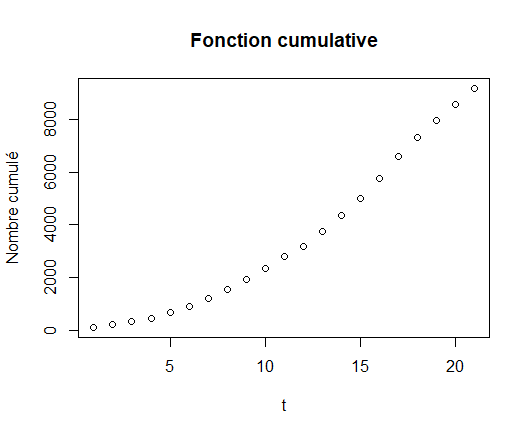
\includegraphics[scale=0.45]{Graphiques/Graph_Norwegianfire_FreqCumul} 
					\caption{} \label{Graph_Norwegianfire_FreqCumul}
				\end{subfigure}
				\renewcommand{\figurename}{Illustration}
				\caption{Analyse de la fréquence pour \texttt{norwegianfire}.}\label{Graph_Freq_NorvFire}
			\end{figure}
		
			Lorsque l'on regarde l'illustration \ref{HistFreqNorwegianfire}, on voit que l'intensité de la fréquence semble augmenter d'année en année. Cependant, entre les années 1986 et 1988, il s'est produit un événement qui a stoppé cet accroissement. En effet, en regardant l'analyse qui a été faite par la European Commission\footnote{\url{http://effis.jrc.ec.europa.eu/media/cms_page_media/40/Forest_fires_in_Europe_Middle_east_and_North_Africa_2016_final_pdf_JZU7HeL.pdf}}, aux page 36-38, on peut y voir que plusieurs mesures ont été prises par la Norvège afin de réduire le nombre d'incendies de forêt. De plus, en regardant l'illustration 33b de la dite analyse, on voit que le nombre de sinistres tend à redescendre. À noter que l'échelle de ce graphique est biaisée du fait que les méthodes statistiques avaient été changées. C'est pour cette raison que l'on voit une forte hausse en 2016; le biais a été corrigé à ce moment. En revanche, ce qui est intéressant de remarquer, c'est la tendance descendante jusqu'en 2015.\\
			
			Or, considérant que l'objectif de ce travail est de créer un modèle de prédiction du nombre de sinistres pour les années à venir, il faut que le processus utilisé soit représentatif des tendances futures. Pour cette raison, il est avisé de considérer un processus de Poisson homogène dont l'intensité serait la moyenne des trois dernières années de la base de données \texttt{norwegianfire}, soit 622 sinistres.
			
			\paragraph{Analyse de la sévérité:}
			Du point de vue de la sévérité, en regardant l'illustration \ref{Hist_SeverNorwegianFire}, on observe que les données extrêmes nuisent à la lecture de la distribution globale de la sévérité. L'illustration \ref{Hist_SevNorwegianFire2} permet, quant à lui, de remédier à ce problème. Ainsi, on observe que le logarithme des montants de sinistre semble suivre une loi exponentielle.
			
			\begin{figure}[H]
				\centering
				\begin{subfigure}[b]{0.3\textwidth}
					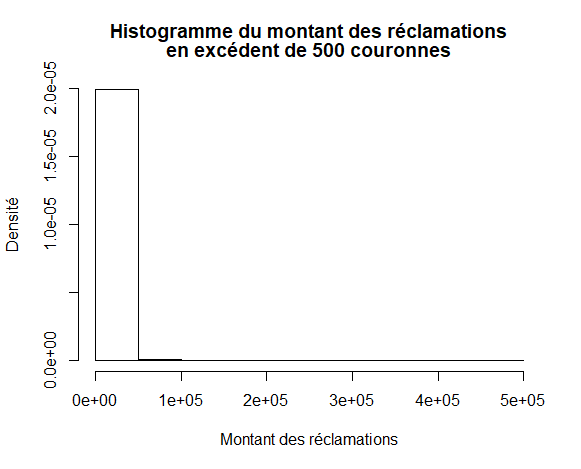
\includegraphics[scale=0.35]{Graphiques/Hist_SeverNorwegianFire} 
					\caption{} \label{Hist_SeverNorwegianFire}
				\end{subfigure}
				\begin{subfigure}[b]{0.3\textwidth}
					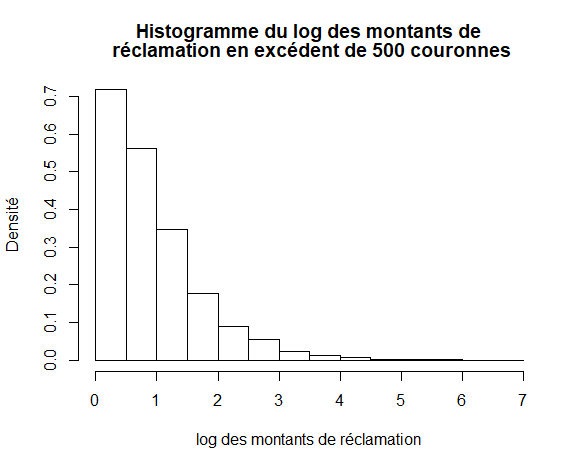
\includegraphics[scale=0.35]{Graphiques/Hist_SevNorwegianFire2}
					\caption{} \label{Hist_SevNorwegianFire2}
				\end{subfigure}
				\begin{subfigure}[b]{0.3\textwidth}
					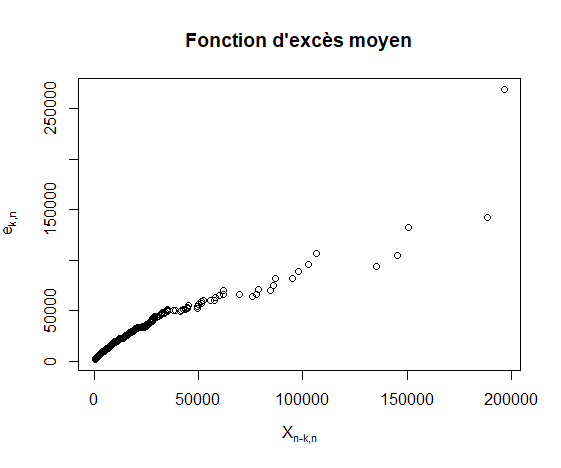
\includegraphics[scale=0.35]{Graphiques/Graph_Norwegianfire_MeanExcess} 
					\caption{} \label{Graph_Norwegianfire_MeanExcess}
				\end{subfigure}
				\renewcommand{\figurename}{Illustration}
				\caption{Analyse de la sévérité pour \texttt{norwegianfire}.} \label{Graph_Sev_NorvFire2}
			\end{figure}
			
			D'ailleurs, l'illustration \ref{QQplot_Pareto_NorweginaFIre} vient confirmer cette observation.
			
			\begin{figure}[H]
			\begin{center}
					\begin{subfigure}[H]{0.45\textwidth}
						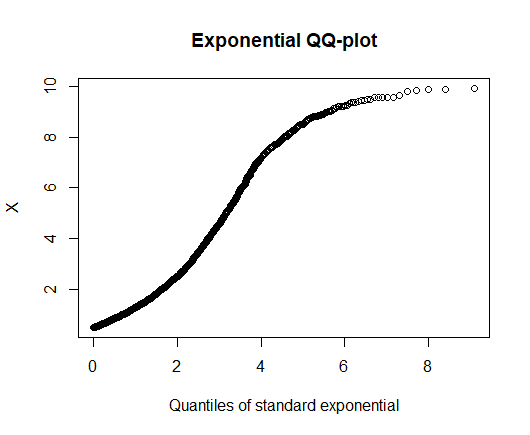
\includegraphics[scale=0.45]{Graphiques/QQplot_Exp_NorwegianFire}
						\caption{} \label{QQplot_Exp_NorwegianFire}
					\end{subfigure}
					\begin{subfigure}[H]{0.4\textwidth}
						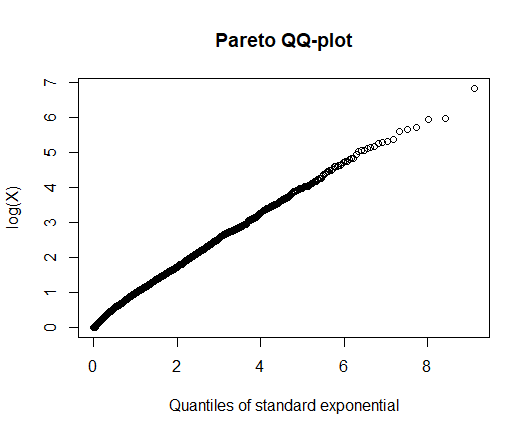
\includegraphics[scale=0.45]{Graphiques/QQplot_Pareto_NorweginaFIre}
						\caption{} \label{QQplot_Pareto_NorweginaFIre}
					\end{subfigure}
				\renewcommand{\figurename}{Illustration}
				\caption{\textit{QQplots} préliminaires pour \texttt{norwegianfire.}}
				\end{center}
			\textbf{Remarque:}\textit{Ces graphiques sont produits avec les commandes \texttt{R} provenant du \textit{package} \texttt{Reins: ExpQQ et ParetoQQ}.}
			\end{figure}
			En effet, l'illustration \ref{QQplot_Exp_NorwegianFire} montre le graphique des quantiles d'une loi exponentielle standard vis-à-vis des quantiles empiriques liés aux montants de sinistre tandis que l'illustration \ref{QQplot_Pareto_NorweginaFIre} compare les quantiles de la même loi exponentielle vis-à-vis du logarithme des données empiriques. 
			
			\begin{Proposition}\label{Propo_Pareto}
				Soit $X$, une variable aléatoire modélisant les montants de sinistre, \\si $\ln X \sim Exponentielle(\lambda)$, alors $X\sim Pareto(\lambda)$.
			\end{Proposition}
			
			\begin{proof}[Démonstration]
				Posons $Y=\ln X \sim Exp(\lambda)$. Alors, on a 
				$$
				\bar{F}_Y(y) = e^{-\lambda y} = e^{-\lambda \ln x} = x^{-\lambda} = \bar{F}_X(x),\: x\geq 1.
				$$
				On obtient alors la fonction de répartition d'une loi de Pareto de type 1 avec un paramètre de forme égal à $\lambda$ et le domaine débute à 1.
			\end{proof}

			Donc, on peut déduire de la proposition \ref{Propo_Pareto} qu'un modèle basé sur une loi de Pareto est un choix judicieux pour modéliser la sévérité de la base de données de la \texttt{norwegianfire}.\\
			
			Finalement, du point de vue des statistiques descriptives, le tableau \ref{Stats_Norwegianfire} résume les principaux points intéressants pour la sévérité des sinistres.
			
			\begin{table}[H]
				\begin{center}
				\begin{tabular}{ccccccc}
					Min.& $1^{er}$ Qu.	&	Médiane	&	Moyenne	&	$3^e$ Qu	&	Max.	&	écart type \\
					\hline
					500	&	700			&	1\,020	&	2\,217	&	1\,800		&	465\,400	&	7\,760
				\end{tabular}
				\renewcommand{\tablename}{Tableau}
				\caption{Statistiques descriptives de \texttt{norwegianfire}.}\label{Stats_Norwegianfire}
				\end{center}
			\end{table}
		
			Les statistiques du tableau \ref{Stats_Norwegianfire} sont utiles lors de l'établissement d'un point de départ dans l'algorithme d'estimation des paramètres avec la méthode du maximum de vraisemblance.
			
	\subsection{\texttt{secura}}
		Toujours dans le \textit{package} \texttt{Reins}, la base de données \texttt{secura} comporte des montants de perte en assurance automobile venant de plusieurs pays d'Europe pendant la période de 1988 à 2001. Ces montants sont en excédant de 1\,200\,000 euros et sont ajustées pour l'inflation.
		
		\paragraph{Analyse de la fréquence:}
		De façon similaire à l'analyse précédente, l'illustration \ref{Hist_freq_Secura} est un histogramme sur le nombre annuel de sinistres dans la période de 1988 à 2001 et l'illustration \ref{Graph_Secura_FreqCumul} présente la fonction de répartition empirique de ce dénombrement.
		
		\begin{figure}[H]
			\begin{center}
				\begin{subfigure}[b]{0.45\textwidth}
					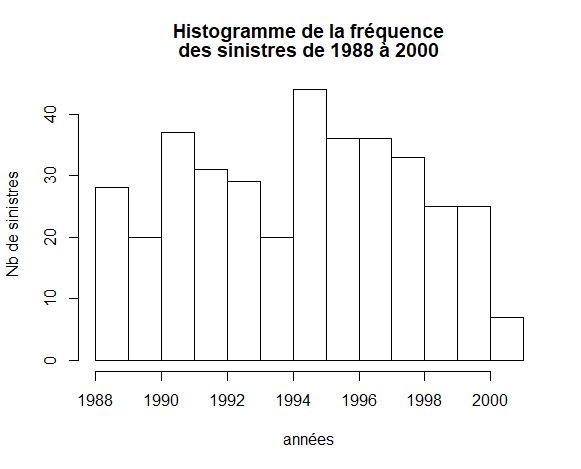
\includegraphics[scale=0.45]{Graphiques/Hist_freq_Secura} 
					\caption{} \label{Hist_freq_Secura}
				\end{subfigure}
				\begin{subfigure}[b]{0.4\textwidth}
					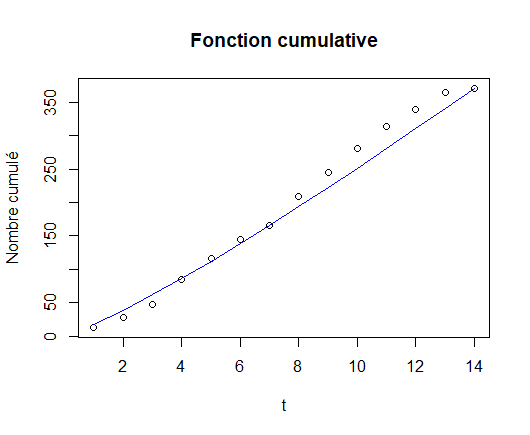
\includegraphics[scale=0.45]{Graphiques/Graph_Secura_FreqCumul} 
					\caption{} \label{Graph_Secura_FreqCumul}
				\end{subfigure}
			\renewcommand{\figurename}{Illustration}
			\caption{Analyse de la fréquence pour \texttt{secura}.}\label{Graph_freq_Secura}
			\end{center}
		\end{figure}
	
		À la lecture de l'illustration \ref{Hist_freq_Secura}, on voit que la fréquence des sinistres semblent avoir une tendance cyclique sur 4 ans. Cependant, selon le contexte, cela est très peu probable puisque il est illogique de penser que le nombre d'accidents diminuerait à tous les quatre ans pour ensuite remonter d'un coup à un niveau plus élevé. Par contre, suite à la recherche de données complémentaires sur l'internet, aucune information ne nous permet de contredire ces résultats. Pour cette raison, on ne peut assumer que ces informations sont fausses \textit{a posteriori} et elles doivent être considérer comme tel dans l'analyse de la fréquence.\\
		
		À ce moment, il est approprié de tester un processus de Poisson non-homogène avec une intensité périodique afin d'étudier ce comportement. Par ailleurs, en regardant l'illustration \ref{Graph_Secura_FreqCumul}, on voit que cette périodicité n'est peut être pas significative puisque les écarts entre les points et la droite qui est tracée ne sont pas très grands. Afin de comparer ces deux modèles, il est nécessaire de procéder au test du ratio de maximum de vraisemblance pour valider s'il y a réellement un gain à avoir un modèle plus complexe par rapport à un processus de Poisson homogène.
		
		\paragraph{Analyse de la sévérité:}
		Au niveau de l'analyse de la sévérité, en regardant l'illustration \ref{Hist_Severite_Secura}, une loi de forme exponentielle semble, \textit{a priori}, bien modéliser le corps de la distribution. 
		
		\begin{figure}[H]
		\begin{center}
		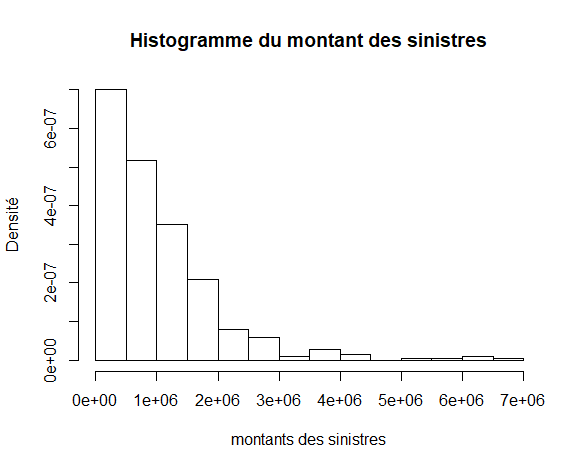
\includegraphics[scale=0.45]{Graphiques/Hist_Severite_Secura} 
		\renewcommand{\figurename}{Illustration}
		\caption{Analyse de la sévérité pour \texttt{secura}.} \label{Hist_Severite_Secura}
		\end{center}
		\end{figure}
		
		L'illustration \ref{QQPlot_Expo_Secura} permet, quant à lui, de confirmer cette hypothèse.
		
		\begin{figure}[H]
			\begin{center}
				\begin{subfigure}[b]{0.45\textwidth}
					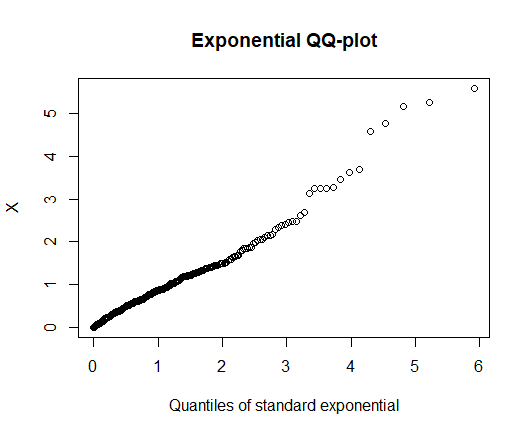
\includegraphics[scale=0.43]{Graphiques/QQPlot_Expo_Secura} 
					\caption{} \label{QQPlot_Expo_Secura}
				\end{subfigure}
				\begin{subfigure}[b]{0.4\textwidth}
					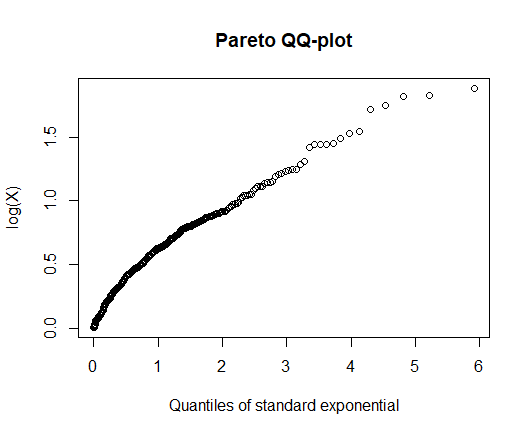
\includegraphics[scale=0.43]{Graphiques/QQplot_Pareto_Secura} 
					\caption{} \label{QQplot_Pareto_Secura}
				\end{subfigure}
				\renewcommand{\figurename}{Illustration}
				\caption{\textit{QQplots} préliminaires pour \texttt{secura}.}
			\end{center}
		\end{figure}
		
		En revanche, en regardant l'illustration \ref{Graph_Secura_MeanExcess}, on voit de façon plus détaillé quelles lois pourraient être utilisées.\\
		
		\begin{figure}[H]
			\begin{center}
			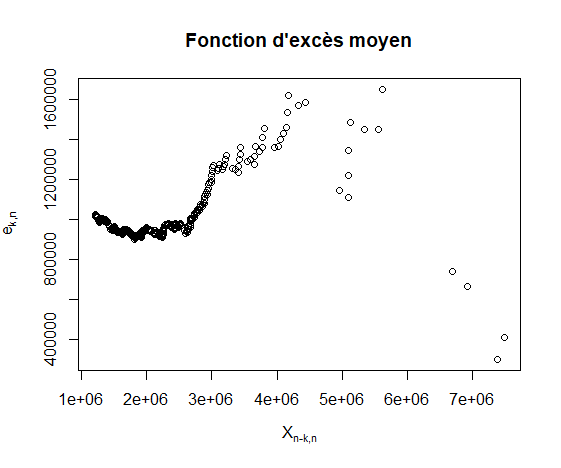
\includegraphics[scale=0.45]{Graphiques/Graph_Secura_MeanExcess} 
			\renewcommand{\figurename}{Illustration}
			\caption{Fonction d'excès moyen pour \texttt{secura}.} \label{Graph_Secura_MeanExcess}
			\end{center}
		\end{figure}
		
		En effet, \cite{Embrechts1994}(p.11-14) font  une analyse de distribution se basant sur la fonction d'excès moyen. Les résultats de cette analyse sont résumés sur l'illustration \ref{Interpretation_Graph_ExcesMoyens}.
		
		\begin{figure}[H]
			\begin{center}
			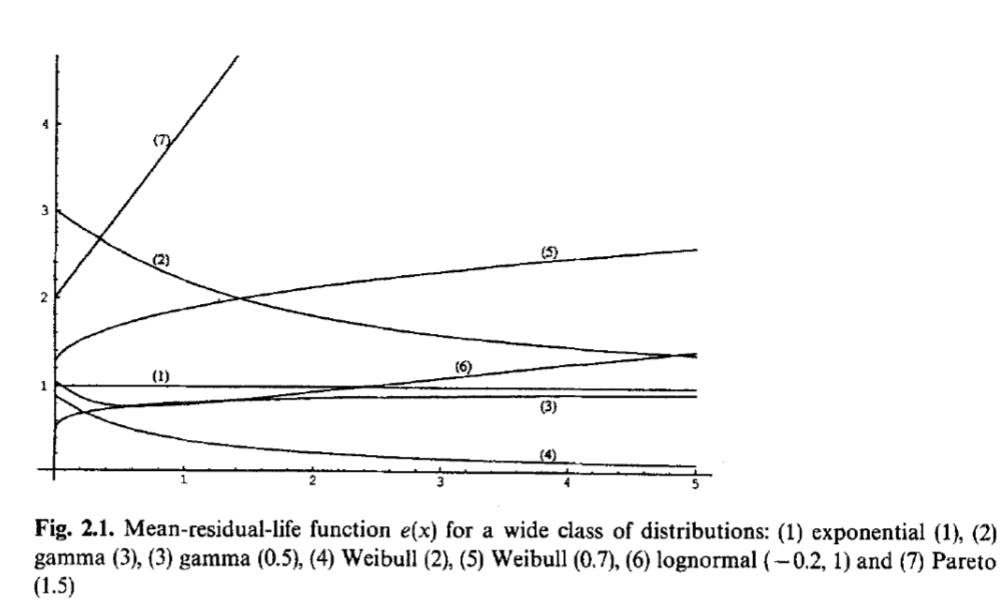
\includegraphics[scale=0.45]{Graphiques/Interpretation_Graph_ExcesMoyens} 
			\renewcommand{\figurename}{Illustration}
			\caption{Embrechts et Schmidli: Détermination de la loi de sévérité en fonction de la fonction d'excès moyen.} \label{Interpretation_Graph_ExcesMoyens}
			\end{center}
		\end{figure}
		
		Ainsi, en observant, le graphique d'excès moyen, nous sommes en mesure de faire une analyse approfondie afin de déterminer de façon analytique quelles lois pourraient être utilisées. De plus,  advenant de devoir faire des raccordements de lois, cet indicateur peut aider, en théorie, à déterminer les valeurs de $X$ où il faut appliquer les points de raccordement.\\
		
		De cette façon, en regardant à nouveau l'illustration \ref{Graph_Secura_MeanExcess}, on peut voir que les deux lois pouvant modéliser le mieux le début de la distribution seraient la loi gamma ou possiblement la loi de Weibull. Puis, un premier raccordement serait fait aux alentours de $2\,900\,000$ \euro. À cette valeur, un raccordement approprié serait fait avec une loi de Pareto afin de bien représenter les valeurs extrêmes. Cependant, la nature des points qui suivent n'est pas claire à ce stade-ci de l'analyse.\\
		
		Néanmoins, plusieurs modèles doivent être testés afin de valider les hypothèses soulevées grâce à la découverte de \cite{Embrechts1994} et pour optimiser la vraisemblance du modèle.\\
						
		Finalement, les statistiques descriptives de la base de données sont présentées dans le tableau \ref{Stats_Secura}.
				
		\begin{table}[H]
			\begin{center}
				\begin{tabular}{ccccccc}
					Min.& $1^{er}$ Qu.	&	Médiane	&	Moyenne	&	$3^e$ Qu	&	Max.	&	écart type \\
					\hline
					1\,208\,000 & 1\,573\,000 & 1\,944\,000 & 2\,231\,000 & 2\,609\,000 & 7\,899\,000 	&	1\,011\,218
				\end{tabular}
				\renewcommand{\tablename}{Tableau}
				\caption{Statistiques descriptives de \texttt{secura}.}\label{Stats_Secura}
			\end{center}
		\end{table}
	
	En regardant ce tableau, on voit que la valeur minimale de l'échantillon est de $1\,208\,000$ \euro. Malgré cette information, pour le présent travail, il est assumé que les données ont bien été tronquées à $1\,200\,000$ \euro\;afin d'être cohérent avec l'analyse descriptive ci-haut.
	
	\subsection{\texttt{danish}}
		La dernière base de données, \texttt{danish}, se trouve dans le \textit{package} \texttt{R CASdataset} avec la commande \texttt{data(danishuni)}. Elle est aussi disponible au lien suivant: \url{http://www.ma.hw.ac.uk/~mcneil/data.html}. Elle a été compilée à la Copenhagen Reinsurance et comprend 2\,167 pertes liées à des incendies au cours de la période de 1980 à 1990. Elle a été ajustée pour inflation et les valeurs sont exprimées en millions de couronnes danoises.\\
		
		Par ailleurs, ce qui distingue cette base de données des deux autres, c'est qu'elle présente les sinistres à chaque jour. Il est donc possible d'avoir une analyse de la fréquence plus approfondie. Malheureusement, pour pouvoir tester un processus de renouvellement, il aurait fallu qu'il n'y ait pas plus d'un événement par jour ou que la périodicité soit exprimé en termes d'heures. Or, comme ce n'est pas le cas, il n'est pas possible de modéliser les temps inter-sinistres adéquatement.
		
		\paragraph{Analyse de la fréquence:}
		Comme pour les deux autres bases de données, l'analyse préliminaire débute avec l'histogramme \ref{Hist_Danish_Frequence} qui présente le nombre de sinistres dans la période de 1980 à 1990, sur une base quotidienne, puis le graphique \ref{Graph_Danish_FreqCumul} qui présente la fonction de répartition  empirique de ce dénombrement.
		
		\begin{figure}[H]
			\begin{center}
				\begin{subfigure}[b]{0.52\textwidth}
					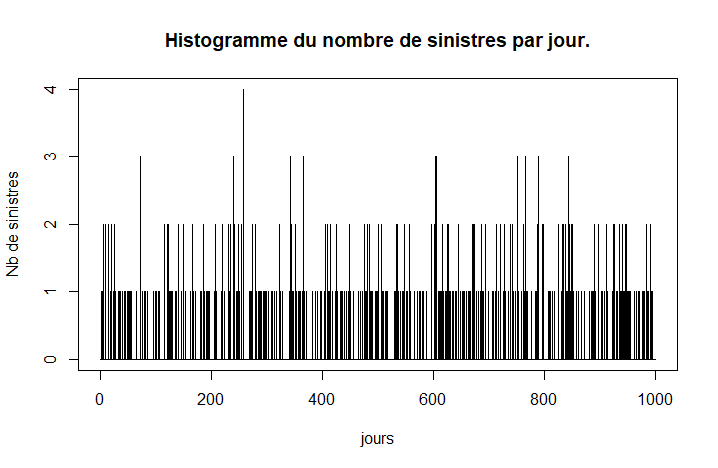
\includegraphics[scale=0.5]{Graphiques/Hist_Danish_Frequence} 
					\caption{} \label{Hist_Danish_Frequence}
				\end{subfigure}
			\begin{subfigure}[b]{0.42\textwidth}
				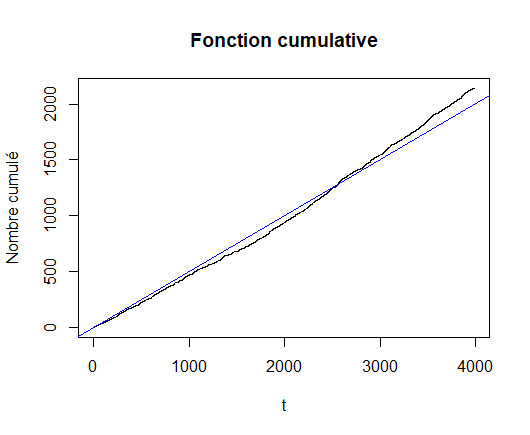
\includegraphics[scale=0.5]{Graphiques/Graph_Danish_FreqCumul} 
				\caption{} \label{Graph_Danish_FreqCumul}
			\end{subfigure}
			\renewcommand{\figurename}{Illustration}
			\caption{Analyse de la fréquence pour \texttt{danish}.}\label{Graph_Freq_Danish}
			\end{center}
		\end{figure}
		
		L'illustration \ref{Graph_Danish_FreqCumul} montre qu'il y a une très légère hausse de l'intensité au fil du temps.\\
		
		Cependant, l'illustration \ref{Graph_CompLimit_PoissHomo} peut laisser croire qu'il s'agit d'un processus de Poisson homogène puisque l'on peut y observer le comportement limite d'un processus de Poisson dont l'intervalle de temps tend vers l'infini.
		
		\begin{figure}[H]
			\begin{center}
			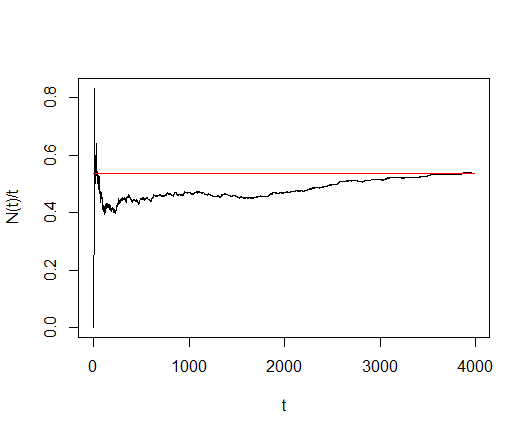
\includegraphics[scale=0.5]{Graphiques/Graph_CompLimit_PoissHomo} 
			\end{center}
			\renewcommand{\figurename}{Illustration}
			\caption{Comportement limite d'un Processus de Poisson.} Lorsque l'intervalle de temps(t) sur lequel un Processus de Poisson est étudié est grand, le nombre de sinistres divisé par l'intervalle de temps sur lesquels ces sinistres ont été observés tend vers le taux d'intensité du Processus.(\cite{Mikosch_PoissProcess2009}, p.56-60).\label{Graph_CompLimit_PoissHomo} 
		\end{figure}
	
		Comme pour la base de données \texttt{secura}, le test du ratio de vraisemblance permet de déterminer si l'augmentation est significative ou si un modèle de Poisson homogène capture réellement le comportement de ces données.
		
		\paragraph{Analyse de la sévérité:}
		Pour ce qui est de la sévérité, en regardant les graphiques \ref{Hist_Danish_Severite} et \ref{Hist_Danish_LogSeverite}, un comportement similaire à celui de la base de données \texttt{norwegianfire} est observable. En effet, le logarithme des montants de sinistre semble suivre une loi exponentielle. L'utilisation d'un modèle basé sur la loi de Pareto semble donc aussi adéquat.
		
		\begin{figure}[H]
			\begin{center}
			\begin{subfigure}[b]{0.3\textwidth}
				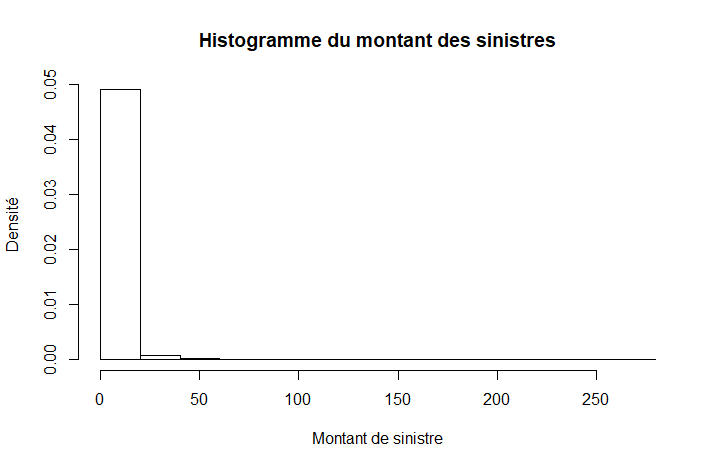
\includegraphics[scale=0.35]{Graphiques/Hist_Danish_Severite} 
				\caption{} \label{Hist_Danish_Severite}
			\end{subfigure}
			\begin{subfigure}[b]{0.3\textwidth}
				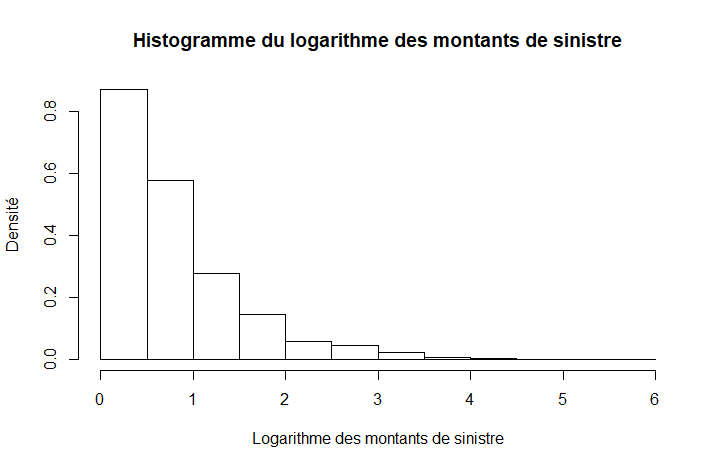
\includegraphics[scale=0.35]{Graphiques/Hist_Danish_LogSeverite} 
				\caption{} \label{Hist_Danish_LogSeverite}
			\end{subfigure}
			\begin{subfigure}[b]{0.3\textwidth}
				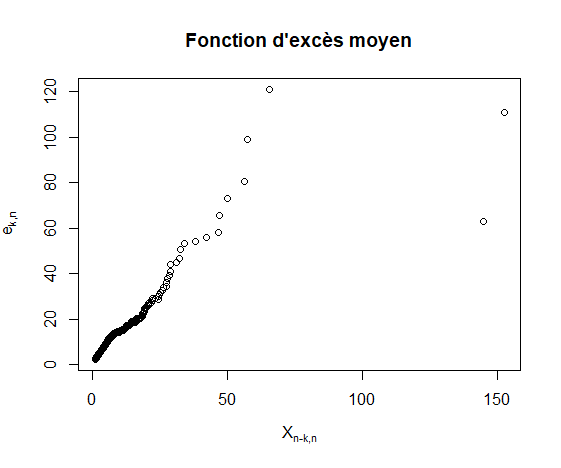
\includegraphics[scale=0.35]{Graphiques/Graph_Danish_MeanExcess} 
				\caption{} \label{Graph_Danish_MeanExcess}
			\end{subfigure}
			\renewcommand{\figurename}{Illustration}
			\caption{Analyse de la sévérité pour \texttt{danish}.}\label{Hist_Danish}
			\end{center}
		\end{figure}
		
		De plus, l'illustration \ref{QQplot_Pareto_Danish} vient confirmer cette observation.
		
		\begin{figure}[H]
			\begin{center}
				\begin{subfigure}[b]{0.5\textwidth}
					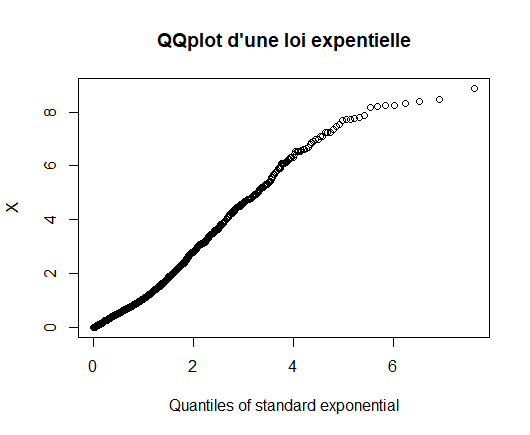
\includegraphics[scale=0.45]{Graphiques/QQplot_Exp_Danish} 
					\caption{Fréquence} \label{QQplot_Exp_Danish}
				\end{subfigure}
				\begin{subfigure}[b]{0.4\textwidth}
					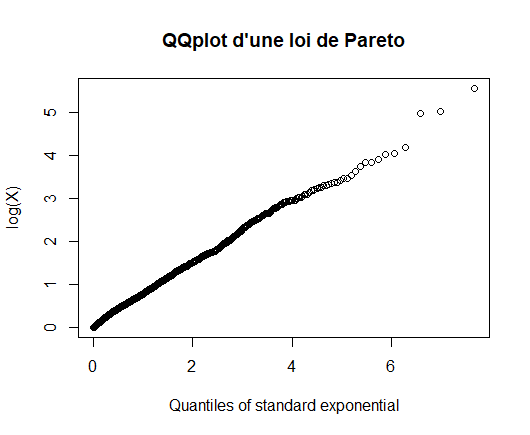
\includegraphics[scale=0.45]{Graphiques/QQplot_Pareto_Danish} 
					\caption{Sévérité} \label{QQplot_Pareto_Danish}
				\end{subfigure}
				\renewcommand{\figurename}{Illustration}
				\caption{\textit{QQplots} préliminaires pour \texttt{danish}.}
			\end{center}
		\end{figure}
		
		En regardant le tableau \ref{Stats_Danish}, on voit que la valeur minimale est d'un million de couronnes danoises. Donc, il faut conditionner sur cette valeur où se trouve la troncature.
		
		\begin{table}[H]
			\begin{center}
				\begin{tabular}{ccccccc}
					Min.& $1^{er}$ Qu.	&	Médiane	&	Moyenne	&	$3^e$ Qu	&	Max.	&	écart type \\
					\hline
					1,000  & 1,321 &  1,778 &  3,385 &  2,967 & 263,300  	&	8,507
				\end{tabular}
				\renewcommand{\tablename}{Tableau}
				\caption{Statistiques descriptives de \texttt{danish}.}\label{Stats_Danish}
			\end{center}
		\end{table}		
		 % Contient la description des bases de données avec une analyse préliminaire des données
	\section{Analyse de la fréquence}\label{Section_Frequence}
	Lors de l'analyse du capital à investir pour une compagnie de réassurance, il va de soit que le dénombrement des sinistres à une importance toute aussi grande que pour la modélisation de la sévérité selon la \textit{théorie des modèles collectifs du risque}. \\
	
	Afin d'analyser cette composante, \cite{Parodi2015_Pricing_in_GenIns}(p.187-206) suggère une approche selon les lois de dénombrement classiques telles que la loi binomiale, binomiale négative et la loi de Poisson. Cependant, cette approche ne tient pas compte des tendances qu'il peut y avoir à travers le temps.\\
	
	Ainsi, afin de pouvoir étudier l'évolution du dénombrement des sinistres dans le temps, il faut utiliser les processus stochastiques. Dans cette perspective, \cite{Mikosch_PoissProcess2009}(p.7-9) recommande d'utiliser les processus de Poisson.\\
	
	Dans cette section, les processus de Poisson homogènes et non homogènes sont donc testés afin de modéliser le dénombrement des sinistres d'une année à l'autre.
	
	\begin{Definition}
		Soit $\{ N(t)\in \mathbb{N};t>0 \} $, un processus de comptage dont les accroissements sur l'intervalle de temps $(s,t]$ sont définis par $\{ N(t)-N(s),\:t>s\}$. Si on définit que les temps inter-sinistres suivent une loi exponentielle, ce processus de comptage obéit à une loi de Poisson dont la fonction de masse de probabilités est définie par
		\begin{align}
		P\left[N\left(t\right)-N\left(s \right) = x \right] = \frac{\left[\Lambda(t) - \Lambda(s)\right]^x e^{-\left[\Lambda(t) - \Lambda(s)\right]}}{x!}  \label{ProcessusPoisson}
		\end{align}
		et l'espérance des accroissements, $\Lambda \left( t\right) -\Lambda \left( s\right) $, correspond à 
		\begin{align}
		E[N(t)-N(s)] = \Lambda(t) - \Lambda(s) = \int_{s}^{t} \lambda(u)\textrm{d}u \;  ,\ 0<s<t, \label{Esp_Accroissements}
		\end{align}
		où $\lambda$ correspond au taux d'intensité du processus. 
	\end{Definition}

	Dans le présent travail, afin d'estimer les paramètres des processus de Poisson, la méthode du maximum de vraisemblance est utilisée puisque celle-ci comporte des propriétés théoriques favorables (voir \cite{Edward_MaximumLikelyhood1988}, p.347-362). \\
	
	\subsection{Processus de Poisson homogène}
		 Pour débuter, le processus de Poisson homogène possède un taux d'intensité constant. Ainsi, afin d'en estimer son paramètre, il suffit de maximiser la fonction de vraisemblance tel qu'elle est définit par
		\begin{align}
			\mathcal{L}\left(\lambda\right)  
			&= \prod_{i=1}^{n} f_{N(t)_i} \left( x_i, \lambda, t \right) \nonumber\\
			&= \prod_{i=1}^{n} \frac{ \left( \lambda t \right)^{x_i} e^{-\lambda t} }{x_i!}, \label{Fct_Vraiss_PoissHomo}
		\end{align}
		où $n$ correspond au nombre d'observations de la base de données.\\
		Cependant, il est plus aisé de maximiser la log-vraisemblance qui est
		\begin{align}
			l \left(\lambda \right)  
			&= \sum_{i=1}^{n}  \left( x_i \ln\left(\lambda t\right)-\lambda t - \ln \left(x_i!\right)  \right) \nonumber\\
			&= n \bar{x} \ln \left( \lambda t \right) - n\lambda t - \sum_{i=1}^{n}\ln \left(x_i!\right). \label{Fct_logVraiss_PoissHomo}
		\end{align}
		En dérivant \ref{Fct_logVraiss_PoissHomo} en fonction de $\lambda$ et en égalisant le résultat à zéro, on obtient $\hat{\lambda}$, l'expression de l'estimateur du maximum de vraisemblance de $\lambda$, soit
		$$	\hat{\lambda} = \bar{x}/t. $$
		
		Ainsi, selon la méthode du maximum de vraisemblance, le meilleur estimateur du paramètre $\lambda$ d'une loi de Poisson homogène est la moyenne du nombre de sinistre dans l'intervalle de temps $t$, divisé par ce dernier.
		
	\subsection{Processus de Poisson non homogène}
		Lorsque l'intensité d'un processus de Poisson n'est pas constant dans le temps, il survient que les accroissements ne sont pas stationnaires. Cela signifie que si ce processus débute au temps 0, il n'aura pas la même intensité que s'il débute au temps $t$, pour $t>0$. On obtient alors des processus légèrement plus complexes à modéliser. \\
		
		Parmi l'infinité de modèles qui existent pour capturer ces tendances au fil du temps, quelques-un sont proposés par \cite{Kuhl_PoissonNonHomo_Trends_1997}. Cependant, parmi ceux-ci, certains donnent des résultats douteux sur le long terme. Ce qui amène à considérer qu'il faut faire attention à ne pas faire du surapprentissage statistique. C'est à dire que le modèle n'est bon que pour modéliser les données qui ont servi à l'entraîner. Pour cette raison, les modèles trop complexes perdent du pouvoir prédictif.\\
		
		Pour ce travail, les modèles ont été sélectionnés parmi ceux proposées dans \cite{TheorieDuRisque2018_MarceauEtCossette}(p.231). Ainsi, la fonction linéaire, la fonction de puissance et la fonction périodique avec effet saisonnier sont les modèles d'intensité retenus.
		
		\subsubsection{Intensité linéaire}
			Le processus de Poisson avec intensité linéaire est celui qui permet de modéliser une augmentation de l'intensité qui est constant dans le temps comme dans le cas des bases de données \texttt{norwegianfire} (graphique \ref{Graph_Norwegianfire_FreqCumul}) et \texttt{danish} (graphique \ref{Graph_Danish_FreqCumul}).
			\begin{Proposition}
			 	Soit $\lambda(u) = a+bu \ , \; a>0,\,b\geq 0, u>0$. Alors, on obtient 
				\begin{align}
				\Lambda(t+1) - \Lambda(t) = a+\frac{b(2t+1)}{2}. \label{Intensite_lineaire}
				\end{align}
			\end{Proposition}
			\textit{Preuve:} L'expression en \ref{Intensite_lineaire} est obtenue directement en appliquant \ref{Esp_Accroissements}.\\
			
	 		Il s'ensuit que la fonction de vraisemblance est définie par 
		 	 	\begin{align}
		 	 		\mathcal{L}\left( a,b \right) = \prod_{i=1}^{n} \frac{ \left( a+\frac{b(2t+1)}{2} \right)^{x_i} e^{-(a+\frac{b(2t+1)}{2})} }{x_i}. \label{Vrais_Poiss_Homo}
		 	 	\end{align}
				
			Puis la fonction de log-vraisemblance est
			\begin{align}	
				l\left(a,b\right) 
				&= \sum_{i=1}^{n} \left( x_i \ln \left( a+\frac{b(2t+1)}{2} \right) -a-\frac{b(2t+1)}{2} -\ln x_i   \right) \nonumber \\
				&=n\bar{x}\ln \left( a+\frac{b(2t+1)}{2} \right) - na - \frac{nb(2t+1)}{2} -\sum_{i=1}^{n}\ln x_i. \label{Log-Vrais_Poiss_Homo}
			\end{align}
			
			À ce stade, le système d'équations qui découle de \ref{Log-Vrais_Poiss_Homo} peut être résolu numériquement.\\
			
			Dans son mémoire de maîtrise, \cite{Drazek_PoissProcess2013}(p.32-33) a développé un algorithme pour trouver les paramètres de processus de Poisson. Dans son ouvrage, il minimise la log-vraisemblance négative puisque la majorité des commandes d'optimisation numériques sont programmées pour minimiser des fonctions. \\
			
			Le code \texttt{R} qui a été utilisé pour estimer les paramètres des processus de Poisson non homogène avec intensité linéaire est présenté dans le code informatique \ref{Code_ProcessusPoisson_homo}.
			\begin{Code} \label{Code_ProcessusPoisson_homo}
				\begin{verbatim} 
				
				neg_log_vrais <- function(para){
				-sum( log( dpois(data, para[1] + para[2] * (2*t+1)/2)))
				}
				
				mle <- constrOptim(c(0.05, 0), neg_log_vrais, grad = NULL, 
				ui = c(1,0), ci = 0,outer.eps = .Machine$double.eps)
				\end{verbatim}
			\end{Code}
			Afin de trouver des valeurs de départ pour cet outil d'optimisation, une façon appropriée est d'utiliser la méthode des moments qui est proposé dans \cite{LossModels_Klugman2012}(p.253-255).\\
			
			À noter que les fonctions \texttt{optim} et \texttt{constrOptim} donnent des résultats plus précis lorsque les valeurs de départs sont proches du résultat attendu.
			En changeant ces paramètres initiaux, les deux fonctions retourneront des résultats qui peuvent beaucoup fluctuer.
					
		\subsubsection{L'intensité est une fonction de puissance}
			Advenant le cas où l'augmentation de l'intensité se fait de façon plus prononcée qu'avec un modèle linéaire, il est possible d'utiliser une fonction de puissance. Dans le cas présent, cette fonction s'inspire de la loi de Weibull.
			
			\begin{Proposition}
				Soit $\lambda(u) = (\beta u)^\tau \ , \; \beta>0,\,\tau>0, u>0.$ Alors on a 
				\begin{align}
				\Lambda(t+1) - \Lambda(t) = \frac{\beta^\tau}{\tau+1}((t+1)^{\tau+1}-t^{\tau+1}) \label{Intens_Poiss_Puissance}.
				\end{align}
			\end{Proposition}
			\textit{Preuve:} L'expression en \ref{Intens_Poiss_Puissance} est obtenue directement en appliquant \ref{Esp_Accroissements}.\\
			
			Puis, la fonction de vraisemblance est définie par
			\begin{align}
			\mathcal{L}\left( x,\beta,\tau,t \right) 
			= \prod_{i=1}^{n} \frac{ \left( \frac{\beta^\tau}{\tau+1}((t+1)^{\tau+1}-t^{\tau+1}) \right)^{x_i} e^{-(\frac{\beta^\tau}{\tau+1}((t+1)^{\tau+1}-t^{\tau+1}))} }{x_i}.\label{Vrais_Poiss_Puissance}
			\end{align}
			
			Dans ce cas-ci, pour trouver les estimateurs des paramètres, le plus simple est d'utiliser la méthode algorithmique de la même façon que pour le cas précédent.\\
			
			Par ailleurs, afin de simplifier l'algorithme, il est possible de réécrire l'intensité cumulée sous la forme
			
			\begin{align}
				\Lambda(t+1) - \Lambda(t) 
				&= \frac{\beta^\tau}{\tau+1}((t+1)^{\tau+1}-t^{\tau+1}) \nonumber\\
				&= \beta^* ((t+1)^{\tau^*} - t^{\tau^*}), t>0, \label{Intensite_Fonctio_Puissance}
			\end{align} 
			
			où $\beta^*=\beta^\tau$ et $\tau^*=\tau+1$.\\
			
			L'algorithme \texttt{R} permettant de procéder à cette optimisation est reproduit dans le code informatique \ref{Code_Parametres_PoissPuissance}.
			
			\begin{Code}\label{Code_Parametres_PoissPuissance}
			\begin{verbatim}
			
				intensite <- function(t,para){
				(para[1] * t)^para[2]
				}
				
				neg_log_vrais <- function(para){
				-sum( log( dpois(data, intensite(t+1,para) - intensite(t, para))))
				}
				
				mle_nonhomo_wei <- constrOptim(c(1, 1), neg_log_vrais, grad = NULL, 
				ui = c(1,0), ci = 0,outer.eps = .Machine$double.eps)
			\end{verbatim}
		\end{Code}
			
		\subsubsection{Intensité périodique}
			Finalement, le modèle d'intensité périodique permet de capturer une tendance cyclique comme dans le cas de \texttt{secura} avec le graphique \ref{Graph_Secura_FreqCumul}.
			\begin{Proposition}\label{Intens_Periodique}
			Soit $\lambda(u) = a+b \cos\left(\frac{2\pi u}{c}\right) \ , \; a>0,\,b \in \left[0,a\right],\,c>0, u>0. $ Alors, on a\\
			\begin{align*} 
				\Lambda(t+1) - \Lambda(t) = a-\frac{bc}{2\pi}\left[\sin\left(\frac{2\pi(t+1)}{c}\right)-\sin\left(\frac{2\pi(t)}{c}\right)\right] .
			\end{align*}
			\end{Proposition}
			\textit{Preuve:} Il suffit d'appliquer \ref{Esp_Accroissements}.\\
			
			Dans la proposition \ref{Intens_Periodique} on interprète $a$ comme étant une tendance cyclique (par exemple annuelle), $b$ comme étant l'intensité des cycles et $c$ comme étant la durée d'un cycle complet. \\
			
			Il s'ensuit que la fonction de vraisemblance est
			\begin{align*}
			\mathcal{L}\left( x,a,b,t \right) 
				&= \prod_{i=1}^{n} \frac{ \left(  a-\frac{bc}{2\pi}\left[\sin\left(\frac{2\pi(t+1)}{c}\right)-\sin\left(\frac{2\pi(t)}{c}\right)\right]  \right)^{x_i} 		e^{-\left(a-\frac{bc}{2\pi}\left[\sin\left(\frac{2\pi(t+1)}{c}\right)-\sin\left(\frac{2\pi(t)}{c}\right)\right] \right)} }{x_i}.\\
			\end{align*}
			
			Encore ici, le plus simple est d'utiliser la méthode algorithmique décrite dans le code informatique \ref{Code_Parametres_PoissSaisonnier}.
			
			\begin{Code} \label{Code_Parametres_PoissSaisonnier}
			\begin{verbatim}	
			
			intensite_cos <- function(t,para){
			para[1] * t - para[2] * sin(2 *pi *t /para[3])
			}
			
			neg_log_vrais <- function(para){
			-sum( log( dpois(data, intensite_cos(t,para) - intensite_cos(t-1,para) )))
			}
			
			mle_nonhomo_cos <- constrOptim(c(20,10,8), neg_log_vrais, grad = NULL, 
			ui = diag(3), ci = c(0,0,0),outer.eps = .Machine$double.eps)
			\end{verbatim}
			\end{Code}
	\section{Analyse de la sévérité de façon univariée}\label{Section_Severite}
	Comme il est expliqué dans \cite{Parodi2015_Pricing_in_GenIns}(p.225) et dans \cite{TheorieDuRisque2018_MarceauEtCossette}(p.79), les lois de sévérités qui sont généralement à privilégier en contexte d'assurance sont des lois continues avec un support sur les réels positifs et possédants une asymétrie positive. De plus, comme Parodi l'explique dans son ouvrage, les lois les plus simples (moins de paramètres) sont souvent les meilleures candidates pour la modélisation. En effet, selon la théorie de l'apprentissage statistique, un modèle plus complexe que nécessaire offre un faible pouvoir de prédiction. Par ailleurs, des tests de comparaison tels que le critère d'information d'Akaike (AIC) ou le critère d'information bayésien de Schwartz (BIC) pénalisent le nombre de paramètres. Pour cette raison il faut vérifier l'adéquation des modèles univariés avant de regarder les modèles avec raccordement.\\
	
	Pour débuter l'analyse univariée, il serait intéressant de regarder plus en détail le comportement de la fonction d'excès moyen expliqué dans l'illustration \ref{Graph_MeanExcess} pour identifié les lois à utiliser. Ainsi, dans l'illustration \ref{Graph_MeanExcess}, on voit les principales lois utilisées pour ce travail.
	
	\begin{figure}[H]
		\begin{center}
		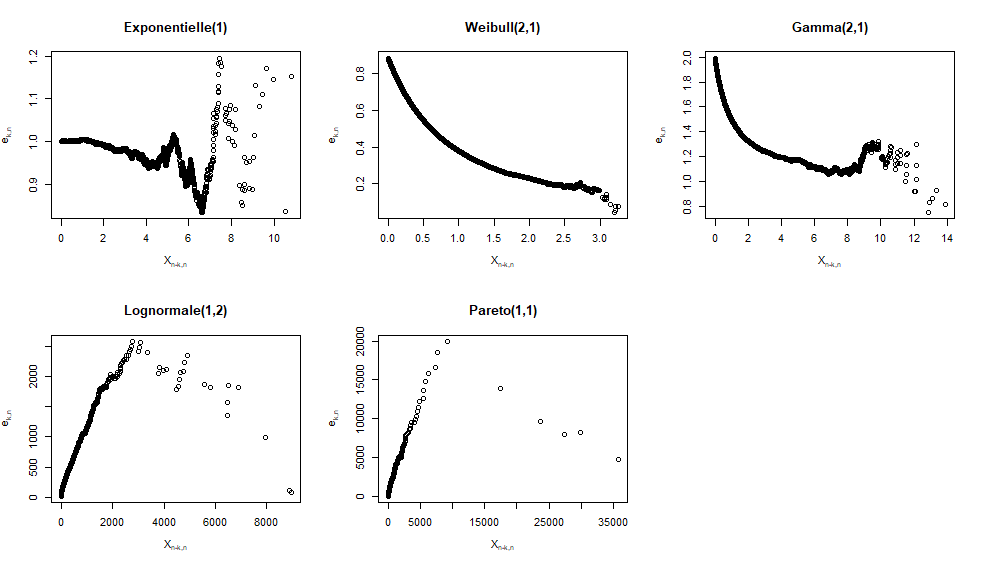
\includegraphics[scale=0.7]{Graphiques/Graph_MeanExcess} 
		\renewcommand{\figurename}{Illustration}
		\caption{Simulation du comportements de la fonction d'excès moyen selon le type de loi.} \label{Graph_MeanExcess}
	\end{center}
	\end{figure}

	Le premier constat de cette analyse graphique est qu'il ne faut pas nécessairement se fier sur les valeurs extrêmes de cette fonction pour définir des raccordement. En effet, ces graphiques ont été générés par simulation avec le code informatique \ref{Code_MeanExcess_Graphs}. Bien qu'il s'agisse de simulations de lois paramétriques, des valeurs aberrantes apparaissent dans la queue de la fonction d'excès moyen. \\
	
	\begin{Code}\label{Code_MeanExcess_Graphs}
		\begin{verbatim}
		
		set.seed(20181128)
		m <- 10^5
		par(mfrow=c(2,3))  
		MeanExcess(rexp(m),main = "Exponentielle(1)")
		MeanExcess(rweibull(m,2,1),main = "Weibull(2,1)")
		MeanExcess(rgamma(m,2,1),main = "Gamma(2,1)") 
		MeanExcess(rlnorm(m,1,2),main = "Lognormale(1,2)")
		MeanExcess(rpareto(m,1,1),main = "Pareto(1,1)")
		\end{verbatim}
	\end{Code}

	Le meilleur exemple de ce constat se produit avec la loi exponentielle. Comme celle-ci possède la propriété sans mémoire, la fonction d'excès moyen devrait être une constante. C'est à dire qu'on devrait observer une ligne droite. Cependant, comme on le voit dans l'illustration \ref{Graph_MeanExcess}, à partir du moment où on aperçoit des soubresauts dans la courbe, la fonction d'excès moyen ne semble plus être un bon indicateur de la loi.\\
	
	La raison qui explique ce phénomène est que l'estimateur empirique de la fonction d'excédent est une moyenne. Lorsque le nombre d'observations constituant cette moyenne diminue, la variabilité de l'estimateur augmente significativement. \\
	
	Pour aller plus en profondeur dans l'analyse graphique avec la fonction d'excès moyen, il faudrait simuler les mêmes graphiques avec différents ancrages (\textit{seeds}) pour observer la volatilité des courbes résultantes. Puis il faudrait refaire cette procédure avec différents paramètres. Cependant, considérant le laps de temps imparti pour ce travail, cette tâche devra être déléguée à d'autres.\\
	
	Malgré tout, les hypothèses énoncées dans l'analyse préliminaire demeurent pertinentes et différents modèles de raccordements son étudiés. Ces derniers sont abordés en détail dans la section \ref{Section_Splicing}.\\
	
	Maintenant, en regard de cette information, la première étape est de venir confirmer (ou infirmer) les hypothèses soulevées lors de l'analyse préliminaire du point de vue des montants de sinistre. \\
	
	De cette façon, pour la base de données \texttt{norwegianfire}, les lois les plus plausibles sont la loi de Pareto et la loi lognormale. Finalement, il serait intéressant de tester si un raccordement de lois peut offrir une meilleure adéquation qu'un modèle univariée.\\
	
	En ce qui concerne la base de données \texttt{secura}, on fait l'hypothèse qu'une loi de la famille exponentielle peut bien modéliser le corps de la distribution. Puis, un raccordement avec une loi de Pareto permet de modéliser les valeurs extrêmes. Parmi les lois de la famille exponentielle, mentionnons la loi exponentielle comme telle, la loi Weibull, la loi gamma et les mélanges d'Erlang. Concernant cette dernière classe, il existe un cas particulier qui est intéressant à expérimenter par ses propriétés analytiques, soit la loi coxienne (voir \cite{LossModels_FurtherTopics_Klugman2013}(p.3-10)). Cette dernière permet de trouver une forme analytique à des expressions complexes telles que le calcul de la $TVaR$ avec des données agrégées.
	Plus précisément, puisqu'il est avisé de limiter le nombre de paramètres afin de conserver le pouvoir prédictif du modèle, on utilise la loi coxienne d'ordre deux puisque celle-ci n'a que trois paramètres.\\
	
	Finalement, pour la base de données \texttt{danish}, on suppose dans la section \ref{Section_AnalysePreliminaire} qu'une loi de Pareto est le modèle le plus adéquat pour effectuer la modélisation de la sévérité des sinistres. \\
	
	\subsection{Paramétrisation des lois de sévérité}
	Peu importe que le modèle soit avec ou sans raccordement, l'étape de la paramétrisation est cruciale pour obtenir un modèle prédictif précis. Pour cette raison, comme dans le cas de l'analyse de la fréquence, la méthode du maximum de vraisemblance est utilisée.\\
	
	Par ailleurs, comme les données étudiées dans le présent travail comporte des troncatures, cela signifie que les fonctions de vraisemblance sont produites à l'aide des fonctions de densité conditionnelles. Dans la présente section, on voit comment les paramètres ont été estimés pour chacune des lois à l'étude.
		\subsubsection{Exponentielle}
			Soit $f_{X|X>d}(x)= \lambda e^{-\lambda(x-d)} \;, x>d\;,\lambda>0$, la fonction de densité conditionnelle d'une loi exponentielle. Alors la fonction du maximum de vraisemblance pour trouver le paramètre $\lambda$ est
			\begin{align*}
				\mathcal{L}(x,\lambda)
				&=\prod_{i=1}^{n} \lambda e^{-\lambda(x_i-d)}\\
				&=\lambda^n \exp\left\lbrace \sum_{i=1}^{n}-\lambda(x_i-d) \right\rbrace.
			\end{align*}
			La fonction de log-vraisemblance négative devient
			\begin{align*}
				-l(x,\lambda)
				&= -n \ln \lambda + n\lambda(\bar{x}-d).		
			\end{align*}
			En dérivant par rapport à $\lambda$ et en égalisant le résultat à zéro, 
			$$	\frac{\textrm{d}}{\textrm{d}\lambda} l(x,\lambda) = -\frac{n}{\lambda}+ n(\bar{x}-d) = 0,$$ \\
			on déduit	$$ \hat{\lambda} = \frac{1}{\bar{x}-d},$$
			qui correspond au meilleur estimateur de $\lambda$ selon la méthode du maximum de vraisemblance.
		\subsubsection{Weibull}
			Pour la loi Weibull, l'expression de la fonction de densité conditionnelle est 
			$$ f_{X|X>d}(x)=\beta\tau(\beta x)^{\tau-1} e^{(\beta d)^\tau - (\beta x)^\tau}\;,x>d\;,\tau>0\;, \beta>0.$$
			
			Dans ce cas-ci, les paramètres sont trouvés par optimisation numérique grâce au code informatique \ref{Code_Mle_Weibull}
			\begin{Code}\label{Code_Mle_Weibull}
				\begin{verbatim}
				
				neg_log_vrais <- function(para){
				-sum(log(dweibull(LOSS,para[1],para[2])/(1-pweibull(d,para[1],para[2]))))
				}
				
				mle_Weibull <- constrOptim(c(2, 10^6), neg_log_vrais, grad = NULL, 
				ui = diag(2), ci = c(0,0))
				\end{verbatim}
			\end{Code}
			
		\subsubsection{Gamma}
		Dans le cas de la loi Gamma, la fonction de densité conditionnelle est donné par 
		$$f_{X|X>d}(x)= \frac{\lambda^\alpha x^{\alpha-1} e^{-\lambda(x)}/\Gamma(\alpha)}{\bar{H}(d;\alpha,\lambda)} \;, x>d\;,\alpha>0 \;,\lambda>0 ,$$ 
		où $\bar{H}$ correspond à la fonction de survie d'une loi gamma.\\
		
		Le code informatique \ref{Code_Mle_Gamma} présente la façon de trouver les paramètres selon la méthode du maximum de vraisemblance.
		\begin{Code}\label{Code_Mle_Gamma}
		\begin{verbatim}
		
		neg_log_vrais <- function(para){
		-sum(log(dgamma(LOSS,para[1],para[2])/(1-pgamma(d,para[1],para[2]))))
		}
		
		mle_gamma <- constrOptim(c(10, 1/5000), neg_log_vrais, grad = NULL, 
		ui = diag(2), ci = c(0,0),outer.eps = .Machine$double.eps)
		\end{verbatim}
		\end{Code}

		Comme pour l'estimation des paramètres d'un processus de Poisson non homogène, la méthode des moments est tout à fait adéquate pour estimer les paramètres initiaux de la loi.\\
		
		Selon l'importance de la troncature, il peut être possible d'utiliser cette méthode sans considérer le conditionnement. Advenant que la troncature soit trop importante, en revanche, cette méthode devient rapidement très complexe, voir même d'aucune utilité. À ce moment, il faut y aller de façon analytique (selon le contexte) et faire de l'essai-erreur. \\
		
		À noter que, dans le cas de la loi gamma, il est difficile d'estimer les paramètres, même avec la méthode algorithmique, lorsque la base de données possède une queue de distribution épaisse. Il faut donc tronquer ces données qui font diverger l'algorithme avant d'en estimer les paramètres.
		
		\subsubsection{Lognormale}
		Pour la loi lognormale, la fonction de densité conditionnelle est 
		$$f_{X|X>d}(x) = \frac{\exp\left\lbrace -\frac{1}{2}(\frac{\ln x-\mu}{\sigma})^2\right\rbrace }{x\sqrt{2\pi}\sigma * (1-\Phi(\frac{\ln x - \mu}{\sigma}))}\;, x>d \;, -\infty < \mu < \infty \;, \sigma^2 >0,$$
		où $\Phi$ est la fonction de répartition d'une loi normale centrée et réduite.\\
		
		En termes général, il est relativement aisé d'estimer algébriquement les paramètres de la loi lognormale. Cependant étant donné le conditionnement, il faudra utiliser une méthode d'optimisation numérique. Ainsi, le code informatique \ref{Code_Mle_LogNormale} permet d'y parvenir.
		\begin{Code}\label{Code_Mle_LogNormale}
			\begin{verbatim}
			
			neg_log_vrais <- function(para){
			-sum(log(dlnorm(LOSS,para[1],para[2])/(1-plnorm(d,para[1],para[2]))))
			}
			
			mle_lnorm <- constrOptim(c(1, 1), neg_log_vrais, grad = NULL, 
			ui = c(0,1), ci = 0,outer.eps = .Machine$double.eps)
			\end{verbatim}		
		\end{Code}

		
		\subsubsection{Pareto}
		Dans le contexte de la loi de Pareto, la fonction de densité conditionnelle est
		$$f_{X|X>d}(x) = \frac{\alpha(\lambda + d)^\alpha}{(\lambda + x)^{\alpha+1}}\;, x>d\;,\lambda>0\;,\alpha>0.$$
		Le code informatique \ref{Code_Mle_Pareto} permet d'estimer les paramètres de la loi de Pareto par optimisation numérique.
		\begin{Code}\label{Code_Mle_Pareto}
		\begin{verbatim}
		
		neg_log_vrais <- function(para){
		-sum(log(dpareto(LOSS,para[1],para[2])/(1-ppareto(d,para[1],para[2]))))
		}
		
		mle_pareto <- constrOptim(c(3, 6), neg_log_vrais, grad = NULL, 
		ui = diag(2), ci = c(0, 0),outer.eps = .Machine$double.eps)
		\end{verbatim}
		\end{Code}
	
		\subsubsection{Coxienne-2}
		La loi coxienne-2 admet la fonction de densité suivante :
		$$f_{X|X>d}(x) = \frac{p\beta_1 e^{-\beta_1 x} + (1-p) \beta_1 \beta_2 \left( \frac{ e^{-\beta_1 x}}{\beta_2 - \beta_1} + \frac{ e^{-\beta_2 x}}{\beta_1 - \beta_2}\right)}
		{p e^{-\beta_1 d} + (1-p)  \left( \frac{\beta_2}{\beta_2 - \beta_1}e^{-\beta_1 d} + \frac{\beta_1}{\beta_1 - \beta_2}e^{-\beta_2 d}\right)}\;, x>d\;, \beta_1 \neq \beta_2. $$
		
		Afin de trouver les estimateurs des paramètres par optimisation numérique, il suffit utiliser le code informatique \ref{Code_Mle_Cox2}.
		\begin{Code}\label{Code_Mle_Cox2}
		\begin{verbatim}
		
		neg_log_vrais <- function(para){
		-sum(log(fx1(LOSS,para[1],para[2],para[3])/(1-Fx1(d,para[1],para[2],para[3]))))
		}
	
		mle_Coxian2_est <- constrOptim(c(1/1000, 1/2000, 0.5), neg_log_vrais, grad = NULL, 
		ui = diag(3), ci = c(0,0,0))
		\end{verbatim}
		\end{Code}
		Pour de plus amples informations sur la loi coxienne-2, on peut consulter l'annexe se trouvant à la page \pageref{Annexe_Cox2} ou lire \cite{LossModels_FurtherTopics_Klugman2013} aux pages 3 à 10.\\
		
		Une fois que les paramétrisation des lois étudiées est faite, il s'agit de regarder quelles lois s'harmonisent le mieux avec les quantiles empiriques à l'aide de graphiques de quantiles à quantiles(\textit{QQplots}). Puis, si une ambiguïté est soulevée, des tests d'adéquation statistique sont utilisés pour départager la loi à utiliser. Les tests d'adéquation et le sélection de modèle est abordé plus en détail dans la section \ref{Sect_Adequation}.
		
		
	\section{Analyse de la sévérité avec un raccordement (\textit{splicing}) de lois}\label{Section_Splicing}
	 Souvent il est difficile de trouver une loi de probabilité unique qui est adéquate pour modéliser l'ensemble des montants de sinistres, surtout en présence de valeurs extrêmes. Ce phénomène est observable avec les bases de données \texttt{nowergianfire} et \texttt{secura}. Un raccordement de lois permet donc de mieux modéliser des comportement probabilistes hétérogènes.\\
	 
	 Ce phénomène est expliqué avec la \textit{théorie des valeurs extrêmes} énoncée par \cite{gumbel1935valeurs}.\\
	 
	 Pour ce travail, les méthodes utilisées s'inspirent de \cite{albrecher2017reinsurance} et de \cite{brazauskas2016modeling}. Cette section présente donc quelques définitions touchant les raccordements de lois et décrit la méthodologie utilisée.
	
	\subsection{Définitions d'un raccordement de lois}
	Pour débuter doucement, commençons par définir de façon générale ce qu'est un raccordement de lois. \cite{albrecher2017reinsurance} (p.51) propose la définition \ref{Def_Raccordement_general}.
	
	\begin{Definition}\label{Def_Raccordement_general}
	Soit $X$ une variable aléatoire qui suit une loi composite et soient $\{X_j,j=1,...,m\}$, des variables aléatoires non identiquement distribuées avec fonction de densité $f_j$ et fonction de répartition $F_j$. Alors
	
	\begin{align}\label{Fonct_raccordement_general}
		f_X(x) = \left\{
		\begin{array}{ll}
		w_1 \frac{f_1(x)}{F_1(\theta_1)-F_1(\theta_0)} & ,\theta_0 < x \leq \theta_1 \\
		w_2 \frac{f_2(x)}{F_2(\theta_2)-F_2(\theta_1)} & ,\theta_1 < x \leq \theta_2 \\
		\dots & \\
		w_m \frac{f_m(x)}{F_m(\theta_m)-F_m(\theta_{m-1})} & ,\theta_{m-1} < x < \theta_m,
		\end{array}
		\right.
	\end{align}
	avec $w_j > 0$ tel que $\sum_{j=1}^{m} w_j = 1$ et $\theta_m<\infty$ ou $\theta_m = \infty $.\\
	
	L'hypothèse principale est que $X$ a un comportement probabiliste qui dépend de la position de $x $ sur le support.
	\end{Definition}

 	Ainsi, on peut résumer en affirmant qu'il s'agit d'une loi composée de plusieurs lois de probabilité où chacune d'elles a un support décalé.\\
	
	Dans la littérature, \cite{albrecher2017reinsurance} utilise principalement des mélanges d'Erlang comme distribution de $f_j$ étant donné la flexibilité de ce type de loi. Cependant  comme il est expliqué dans la section \ref{Sect_Adequation}, il est préférable de privilégier les modèles avec le moins de paramètres possible. Pour cette raison, on définit que, dans le cadre de ce travail, la limite du nombre de raccordements est de $m\leq 3$. \\ 
	
	Pour cette même raison, on s'inspire aussi de l'approche de \cite{brazauskas2016modeling} qui utilise la loi lognormale et de Weibull pour modéliser la sévérité puisque ces lois utilisent moins de paramètres que les lois de mélanges d'Erlang.\\
	
	De plus, \cite{albrecher2017reinsurance} ne considère pas la dérivabilité aux points de raccordement. Si on désire assurer la continuité et/ou la dérivabilité aux points $\theta_1,\dots, \theta_{m-1}$, il faut imposer des restrictions sur les paramètres à estimer tel qu'il est définit en \ref{Deriv_continuite}.
	
	\subsection{Raccordement de deux lois:} Commençons par $m=2$, $\theta_0=0$ et $\theta_2 = \infty$. Alors, la fonction de densité de $X$ en \ref{Fonct_raccordement_general} devient
	\begin{align}\label{fonct_raccord_2lois}
		f_X(x) = \left\{
		\begin{array}{ll}
			w_1 \frac{f_1(x)}{F_1(\theta_1)} & ,0 < x \leq \theta_1 \\
			(1-w_1) \frac{f_2(x)}{1-F_2(\theta_1)} & ,x>\theta_1,  
		\end{array}
		\right.
	\end{align}
	avec $0\leq w_1 \leq 1$. $f_1$ représente la densité des petits ou moyens montants de sinistre tandis que $f_2$ représente la densité des valeurs élevées.\\
	
	À partir de \ref{fonct_raccord_2lois}, la fonction de répartition de $X$ est définie par
	\begin{align}\label{Fct_rep_2lois}
		F_X(x) = \left\{
		\begin{array}{ll}
			w_1 \frac{F_1(x)}{F_1(\theta_1)} & ,0 < x \leq \theta_1 \\
			w_1 + (1-w_1) \frac{F_2(x)}{1-F_2(\theta_1)} & ,x > \theta_1.  \\
		\end{array}
		\right.
	\end{align}
	
	La fonction quantile est obtenue à partir de \ref{Fct_rep_2lois}.
	\begin{align}
		F_X^{-1}(u) = \left\{
		\begin{array}{ll}
			F_1^{-1} \left( \frac{u F_1(\theta_1)}{w_1} \right)& ,0 < u \leq w_1 \\
			F_2^{-1} \left( \frac{u-w_1}{1-w_1} \right)& ,u > w_1.
		\end{array}
		\right.
	\end{align}
	La $VaR$ de $X$ correspond à la fonction de quantile évaluée à $u=\kappa$.\\
	
	Pour la $TVaR_{\kappa}(X)$ on utilise la relation suivante:
	\begin{align}\label{Relations_TVaR}
	TVaR_{\kappa}(X) = \frac{1}{1-\kappa} \int_{\kappa}^{1} F_X^{-1}(u) \textrm{d}u = \frac{1}{1-\kappa} \int_{VaR_{\kappa}(X)}^{\infty} x f(x) \textrm{d}x = \frac{1}{1-\kappa} E[X \times \mathbbm{1}_{\left\{ x > VaR_{\kappa}(X) \right\}}],
	\end{align}
	où
	$$
		\mathbbm{1}_{\left\{ x > VaR_{\kappa}(X) \right\}} = \left\{
		\begin{array}{ll}
			1 & ,x > VaR_{\kappa}(X) \\
			0 & ,x \leq VaR_{\kappa}(X). \\
		\end{array}
		\right.
	$$
	Si $VaR_{\kappa}(X) \leq \theta_1$, alors
	\begin{align*}
		TVaR_{\kappa}(X) &= \frac{1}{1-\kappa} \int_{\kappa}^{1} F_X^{-1}(u) \textrm{d}u = \frac{1}{1-\kappa} \int_{VaR_{\kappa}(X)}^{\infty} x f(x) \textrm{d}x\\
		&=  \int_{VaR_{\kappa}(X)}^{\theta_1} x \frac{w_1}{(1-\kappa)(F_1(\theta_1))}f_1(x) \textrm{d}x + \int_{\theta_1}^{\infty} x  \frac{1-w_1}{(1-\kappa)(1-F_2(\theta_1))} f_2(x) \textrm{d}x\\
		&= \frac{w_1}{(1-\kappa)(F_1(\theta_1))} \int_{VaR_{\kappa}(X)}^{\theta_1} x f_1(x) \textrm{d}x + \frac{1-w_1}{(1-\kappa)(1-F_2(\theta_1))} \int_{\theta_1}^{\infty} x   f_2(x) \textrm{d}x\\
		&= \frac{w_1}{(1-\kappa)(F_1(\theta_1))} \left(E[X_1 \times \mathbbm{1}_{\left\{ x > VaR_{\kappa}(X)  \right\}}] - E[X_1 \times \mathbbm{1}_{\left\{ x > \theta_1\right\}}]  \right)\\
		&\ \ \ \ +  \frac{1-w_1}{(1-\kappa)(1-F_2(\theta_2))} \left( E[X_2 \times \mathbbm{1}_{\left\{ x > \theta_1 \right\}}]\right), \\
	\end{align*}	
	où $X_1\sim f_1$ et $X_2 \sim f_2$. De plus $E[X_i \times \mathbbm{1}_{\left\{ x \leq d \right\}} ]$ est connue pour $i=1,2$.\\
	
	Finalement si $ VaR_{\kappa}(X) > \theta_1$, alors
	\begin{align*}
		TVaR_{\kappa}(X) &= \frac{1}{1-\kappa} \int_{\kappa}^{1} F_X^{-1}(u) \textrm{d}u = \frac{1}{1-\kappa} \int_{VaR_{\kappa}(X)}^{\infty} x f(x) \textrm{d}x\\
		&=  \int_{VaR_{\kappa}(X)}^{\infty} x  \frac{1-w_1}{(1-\kappa)(1-F_2(\theta_1))} f_2(x) \textrm{d}x\\
		&=  \frac{1-w_1}{(1-\kappa)(1-F_2(\theta_1))} \int_{VaR_{\kappa}(X)}^{\infty} x   f_2(x) \textrm{d}x\\
		&= \frac{1-w_1}{(1-\kappa)(1-F_2(\theta_1))} \left( E[X_2 \times \mathbbm{1}_{\left\{ x > VaR_{\kappa}(X) \right\}}]\right), \\
	\end{align*}	
	où $X_2\sim f_2$ et $E[X_i \times \mathbbm{1}_{\left\{ x \leq d \right\}} ]$ est connue pour $i=2$.\\
	Le point $\theta_1$ peut être choisi manuellement ou peut être trouvé par optimisation numérique en imposant la continuité et la dérivabilité.\\
	
	Lorsque l'on impose la continuité et la dérivabilité au point $\theta_1$ tel qu'expliqué par \cite{brazauskas2016modeling}, on obtient les conditions suivantes:
	\begin{align}\label{Deriv_continuite}
		\left\{
		\begin{array}{ll}
			w_1 \frac{f_1(\theta_1)}{F_1(\theta_1)} = (1-w_1) \frac{f_2(\theta_1)}{1-F_2(\theta_1)} & (\textrm{continuité}) \\
			w_1 \frac{f_1^{'}(\theta_1)}{F_1(\theta_1)} = (1-w_1) \frac{f_2^{'}(\theta_1)}{1-F_2(\theta_1)} & (\textrm{dérivabilité}), \\
		\end{array}
		\right.
	\end{align}
	où $f_1^{'}(\theta_1) =  \frac{\textrm{d}}{\textrm{d}x} f_1(x) \Big|_{x=\theta_1}$ et $f_2^{'}(\theta_1) =  \frac{\textrm{d}}{\textrm{d}x} f_2(x) \Big|_{x=\theta_1}$.\\
	
	Le poids $w_1$ est obtenu en résolvant le système d'équations \ref{Deriv_continuite} et le seuil $\theta_1$ est ensuite trouvé par optimisation numérique.\\
	
	Autrement, comme le suggère \cite{albrecher2017reinsurance}, on peut choisir $w_1$ tel que $w_1 = j/n$, où $\theta_1 = x_{[j]}$ et $n$ est le nombre total d'observations de la base de données. $x_{[j]}$ correspond à la $j^e$ statistique d'ordre de $X$; i.e. qu'il y a $j$ observations avant le seuil choisit. Ce seuil est alors choisi arbitrairement à l'aide d'une analyse graphique du comportement empirique.
	
	
	\subsection{Raccordement de trois lois:}
	Pour le cas où $m=3$, $\theta_0=0$ et $\theta_3=\infty$, la fonction de densité devient
	\begin{align}\label{fct_densite_3lois}
		f_X(x) = \left\{
		\begin{array}{ll}
			w_1 \frac{f_1(x)}{F_1(\theta_1)} & ,0 < x \leq \theta_1 \\
			w_2 \frac{f_2(x)}{F_2(\theta_2)-F_2(\theta_1)} & ,\theta_1 < x \leq \theta_2 \\
			(1-w_1-w_2) \frac{f_3(x)}{1-F_3(\theta_2)} & ,x > \theta_2.  \\
		\end{array}
		\right.
	\end{align}
	
	On regroupe donc les données en trois parties: les valeurs inférieures à $\theta_1$ suivent la densité de $f_1$ et les valeurs élevées, regroupées en deux, suivent respectivement les densités $f_2$ et $f_3$. Ainsi, on peut mieux modéliser les très grandes valeurs.\\
	
	De \ref{fct_densite_3lois}, on trouve que la fonction de répartition de $X$ est donnée par
	\begin{align}\label{fct_repart_3lois}
		F_X(x) = \left\{
		\begin{array}{ll}
			w_1 \frac{F_1(x)}{F_1(\theta_1)} & ,0 < x \leq \theta_1 \\
			w_1 + w_2 \frac{F_2(x)}{F_2(\theta_2)-F_2(\theta_1)} & ,\theta_1 < x \leq \theta_2 \\
			w_1 + w_2 + (1-w_1-w_2) \frac{F_3(x)}{1-F_3(\theta_2)} & , x > \theta_2.  \\
		\end{array}
		\right.
	\end{align}
	La fonction quantile correspond à
	\begin{align}\label{fct_quant_3lois}
		F_X^{-1}(u) = \left\{
		\begin{array}{ll}
			F_1^{-1} \left( u \frac{F_1(\theta_1)}{w_1} \right) & ,0 < u \leq w_1 \\
			F_2^{-1} \left((F_2(\theta_2)-F_2(\theta_1))  \frac{u - w_1}{w_2} \right) & ,w_1 < u \leq w_1+w_2 \\
			F_3^{-1} \left( \frac{u - w_1-w_2}{1-w_1-w_2} \right) & , u > w_1+w_2  \\
		\end{array}
		\right.
	\end{align}
	et on sait que $VaR_\kappa(X) = F_X^{-1}(\kappa), \kappa \in (0,1).$\\
	
	Pour la $TVaR_{\kappa}(X)$ on utilise \ref{Relations_TVaR}. De cette façon, on obtient un résultat similaire à la $TVaR$ d'une loi composite comportant deux lois:\\
	
	Si $VaR_{\kappa}(X) \leq \theta_1$, alors
	\begin{align*}
		TVaR_{\kappa}(X) &= \frac{1}{1-\kappa} \int_{\kappa}^{1} F_X^{-1}(u) \textrm{d}u = \frac{1}{1-\kappa}  \int_{VaR_{\kappa}(X)}^{\infty} x f(x) \textrm{d}x\\
		&= \int_{VaR_{\kappa}(X)}^{\theta_1} x \frac{w_1}{(1-\kappa)F_1(\theta_1)}f_1(x) \textrm{d}x + \int_{\theta_1}^{\theta_2} x \frac{w_2}{(1-\kappa)(F_2(\theta_2)-F_2(\theta_1))}f_2(x) \textrm{d}x \\
		& \ \ \ \ \ \ + \int_{\theta_2}^{\infty} x  \frac{1-w_1-w_2}{(1-\kappa)(1-F_3(\theta_2))} f_3(x) \textrm{d}x\\
		&= \frac{w_1}{(1-\kappa)F_1(\theta_1)} \int_{VaR_{\kappa}(X)}^{\theta_1} x f_1(x) \textrm{d}x +  \frac{w_2}{(1-\kappa)(F_2(\theta_2)-F_2(\theta_1))} \int_{\theta_1}^{\theta_2} x f_2(x) \textrm{d}x \\
		&\ \ \ \ \ \ + \frac{1-w_1-w_2}{(1-\kappa)(1-F_3(\theta_2))} \int_{\theta_2}^{\infty} x   f_3(x) \textrm{d}x\\
		&= \frac{w_1}{(1-\kappa)F_1(\theta_1)}\left( E[X_1 \times \mathbbm{1}_{\left\{ x >  VaR_{\kappa}(X) \right\}}] - E[X_1 \times \mathbbm{1}_{\left\{ x > \theta_1  \right\}}]  \right)\\
		& \ \ \ \ +  \frac{w_2}{(1-\kappa)(F_2(\theta_2)-F_2(\theta_1))} \left(E[X_2 \times \mathbbm{1}_{\left\{ x > \theta_1  \right\}}] -E[X_2 \times \mathbbm{1}_{\left\{ x > \theta_2\right\}}]   \right)\\
		&\ \ \ \ +  \frac{1-w_1-w_2}{(1-\kappa)(1-F_3(\theta_2))} \left( E[X_3 \times \mathbbm{1}_{\left\{ x > \theta_2 \right\}}]\right),
	\end{align*}	
	où $X_1\sim f_1$, $X_2\sim f_2$ et $X_3\sim f_3$. De plus, $E[X_i \times \mathbbm{1}_{\left\{ x \leq d \right\}} ]$ est connue pour $i=1,2,3$.\\
	
	Si $ \theta_1 \leq VaR_{\kappa}(X) \leq \theta_2$, alors
	\begin{align*}
	TVaR_{\kappa}(X) &= \frac{1}{1-\kappa} \int_{\kappa}^{1} F_X^{-1}(u) \textrm{d}u =  \frac{1}{1-\kappa} \int_{VaR_{\kappa}(X)}^{\infty} x f(x) \textrm{d}x\\
	&=  \int_{VaR_{\kappa}(X)}^{\theta_2} x \frac{w_2}{(1-\kappa)(F_2(\theta_2)-F_2(\theta_1))}f_2(x) \textrm{d}x + \int_{\theta_2}^{\infty} x  \frac{1-w_1-w_2}{(1-\kappa)(1-F_3(\theta_2))} f_3(x) \textrm{d}x\\
	&= \frac{w_2}{(1-\kappa)(F_2(\theta_2)-F_2(\theta_1))} \int_{VaR_{\kappa}(X)}^{\theta_2} x f_2(x) \textrm{d}x + \frac{1-w_1-w_2}{(1-\kappa)(1-F_3(\theta_2))} \int_{\theta_2}^{\infty} x   f_3(x) \textrm{d}x\\
	&= \frac{w_2}{(1-\kappa)(F_2(\theta_2)-F_2(\theta_1))} \left(E[X_2 \times \mathbbm{1}_{\left\{ x > VaR_{\kappa}(X)  \right\}}]  - E[X_2 \times \mathbbm{1}_{\left\{ x > \theta_2\right\}}] \right)\\
	&\ \ \ \ +  \frac{1-w_1-w_2}{(1-\kappa)(1-F_3(\theta_2))} \left(E[X_3 \times \mathbbm{1}_{\left\{ x > \theta_2 \right\}}]\right),
	\end{align*}	
	où $X_2$ a la fonction de densité $f_2$ et $X_3$ a la fonction de densité $f_3$. $E[X_i \times \mathbbm{1}_{\left\{ x \leq d \right\}} ]$, pour $i=1,2,3$ sont connus.\\
	
	Finalement si $ \theta_2 \leq VaR_{\kappa}(X)$, alors
	\begin{align*}
	TVaR_{\kappa}(X) &= \frac{1}{1-\kappa} \int_{\kappa}^{1} F_X^{-1}(u) \textrm{d}u =  \frac{1}{1-\kappa} \int_{VaR_{\kappa}(X)}^{\infty} x f(x) \textrm{d}x\\
	&=  \int_{VaR_{\kappa}(X)}^{\infty} x  \frac{1-w_1-w_2}{(1-\kappa)(1-F_3(\theta_2))} f_3(x) \textrm{d}x\\
	&=  \frac{1-w_1-w_2}{(1-\kappa)(1-F_3(\theta_2))} \int_{VaR_{\kappa}(X)}^{\infty} x   f_3(x) \textrm{d}x\\
	&= \frac{1-w_1-w_2}{(1-\kappa)(1-F_3(\theta_2))} \left(  E[X_3 \times \mathbbm{1}_{\left\{ x > VaR_{\kappa}(X) \right\}}]\right),
	\end{align*}	
	où $X_3\sim f_3$ et $E[X_i \times \mathbbm{1}_{\left\{ x \leq d \right\}} ]$ est connue pour $i=1,2,3$.
	
	\subsection{Optimisation numérique}
	De la même façon que pour les modèles de sévérité univariées, on utilise la méthode du maximum de vraisemblance pour estimer les paramètres des distributions avec raccordements.\\
	
	Comme les trois bases de données sont tronquées à gauche, il faut utiliser la fonction de densité conditionnelle.\\
	
	Soit $x_k$ la valeur du $k$-ième sinistre de l'échantillon $ \underline{X} = \left\{ x_1,\dots,x_n \right\}$ où $n$ représente le nombre total de sinistres observés. Soit $f_X(x;\underline{\theta})$, la fonction de densité du raccordement de lois avec les paramètres $\underline{\theta}$ et $F_X(d;\underline{\theta})$ la fonction de répartition évaluée au point $d$, où $d$ est le point à partir duquel les données sont tronquées. Alors, la fonction de la log-vraisemblance est donnée par
	\begin{align}\label{fct_log-vrais_conditionnee}
	l(\underline{X};\underline{\theta}) = \sum_{k=1}^{n} \ln( f_X(x_k;\underline{\theta})) - n \times \ln(1-F_X(d)).
	\end{align}
	Avec \ref{fct_log-vrais_conditionnee}, il est possible de trouver les estimateurs du maximum de vraisemblance en utilisant la méthode de Newton-Raphson. Afin d'y parvenir, il suffit d'utiliser la fonction \texttt{constrOptim} de \texttt{R}.	
	\subsection{Modèles testés}
	Afin d'obtenir la meilleure adéquation possible, plusieurs modèles sont testés dans cette section. La majorité d'entre eux sont inspirés de \cite{brazauskas2016modeling}.
	
	\subsubsection{Loi composite lognormale - Pareto simple}
	\cite{brazauskas2016modeling} (p.7) propose le raccordement d'une loi lognormale avec une loi de Pareto de type 1.
	\begin{Definition}
		La fonction de densité de la loi composite lognormale-Pareto est 
		$$
			f_{LNPa}(x) = \left\{
			\begin{array}{ll}
				w_1 \frac{f_{LN}(x)}{F_{LN}(\theta)} & ,0 < x \leq \theta \\
				(1-w_1) {f_{Pa}(x)}& , x >\theta, \\
			\end{array}
			\right.
		$$
		où $$ f_{LN}(x)= \frac{1}{x \sigma \sqrt{2 \pi}} e^{-\frac{1}{2} \left( \frac{\ln(x)- \mu}{\sigma} \right)^2}, x>0 $$ et $$f_{Pa}(x)= \frac{\alpha \theta^{\alpha}}{x^{\alpha+1}}, x>\theta. $$
		Le paramètre $\theta$ représente le seuil qui délimite les montants "normaux" des montants plus élevés.
	\end{Definition}
		Comme suggéré par \cite{brazauskas2016modeling} (p.7), afin de réduire le nombre de paramètres à estimer, on impose la continuité et la dérivabilité au point $\theta$ qui mène au système
		\begin{align}\label{continuite_LN-Pa}
			\left\{
			\begin{array}{ll}
				w_1 \frac{f_{LN}(\theta)}{F_{LN}(\theta)} = (1-w_1) \frac{f_{Pa}(\theta)}{1-F_{Pa}(\theta)} & (\textrm{continuité}) \\
				w_1 \frac{f_{LN}^{'}(\theta)}{F_{LN}(\theta)} = (1-w_1) \frac{f_{Pa}^{'}(\theta)}{1-F_{Pa}(\theta)} & (\textrm{dérivabilité}). \\
			\end{array}
			\right.
		\end{align}
		
		On évalue les fonctions
		$$
		\left\{
		\begin{array}{ll}
			 \frac{w_1}{\Phi \left( \frac{\ln(\theta))- \mu}{\sigma} \right)}
			 \frac{1}{\theta \sigma \sqrt{2 \pi}} e^{-\frac{1}{2} \left( \frac{\ln(\theta)- \mu}{\sigma} \right)^2}
			 = (1-w_1) \frac{\alpha}{\theta} &  \\
			\frac{w_1}{\Phi \left( \frac{\ln(\theta))- \mu}{\sigma} \right)}
			\frac{-1}{\theta^2 \sigma \sqrt{2 \pi}} e^{-\frac{1}{2} \left( \frac{\ln(\theta)- \mu}{\sigma} \right)^2}
			(1+\frac{\ln(\theta) -\mu}{\sigma^2})
			= -(1-w_1)  \frac{\alpha (\alpha +1)}{\theta^2} & \\
		\end{array}
		\right.
		$$
		en isolant $\frac{1}{\theta \sigma \sqrt{2 \pi}} e^{-\frac{1}{2} \left( \frac{\ln(\theta_1)- \mu}{\sigma} \right)^2}$ et en combinant les deux équations, on obtient
		\begin{align}
			\mu = \ln (\theta) - \alpha \sigma^2.\label{mu_LN-Pa}
		\end{align}
		
		On utilise \ref{mu_LN-Pa} pour trouver $w_1$ avec la condition de continuité en \ref{continuite_LN-Pa}. On obtient
		$$w_1 = \frac{\sqrt{2 \pi} \alpha \sigma \Phi(\alpha \sigma) e^{\frac{\alpha ^2 \sigma ^2}{2}}}{1+\sqrt{2 \pi} \alpha \sigma \Phi(\alpha \sigma) e^{\frac{\alpha ^2 \sigma ^2}{2}}},$$
		où $\Phi(x)$ est la fonction de répartition de la loi normal standard. \\
		Il reste donc trois paramètres à estimer grâce à l'optimisation numérique: $\sigma$, $\alpha$ et $\theta$.
	
	\subsubsection{Loi composite lognormale - Pareto généralisée} 
	De façon similaire, \cite{brazauskas2016modeling} (p.8) propose le raccordement d'une loi lognormale avec une loi de Pareto généralisée.
	\begin{Definition}
		La fonction de densité de la distribution avec raccordement des lois lognormale et Pareto généralisée est
		$$
			f_{LNPG}(x) = \left\{
			\begin{array}{ll}
				w_1 \frac{f_{LN}(x)}{F_{LN}(\theta)} & ,0 < x \leq \theta \\
				(1-w_1) {f_{PG}(x)}& , x >\theta,  \\
			\end{array}
			\right.
		$$
		où $$f_{LN}(x)= \frac{1}{x \sigma \sqrt{2 \pi}} e^{-\frac{1}{2} \left( \frac{\ln(x)- \mu}{\sigma} \right)^2}, x>0$$ et $$f_{PG}(x)=\frac{\alpha (\lambda +\theta)^{\alpha}}{(\lambda + x)^{\alpha+1}}, x>\theta. $$
	\end{Definition}

	En imposant les conditions de continuité et de dérivabilité en \ref{continuite_LN-Pa} au point $\theta$, on procède de manière identique pour trouver $\mu$ et $w_1$. On obtient
	$$\mu = \ln (\theta) - \sigma^2 \left( \theta \frac{\alpha+1}{\lambda+\theta} - 1\right)$$
	et
	$$w_1 = \frac{\sqrt{2 \pi} \alpha \theta \sigma \Phi \left(\frac{\ln(\theta)- \mu}{\sigma} \right) e^{\frac{ \left( \frac{\ln(\theta) - \mu}{\sigma} \right)^2}{2}}}{\lambda + \theta +\sqrt{2 \pi} \alpha \theta \sigma \Phi \left(\frac{\ln(\theta)- \mu}{\sigma} \right) e^{\frac{ \left( \frac{\ln(\theta) - \mu}{\sigma} \right)^2}{2}}},$$
	où $\Phi(x)$ est la fonction de répartition de la loi normal standard. \\
	
	\subsubsection{Loi composite Weibull - Pareto simple} 
	\cite{brazauskas2016modeling} (p.8) propose aussi un raccordement de la loi de Weibull avec la loi de Pareto de type 1.
	\begin{Definition}
		La fonction de densité de la distribution avec raccordement des lois Weibull et Pareto simple est
		$$
			f_{WeiPa}(x) = \left\{
			\begin{array}{ll}
				w_1 \frac{f_{Wei}(x)}{F_{Wei}(\theta)} & ,0 < x \leq \theta \\
				(1-w_1) {f_{Pa}(x)}& , x > \theta,  \\
			\end{array}
			\right.
		$$
		où $$f_{Wei}(x)= \frac{\tau}{\phi^{\tau}} x^{\tau -1} e^{- \left(\frac{\theta}{\phi}\right)^{\tau} }, x>0$$ et $$f_{Pa}(x)= \frac{\alpha \theta^{\alpha}}{x^{\alpha+1}}, x>\theta. $$
		\end{Definition} 
	
	De nouveau, en imposant la continuité et la dérivabilité au point $\theta$, il faut résoudre le système d'équations suivant :
	$$
		\left\{
		\begin{array}{ll}
			\frac{w_1}{F_{Wei}(\theta)}	\frac{\tau}{\phi^{\tau}} \theta^{\tau -1} e^{- \left(\frac{\theta}{\phi}\right)^{\tau} }
			= (1-w_1) \frac{\alpha}{\theta} &  \\
			\frac{w_1}{F_{Wei}(\theta)}	\frac{\tau}{\phi^{\tau}}  e^{- \left(\frac{\theta}{\phi}\right)^{\tau} }
			((\tau -1) \theta^{\tau -2}+\frac{\tau}{\phi^{\tau}} \theta^{2\tau -2})
			= -(1-w_1)  \frac{\alpha (\alpha +1)}{\theta^2}, & \\
		\end{array}
		\right.
	$$
	où $F_{Wei}(\theta) = e^{-\left(\frac{\theta}{\phi}\right)^{\tau}}$.\\
	
	En isolant $e^{- \left(\frac{\theta}{\phi}\right)^{\tau} }$ et en égalisant les deux équations on trouve
	$$\phi = \theta \left(\frac{\alpha}{\tau}+1\right)^{- \frac{1}{\tau}}.$$
	Finalement, on obtient
	$$w_1 = \frac{e^{\frac{\alpha}{\tau}+1}-1}{e^{\frac{\alpha}{\tau}+1}+\frac{\tau}{\alpha}}.$$
	
	\subsubsection{Loi composite Weibull - Pareto généralisée} 
	De façon similaire, \cite{brazauskas2016modeling} (p.8) propose une loi définie comme le raccordement d'une loi Weibull avec une loi de Pareto généralisée.
	\begin{Definition}
		La fonction de densité de la distribution avec raccordement des lois Weibull et Pareto généralisée est
		$$
			f_{WeiPG}(x) = \left\{
			\begin{array}{ll}
				w_1 \frac{f_{Wei}(x)}{F_{Wei}(\theta)} & ,0 < x \leq \theta \\
				(1-w_1) {f_{PG}(x)}& , x > \theta, \\
			\end{array}
			\right.
		$$
		où $$f_{Wei}(x)= \frac{\tau}{\phi^{\tau}} x^{\tau -1} e^{- \left(\frac{\theta}{\phi}\right)^{\tau} }, x>0$$ et $$f_{PG}(x)=\frac{\alpha (\lambda +\theta)^{\alpha}}{(\lambda + x)^{\alpha+1}}, x>\theta. $$
	\end{Definition} 
	
	De nouveau, on impose la continuité et la dérivabilité au point $\theta$; ce qui nous amène à résoudre le système d'équations suivant:
	$$
		\left\{
		\begin{array}{ll}
			\frac{w_1}{F_{Wei}(\theta)}
			\frac{\tau}{\phi^{\tau}} \theta^{\tau -1} e^{- \left(\frac{\theta}{\phi}\right)^{\tau} }
			= -(1-w_1) \frac{\alpha}{\lambda + \theta} &  \\
			\frac{w_1}{F_{Wei}(\theta)}
			\frac{\tau}{\phi^{\tau}}  e^{- \left(\frac{\theta}{\phi}\right)^{\tau} }
			((\tau -1) \theta^{\tau -2}+\frac{\tau}{\phi^{\tau}} \theta^{2\tau -2})
			= -(1-w_1)  \frac{\alpha (\alpha +1)}{(\lambda+ \theta)^2}, & \\
		\end{array}
		\right.
	$$
	où $F_{Wei}(\theta) = e^{-\left(\frac{\theta}{\phi}\right)^{\tau}}$.\\
	
	En isolant $e^{- \left(\frac{\theta}{\phi}\right)^{\tau} }$ et en égalisant les deux équations, on trouve
	$$\phi = \theta \left(\frac{\alpha \theta - \lambda}{(\lambda + \theta)\tau}+1\right)^{- \frac{1}{\tau}}.$$
	Finalement, on a
	$$w_1 = \frac{e^{\left(\frac{\theta}{\phi}\right)^{\tau}}-1}{ \frac{\tau}{\alpha} (\frac{\lambda}{\theta} +1) \left(\frac{\theta}{\phi}\right)^{\tau} +
			e^{\left(\frac{\theta}{\phi}\right)^{\tau}}-1}.$$

	\subsubsection{Loi composite lognormale - Pareto - Pareto} 
	Afin de mieux modéliser la fin de la distribution, on considère un raccordement entre une loi lognormale $(\mu,\sigma)$ et deux lois de Pareto de type 1 avec paramètres respectifs $\alpha_1$ et $\alpha_2$.
	\begin{Definition}\label{Definition_LN-Pa}
		Soit $f_{LN}(x)$, la densité de la loi lognormale, et, soient $f_{Pa1}(x)$ et $f_{Pa2}(x)$, les densités de deux lois de Pareto de type 1 avec leur fonction de répartition respective $F_{LN}(x)$, $F_{Pa1}(x)$ et $F_{Pa2}(x)$. Alors le raccordement des trois lois mène à la fonction de densité suivante: 	
		$$
			f(x) = \left\{
			\begin{array}{ll}
				w_1 \frac{f_{LN}(x)}{F_{LN}(\theta_1)} & ,0 < x \leq \theta_1 \\
				w_2 \frac{f_{Pa1}(x)}{F_{Pa1}(\theta_2)-F_{Pa1}(\theta_1)} & ,\theta_1 < x \leq \theta_2 \\
				(1-w_1-w_2) \frac{f_{Pa2}(x)}{1-F_{Pa2}(\theta_2)} & , x > \theta_2,  \\
			\end{array}
			\right.
		$$
	\end{Definition}
	
	À partir de la définition \ref{Definition_LN-Pa}, on déduit
	$$
		f(x;\mu,\sigma,\theta_1,\alpha_1,\theta_2,\alpha_2) = \left\{
		\begin{array}{ll}
			\frac{w_1}{\Phi\left(\frac{\ln(\theta_1)-\mu}{\sigma}\right)} \frac{1}{x \sigma \sqrt{2 \pi}} e^{-\frac{1}{2} \left( \frac{\ln(x)- \mu}{\sigma} \right)^2} & ,0 < x \leq \theta_1 \\
			\frac{w_2}{1-\left(\frac{\theta_1}{\theta_2}\right)^{\alpha_1}} \frac{\alpha_1 \theta_1^{\alpha_1}}{x^{\alpha_1+1}}  & ,\theta_1 < x \leq \theta_2 \\
			(1-w_1-w_2) \frac{\alpha_2 \theta_2^{\alpha_2}}{x^{\alpha_2+1}}  & , x > \theta_2.  \\
		\end{array}
		\right.
	$$	
	
	Il y a trois façons d'utiliser ce modèle:
	\begin{enumerate}
		\item On fixe $\theta_1$ et $\theta_2$, en se basant sur l'expertise, la fonction d'excès moyen ou d'autres sources. Puis, on pose $w_1 = 1-\frac{\theta_1}{n}$ et $w_2= w_1 - \frac{\theta_2}{n}$. 
		\item On redéfinit $f_{LN}$ et $f_{Pa1}$ comme un raccordement de deux loi et on fixe un $\theta_2$ en se basant sur les analyses précédentes.
		\item On impose la continuité et la dérivabilité aux points $\theta_1$ et $\theta_2$. \\
	\end{enumerate}
	Afin d'assurer la continuité et la dérivabilité de la loi composite, il faut résoudre le système d'équations suivant:
	
	\begin{align}
		&\frac{w_1}{\Phi \left( \frac{\ln(\theta_1))- \mu}{\sigma} \right)}
		\frac{1}{\theta \sigma \sqrt{2 \pi}} e^{-\frac{1}{2} \left( \frac{\ln(\theta_1)- \mu}{\sigma} \right)^2}
		= \frac{w_2}{1-\left(\frac{\theta_1}{\theta_2}\right)^{\alpha_1}} \frac{\alpha_1}{\theta_1} \label{LN-Pa-Pa_1} \\
		&\frac{w_2}{1-\left(\frac{\theta_1}{\theta_2}\right)^{\alpha_1}} 
		\frac{\alpha_1 \theta_1^{\alpha_1}}{\theta_2^{\alpha_1+1}} 
		= (1-w_1-w_2) \frac{\alpha_2}{\theta_2}  \label{LN-Pa-Pa_2} \\
		&\frac{w_1}{\Phi \left( \frac{\ln(\theta_1))- \mu}{\sigma} \right)}
		\frac{-1}{\theta_1^2 \sigma \sqrt{2 \pi}} e^{-\frac{1}{2} \left( \frac{\ln(\theta_1)- \mu}{\sigma} \right)^2}
		(1+\frac{\ln(\theta_1) -\mu}{\sigma^2})
		= -\frac{w_2}{1-\left(\frac{\theta_1}{\theta_2}\right)^{\alpha_1}} 
		\frac{\alpha_1 (\alpha_1+1)}{\theta_1^2} \label{LN-Pa-Pa_3} \\
		&-\frac{w_2}{1-\left(\frac{\theta_1}{\theta_2}\right)^{\alpha_1}} 
		\frac{\alpha_1  (\alpha_1+1) \theta_1^{\alpha_1}}{\theta_2^{\alpha_1+2}} 
		=- (1-w_1-w_2) \frac{\alpha_2  (\alpha_2+1)}{\theta_2^2}. \label{LN-Pa-Pa_4} \\
	\end{align}
	
	De cette façon, en isolant $\frac{1}{\theta_1 \sigma \sqrt{2 \pi}} e^{-\frac{1}{2} \left( \frac{\ln(\theta_1)- \mu}{\sigma} \right)^2}$ de \ref{LN-Pa-Pa_1} et de \ref{LN-Pa-Pa_3}, puis en résolvant le système d'équations pour $\mu$, on a 
	\begin{align}
	\mu = \ln (\theta_1) - \alpha_1 \sigma^2.\label{LN-Pa-Pa_5}
	\end{align}
	De la même façon, en isolant $\frac{w_2}{\left(1-\left(\frac{\theta_1}{\theta_2}\right)^{\alpha_1}\right)  (1-w_1-w_2)}$ de \ref{LN-Pa-Pa_2} et de \ref{LN-Pa-Pa_4}, on obtient
	\begin{align}
	\alpha_1 = \alpha_2.\label{LN-Pa-Pa_6}
	\end{align}
	Avec \ref{LN-Pa-Pa_1}, \ref{LN-Pa-Pa_2}, \ref{LN-Pa-Pa_5} et \ref{LN-Pa-Pa_6} on trouve finalement
	$$w_1 = \frac{\sqrt{2 \pi} \alpha_1 \sigma \Phi(\alpha_1 \sigma) e^{\frac{\alpha_1^2 \sigma ^2}{2}}}{1+\sqrt{2 \pi} \alpha_1 \sigma \Phi(\alpha_1 \sigma) e^{\frac{\alpha_1^2 \sigma ^2}{2}}}$$ 
	et
	$$w_2 = \frac{1-\left(\frac{\theta_1}{\theta_2}\right)^{\alpha_1}}{1+\sqrt{2 \pi} \alpha_1 \sigma \Phi(\alpha_1 \sigma) e^{\frac{\alpha_1^2 \sigma ^2}{2}}}.$$ 
	
	\subsubsection{Loi composite Weilbull - Pareto - Pareto} 
	Ce modèle est similaire au modèle lognormal - Pareto - Pareto, avec la différence importante que la densité des petites valeurs suit une loi Weilbull $(\tau,\phi)$.
	\begin{Definition}\label{Def_Wei-Pa-Pa}
		Soient $f_{Wei}(x)$, la densité de la loi de Weibull, et $f_{Pa1}(x)$ et $f_{Pa2}(x)$, la densité d'une loi Pareto de type 1, avec leur fonction de répartition respective,  $F_{Wei}(x)$,$F_{Pa1}(x)$ et $F_{Pa2}(x)$ . Alors le raccordement des trois lois conduit à la fonction de densité suivante:
		$$
		f(x) = \left\{
		\begin{array}{ll}
			w_1 \frac{f_{Wei}(x)}{F_{Wei}(\theta_1)} & ,0 < x \leq \theta_1 \\
			w_2 \frac{f_{Pa1}(x)}{F_{Pa1}(\theta_2)-F_{Pa1}(\theta_1)} & ,\theta_1 < x \leq \theta_2 \\
			(1-w_1-w_2) \frac{f_{Pa2}(x)}{1-F_{Pa2}(\theta_2)} & ,x >\theta_2.  \\
		\end{array}
		\right.
		$$
	\end{Definition}
	De la définition \ref{Def_Wei-Pa-Pa}, on obtient
	$$
		f(x;\tau,\phi,\theta_1,\alpha_1,\theta_2,\alpha_2) = \left\{
		\begin{array}{ll}
			\frac{w_1}{1-e^{-\left(\theta_1/\phi\right)^{\tau}}} \frac{\tau}{\phi^{\tau}} x^{\tau -1} e^{- \left(x/\phi\right)^{\tau} }& ,0 < x \leq \theta_1 \\
			\frac{w_2}{1-\left(\frac{\theta_1}{\theta_2}\right)^{\alpha_1}} \frac{\alpha_1 \theta_1^{\alpha_1}}{x^{\alpha_1+1}}  & ,\theta_1 < x \leq \theta_2 \\
			(1-w_1-w_2) \frac{\alpha_2 \theta_2^{\alpha_2}}{x^{\alpha_2+1}}  & ,x > \theta_2.  \\
		\end{array}
		\right.
	$$	

	Si on impose la continuité et la dérivabilité, il faut résoudre le système d'équation suivant:
	\begin{align}
		&\frac{w_1}{1-e^{-\left(\theta_1/\phi\right)^{\tau}}} \frac{\tau}{\phi^{\tau}} \theta_1^{\tau -1} e^{- \left(\theta_1/\phi\right)^{\tau} }
		= \frac{w_2}{1-\left(\frac{\theta_1}{\theta_2}\right)^{\alpha_1}} \frac{\alpha_1}{\theta_1} \label{wei_Pa_Pa_1}  \\
		&\frac{w_2}{1-\left(\frac{\theta_1}{\theta_2}\right)^{\alpha_1}} \frac{\alpha_1 \theta_1^{\alpha_1}}{\theta_2^{\alpha_1+1}} = (1-w_1-w_2) \frac{\alpha_2}{\theta_2} \label{wei_Pa_Pa_2}\\
		&\frac{w_1}{1-e^{-\left(\theta_1/\phi\right)^{\tau}}}
		\frac{\tau}{\phi^{\tau}}  e^{- \left(\frac{\theta_1}{\phi}\right)^{\tau} }
		((\tau -1) \theta_1^{\tau -2}+\frac{\tau}{\phi^{\tau}} \theta_1^{2\tau -2})
		= -\frac{w_2}{1-\left(\frac{\theta_1}{\theta_2}\right)^{\alpha_1}} \frac{\alpha_1 (\alpha_1+1)}{\theta_1^2} \label{wei_Pa_Pa_3}\\
		&-\frac{w_2}{1-\left(\frac{\theta_1}{\theta_2}\right)^{\alpha_1}} \frac{\alpha_1  (\alpha_1+1) \theta_1^{\alpha_1}}{\theta_2^{\alpha_1+2}} =- (1-w_1-w_2) \frac{\alpha_2  (\alpha_2+1)}{\theta_2^2} \label{wei_Pa_Pa_4}. \\
	\end{align}
	
	En isolant $	\frac{\tau}{\phi^{\tau}} \theta_1^{\tau -1} e^{- \left(\frac{\theta_1}{\phi}\right)^{\tau} }$ de \ref{wei_Pa_Pa_1} et de \ref{wei_Pa_Pa_3}, puis en égalisant les résultats, on a 
	\begin{align}
	\phi = \theta_1 \left(\frac{\alpha_1}{\tau}+1\right)^{- \frac{1}{\tau}}\label{wei_Pa_Pa_5}.
	\end{align}
	De la même façon, en isolant $\frac{w_2}{\left(1-\left(\frac{\theta_1}{\theta_2}\right)^{\alpha_1}\right) (1-w_1-w_2)}$ de \ref{wei_Pa_Pa_2} et de \ref{wei_Pa_Pa_4}, puis en résolvant le système d'équation, on obtient
	\begin{align}
	\alpha_1 = \alpha_2\label{wei_Pa_Pa_6}.
	\end{align}
	Avec \ref{wei_Pa_Pa_1}, \ref{wei_Pa_Pa_2}, \ref{wei_Pa_Pa_5} et \ref{wei_Pa_Pa_6} on trouve finalement
	$$w_1 = \frac{e^{\frac{\alpha_1}{\tau}+1}-1}{e^{\frac{\alpha_1}{\tau}+1}+\frac{\tau}{\alpha_1}}$$
	et 
	$$w_2 = \frac{\left(1-\left(\frac{\theta_1}{\theta_2}\right)^{\alpha_1} \right) \frac{\tau+\alpha_1}{\alpha_1}}{e^{\frac{\alpha_1}{\tau}+1} -1 + \frac{\tau+\alpha_1}{\alpha_1}}.$$
	

	\subsubsection{Loi composite coxienne-2 - Pareto}
	La loi coxienne-2 est une alternative au mélange Erlang tel qu'expliqué dans la section \ref{Section_Severite}. 
	\begin{Definition}\label{Def_Cox_Pa}
		Soient $f_{Cox}(x)$, la densité de la loi coxienne-2, et $f_{Pa}(x)$, la densité d'une loi Pareto de type 1, avec leur fonction de répartition respective,  $F_{Cox}(x)$ et $F_{Pa}(x)$. Alors le raccordement des deux lois conduit à la fonction de densité suivante:
		$$
			f_{CoxPa}(x) = \left\{
			\begin{array}{ll}
				w_1 \frac{f_{Cox}(x)}{F_{Cox}(\theta)} & ,0 < x \leq \theta \\
				(1-w_1) {f_{Pa}(x)}& , x > \theta, \\
			\end{array}
			\right.
		$$
		où $$f_{Cox}(x)= p\beta_1 e^{-\beta_1 x} + (1-p)   \left( \frac{\beta_2 }{\beta_2 - \beta_1}\beta_1e^{-\beta_1 x} + \frac{\beta_1 }{\beta_1 - \beta_2}\beta_2e^{-\beta_2 x}\right), x>0$$ et $$ f_{Pa}(x)= \frac{\alpha \theta^{\alpha}}{x^{\alpha+1}},x>\theta. $$
	\end{Definition}
	
	De la définition \ref{Def_Cox_Pa} on obtient
	$$
	w_1 \frac{f_{Cox}(\theta)}{F_{Cox}(\theta)} = (1-w_1) \frac{f_{Pa}(\theta)}{1-F_{Pa}(\theta)}  (\textrm{continuité}). \\
	$$
	On isole $w1$ et on obtient
	$$
	w_1 = \frac{F_{Cox}(\theta)}{F_{Cox}(\theta)+ \frac{\theta}{\alpha}  f_{Cox}(\theta)}.
	$$

	Il reste donc 5 paramètres à estimer par optimisation numérique : $p$, $\beta_1$,$\beta_2$,$\alpha$ et $\theta$.

	\subsubsection{Loi composite coxienne-2 - Pareto généralisée}
	\begin{Definition}
	Soient $f_{Cox}(x)$, la densité de la loi coxienne-2, et $f_{Pa}(x)$, la densité d'une loi Pareto généralisée, avec leur fonction de répartition respective,  $F_{Cox}(x)$ et $F_{Pa}(x)$. Alors le raccordement des deux lois conduit à la fonction de densité suivante:
	$$
		f_{CoxPa}(x) = \left\{
		\begin{array}{ll}
			w_1 \frac{f_{Cox}(x)}{F_{Cox}(\theta)} & ,0 < x \leq \theta \\
			(1-w_1) {f_{PG}(x)}& ,x > \theta,  \\
		\end{array}
		\right.
	$$
	où $$f_{Cox}(x)= p\beta_1 e^{-\beta_1 x} + (1-p)   \left( \frac{\beta_2 }{\beta_2 - \beta_1}\beta_1e^{-\beta_1 x} + \frac{\beta_1 }{\beta_1 - \beta_2}\beta_2e^{-\beta_2 x}\right)$$ et $$f_{PG}(x)=\frac{\alpha (\lambda +\theta)^{\alpha}}{(\lambda + x)^{\alpha+1}}. $$
	\end{Definition}
	
	$$
	w_1 \frac{f_{Cox}(\theta)}{F_{Cox}(\theta)} = (1-w_1) \frac{f_{PG}(\theta)}{1-F_{PG}(\theta)}  (\textrm{continuité}). \\
	$$
	On isole $w1$ et on obtient
	$$
	w_1 = \frac{F_{Cox}(\theta)}{F_{Cox}(\theta)+ \frac{\theta+\lambda}{\alpha}  f_{Cox}(\theta)}.
	$$
	
	Il reste donc 5 paramètres à estimer $p$, $\beta_1$,$\beta_2$,$\lambda$,$\alpha$ et $\theta$.

	\section{Mesures d'adéquation et sélection de modèle }\label{Sect_Adequation}	
Rappelons que l'objectif de ce travail est de déterminer quel est le modèle le plus adéquat pour chacun des jeux de données. Ainsi, afin de l'identifier dans chaque contexte, il faut déterminer des critères de comparaison. Pour y arriver, \cite{LossModels_Klugman2012}(p.323-350) décrit plusieurs critères et propose une méthodologie de sélection de modèle.\\

La comparaison des modèles débute par une analyse graphique puisqu'il s'agit de la façon la plus directe de voir si le modèle décrit adéquatement les données. À cette effet, à l'aide des graphiques de densité de probabilité, des fonctions de répartition et des graphiques de quantiles à quantiles (\textit{QQplots}), il est possible de vérifier cette adéquation. Cependant il n'est pas nécessaire de tous les faire. De cette façon, comme le graphique le plus facile à comparer est le \textit{QQplot}, c'est lui qui est utiliser pour le présent travail.\\

Par la suite, afin d'avoir des mesures tangibles pour comparer les modèles, différents tests et critères de comparaison sont proposés par \cite{LossModels_Klugman2012}. Mentionnons le test de Kolmogorov-Smirnov, celui d'Anderson-Darling et les critères d'Akaike et de Bayes. La présente section décrit donc ces tests en vue de faire une analyse adéquate.

En ce qui attrait aux deux premiers tests, il s'agit de calculer l'adéquation du modèle en testant les hypothèses suivantes:
\begin{description}
	\item[$H_0$:] Le modèle représente bien les données de l'échantillon.
	\item[$H_1$:] Le modèle ne représente pas bien les données de l'échantillon.\\
\end{description}

\subsection{Test de Kolmogorov-Smirnov}
Le test de Kolmogorov-Smirnov vient compléter l'analyse graphique du fait qu'il mesure la distance entre chaque points de la fonction de répartition empirique avec la courbe de la fonction de répartition théorique. De cette façon, lorsque l'on hésite entre deux graphiques qui semblent similaires, cette mesure vient départager celui qui reproduit le mieux la fonction de répartition empirique.

	\begin{Definition}
	Soient $F_X(x)$, la fonction de répartition théorique de $X$ et $\widehat{F_N}(x)$, la fonction empirique dont on essaie de reproduire le comportement. Il faut que $F_X$ soit continue et que les données ne soient pas groupées.	Alors, la statistique de Kolmogorov-Smirnov est définie par 
	\begin{align}
	D = max \left(\sup_{d\leq x_i}\limits \left\lbrace \left|  \widehat{F_N}(x^-)-F_X(x) \right|\right\rbrace , \sup_{d\leq x_i}\limits\left\lbrace\left| \widehat{F_N}(x)-F_X(x) \right|   \right\rbrace  \right),
	\end{align}
	
	où d correspond au montant tronqué en début de distribution et $\widehat{F_N}(x^-)$ correspond est la valeur de la fonction de répartition empirique qui se trouve juste avant le saut. 
	\end{Definition}

	On calcule la distance maximale ($D$) qui existe entre la fonction de répartition théorique et la fonction de répartition théorique.\\
		
	Cependant, on ne connaît pas la distribution de la statistique $D$. Malgré tout, dans \cite{LossModels_Klugman2012}(p.330-332), les auteurs définissent une méthode permettant de calculer l'adéquation du modèle. Cette méthode est illustrée dans la proposition \ref{Propo_ValeursCritiques_Kolmogorov}.
	
	\begin{Proposition}\label{Propo_ValeursCritiques_Kolmogorov}
	Soit $c_\alpha$, tel que $P[D>c_\alpha]=\alpha$ et $n$, la taille de l'échantillon. Alors les valeurs critiques sont définies dans le tableau \ref{TBL_ValeursCritiques_Kolmogorov}.
		
		\begin{table}[H]
			\begin{center}
			\begin{TAB}(r,2cm){|c|cccc|}{|c|c|}
				$\alpha$ & 20\% & 10\% & 5\% & 1\%\\
				$c_\alpha$ & $\frac{1.07}{\sqrt n}$ & $\frac{1.22}{\sqrt n}$ & $\frac{1.36}{\sqrt(n)}$ & $\frac{1.63}{\sqrt n}$\\
			\end{TAB}
			\renewcommand{\tablename}{Tableau}
			\caption{Test de Kolmogorov-Smirnov: Valeurs critiques.} \label{TBL_ValeursCritiques_Kolmogorov}
			\end{center}
		\textbf{Remarque:}\textit{Ces approximations des valeurs critiques sont bonnes si n $>$ 15.}
		\end{table}	
	\end{Proposition}
	
	Dans \texttt{R}, la fonction \texttt{ks.test} effectue directement ce test. Cette dernière renvoi la distance maximale ($D$) ainsi qu'une \textit{valeur $P$}. Pour en apprendre davantage, on peut consulter \url{https://www.rdocumentation.org/packages/dgof/versions/1.2/topics/ks.test}. On y trouve toutes les références ayant servi à construire la formule et à déterminer la \textit{valeur $P$}.
	
\subsection{Test d'Anderson-Darling}
	Afin de mesurer l'efficacité d'un modèle, le test de Kolmogorov-Smirnov est peu performant pour repérer les problèmes dans les queues de distribution. Pour cette raison, on utilise le test d'Anderson-Darling défini dans \cite{LossModels_Klugman2012}(p.332-333) pour remédier à ce problème.
	\begin{Definition}
		Soient $F_X(x)$, la fonction de répartition théorique de $X$ et $\widehat{F_N}(x)$, la fonction empirique dont on essaie de reproduire le comportement. La statistique d'Anderson-Darling se définit comme 
		\begin{align}\label{Stat_AnedersonDarling}
		A^2 = n \int_{d}^{\infty}\frac{\left( \widehat{F_N}(x)-F_X(x)\right)^2}{F_X(x) \left(1-F_X(x)\right)} \textrm{d}F_X(x),
		\end{align}

	 où d correspond au montant tronqué en début de distribution et $\widehat{F_N}(x^-)$ correspond est la valeur de la fonction de répartition empirique qui se trouve juste avant le saut.
	\end{Definition}

	L'idée derrière la statistique en \ref{Stat_AnedersonDarling} est de calculer une moyenne pondérée du carré des écarts entre la fonction de répartition empirique et son homologue théorique.
	Comme des valeurs de $x$ qui sont petites ou très grandes renvoient des valeurs plus grandes dans le dénominateur, davantage de poids est accordé à ces valeurs. C'est pour cette raison que le test d'Anderson-Darling permet de bien évaluer les queues de distribution.\\
	
	\textbf{Remarque:} \textit{Encore ici, ce test ne fonctionne qu'avec des données non-groupées.}\\
	
	De la même façon que pour le test de Kolmogorov-Smirnov, \cite{LossModels_Klugman2012} définit les valeurs critiques de référence qui sont présentés dans la proposition \ref{Propo_ValeursCritiques_Anderson}.
	
	\begin{Proposition}\label{Propo_ValeursCritiques_Anderson}
	Soit $c_\alpha$, tel que $P[A^2>c_\alpha]=\alpha$. Alors les valeurs critiques sont fournies dans le tableau \ref{TBL_ValeursCritiques_Anderson}.
	
	\begin{table}[H]
		\begin{center}
			\begin{TAB}(r,2cm){|c|ccc|}{|c|c|}
				$\alpha$ 	& 10\% 	& 5\% 	& 1\%\\
				$c_\alpha$ 	& 1.933	& 2.492 &  3.857\\
			\end{TAB}
			\renewcommand{\tablename}{Tableau}
			\caption{Test d'Anderson-Darling: Valeurs critiques.} \label{TBL_ValeursCritiques_Anderson}
		\end{center}
	\end{table}	
	\end{Proposition}
	
	Du point de vue informatique, afin de pouvoir calculer la statistique, il faut modifier \ref{Stat_AnedersonDarling} afin de ne pas avoir à évaluer d'intégrale. On obtient donc 
	\begin{align}\label{Stat_AnedersonDarling2}
	A^2 &= -n \left[ 1-\sum_{j=1}^{k} \widehat{F_N^2}(x_{[j]}) \ln\left( \frac{F_X(x_{[j+1]})}{F_X(x_{[j]})}  \right) + \sum_{j=0}^{k-1} (1-\widehat{F_N}(x_{[j]}))^2 \ln\left( \frac{1-F_X(x_{[j+1]})}{1-F_X(x_{[j]})} \right) \right] \nonumber \\
	&= -n \left[ 1-\sum_{j=1}^{k} (j/n)^2 \ln\left( \frac{F_X(x_{[j+1]})}{F_X(x_{[j]})}  \right) + \sum_{j=0}^{k-1} (1-j/n)^2 \ln\left( \frac{1-F_X(x_{[j+1]})}{1-F_X(x_{[j]})} \right) \right]
	\end{align}
	où $x_{[j]}$ est la $j^e$ statistique d'ordre de $X$, $n$ est le nombre total d'observations et $k$ est le nombre d'observations uniques.

\subsection{Critère d'information d'Akaike}
	Une fois que les tests d'adéquation ont été effectués, il peut arriver que des valeurs soient comparables ou peu concluantes. À ce moment, dans la littérature, plusieurs auteurs mentionnent les critères de sélection AIC et BIC pour départager les modèles. Parmi les ouvrages y faisant référence, mentionnons \cite{Parodi2015_Pricing_in_GenIns}(p.466-467) et \cite{albrecher2017reinsurance}(p.98-99).\\
	
	Ainsi, le critère d'information d'Akaike est définit dans \cite{Akaike_Criteria1974} comme étant
	\begin{align}
	AIC =  2k-2 \ln \mathcal{L}(\theta);
	\end{align}
	où $\mathcal{L}(\theta)$ est la fonction de vraisemblance du modèle et $k$ est le nombre de paramètres.\\
	
	L'objectif étant de minimiser la log-vraisemblance négative en pénalisant pour le nombre de paramètres. De cette façon, l'AIC considère à la fois la qualité de prédiction du modèle et sa complexité. On sélectionnera donc un modèle qui minimisera l'AIC.

\subsection{Critère bayésien de Schwartz}
	Un critère alternatif au critère d'information d'Akaike est le critère bayésien de Schwartz (BIC). En effet, Gideon E. Shwartz a définit un critère d'information alternatif à Akaike qui pénalise davantage un modèle en fonction du nombre de paramètres. Ainsi, il définit dans \cite{schwarz1978} le BIC comme étant 	
	\begin{align}
	BIC =  k\ln n - 2\ln \mathcal{L}(\theta);
	\end{align}
	où $n$ correspond au nombre d'observations dans l'échantillon.\\
	
	De cette façon, en comparant le BIC à l'AIC, il est possible d'obtenir des résultats différents selon que l'on veuille un modèle plus simple ou un autre qui maximise davantage la vraisemblance. Cependant, cette différence sera minime si le nombre d'observations dans l'échantillon de données est faible.
	
\subsection{Test du ratio de vraissemblance}
		Une fois que des modèles ont été sélectionnés à la suite de l'analyse globale des tests et critères précédents, il reste à déterminer si la simplification d'un modèle proposé serait une alternative tout aussi valable que le modèle proposé. Pour y parvenir, il suffit de calculer le ratio de vraisemblance tel qu'expliqué dans \cite{LossModels_Klugman2012}(p.331-339).
		
		\begin{Definition}
			Considérons deux modèles dont l'un est une simplification de l'autre. Soient les hypothèses
			\begin{description}
				\item $H_0\ :$ \itshape {Le modèle le plus complexe n'ajoute rien au modèle le plus simple;}
				\item $H_1\ :$ \itshape {Le modèle le plus complexe permet de mieux maximiser la vraisemblance du modèle;}\\
			\end{description}
			et soient $\mathcal{L}(\theta_0)$, la fonction de vraisemblance du modèle simple et $\mathcal{L}(\theta_1)$, celle du modèle plus complexe.\\
			
			On définit la statistique $R = 2 \left\lbrace \ln \mathcal{L}(\theta_0 ) - \ln( \mathcal{L}( \theta_1))\right\rbrace $, suivant une loi Khi-carrée, avec un nombre de degrés de liberté correspondant à la différence de nombres de paramètres entre les deux modèles. \\
			
			On rejette $H_0$ si $R>X^{2}_{\kappa}(dl)$, où $X^{2}_{\kappa}(dl)$ est le $\kappa^e$ quantile d'une loi khi-carré avec $dl$ degrés de libertés.
		\end{Definition}
	
		Par cette méthode, il est possible de vérifier si un processus de Poisson non-homogène est significativement plus approprié d'un processus de Poisson homogène. Dans le même état d'esprit, on peut également utiliser ce test pour valider s'il vaut la peine d'ajouter des raccordements à une loi de sévérité.
	
\subsection{Sélection de modèle}
	Une fois l'analyse graphique effectuée et les critères de comparaison calculés, il reste à choisir le modèle le plus adéquat. Cependant, comme l'explique \cite{LossModels_Klugman2012}, il n'y a pas de science infuse pour sélectionner un modèle. Il se peut qu'un modèle qui présente une adéquation parfaite ne réussisse pas bien à prédire des événements futurs. Klugman donne donc deux conseils à garder en tête:\\
	
	\begin{itemize}
		\setlength\itemsep{0.5em}
		\item Utiliser autant que possible des modèles qui sont simples.
		\item Restreindre les modèles possibles.\\
	\end{itemize}

	Pour ce qui est du premier conseil, il s'agit de limiter le nombre de raccordements et/ou le nombre de paramètres. Un modèle qui s'apparente trop à ses données d'entrainement ne sera bon qu'à prédire ces mêmes données et n'aura aucun pouvoir de prédiction. C'est ce que l'on appelle du surentrainement statistique.\\
	
	Pour le deuxième conseil, il s'agit de rejeter d'emblée des modèles qui ne font pas de sens. De là vient l'importance de faire une bonne analyse préliminaire.\\
	
	Finalement, une fois ces informations à notre disposition, la dernière étape de la sélection de modèle consiste à faire appel à son expérience et/ou, à tout le moins, au \textit{gros bon sens}.
	En effet, il faut considérer le contexte et les implications des décisions résultant des modèles. Si on choisit un modèle qui sous-évalue les besoins en capital sous prétexte que ce modèle avait une meilleure adéquation statistique, il se peut que cela crée des problèmes de solvabilité ultérieurement. Surtout si on travaille dans un contexte de prédiction à long terme comme en assurance vie ou en gestion de régime de retraite.

	\section{Agrégation}\label{Sect_Agregation}
Une fois que les risques individuels aient été modélisés de même que pour la fréquence de sinistre, il s'agit maintenant de mesurer le risque du portefeuille global. Cette procédure se nomme l'agrégation des risques et provient de la \textit{théorie du modèle collectif des risques} (\cite{CollectiveRiskTheory_kahn1962}).\\

Cette théorie suppose deux hypothèses de base:
\begin{enumerate}
	\item On suppose que les sinistres sont indépendants et identiquement distribuées, i.e. $X_k \sim X$, pour $k=1,...,n$.
	\item Le montant des sinistres est indépendant de leur fréquence. 
\end{enumerate}

	\begin{Definition}
	Soit les variables aléatoires $X_k$ et $S$ qui représentent respectivement le montant du $k$-ième sinistre ($k \in \mathbb{R}^+$) et les coûts totaux sur une année. On définit également le processus de dénombrements des sinistres par $\left\{ N(t), t \geq  0 \right\}$ tel que $N(0)=0$ et $N(t)$ = nombre de sinistres sur l'intervalle de temps $(0,t]$.\\
	
	On définit le processus d'agrégation comme
	\begin{align}
	S(t) = \left\{
	\begin{array}{ll}
	\sum_{k=1}^{N(t)} X_k & ,N(t) > 0 \\
	0 & ,N(t) = 0
	\end{array}
	\right.
	\end{align}
	\end{Definition}

	Dans \cite{albrecher2017reinsurance}, les auteurs décrivent dans le détail différentes approches possibles pour agréger les risques d'un portefeuille. Ils expliquent entre autres que, lorsque les calculs deviennent trop complexes pour être fait analytiquement et que l'on désire avoir plus de précision que par une simple approximation, on a recours à la simulation.\\
	
	Pour ce travail, la méthode qui est utilisée est la méthode de simulation de Monte-Carlo qui est résumé dans l'algorithme \ref{Algorithme_Monte-Carlo}.
	\begin{Algorithme}[Méthode de Monte-Carlo]\label{Algorithme_Monte-Carlo}
		\begin{enumerate}
		\item [ ]
		\item Définir n, un nombre de simulations qui est très grand tel que $10^5$.
		\item Simuler n variables uniformes(0,1) grâce à un générateur de variables pseudos aléatoires (GNPA).\label{Algo_MC_Uniformes}
		\item Appliquer la fonction quantile d'une loi de probabilité pour simuler n réalisations de cette loi à l'aide des lois uniformes générées en \ref{Algo_MC_Uniformes}.
		\item Étudier le comportement des variables simulées de la même façon que pour une base de données empirique.
		\end{enumerate}	
	\end{Algorithme}

	Dans la pratique, avec \texttt{R}, il existe des fonctions préexistantes qui permettent de gagner énormément d'efficacité dans le processus d'agrégation.
	
	\begin{Algorithme}[Processus d'agrégation]
		\begin{enumerate}
			\item []
			\item $N(t)$: Simuler n réalisations du processus de Poisson définit par le modèle à l'aide de la fonction \texttt{rpois} dont on a passé en argument une fonction $\Lambda(t)$ correspondant aux accroissements du processus. Si ce processus est non homogène, il faut considérer que les accroissements ne sont pas stationnaires. Cela signifie qu'il faut que l'intervalle de temps commence au moment où le précédent s'est terminé. \label{Algo_Agreg_Nb}
			\item $U$: À partir de \ref{Algo_Agreg_Nb}, simuler un nombre de lois uniformes(0,1) correspondant à la somme de toutes les simulations de Poisson qui ont été réalisé à l'aide de la fonction \texttt{runif}.\label{Algo_Agreg_Unif}
			\item $X_k$: Utiliser la fonction quantile des modèles de sévérité qui ont été trouvés et les évaluer à la valeur des uniformes simulées en \ref{Algo_Agreg_Unif}.
			\item pour chaque valeur de $\{N_j(t),j=1,...,n\}$, faire le test suivant: 
			\begin{description}
				\item Si $N_j(t)=0$, alors $S_j(t)=0$.
				\item Autrement, $S_j(t)=\sum_{k=i}^{i+N_j(t)-1} X_k$, puis incrémenter i = i + $N_j(t)$.
			\end{description}
		\end{enumerate}
	\end{Algorithme}

Finalement, une fois que les données agrégées sont simulées, il est possible d'en étudier le comportement. Par exemple, on calcule les mesures $VaR$ et $TVaR$.
	
	\section{Résultats}\label{Sect_Resultats}
	Cette section présente les résultats des différents modèles testés pour chacune des bases de données. En premier lieu, une analyse graphique des raccordements de lois est faite pour avoir un aperçu de l'adéquation de chaque modèle. En deuxième lieu, un calcul statistique de l'adéquation des lois de sévérité est présenté pour comparer les modèles de façon plus formel. En troisième lieu, des modèles agrégés sont proposés pour finalement calculer les mesures de risque $VaR$ et $TVaR$.
 
 \subsection{Résultats - Analyse graphique}
 
	\subsubsection{\texttt{norwegianfire}}
	En commençant avec la base de données \texttt{norwegianfire}, on présente pour chacune des lois testées les graphiques quantiles-à-quantiles sur le support des petites valeurs et des grandes valeurs.
		
		\paragraph{Loi composite lognormale - Pareto:} Avec la continuité et la dérivabilité au point $\theta$, les estimateurs des paramètres sont $\hat{\theta} = 1\,288$, $\hat{\alpha} = 1,2987$ et $\hat{\sigma}=0,82812$.
		
		\begin{figure}[H]
			\begin{center}
				\begin{subfigure}[b]{0.45\textwidth}
					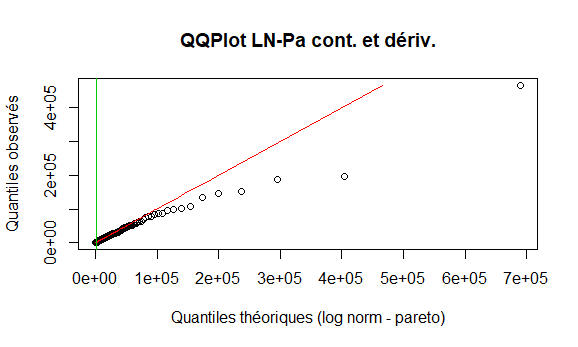
\includegraphics[scale=0.54]{Graphiques/QQ_LN_Pa_cont_dev} 
					\caption{Quantiles sur le support complet.} \label{QQplot_LN_Pa_conde}
				\end{subfigure}
				\begin{subfigure}[b]{0.40\textwidth}
					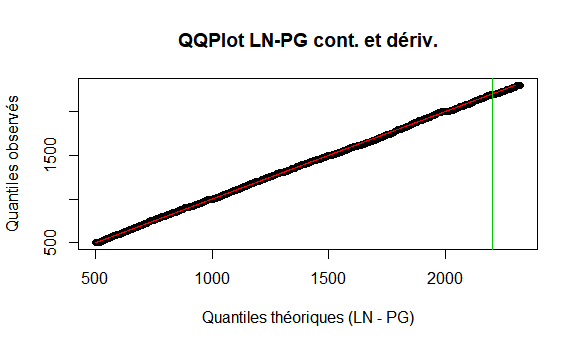
\includegraphics[scale=0.54]{Graphiques/QQ_LN_PA_contdiv_t1} 
					\caption{Quantiles de la lognormale pour $x<\theta$.} \label{QQplot_LN_Pa_conde_2}
				\end{subfigure}
				\renewcommand{\figurename}{Illustration}
				\caption{\textit{QQplots} - \texttt{norwegianfire} - LN-Pareto.}
			\end{center}
		\end{figure}
	
		Dans l'illustration \ref{QQplot_LN_Pa_conde}, on observe une bonne adéquation pour les valeurs en dessous de $100\,000$ \footnote{Rappel: Les montants affichés sont en excédent de $500\,000$ couronnes norvégiennes.}. Cependant, pour les données supérieures à ce montant, on trouve que le modèle n'est pas adéquat.  On remarque aussi que le seuil ($\theta$) estimé est relativement petit. La portion lognormale ne comprends que $61\%$ des données ($\hat{F}_n(\theta) = 0,613$, où $\hat{F}_n(\theta)$ est la fonction de répartition empirique). \\
		
		Lorsque l'on considère l'approche avec $\theta$ fixé, on observe un changement de comportement entre les valeurs de $20\,000$ et de $30\,000$ dans la fonction d'excès moyen présenté dans l'illustration \ref{Graph_Norwegianfire_MeanExcess}. On fixe $\theta = 22\,669$ (qui est le $9\,100$-ème statistique d'ordre) et on estime $\hat{\mu} =4,834\,589$, $\hat{\sigma}=1,624\,245$ et $\hat{\alpha} = 1,540\,549$.
		
		\begin{figure}[H]
			\begin{center}
				\begin{subfigure}[b]{0.45\textwidth}
					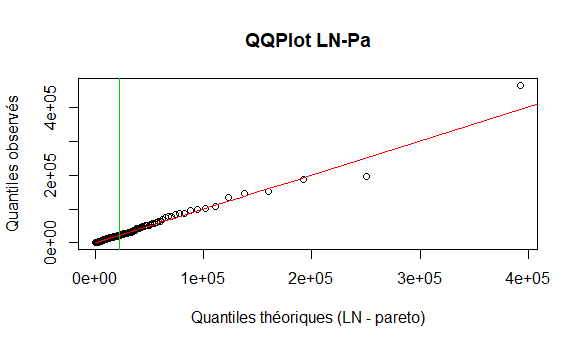
\includegraphics[scale=0.54]{Graphiques/QQ_LN_PA_choix} 
					\caption{Quantiles sur le support complet.} \label{QQplot_LN_Pa_choix}
				\end{subfigure}
				\begin{subfigure}[b]{0.4\textwidth}
					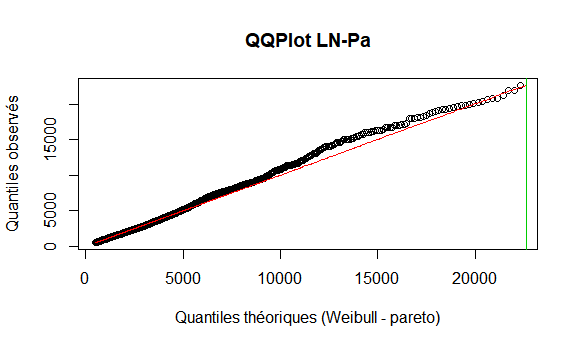
\includegraphics[scale=0.54]{Graphiques/QQ_LN_PA_choix_t1} 
					\caption{Quantiles de la lognormale pour $x<\theta$.} \label{QQplot_LN_Pa_choix_2}
				\end{subfigure}
				\renewcommand{\figurename}{Illustration}
				\caption{\textit{QQplots} - \texttt{norwegianfire} - LN-Pareto - $\theta$ fixé.}
			\end{center}
		\end{figure}
	
		De l'illustration \ref{QQplot_LN_Pa_choix_2}, on observe que l'adéquation pour la partie lognormale est un peu moins bonne que pour le modèle respectant la continuité et la dérivabilité. Cependant, pour les valeurs élevées, on surestime moins les montants de sinistres. L'ajustement est donc meilleur. Par contre, comme la densité présente un saut au point $\theta$, elle n'est pas continue et dérivable à ce point. 
		
		\paragraph{Loi composite lognormale et Pareto généralisée:} Avec la continuité et la dérivabilité au point $\theta$, on estime les paramètres et on obtient $\hat{\theta} =2\,204,333\,480$, $\hat{\lambda}=-20,958\,168$, $\hat{\alpha} =1,320\,166$ et $\hat{\sigma}= 1,143\,788$.
	
		\begin{figure}[H]
			\begin{center}
				\begin{subfigure}[b]{0.45\textwidth}
					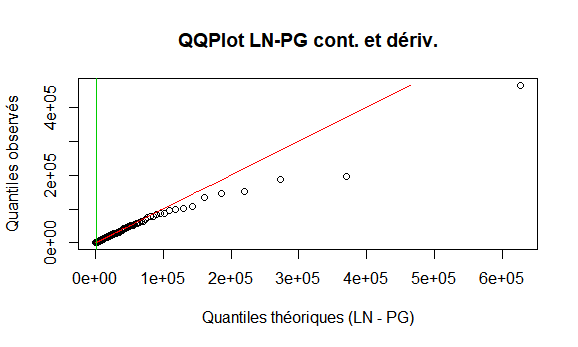
\includegraphics[scale=0.54]{Graphiques/QQ_LN_PG_condev} 
					\caption{Quantiles sur le support complet.} \label{QQplot_LN_PG_conde}
				\end{subfigure}
				\begin{subfigure}[b]{0.4\textwidth}
					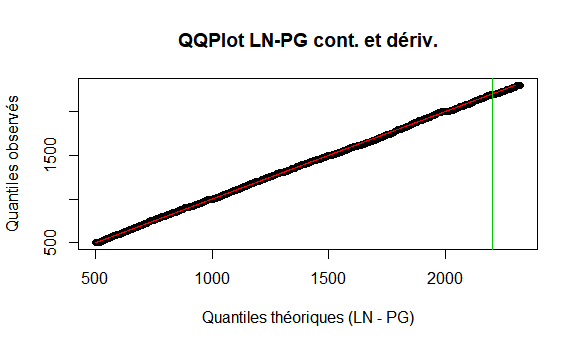
\includegraphics[scale=0.54]{Graphiques/QQ_LN_PA_contdiv_t1} 
					\caption{Quantiles de la lognormale pour $x<\theta$.} \label{QQplot_LN_PG_conde_2}
				\end{subfigure}
				\renewcommand{\figurename}{Illustration}
				\caption{\textit{QQplots} - \texttt{norwegianfire} - LN-PG.}
			\end{center}
		\end{figure}
		
		L'illustration \ref{QQplot_LN_PG_conde} montre un comportement similaire au modèle composite lognormal - Pareto simple. Toutefois, la portion lognormale comprends $81\%$ des données; ce qui est plus élevé que lorsque la deuxième loi du raccordement est une Pareto de type 1. En ignorant la continuité et la dérivabilité, on fixe $\theta = 22\,669$ et on trouve $\hat{\mu} = 4,834\,589$, $\hat{\sigma}=1,624\,245$, $\hat{\lambda} =  4\,604,525\,53$ et $\hat{\alpha} = 1,728\,66$.
		
		\begin{figure}[H]
			\begin{center}
				\begin{subfigure}[b]{0.45\textwidth}
					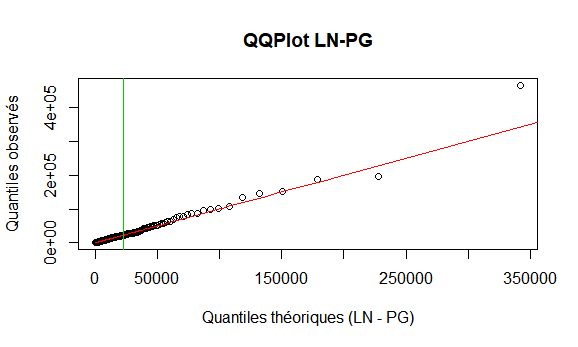
\includegraphics[scale=0.54]{Graphiques/QQ_LN_PG_choix} 
					\caption{Quantiles sur le support complet.} \label{QQplot_LN_PG_choix}
				\end{subfigure}
				\begin{subfigure}[b]{0.4\textwidth}
					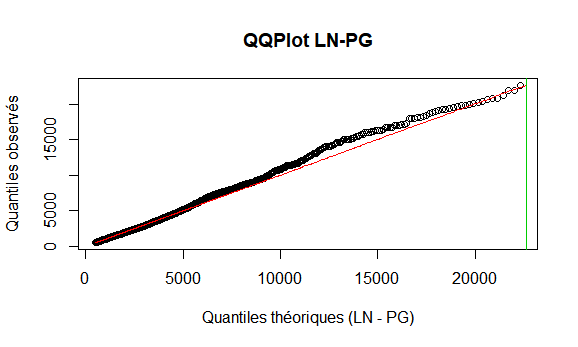
\includegraphics[scale=0.54]{Graphiques/QQ_LN_PG_choix_t1} 
					\caption{Quantiles de la lognormale pour $x<\theta$.} \label{QQplot_LN_PG_choix_2}
				\end{subfigure}
				\renewcommand{\figurename}{Illustration}
				\caption{\textit{QQplots} - \texttt{norwegianfire} - LN-PG - $\theta$ fixé.}
			\end{center}
		\end{figure}
		
		De nouveau, lorsqu'on regarde l'illustration \ref{QQplot_LN_PG_choix_2}, on voit que, lorsque l'on détermine un $\theta$ arbitrairement (sans tenir compte de la continuité et de la dérivabilité), on obtient une meilleure adéquation du modèle.
		
		\paragraph{Loi composite lognormale - Pareto - Pareto:} Les résultats obtenus avec la fonction \texttt{ConstrOptim} pour le cas où on a la continuité et la dérivabilité aux points $\theta_1$ et $\theta_2$ ne sont pas satisfaisants. Les résultats varient trop en fonction des paramètres initiaux fixés; particulièrement lorsque l'on fixe la valeur initiale de $\theta_1$ et de $\theta_2$.\\
	
		Si on applique la continuité et la dérivabilité seulement au point $\theta_1$, mais que l'on fixe $\theta_2 = 31\,728 $ on obtient $\hat{\theta_1} =1\,287,998\,125 $, $\hat{\alpha_1} =  1,282\,457$ et $\hat{\sigma}= 0,839\,466$, $\hat{\alpha_2}=1,458\,555$.
	
		\begin{figure}[H]
			\begin{center}
				\begin{subfigure}[b]{0.50\textwidth}
					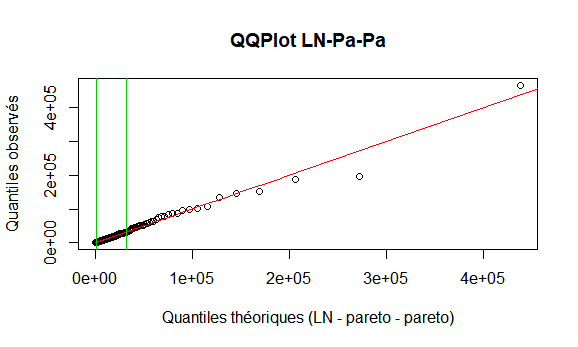
\includegraphics[scale=0.6]{Graphiques/QQ_LN_Pa_Pa_semi} 
					\caption{Quantiles sur le support complet.} \label{QQplot_LN_PaPa_semi}
				\end{subfigure}
				\begin{subfigure}[b]{0.42\textwidth}
					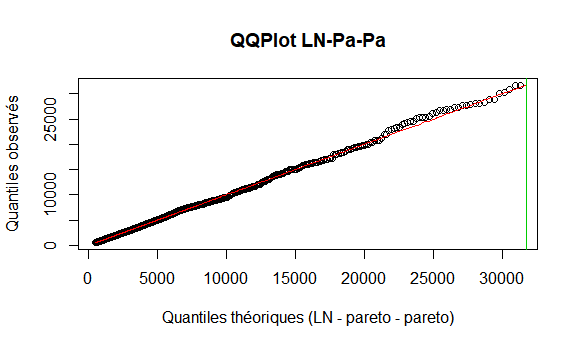
\includegraphics[scale=0.56]{Graphiques/QQ_LN_Pa_Pa_semi_t1} 
					\caption{Quantiles de la lognormale et $1^{ere}$ Pareto pour $x<\theta_2$.} \label{QQplot_LN_PaPa_semi_t1}
				\end{subfigure}
				\renewcommand{\figurename}{Illustration}
				\caption{\textit{QQplots} - \texttt{norwegianfire} - LN-Pa-Pa.}
			\end{center}
		\end{figure}
	
		Dans le illustration \ref{QQplot_LN_PaPa_semi}, on voit que les quantiles estimés sont comparables aux quantiles empiriques, même pour les valeurs très élevées.
		
		\paragraph{Loi composite Weibull et Pareto simple:} Avec la continuité et la dérivabilité au point $\theta$, on estime les paramètres et on obtient $\hat{\theta} = 1\,941,104\,864$, $\hat{\alpha} = 1,324\,505$ et $\hat{\tau}=0,595\,968$.
		
		\begin{figure}[H]
			\begin{center}
				\begin{subfigure}[b]{0.45\textwidth}
					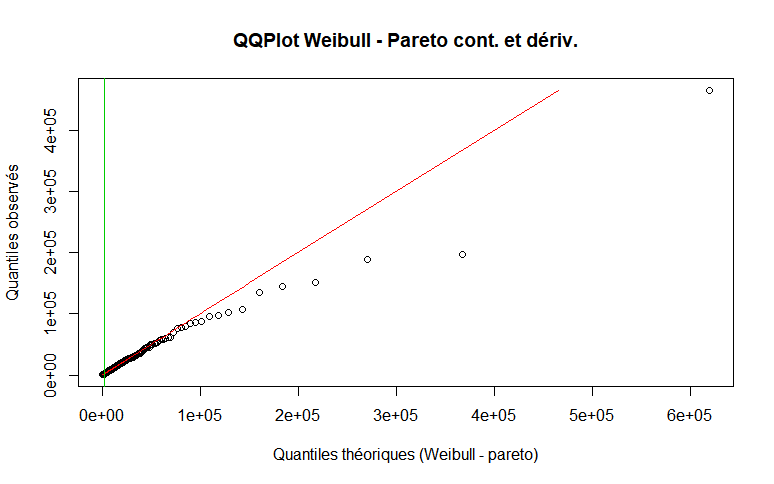
\includegraphics[scale=0.40]{Graphiques/QQ_Wei_Pa_contderiv} 
					\caption{Quantiles sur le support complet.} \label{QQplot_W_Pa_conde}
				\end{subfigure}
				\begin{subfigure}[b]{0.40\textwidth}
					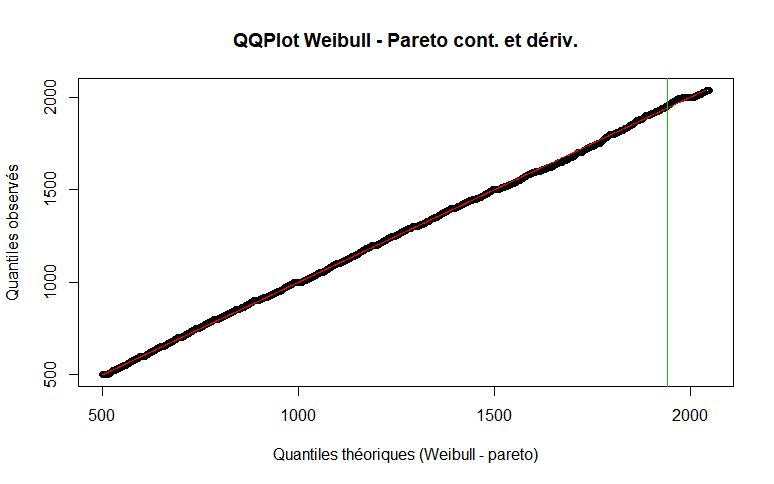
\includegraphics[scale=0.40]{Graphiques/QQ_Wei_Pa_contderiv_t1} 
					\caption{Quantiles de la Weibull pour $x<\theta$.} \label{QQplot_W_Pa_conde_2}
				\end{subfigure}
				\renewcommand{\figurename}{Illustration}
				\caption{\textit{QQplots} - \texttt{norwegianfire} - Weibull-Pareto.}
			\end{center}
		\end{figure}
		
		Le résultat est similaire à celui obtenu avec le modèle lognormal - Pareto. Cependant, le seuil $\hat{\theta}$ du modèle lognormal-Pareto est plus petit que celui du modèle Weibull-Pareto. Cela signifie que davantage de données sont attribuées à la partie Weibull. Si on fixe $\theta = 22\,669$, on obtient $\hat{\tau} =0,259\,762$, $\hat{\phi}=4,287\,200$ et $\hat{\alpha} = 1,540\,549$.
		
		\begin{figure}[H]
			\begin{center}
				\begin{subfigure}[b]{0.45\textwidth}
					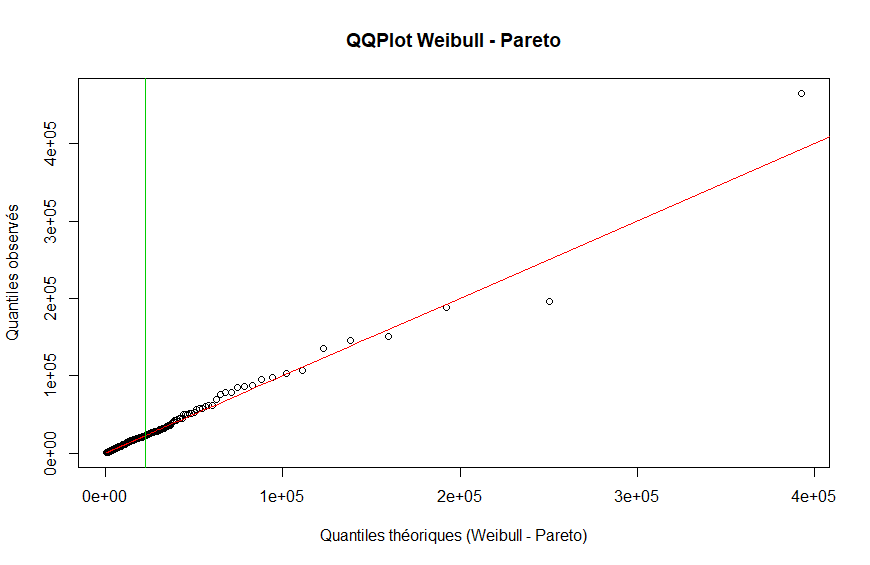
\includegraphics[scale=0.35]{Graphiques/QQ_Wei_pa_choix} 
					\caption{Quantiles sur le support complet.} \label{QQplot_Wei_pa_choix}
				\end{subfigure}
				\begin{subfigure}[b]{0.4\textwidth}
					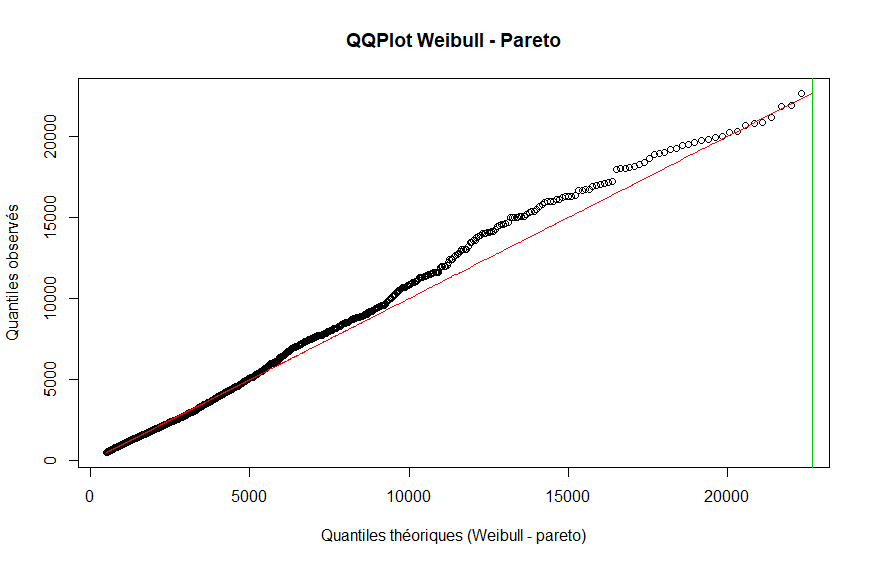
\includegraphics[scale=0.35]{Graphiques/QQ_Wei_pa_choix_t1} 
					\caption{Quantiles de la Weibull pour $x<\theta$.} \label{QQplot_Wei_pa_choix_2}
				\end{subfigure}
				\renewcommand{\figurename}{Illustration}
				\caption{\textit{QQplots} - \texttt{norwegianfire} - Weibull-Pareto - $\theta$ fixé.}\label{Wei_Pareto_Teta_fixe}
			\end{center}
		\end{figure}
	
		Dans l'illustration \ref{Wei_Pareto_Teta_fixe}, on voit que lorsque l'on fixe le seuil $\theta$, on peut obtenir une nette amélioration de l'adéquation des valeurs élevées, mais au prix d'une dégradation pour les petites valeurs.
		
		\paragraph{Loi composite Weibull et Pareto généralisée:} Avec la continuité et la dérivabilité au point $\theta$, on estime les paramètres et on obtient $\hat{\theta} = 1\,918,491\,146 $, $\hat{\alpha} = 1,327\,868 $ et $\hat{\tau}=0,599\,589 $ et $\hat{\lambda}=8,981\,391$.
		\begin{figure}[H]
			\begin{center}
				\begin{subfigure}[b]{0.45\textwidth}
					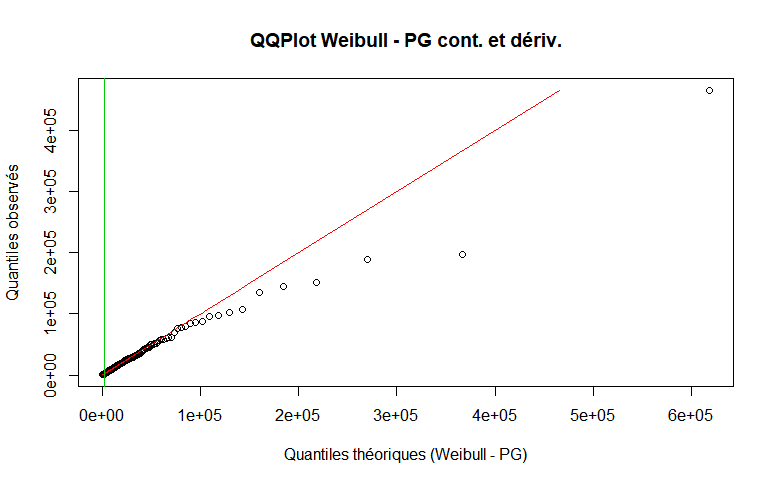
\includegraphics[scale=0.40]{Graphiques/QQ_Wei_PG_contderiv} 
					\caption{Quantiles sur le support complet.} \label{QQplot_W_PG_conde}
				\end{subfigure}
				\begin{subfigure}[b]{0.4\textwidth}
					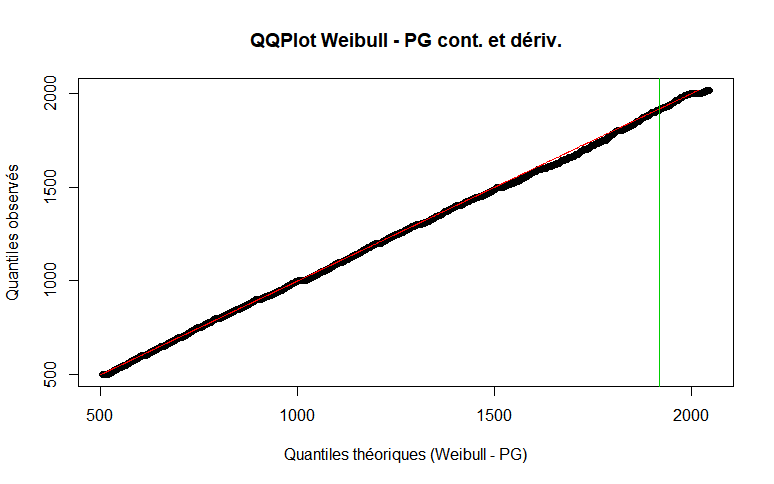
\includegraphics[scale=0.40]{Graphiques/QQ_Wei_PG_contderiv_t1} 
					\caption{Quantiles de la Weibull pour $x<\theta$.} \label{QQplot_W_PG_conde_2}
				\end{subfigure}
				\renewcommand{\figurename}{Illustration}
				\caption{\textit{QQplots} - \texttt{norwegianfire} - Weibull-PG.}
			\end{center}
		\end{figure}
		
		Les observations sont similaires à celles obtenues pour le modèle lognormal-Pareto et Weibull-Pareto.
		Si on fixe $\theta = 22\,669$, on obtient $\hat{\tau} =0,259\,762$, $\hat{\phi}=4,287\,198$, $\hat{\lambda}=4\,604,525\,53$ et $\hat{\alpha} = 1,728\,66$.
		
		\begin{figure}[H]
			\begin{center}
				\begin{subfigure}[b]{0.45\textwidth}
					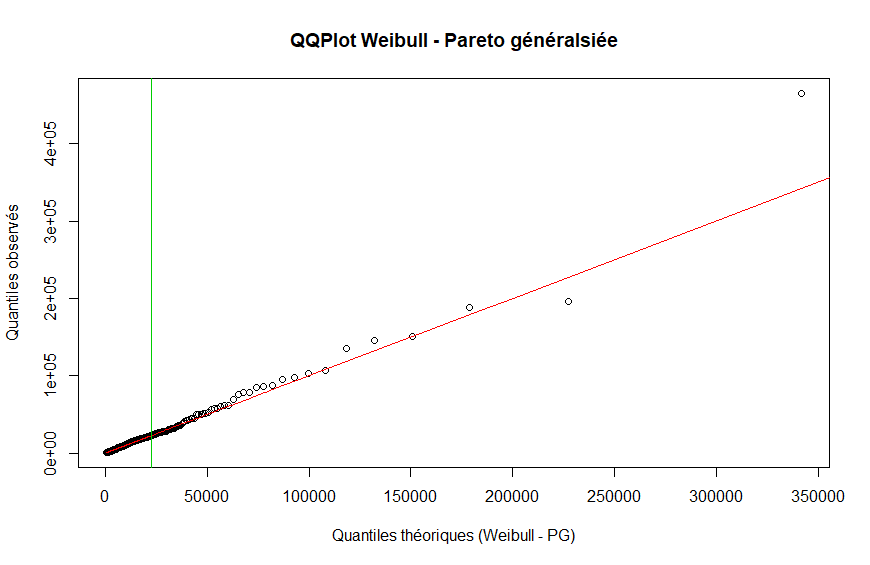
\includegraphics[scale=0.35]{Graphiques/QQ_Wei_PG_choix} 
					\caption{Quantiles sur le support complet.} \label{QQplot_Wei_PG_choix}
				\end{subfigure}
				\begin{subfigure}[b]{0.4\textwidth}
					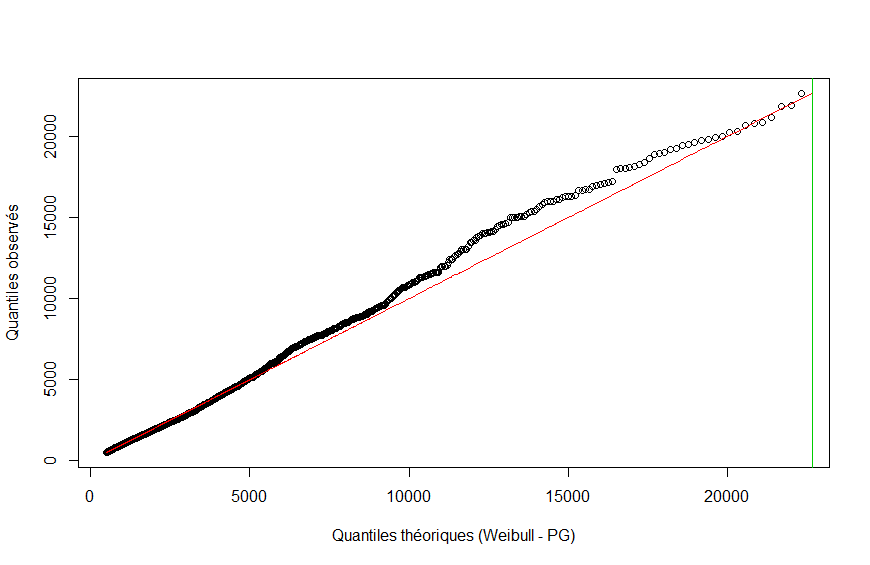
\includegraphics[scale=0.35]{Graphiques/QQ_Wei_PG_choix_t1} 
					\caption{Quantiles de la Weibull pour $x<\theta$.} \label{QQplot_Wei_PG_choix_2}
				\end{subfigure}
				\renewcommand{\figurename}{Illustration}
				\caption{\textit{QQplots} - \texttt{norwegianfire} - Weibull-Pareto - $\theta$ fixé.}\label{QQplot_Wei_PG_choix3}
			\end{center}
		\end{figure}
		À la lecture de l'illustration \ref{QQplot_Wei_PG_choix3}, on voit que les résultats sont très similaires à ceux obtenus avec les modèles utilisant une loi de Pareto simple pour représenter les grandes valeurs et dont le seuil $\theta$ est fixé.	
		
		\paragraph{Loi composite Weilbull - Pareto - Pareto:} Comme pour le modèle lognormal-Pareto-Pareto, les résultats obtenus en trouvant les deux seuils ($\theta_1$ et $\theta_2$) par optimisation numérique ne sont pas satisfaisants puisque la volatilité des paramètres obtenus est considérable. Pour cette raison, on fixe le deuxième seuil. Avec la continuité et la dérivabilité seulement au point $\theta_1$ et avec $\theta_2$ fixé à 31\,728, on obtient les paramètres $\hat{\theta_1} =1\,840,169\,474$, $\hat{\alpha_1} =  1,302\,509$ et $\hat{\tau}= 0,616\,114$, $\hat{\alpha_2}=1,458\,555$ 
		
		\begin{figure}[H]
			\begin{center}
				\begin{subfigure}[b]{0.45\textwidth}
					\includegraphics[scale=0.35]{Graphiques/QQ_Wei_Pa_Pa_semi} 
					\caption{Quantiles sur le support complet.} \label{QQplot_Wei_PaPa_semi}
				\end{subfigure}
				\begin{subfigure}[b]{0.4\textwidth}
					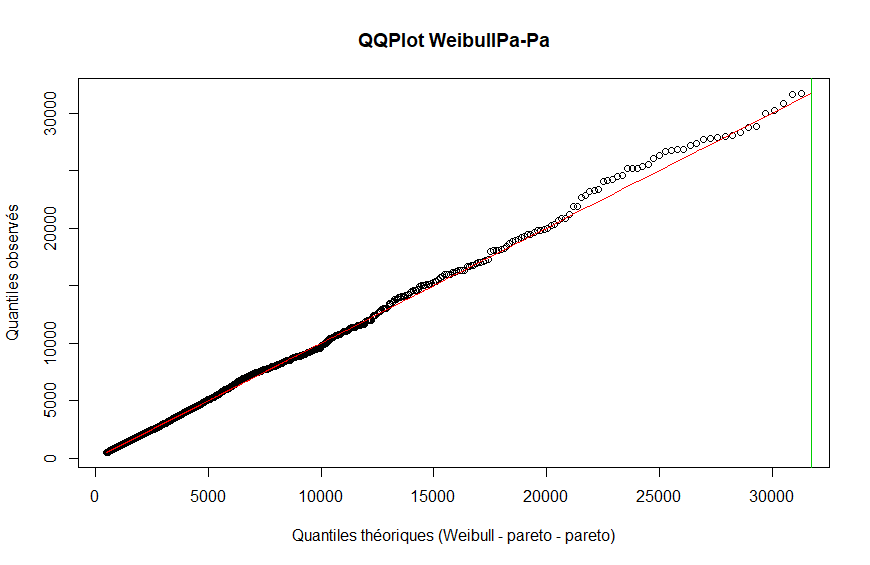
\includegraphics[scale=0.35]{Graphiques/QQ_Wei_Pa_Pa_semi_t1} 
					\caption{Quantiles de la Weibull pour $x<\theta$.} \label{QQplot_Wei_PaPa_semi_t1}
				\end{subfigure}
				\renewcommand{\figurename}{Illustration}
				\caption{\textit{QQplots} - \texttt{norwegianfire} - Weibull-Pa-Pa.}
			\end{center}
		\end{figure}
		
		\paragraph{Loi composite coxienne-2 - Pareto:} Avec la continuité au point $\theta$, on estime les paramètres et on obtient $\hat{\theta} =  6\,600,17$, $\hat{\alpha}= 1,347\,302$, $\hat{p} = 0,870\,677$, $\hat{\beta_1}=0,001\,940$ et $\hat{\beta_2}= 0,000\,427\,486$. Il faut noter que ces estimateurs ne sont pas optimaux puisqu'ils changent énormément selon les valeurs initiales choisies pour la fonction \texttt{ConstrOptim} de R. Cela peut être expliqué par le fait que la loi coxienne-2 possède trois paramètres. Si on considère que ce phénomène est similaire à celui obtenu avec les raccordements de trois lois, on peut conclure que la fonction d'optimisation numérique utilisée perd beaucoup de précision lorsqu'il y a plus de quatre paramètres à estimer.
		\begin{figure}[H]
			\begin{center}
				\begin{subfigure}[b]{0.45\textwidth}
					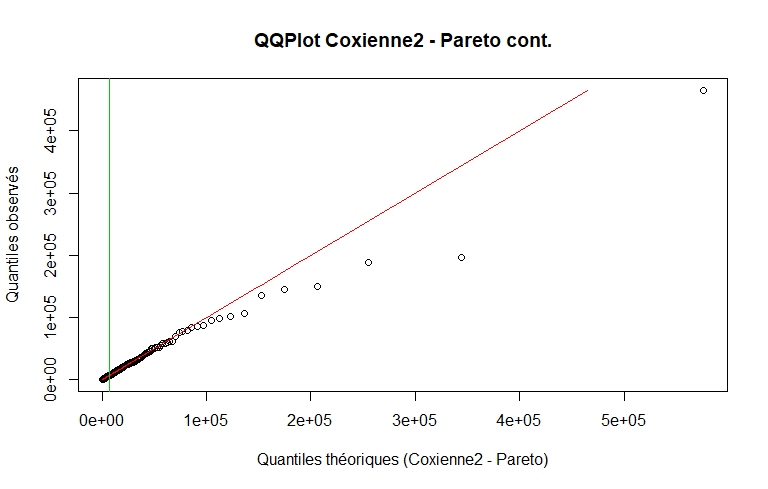
\includegraphics[scale=0.40]{Graphiques/QQ_Cox_Pa_cont} 
					\caption{Quantiles sur le support complet.} \label{QQplot_Cox_Pa_con}
				\end{subfigure}
				\begin{subfigure}[b]{0.4\textwidth}
					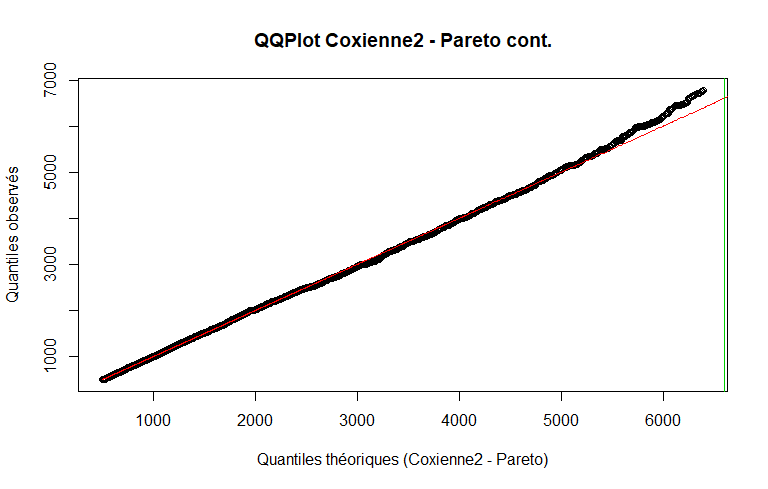
\includegraphics[scale=0.40]{Graphiques/QQ_Cox_Pa_cont_t1} 
					\caption{Quantiles de la cox-2 pour $x<\theta$.} \label{QQplot_Cox_Pa_con_2}
				\end{subfigure}
				\renewcommand{\figurename}{Illustration}
				\caption{\textit{QQplots} - \texttt{norwegianfire} - Coxienne-2 - Pareto.}\label{QQplot_Cox_Pa_con_3}
			\end{center}
		\end{figure}
		
		Même si les valeurs ne sont pas nécessairement optimales, on voit malgré tout dans l'illustration \ref{QQplot_Cox_Pa_con_3} que les valeurs inférieures à 100\,000 sont bien modélisés, mais que, pour les valeurs plus élevées, on obtient une surestimation des observations. \\
		
		Si on ignore la continuité, on fixe $\theta = 22\,669$ et on estime $\hat{\alpha} = 1,540\,549$, $\hat{p} =0,904\,056\,917$, $\hat{\beta_1}=0,001\,696\,942$ et $\hat{\beta_2} = 0,000\,262\,067$.
		
		\begin{figure}[H]
			\begin{center}
				\begin{subfigure}[b]{0.45\textwidth}
					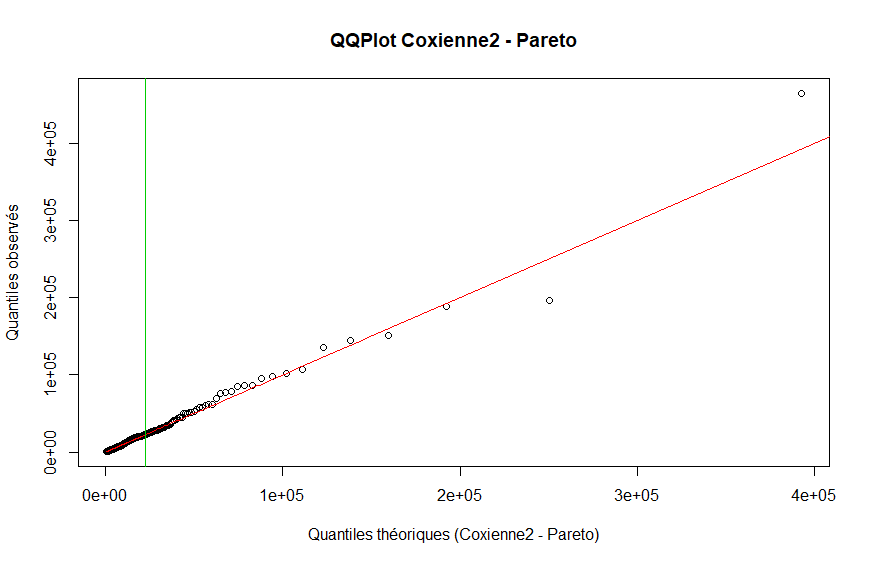
\includegraphics[scale=0.35]{Graphiques/QQ_Cox_pa_choix} 
					\caption{Quantiles sur le support complet.} \label{QQplot_Cox_pa_choix}
				\end{subfigure}
				\begin{subfigure}[b]{0.4\textwidth}
					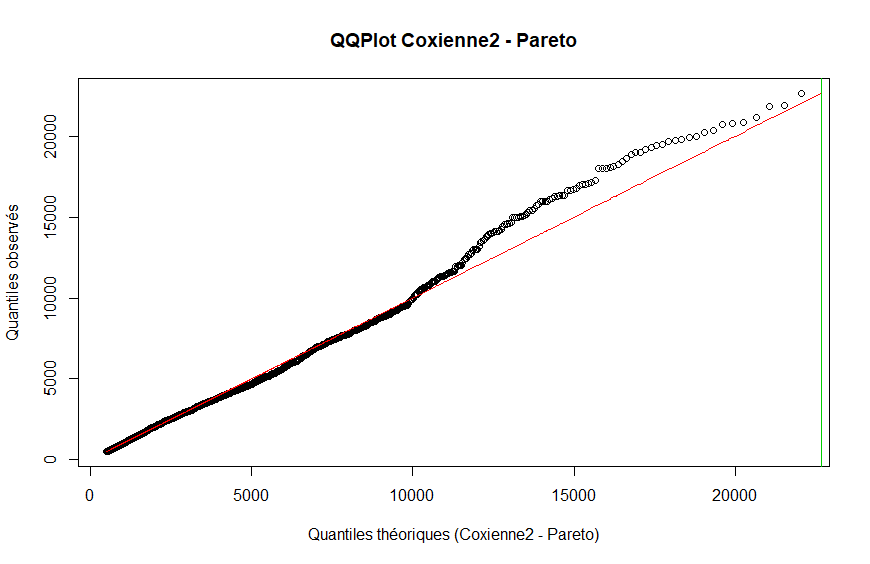
\includegraphics[scale=0.35]{Graphiques/QQ_Cox_pa_choix_t1} 
					\caption{Quantiles de la cox-2 pour $x<\theta$.} \label{QQplot_Cox_pa_choix_2}
				\end{subfigure}
				\renewcommand{\figurename}{Illustration}
				\caption{\textit{QQplots} - \texttt{norwegianfire} - Coxienne-2 - Pareto - $\theta$ fixé.}
			\end{center}
		\end{figure}
		L'ajustement est considérablement moins bon pour la partie coxienne-2, mais meilleur pour les valeurs très élevées.
		 
		\paragraph{Loi composite coxienne-2 - Pareto généralisée:} Avec la continuité au point $\theta$ on estime les paramètres et on obtient $\hat{\theta} =  7\,258,73$, $\hat{\lambda}=1\,057,91$, $\hat{\alpha}= 1,494\,710$ $\hat{p} = 0,561\,217$, $\hat{\beta_1}=0,001\,907\,145$ et $\hat{\beta_2}= 0,000\,408\,597$.
		
		\begin{figure}[H]
			\begin{center}
				\begin{subfigure}[b]{0.45\textwidth}
					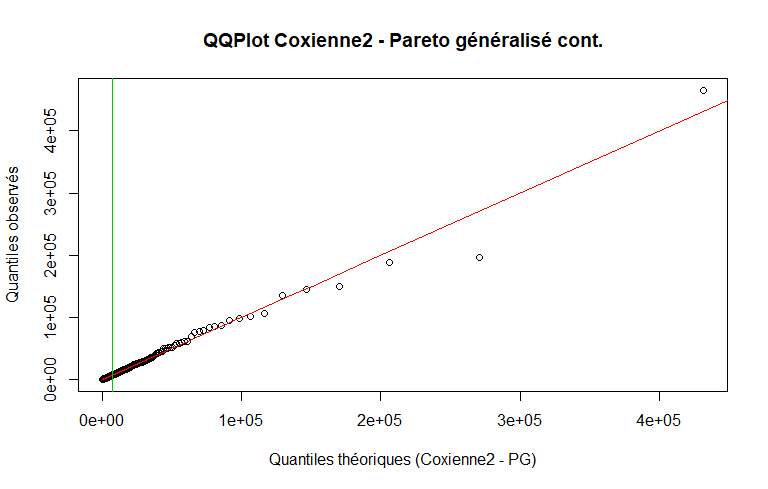
\includegraphics[scale=0.40]{Graphiques/QQ_Cox_PG_cont} 
					\caption{Quantiles sur le support complet.} \label{QQplot_Cox_PG_con}
				\end{subfigure}
				\begin{subfigure}[b]{0.4\textwidth}
					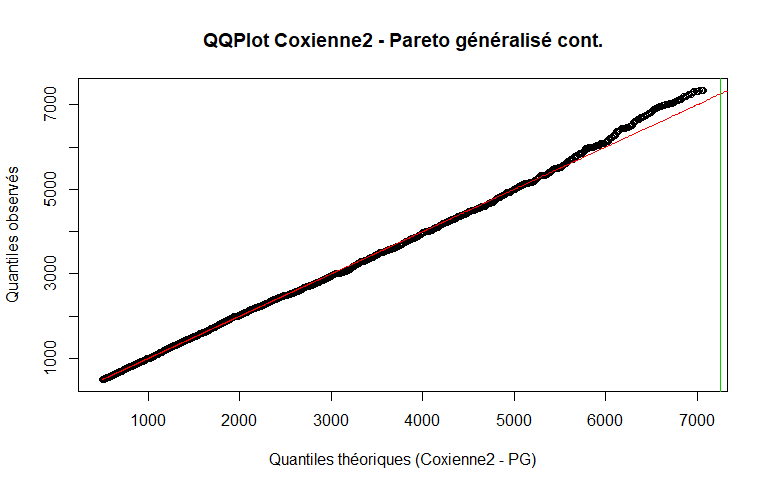
\includegraphics[scale=0.40]{Graphiques/QQ_Cox_PG_cont_t1} 
					\caption{Quantiles de la cox-2 pour $x<\theta$.} \label{QQplot_Cox_PG_con_2}
				\end{subfigure}
				\renewcommand{\figurename}{Illustration}
				\caption{\textit{QQplots} - \texttt{norwegianfire} - Coxienne-2 - PG. }
			\end{center}
		\end{figure}
		
		L'ajustement est acceptable pour les deux parties du raccordement. Si on ignore la continuité, on fixe $\theta = 22\,669$ et on estime $\hat{\lambda}=4\,604,525\,53$, $\hat{\alpha} = 1,728\,66$, $\hat{p} =0,904\,056\,917$, $\hat{\beta_1}=0,001\,696\,942$ et $\hat{\beta_2} = 0,000\,262\,067$.
		
		\begin{figure}[H]
			\begin{center}
				\begin{subfigure}[b]{0.45\textwidth}
					\includegraphics[scale=0.40]{Graphiques/QQ_Cox_PG_choix} 
					\caption{Quantiles sur le support complet.} \label{QQplot_Cox_PG_choix}
				\end{subfigure}
				\begin{subfigure}[b]{0.4\textwidth}
					\includegraphics[scale=0.40]{Graphiques/QQ_Cox_PG_choix_t1} 
					\caption{Quantiles de la cox-2 pour $x<\theta$.} \label{QQplot_Cox_PG_choix_2}
				\end{subfigure}
				\renewcommand{\figurename}{Illustration}
				\caption{\textit{QQplots} - \texttt{norwegianfire} - Coxienne-2 - PG - $\theta$ fixé.}
			\end{center}
		\end{figure}
		L'ajustement est considérablement moins bon pour la partie coxienne-2, mais meilleur pour les valeurs élevées.
		 
	\subsubsection{\texttt{secura}}	
		
		\paragraph{Loi composite lognormale - Pareto:} Avec la continuité et la dérivabilité au point $\theta$ on estime les paramètres et on obtient $\hat{\theta} = 3,263\,838$, $\hat{\alpha} = 3,540\,522$, $\hat{\mu}=0,569\,56$  et $\hat{\sigma}=0,416\,216$.
		
		\begin{figure}[H]
			\begin{center}
				\begin{subfigure}[b]{0.45\textwidth}
					\includegraphics[scale=0.65]{Graphiques/QQ_LN_Pa_cont_dev_secura} 
					\caption{Quantiles sur le support complet.} \label{QQplot_LN_Pa_conde_sec}
				\end{subfigure}
				\begin{subfigure}[b]{0.4\textwidth}
					\includegraphics[scale=0.65]{Graphiques/QQ_LN_PA_contdiv_t1_secura} 
					\caption{Quantiles de la lognormale pour $x<\theta$.} \label{QQplot_LN_Pa_conde_2_sec}
				\end{subfigure}
				\renewcommand{\figurename}{Illustration}
				\caption{\textit{QQplots} - \texttt{secura} - Lognormale-Pareto.}
			\end{center}
		\end{figure}
		L'illustration \ref{QQplot_LN_Pa_conde_sec} montre un bon ajustement, même pour les valeurs élevées. Seulement les deux dernières statistiques d'ordre sont fortement surestimées. La portion lognormale comprend 62\% des données. \\
		
		Si on fixe le seuil, on regarde la fonction d'excès moyen présentée dans l'illustration \ref{Graph_Secura_MeanExcess} et on observe un changement de comportement à partir du point $3$. Conséquemment, on fixe $\theta = 3,001\,082$ et on estime $\hat{\mu} =0,574\,117$, $\hat{\sigma}=0,510\,611$ et $\hat{\alpha} = 3,279\,089$.
		
		\begin{figure}[H]
			\begin{center}
				\begin{subfigure}[b]{0.45\textwidth}
					\includegraphics[scale=0.65]{Graphiques/QQ_LN_PA_choix_secura} 
					\caption{Quantiles sur le support complet.} \label{QQplot_LN_Pa_choix_secrua}
				\end{subfigure}
				\begin{subfigure}[b]{0.4\textwidth}
					\includegraphics[scale=0.65]{Graphiques/QQ_LN_PA_choix_t1_secura} 
					\caption{Quantiles de la lognormale pour $x<\theta$.} \label{QQplot_LN_Pa_choix_2_secrua}
				\end{subfigure}
				\renewcommand{\figurename}{Illustration}
				\caption{\textit{QQplots} - \texttt{secura} - Lognormale-Pareto - $\theta$ fixé.}
			\end{center}
		\end{figure}
		
		L'ajustement est très similaire à celui présenté dans l'illustration \ref{QQplot_LN_Pa_conde_sec}, car on a fixe un $\theta$ proche de $\hat{\theta}$. Il est donc plus intéressant de choisir le modèle respectant les restrictions de continuité et de dérivabilité.  	

		\paragraph{Loi composite lognormale - Pareto généralisée:} Avec la continuité et la dérivabilité au point $\theta$ on estime les paramètres et on obtient $\hat{\theta} =3,150\,354$, $\hat{\lambda}=1,332\,734$ $\hat{\alpha} =4,896\,833 $ et $\hat{\sigma}= 0,418\,792$.
		\begin{figure}[H]
			\begin{center}
				\begin{subfigure}[b]{0.45\textwidth}
					\includegraphics[scale=0.65]{Graphiques/QQ_LN_PG_condev_Secura} 
					\caption{Quantiles sur le support complet.} \label{QQplot_LN_PG_conde_Sec}
				\end{subfigure}
				\begin{subfigure}[b]{0.4\textwidth}
					\includegraphics[scale=0.65]{Graphiques/QQ_LN_PA_contdiv_t1_Secura} 
					\caption{Quantiles de la lognormale pour $x<\theta$.} \label{QQplot_LN_PG_conde_2_Sec}
				\end{subfigure}
				\renewcommand{\figurename}{Illustration}
				\caption{\textit{QQplots} - \texttt{secura} - Lognormale-PG.}\label{QQplot_LN_PG_conde_Sec3}
			\end{center}
		\end{figure}
		
		Dans l'illustration \ref{QQplot_LN_PG_conde_Sec} on observe que le modèle avec une Pareto généralisée sous-estime davantage les grandes valeurs que le modèle avec une loi de Pareto simple. En revanche, la dernière valeur est beaucoup mieux prédite. La partie de la lognormale comprends 88\% des données, ce qui est plus élevé que lorsque l'on utilise la loi de Pareto simple pour modéliser les grandes valeurs. \\
		
		Si on ignore la continuité et la dérivabilité, on fixe $\theta = 3$ et on estime $\hat{\mu} =0,574\,117$, $\hat{\sigma}=0,510\,611$, $\hat{\lambda} =  23,788\,65$ et $\hat{\alpha} = 22,889\,47$. Il faut noter que $\hat{\alpha}$ est très grand pour une Pareto généralisée. Pour cette raison, la portion Pareto ressemble beaucoup à une loi gamma.
		
		\begin{figure}[H]
			\begin{center}
				\begin{subfigure}[b]{0.45\textwidth}
					\includegraphics[scale=0.65]{Graphiques/QQ_LN_PG_choix_secura} 
					\caption{Quantiles sur le support complet.} \label{QQplot_LN_PG_choix_secura}
				\end{subfigure}
				\begin{subfigure}[b]{0.4\textwidth}
					\includegraphics[scale=0.65]{Graphiques/QQ_LN_PG_choix_t1_secura} 
					\caption{Quantiles de la lognormale pour $x<\theta$.} \label{QQplot_LN_PG_choix_2_secura}
				\end{subfigure}
				\renewcommand{\figurename}{Illustration}
				\caption{\textit{QQplots} - \texttt{secura} - Lognormale-PG - $\theta$ fixé.}
			\end{center}
		\end{figure}
		Dans l'illustration \ref{QQplot_LN_PG_choix_secura}, on voit que l'adéquation globale lorsque l'on fixe le point $\theta$ est très similaire à celle lorsqu'on assume la continuité et la dérivabilité. Cependant, pour la plus grande valeur, celle-ci est mieux représentée lorsque le seuil est fixé.
		
		\paragraph{Loi composite lognormale - Pareto - Pareto:} Avec la continuité et la dérivabilité appliquée seulement au point $\theta_1$ et avec le point $\theta_2$ fixé à $4,050\,863$, on obtient $\hat{\theta_1} =2,247\,724 $, $\hat{\alpha_1} = 2,788\,940$, $\hat{\sigma}= 0,319\,746$ et $\hat{\alpha_2}=3,639\,318$.
		
		\begin{figure}[H]
			\begin{center}
				\begin{subfigure}[b]{0.45\textwidth}
					\includegraphics[scale=0.65]{Graphiques/QQ_LN_Pa_Pa_semi_Secura} 
					\caption{Quantiles sur le support complet.} \label{QQplot_LN_PaPa_semi_Sec}
				\end{subfigure}
				\begin{subfigure}[b]{0.4\textwidth}
					\includegraphics[scale=0.65]{Graphiques/QQ_LN_Pa_Pa_semi_t1_Secura} 
					\caption{Quantiles de la lognormale et $1^{ere}$ Pareto pour $x<\theta_2$.} \label{QQplot_LN_PaPa_semi_t1_sec}
				\end{subfigure}
				\renewcommand{\figurename}{Illustration}
				\caption{\textit{QQplots} - \texttt{secura} - Lognormale-Pa-Pa.}
			\end{center}
		\end{figure}
		Si on compare les illustrations \ref{QQplot_LN_PaPa_semi_Sec} et \ref{QQplot_LN_PG_conde_Sec}, on voit qu'il ne semble pas y avoir de réel avantage à utiliser un raccordement de trois lois pour modéliser les données. En effet, à première vue, il ne semble pas y avoir de différence significative pour les points se situant entre les deux seuils, de même que pour les valeurs élevées. 
		
		\paragraph{Loi composite Weibull - Pareto simple:} Avec la continuité et la dérivabilité au point $\theta$, on estime les paramètres et on obtient $\hat{\theta} = 2,992\,916$, $\hat{\alpha} = 3,571\,568$ et $\hat{\tau}= 2,034\,399$.
		\begin{figure}[H]
			\begin{center}
				\begin{subfigure}[b]{0.45\textwidth}
					\includegraphics[scale=0.55]{Graphiques/QQ_Wei_Pa_contderiv_secura} 
					\caption{Quantiles sur le support complet.} \label{QQplot_W_Pa_conde_secura}
				\end{subfigure}
				\begin{subfigure}[b]{0.4\textwidth}
					\includegraphics[scale=0.55]{Graphiques/QQ_Wei_Pa_contderiv_t1_secura} 
					\caption{Quantiles de la Weibull pour $x < \theta$.} \label{QQplot_W_Pa_conde_2_secura}
				\end{subfigure}
				\renewcommand{\figurename}{Illustration}
				\caption{\textit{QQplots} - \texttt{secura} - Weibull-Pareto.}
			\end{center}
		\end{figure}
		
		Visuellement, il est difficile d'identifier une différence entre ce modèle et le modèle lognormale. Par contre, le seuil $\theta$ est plus petit pour le modèle avec une loi lognormale que pour celui avec une loi Weibull. \\
		
		Si on fixe $\theta = 3$ et on estime $\hat{\tau} =1,718\,838$, $\hat{\phi}=1,811\,440$ et $\hat{\alpha} = 3,279\,089$.
		
		\begin{figure}[H]
			\begin{center}
				\begin{subfigure}[b]{0.45\textwidth}
					\includegraphics[scale=0.55]{Graphiques/QQ_Wei_pa_choix_secura} 
					\caption{Quantiles sur le support complet.} \label{QQplot_Wei_pa_choix_secura}
				\end{subfigure}
				\begin{subfigure}[b]{0.4\textwidth}
					\includegraphics[scale=0.55]{Graphiques/QQ_Wei_pa_choix_t1_secura} 
					\caption{Quantiles de la Weibull pour $x < \theta$.} \label{QQplot_Wei_pa_choix_2_secura}
				\end{subfigure}
				\renewcommand{\figurename}{Illustration}
				\caption{\textit{QQplots} - \texttt{secura} - Weibull-Pareto - $\theta$ fixé.}
			\end{center}
		\end{figure}
	
		\paragraph{Loi composite Weibull - Pareto généralisée:} Avec la continuité et la dérivabilité au point $\theta$ on estime les paramètres et on obtient $\hat{\theta} = 2,944\,522 $, $\hat{\alpha} =  3,963\,976 $ et $\hat{\tau}=2,034\,156 $ et $\hat{\lambda}=0,372\,262$.
	
		\begin{figure}[H]
			\begin{center}
				\begin{subfigure}[b]{0.45\textwidth}
					\includegraphics[scale=0.55]{Graphiques/QQ_Wei_PG_contderiv_secura} 
					\caption{Quantiles sur le support complet.} \label{QQplot_W_PG_conde_secura}
				\end{subfigure}
				\begin{subfigure}[b]{0.4\textwidth}
					\includegraphics[scale=0.55]{Graphiques/QQ_Wei_PG_contderiv_t1_secura} 
					\caption{Quantiles de la Weibull pour $x < \theta$.} \label{QQplot_W_PG_conde_2_secura}
				\end{subfigure}
				\renewcommand{\figurename}{Illustration}
				\caption{\textit{QQplots} - \texttt{secura} - Weibull-PG.}
			\end{center}
		\end{figure}
		
		Si on fixe $\theta =3$, on obtient $\hat{\tau} =1,718\,838$, $\hat{\phi}=1,811\,440$, $\hat{\lambda}=23,788\,65$ et $\hat{\alpha} = 22,889\,47$.
		
		\begin{figure}[H]
			\begin{center}
				\begin{subfigure}[b]{0.45\textwidth}
					\includegraphics[scale=0.55]{Graphiques/QQ_Wei_PG_choix_secura} 
					\caption{Quantiles sur le support complet.} \label{QQplot_Wei_PG_choix_secura}
				\end{subfigure}
				\begin{subfigure}[b]{0.4\textwidth}
					\includegraphics[scale=0.55]{Graphiques/QQ_Wei_PG_choix_t1_secura} 
					\caption{Quantiles de la Weibull pour $x < \theta$.} \label{QQplot_Wei_PG_choix_2_secura}
				\end{subfigure}
				\renewcommand{\figurename}{Illustration}
				\caption{\textit{QQplots} - \texttt{secura} - Weibull-PG - $\theta$ fixé.}
			\end{center}
		\end{figure}
		Mêmes observations que dans les section précédentes.
		
		\paragraph{Loi composite Weilbull - Pareto - Pareto:} Comme il a été conclu à la page \pageref{QQplot_Cox_Pa_con_3} les lois composites avec plus de quatre paramètres ont une forte volatilité. Malgré tout, si on assume la continuité et la dérivabilité seulement au point $\theta_1$ et qu'on fixe $\theta_2 = 4 $, on obtient $\hat{\theta_1} =3,060\,834$, $\hat{\alpha_1} =  3,886\,627$ et $\hat{\tau}= 2,054\,345$, $\hat{\alpha_2}=3,639\,318$. 
		
		\begin{figure}[H]
			\begin{center}
				\begin{subfigure}[b]{0.45\textwidth}
					\includegraphics[scale=0.55]{Graphiques/QQ_Wei_Pa_Pa_semi_secura} 
					\caption{Quantiles sur le support complet.} \label{QQplot_Wei_PaPa_semi_secura}
				\end{subfigure}
				\begin{subfigure}[b]{0.4\textwidth}
					\includegraphics[scale=0.55]{Graphiques/QQ_Wei_Pa_Pa_semi_t1_secura} 
					\caption{Quantiles de la Weibull et $1^{ere}$ Pareto pour $x<\theta_2$.} \label{QQplot_Wei_PaPa_semi_t1_secura}
				\end{subfigure}
				\renewcommand{\figurename}{Illustration}
				\caption{\textit{QQplots} - \texttt{secura} - Weibull-Pa-Pa.}
			\end{center}
		\end{figure}
	
		\paragraph{Loi composite coxienne-2 - Pareto:} Avec la continuité au point $\theta$ on estime les paramètres et on obtient $\hat{\theta} = 2,274\,088$, $\hat{\alpha}= 3,236\,183$, $\hat{p} = 0,936\,706$, $\hat{\beta_1}=0,386\,105$ et $\hat{\beta_2}= 0,000\,012\,679$. Rappelons que ces valeurs ne sont pas optimales puisqu'elles varient beaucoup en fonction des valeurs initiales choisies pour la fonction \texttt{ConstrOptim} de R. 
		\begin{figure}[H]
			\begin{center}
				\begin{subfigure}[b]{0.45\textwidth}
					\includegraphics[scale=0.40]{Graphiques/QQ_Cox_Pa_cont_secura} 
					\caption{Quantiles sur le support complet.} \label{QQplot_Cox_Pa_con_sec}
				\end{subfigure}
				\begin{subfigure}[b]{0.4\textwidth}
					\includegraphics[scale=0.40]{Graphiques/QQ_Cox_Pa_cont_t1_secura} 
					\caption{Quantiles de la coxi-2 pour$ x<\theta$.} \label{QQplot_Cox_Pa_con_2_sec}
				\end{subfigure}
				\renewcommand{\figurename}{Illustration}
				\caption{\textit{QQplots} - \texttt{secura} - Coxienne-2 - Pareto.}
			\end{center}
		\end{figure}
		
		Même si les valeurs ne sont pas nécessairement optimales, l'illustration \ref{QQplot_Cox_Pa_con} nous montre un bon ajustement, sauf aux valeurs élevées.  \\
		
		Si on ignore la continuité, on fixe $\theta = 22\,669$ et on estime $\hat{\alpha} = 1,540\,549$, $\hat{p} =0,757\,712$, $\hat{\beta_1}=0,934\,538$ et $\hat{\beta_2} =0,000\,000\,013$.	
		\begin{figure}[H]
			\begin{center}
				\begin{subfigure}[b]{0.45\textwidth}
					\includegraphics[scale=0.40]{Graphiques/QQ_Cox_pa_choix_secura} 
					\caption{Quantiles sur le support complet.} \label{QQplot_Cox_pa_choix_sec}
				\end{subfigure}
				\begin{subfigure}[b]{0.4\textwidth}
					\includegraphics[scale=0.40]{Graphiques/QQ_Cox_pa_choix_t1_secura} 
					\caption{Quantiles de la cox-2 pour $x<\theta$.} \label{QQplot_Cox_pa_choix_2_sec}
				\end{subfigure}
				\renewcommand{\figurename}{Illustration}
				\caption{\textit{QQplots} - \texttt{secura} - Coxienne-2 - Pareto - $\theta$ fixé.}
			\end{center}
		\end{figure}
		L'ajustement est considérablement moins bon pour la partie coxienne-2, mais meilleur pour les valeurs élevées.\\
	
		\paragraph{Loi composite coxienne-2 - Pareto généralisée:} Avec la continuité au point $\theta$ on estime les paramètres et on obtient $\hat{\theta} =  2,669\,877$, $\hat{\lambda}=0,000\,005\,118$, $\hat{\alpha}= 3,695\,810$, $\hat{p} = 0,756\,522$, $\hat{\beta_1}=0,658\,269$ et $\hat{\beta_2}= 0,000\,000\,379\,863$. Encore ici, comme il y a six paramètres à estimer, il faut considérer la forte volatilité de ceux-ci.
		\begin{figure}[H]
			\begin{center}
				\begin{subfigure}[b]{0.45\textwidth}
					\includegraphics[scale=0.40]{Graphiques/QQ_Cox_PG_cont_secura} 
					\caption{Quantiles sur le support complet.} \label{QQplot_Cox_PG_con_sec}
				\end{subfigure}
				\begin{subfigure}[b]{0.4\textwidth}
					\includegraphics[scale=0.40]{Graphiques/QQ_Cox_PG_cont_t1_secura} 
					\caption{Quantiles de la cox-2 pour $x<\theta$.} \label{QQplot_Cox_PG_con_2_sec}
				\end{subfigure}
				\renewcommand{\figurename}{Illustration}
				\caption{\textit{QQplots} - \texttt{secura} - Coxienne-2 - PG.}
			\end{center}
		\end{figure}
	
	\subsubsection{\texttt{danish}}
		\paragraph{Loi de Pareto simple:}
		Comme il est mentionné dans la section \ref{Section_AnalysePreliminaire} et comme le confirme l'illustration \ref{QQplot_Par_t_Danish}, une simple loi de Pareto de type 1 fait un travail remarquable pour modéliser l'ensemble de la distribution de la base de données \texttt{danish}. Les paramètres de ce modèle sont $\hat{\lambda} =0,923\,065$ et $\hat{\alpha} =1,270\,676$.
		\begin{figure}[H]
			\centering
			\includegraphics[scale=0.70]{Graphiques/QQ_Pa_Danish}  
			\renewcommand{\figurename}{Illustration}
			\caption{\textit{QQplots} - \texttt{danish} - Pareto.} \label{QQplot_Par_t_Danish}
		\end{figure}

		Compte tenu qu'un modèle très simple réussit à donner d'aussi bons résultats, il est superflu de tester des modèles plus complexes qui ne risquent pas d'apporter d'amélioration significative.
			
	\subsection{Choix de modèle avec test d'adéquation}\label{Sect_Test_Adequation}
		Comme l'analyse graphique ne donne qu'un aperçu de l'adéquation des modèles, il est nécessaire de procéder à des tests statistiques pour compléter l'analyse des résultats et pour choisir un modèle propre à chacune des bases de données. À cet effet, on se base sur les trois tests suivants:
		\begin{enumerate}
			\item Anderson-Darling test
			\item AIC
			\item BSC
		\end{enumerate}  
		Comme le test Anderson-Darling est plus adéquat que le test Kolmogorov-Smirnov pour les distributions à queue lourde, il n'est pas nécessaire d'utiliser ce dernier. 
		
		\subsubsection{\texttt{norwegianfire}} 
		\begin{sloppypar}Le tableau \ref{TAB_TestGOF_NF} regroupe les résultats des trois tests pour chaque modèle de la base de données \texttt{norwegianfire}. Les modèles "$\theta$ fixé" désignent les modèles où on a choisit et fixé le point $\theta$ en ignorant la continuité et la dérivabilité. 
		\end{sloppypar}
		\begin{table}[H]
			\begin{center}
				\begin{tabular}{|l|cccc|}
					\hline
					Modèle sévérité          &         AIC         &         BSC         & A-D statistique & A-D valeur-p \\ \hline
					LN-Pa                    &     147\,702,2      &     147\,723,5      &       Inf       & 6,535236e-08 \\
					LN-Pa $\theta$ fixé      &     147\,733,7      &     147\,755,1      &       Inf       & 6,535236e-08 \\
					LN-PG                    &     147\,704,2      &     147\,732,7      &       Inf       & 6,535236e-08 \\
					LN-PG $\theta$ fixé      &     147\,733,6      &     147\,755,0      &       Inf       & 6,535236e-08 \\
					LN-Pa-Pa                 &     147\,706,4      &     147\,734,9      &       Inf       & 6,535236e-08 \\
					\textbf{Weibull-Pa }     & \textbf{147\,699,8} & \textbf{147\,721,2} & \textbf{89,225} & 6,535236e-08 \\
					Weibull-Pa $\theta$ fixé &     147\,746,2      &     147\,767,6      &       Inf       & 6,535236e-08 \\
					Weibull-PG               &     147\,701,8      &     147\,730,3      &       Inf       & 6,535236e-08 \\
					Weibull-Pa $\theta$ fixé &     147\,748,1      &     147\,776,6      &       Inf       & 6,535236e-08 \\
					Weibull-Pa-Pa            &     147\,700,4      &     147\,728,9      &       Inf       & 6,535236e-08 \\
					Cox2-Pa                  &     147\,721,7      &     147\,757,4      &   19\,781,082   & 6,535236e-08 \\
					Cox2-Pa $\theta$ fixé    &     147\,757,3      &     147\,785,8      &       Inf       & 6,535236e-08 \\
					Cox2-PG                  &     147\,725,8      &     147\,768,5      &   20\,747,655   & 6,535236e-08 \\
					Cox2-PG $\theta$ fixé    &     147\,759,1      &     147\,794,7      &       Inf       & 6,535236e-08 \\ \hline
				\end{tabular}
			\renewcommand{\tablename}{Tableau}
			\caption{Comparaison des modèles à l'aide les tests d'adéquation - \texttt{norwegianfire}.}\label{TAB_TestGOF_NF}
			\end{center}
		\end{table}
		La première chose que l'on observe est que, pour la majorité des modèles, la statistique d'Anderson-Darling retourne "Inf". Ceci est du à l'algorithme utilisé par la fonction \texttt{ad.test} du \textit{package} \texttt{Goftest}. En programmant directement \ref{Stat_AnedersonDarling2} dans \texttt{R}, on obtient des statistiques très grandes qui expliquent les résultats obtenus.	
		Or, ces valeurs élevées sont causées par le grand nombre d'observations (9181) de la base de données. Cela amplifie le poids accordé aux valeurs élevées. Comme on l'a vu avec l'analyse graphique, la majorité des modèles surestime les derniers quantiles. C'est pourquoi le test indique une mauvaise adéquation. La valeur-p, quant à elle, désigne la probabilité d'obtenir une statistique plus élevée. Comme les statistiques observées tendent déjà vers l'infini, la valeur-p tend vers zéro. \\
		
		Afin de choisir un modèle, lorsque l'on minimise l'AIC et le BSC, on trouve que le meilleur modèle est celui avec le raccordement des lois Weibull-Pareto simple. La statistique d'Anderson-Darling vient corroborer cette affirmation puisqu'il s'agit du modèle avec la statistique la plus faible. On obtient donc les paramètres $\hat{\theta}=1\,941,104\,864$, $\hat{\alpha}=1,324\,506$, $\hat{\tau}=0,595\,968$ et $\hat{\phi} = 272,486$.
		
		\subsubsection{\texttt{secura}} Du côté de \texttt{secura}, les résultats sont présentés dans le tableau \ref{TAB_TestGOF_Secura}. 
		\begin{table}[H]
		\centering
			\begin{tabular}{|l|cccc|}
				\hline			
				Modèle sévérité          &        AIC        &        BSC        &   A-D statistique    &     A-D valeur-p     \\ \hline
				LN-Pa                    &     757,7265      &     769,4751      &     0,193\,0576      &     0,992\,1934      \\
				LN-Pa $\theta$ fixé      &     755,4610      &     767,2097      &     0,211\,9562      &     0,986\,7947      \\
				LN-PG                    &     759,5169      &     775,1817      & \textbf{0,197\,9434} & \textbf{0,990\,9668} \\
				LN-PG $\theta$ fixé      & \textbf{753,9616} & \textbf{765,7102} &     0,210\,9490      &     0,987\,1276      \\
				LN-Pa-Pa                 &     758,6773      &     774,3421      &     0,354\,8336      &     0,891\,9703      \\
				Weibull-Pa               &     757,7968      &     769,5454      &     0,214\,5025      &     0,985\,9295      \\
				Weibull-Pa $\theta$ fixé &     756,1329      &     767,8815      &     0,262\,5257      &     0,963\,3705      \\
				Weibull-PG               &     759,7639      &     775,4287      &     0,217\,4760      &     0,984\,8769      \\
				Weibull-Pa $\theta$ fixé &     756,6335      &     772,2983      &     0,261\,5185      &     0,963\,9622      \\
				Weibull-Pa-Pa            &     759,6633      &     775,3281      &     0,209\,7732      &     0,987\,5097      \\
				Cox2-Pa                  &     764,6622      &     784,2433      &     0,338\,4047      &     0,906\,7163      \\
				Cox2-Pa $\theta$ fixé    &     770,8757      &     786,5405      &     1,920\,5081      &     0,101\,6452      \\
				Cox2-PG                  &     765,9469      &     789,4441      &     0,549\,5856      &     0,696\,7520      \\
				Cox2-PG $\theta$ fixé    &     771,2971      &     790,8781      &     1,916\,3475      &     0,102\,1868      \\ \hline
			\end{tabular}
			\renewcommand{\tablename}{Tableau}
			\caption{Comparaison des modèles à l'aide les testes d'adéquation - \texttt{secura}.}\label{TAB_TestGOF_Secura}
		\end{table}
	
		Contrairement à la base de données \texttt{norwegianfire}, pour \texttt{secura}, le test Anderson-Darling donne des statistiques près de zéro avec des valeurs-p qui sont près de un; cela signifie que les modèles sont adéquats. Mentionnons que cette base de données ne contient que 371 observations comparativement à son homologue qui en a 9\,181. \\

		Les valeurs de l'AIC et du BSC montrent que les modèles lognormal-Pareto simple et lognormal-Pareto généralisé, avec le seuil $\theta$ fixé, sont les plus convenables. Avec le test du ratio de vraisemblance, on rejette le modèle plus complexe en faveur de celui utilisant la loi composite lognormale-Pareto simple avec les paramètres $\hat{\theta}=3,263\,838$, $\hat{\alpha}=3,5205$, $\hat{\mu} = 0,56956$ et $\hat{\sigma}=0,416\,216$.\\
		
		Avec une valeur-p de 98,7\%, on a que le modèle lognormal-Pareto simple avec $\theta$ fixé possède une excellente adéquation.

	\subsection{Agrégation des modèles choisis}
	
		\subsubsection{\texttt{norwegianfire}}
		Pour modélisé la sévérité, comme il est expliqué dans la section \ref{Sect_Test_Adequation}, on a $X \sim Weibull\text{-}Pareto (\hat{\theta}=1\,941,104\,864,\: \hat{\alpha}=1,324\,506,\: \hat{\tau}=0,595\,968,\: \hat{\phi} = 272,486)$.\\
		
		Dans la section \ref{Section_AnalysePreliminaire}, on conclut que la fréquence est modélisée avec un processus de Poisson homogène ajusté sur les 3 dernières années; i.e. avec une intensité annuelle $\lambda$ de 622 sinistres par année.\\
		
		L'espérance conditionnelle de la Weibull-Pareto est de $E[X|X>500]=2\,529,774$. L'espérance de $S(t)$ est donc $E[S(t)]=E[N(t)]E[X]=1\,573\,519$. On utilise la méthode Monte Carlo afin d'obtenir les mesures de risques du modèle. Avec $100\,000$ simulations, on obtient $\widehat{E[S(t)|X>500]}=1\,547\,359$ qui est proche de l'espérance théorique.\\
		
		Le tableau \ref{TAB_TVAR_NF} fournit les mesures VaR et TVaR pour un $\kappa$ donné. Afin mieux comprendre les valeurs, on les compare avec les coûts totaux observés dans le tableau \ref{TAB_COUT_OBS_NF}.
		
		\begin{table}[H]
			\begin{center}
				\begin{tabular}{|c|c|c|}
					\hline
					$\kappa$ & $\widehat{VaR_{\kappa}}(S(t))$ & $\widehat{TVaR_{\kappa}}(S(t))$ \\ \hline
					0,9000   &         1\,871\,739         &         3\,086\,597          \\
					0,9500   &         2\,224\,579         &         4\,158\,473          \\
					0,9900   &         4\,053\,983         &         9\,822\,640          \\
					0,9990   &        14\,803\,941         &         40\,749\,977         \\
					0,9999   &        81\,907\,085         &        138\,464\,457         \\ \hline
				\end{tabular}
				\renewcommand{\tablename}{Tableau}
				\caption{VaR et TVaR avec 100\,000 simulations - \texttt{norwegianfire}.}\label{TAB_TVAR_NF}
			\end{center}
		\end{table}
		
		\begin{table}[H]
			\centering
				\begin{tabular}{|c|r|}
					\hline
					Année & Coûts totaux \\ \hline
					 72   &     184\,119 \\
					 73   &     211\,204 \\
					 74   &     226\,680 \\
					 75   &     286\,551 \\
					 76   &     574\,559 \\
					 77   &     520\,717 \\
					 78   &     605\,548 \\
					 79   &     601\,505 \\
					 80   &     642\,344 \\
					 81   &  1\,027\,037 \\
					 82   &     778\,403 \\
					 83   &     778\,796 \\
					 84   &  1\,120\,877 \\
					 85   &  1\,549\,490 \\
					 86   &  1\,602\,327 \\
					 87   &  1\,577\,655 \\
					 88   &  2\,626\,675 \\
					 89   &  1\,723\,077 \\
					 90   &  1\,239\,369 \\
					 91   &  1\,135\,961 \\
					 92   &  1\,343\,306 \\ \hline
				\end{tabular}
				\renewcommand{\tablename}{Tableau}
				\caption{Coûts totaux observés par année - \texttt{norwegianfire}.}\label{TAB_COUT_OBS_NF}
		\end{table}
	
		\begin{sloppypar} On observe que les $\widehat{TVaR_{\kappa}(S(t))}$ augmentent très rapidement avec $\kappa$. Ceci est dû au paramètre $\hat{\alpha}$ de la loi de Pareto qui est très près de 1. Déjà la $\widehat{TVaR_{0,9}}(S(t))$ est considérable et aucune année observée n'excède cette valeur. Comme il est démontré dans l'illustration \ref{QQplot_W_Pa_conde}, on surestime les valeurs élevées. De plus, la loi de fréquence choisie est basée seulement sur les 3 dernières années qui sont plus élevées que le reste des observations. Ces deux constats font en sorte que la $\widehat{TVaR_{\kappa}(S(t))}$ est probablement surestimée aussi. Pour cette raison, advenant qu'une compagnie d'assurance couvrirait ces données, il serait raisonnable de prendre un niveau de confiance de 90\% plutôt que 95\% ou 99\% pour mesurer le risque du portefeuille et, éventuellement, calculer le capital d'assurance.
		\end{sloppypar}	
	
		\subsubsection{\texttt{secura}}	
		Pour la base de données \texttt{secura}, on a $X \sim lognormale\text{-}Pareto(\hat{\theta}=3,263\,838,\:\hat{\alpha}=3,5205,\:\mu = 0,56956,\:\hat{\sigma}=0,416\,216)$ pour modéliser les montants de sinistres. Puis, la fréquence est modélisée par un processus de Poisson non homogène cyclique avec $\hat{a}=25,59688$, $\hat{b}=29,99606$ et $\hat{c}=15,04107$ dont la fonction de masse de probabilités pour une année donnée est 
		$$
		P[N(t+1)-N(t) =x ] = \frac{ \left(  a-\frac{bc}{2\pi}\left[\sin\left(\frac{2\pi(t+1)}{c}\right)-\sin\left(\frac{2\pi(t)}{c}\right)\right]  \right)^{x} e^{-\left(a-\frac{bc}{2\pi}\left[\sin\left(\frac{2\pi(t+1)}{c}\right)-\sin\left(\frac{2\pi(t)}{c}\right)\right] \right)} }{x}.
		$$
		
		Dans ce contexte, $c$ indique un cycle sur 15 ans. Cependant, comme il est mentionné dans la section \ref{Section_AnalysePreliminaire}, cet effet cyclique ne semble pas, \textit{a priori}, logique et devrait être valider pour tirer des conclusions formelles. \\
		
		L'espérance conditionnelle de la loi composite lognormale-Pareto est $E[X|X>1,2] =2,23676$. L'espérance du coût total annuel est de $E[S(t)|X>1,2]=30,16341$. En utilisant la méthode Monte Carlo, on obtient $\widehat{E[S(t)|X>1,2]}=30,14298$; ce qui est très près de la valeur théorique. Le tableau \ref{TAB_TVAR_Sec} présente les mesures VaR et TVaR pour un $\kappa$ donnée. Afin d'avoir un point de comparaison, on présente les montants totaux observés dans le tableau \ref{TAB_COUT_OBS_Sec}.
		
		\begin{table}[H]
			\begin{center}
				\begin{tabular}{|c|c|c|}
					\hline
					$\kappa$ & $\widehat{VaR_{\kappa}}(S(t))$ & $\widehat{TVaR_{\kappa}}(S(t))$ \\ \hline
					0,9000   &          42,20867           &           47,73302           \\
					0,9500   &          46,30457           &           51,40434           \\
					0,9900   &          54,39311           &           59,56204           \\
					0,9990   &          66,13426           &           74,10636           \\
					0,9999   &          78,07877           &          109,59834           \\ \hline
				\end{tabular}
				\renewcommand{\tablename}{Tableau}
				\caption{VaR et TVaR avec 100\,000 simulations - \texttt{secura}.}\label{TAB_TVAR_Sec}
			\end{center}
		\end{table}
	
		\begin{table}[H]
			\begin{center}
				\begin{tabular}{|l|c|}
					\hline
					Année & Coûts totaux (en millions) \\ \hline
					1988  &          34,89522          \\
					1989  &          31,59057          \\
					1990  &          48,06152          \\
					1991  &          88,28169          \\
					1992  &          65,26679          \\
					1993  &          64,41851          \\
					1994  &          44,49027          \\
					1995  &          83,39058          \\
					1996  &          84,95461          \\
					1997  &          81,84038          \\
					1998  &          68,39825          \\
					1999  &          56,19868          \\
					2000  &          60,49544          \\
					2001  &          15,29495          \\ \hline
				\end{tabular}
				\renewcommand{\tablename}{Tableau}
				\caption{Coûts totaux observés par année - \texttt{secura}.}\label{TAB_COUT_OBS_Sec}
			\end{center}
		\end{table}
	
		À la lecture du tableau \ref{TAB_TVAR_Sec}, on voit que les valeurs de la  $\widehat{TVaR_{\kappa}}(S(t))$ augmentent moins vite que pour celles obtenues avec \texttt{norwegianfire} étant donné que le paramètre de forme ($\alpha$) de la loi de Pareto est plus grand pour \texttt{secura} que pour \texttt{norwegianfire}. Un autre aspect qu'il faut observer lorsque l'on compare les tableaux \ref{TAB_TVAR_Sec} et \ref{TAB_COUT_OBS_Sec}, c'est qu'il y a trois années qui sont supérieures à la $\widehat{TVaR_{0,999}}(S(t))$. Une compagnie d'assurance qui couvrirait ce portefeuille devrait donc considérer un niveau de confiance d'au moins 99,99\% dans l'évaluation de ses réserves pour se protéger contre d'éventuelles pertes. Finalement, lorsque l'on observe l'année 2001, on voit que le montant total des sinistres est significativement plus faible que pour les autres années. Comme cette valeur est aberrante, il faudrait vérifier la raison de cet écart pour valider s'il faut l'ignorer, l'ajuster ou la considérer comme tel.
		
		\subsubsection{\texttt{danish}}
		Pour la base de données \texttt{danish}, on a $X \sim Pareto(\hat{\alpha} = 1,635\,637,\: \hat{\theta}=0,524\,450)$ et $N(t) \sim Poisson(\Lambda(t))$ avec intensité $\lambda(t) = 0,4283298 + 0,00005452899 t$. Le tableau \ref{TAB_TVAR_Dan} donne les VaR et TVaR estimées avec la méthode Monte Carlo.
		
		\begin{table}[H]
			\begin{center}
				\begin{tabular}{|c|c|c|}
					\hline
					$\kappa$ & $\widehat{VaR_{\kappa}}(S(t))$ & $\widehat{TVaR_{\kappa}}(S(t))$ \\ \hline
					0,9000   &           998,025           &          1\,363,013          \\
					0,9500   &         1\,129,939          &          1\,671,996          \\
					0,9900   &         1\,661,365          &          3\,197,928          \\
					0,9990   &         4\,370,091          &         11\,574,773          \\
					0,9999   &         19\,405,328         &         51\,744,558          \\ \hline
				\end{tabular}
				\renewcommand{\tablename}{Tableau}
				\caption{VaR et TVaR avec 100\,000 simulations - \texttt{danish}.}\label{TAB_TVAR_Dan}	
			\end{center}
		\end{table}
	
		\begin{table}[H]
			\begin{center}
				\begin{tabular}{|l|c|}
					\hline
					Année & Coûts totaux (en millions) \\ \hline
					1980  &          869,7132          \\
					1981  &          626,5116          \\
					1982  &          599,3166          \\
					1983  &          400,3404          \\
					1984  &          436,7605          \\
					1985  &          658,9297          \\
					1986  &          609,2502          \\
					1987  &          678,1011          \\
					1988  &          793,9485          \\
					1989  &          904,2201          \\
					1990  &          758,3944          \\ \hline
				\end{tabular}
				\renewcommand{\tablename}{Tableau}
				\caption{Coûts totaux observés par année - \texttt{danish}.}\label{TAB_COUT_OBS_Dan}	
			\end{center}
		\end{table}
	
		La $\widehat{TVaR_{\kappa}}(S(t))$ augmente fortement avec $\kappa$ étant donné le paramètre de forme ($\alpha$) qui tend vers 1. Cette distribution a donc une queue très lourde. De plus, on a une intensité qui augmente linéairement avec le temps, on s'attends donc à une augmentation de la fréquence des sinistres dans le future. Ce qui contribuera à une augmentation de la TVaR au fil du temps.   \\
		
		On voit également, lorsque l'on regarde le tableau \ref{TAB_COUT_OBS_Dan}, que, sur dix ans, aucune valeur n'a dépassé un million. Un niveau de confiance de 95\% ou 99\% pourrait donc, \textit{a priori}, être raisonnable pour calculer le montant des réserves. 
	\section{Conclusion}\label{Sect_Conclusion}
	bal bla	 
	
	\clearpage
	\bibliographystyle{apalike} % Bibliographie
	\bibliography{bibliographie}
	\clearpage
	
	\pagenumbering{arabic}% resets `page` counter to 1
	\renewcommand*{\thepage}{A\arabic{page}}
	\appendix
	
	\section{Loi coxienne-2}\label{Annexe_Cox2}
\begin{Definition}
Soit $X \sim C_2(\beta_1,\beta_2,p)$, la Transformée de Laplace Stieltjes (TLS) de la loi Coxienne-2 présentée par \cite{LossModels_FurtherTopics_Klugman2013} est définie comme
\begin{align}
\mathcal{L}_X(t) = p \frac{\beta_1}{\beta_1+t} + (1-p) \left( \frac{\beta_1}{\beta_1+t} \right) \left( \frac{\beta_2}{\beta_2+t} \right) \label{TransfLaplace_Coxian2}.
\end{align}
\end{Definition}
En considérant \ref{TransfLaplace_Coxian2}, on identifie un mélange des TLS d'une loi exponentielle et d'une loi Erlang généralisée dont l'un des paramètres est commun. Ainsi, on récrit \ref{TransfLaplace_Coxian2} sous la forme
\begin{align}
	\mathcal{L}_X(t) = p \mathcal{L}_{Y_1}(t) + (1-p) \mathcal{L}_{Y_2}(t), \label{TransfLaplace_Coxian2_2}
\end{align}
où $\mathcal{L}_{Y_1}(t) = \frac{\beta_1}{\beta_1+t}$ et $\mathcal{L}_{Y_2}(t) = \left(\frac{\beta_1}{\beta_1+t}\right) \left(\frac{\beta_2}{\beta_2+t}\right)$, avec $Y_1 \sim Exp(\beta_1)$ et $Y_2 \sim ErlG(\beta_1,\beta_2)$.\\

Les caractéristiques de la loi coxienne-2 sont les suivantes:\\

\begin{itemize}
	\setlength\itemsep{0.5em}
	
	\item Paramètres: $ 0 < p < 1,\; \beta_1> 0,\; \beta_2> 0\; \text{et}\; \beta_1 \neq \beta_2$ 
	
	\item Support: $ x>0$
	
	\item Fonction de densité: $f_X(x) = p\beta_1 e^{-\beta_1 x} + (1-p)   \left( \frac{\beta_2 }{\beta_2 - \beta_1}\beta_1e^{-\beta_1 x} + \frac{\beta_1 }{\beta_1 - \beta_2}\beta_2e^{-\beta_2 x}\right)$
	
	\item Fonction de répartition: $F_X(x) = p (1-e^{-\beta_1 x}) + (1-p)  \left( \frac{\beta_2}{\beta_2 - \beta_1}(1-e^{-\beta_1 x}) + \frac{\beta_1}{\beta_1 - \beta_2}( 1-e^{-\beta_2 x})\right)$
	
	\item Fonction de survie: $\bar{F}_X(x) = p e^{-\beta_1 x} + (1-p)  \left( \frac{\beta_2}{\beta_2 - \beta_1}e^{-\beta_1 x} + \frac{\beta_1}{\beta_1 - \beta_2}e^{-\beta_2 x}\right)$	
	
	\item Fonction inverse / Valeur au risque($VaR$): trouvées par optimisation numérique.
	
	\item Espérance: $E[x]= p\frac{1}{\beta_1}+(1-p) \left(\frac{1}{\beta_1}+\frac{1}{\beta_2} \right)$
	
	\item Variance: $Var[x] = 2 \left[ p \frac{1}{{\beta_1}^2} + (1-p) \left(\frac{1}{{\beta_1}^2} + \frac{1}{{\beta_2}^2} + \frac{1}{\beta_1 \beta_2} \right)   \right] - \left[p \frac{1}{\beta_1} + (1-p) \left( \frac{1}{\beta_1} + \frac{1}{\beta_2} \right) \right]^2$
	
	\item Fonction génératrice des moments: $ p \frac{\beta_1}{\beta_1-t} + (1-p) \left( \frac{\beta_1}{\beta_1-t} \right) \left( \frac{\beta_2}{\beta_2-t} \right) $
	
	\item Fonction de perte limitée (\textit{limit of loss}):
	\begin{align*}
	E[min(X,d)]
	&= \frac{p}{\beta_1}(1- e^{-\beta_1 d}) + (1-p) \left[\frac{1}{\beta_1}\left(1-\frac{\beta_2}{\beta_2-\beta_1}e^{-\beta_1 d}\right) + \frac{1}{\beta_2}\left(1-\frac{\beta_1}{\beta_1-\beta_2}e^{-\beta_2 d}\right)  \right]
	\end{align*}
	
	\item Fonction \textit{stop-loss}: 
	\begin{align*}
	E[max(X-d,0)]
	&= \frac{p}{\beta_1} e^{-\beta_1 d} + (1-p) \left(\frac{1}{\beta_1}\frac{\beta_2}{\beta_2-\beta_1}e^{-\beta_1 d} + \frac{1}{\beta_2}\frac{\beta_1}{\beta_1-\beta_2}e^{-\beta_2 d}  \right)
	\end{align*}
	
	\item Mesure $TVaR$: 
	\begin{align*}
	TVaR_\kappa(x)&=
	\frac{p}{\beta_1(1-\kappa)} \bar{H}(VaR_\kappa(x),2,\beta_1) \\
	&+ \frac{1-p}{1-\kappa} \left[\frac{\beta_2}{\beta_2-\beta_1}e^{-\beta_1 VaR_\kappa(x)} \left( VaR_\kappa(x) + \frac{1}{\beta_1}\right) + \frac{\beta_1}{\beta_1-\beta_2}e^{-\beta_2 VaR_\kappa(x)} \left( VaR_\kappa(x) + \frac{1}{\beta_2}\right) \right]
	\end{align*}
	où $\bar{H}(d,2,\beta_1)$ est la fonction de survie de la loi Erlang évalué à $d$ avec paramètre de forme égal à 2 et paramètre d'échelle égal à $\beta_1$ .

\end{itemize}
	\section{Code informatique}
\begin{verbatim}

library(actuar)
library(ReIns)
library(QRM)

# 1.Norwegian Fire ----------------------------------------------------------
data("norwegianfire")

summary(norwegianfire$size)
#nombre d observation par ann?e
m <- sapply(72:92,function(t){
  sum(norwegianfire$year==t)  
})
#Moyenne des 3 derni?res ann?es
round(mean(m[18:20]),0)

t <- 1:21
#Graphique freq
plot(t,cumsum(m),ylab="Nombre cumulé",main = "Fonction cumulative")
hist(norwegianfire$year,main = "")
title("Histogramme du nombre de sinistre ? chaque ann?e durant la p?riode de 1972 ? 1992")
#Graphique Sev
MeanExcess(norwegianfire$size, k=FALSE,main = "")
title("Fonction d'exc?s moyen")

hist(norwegianfire$size)
title("Histogramme du montant des r?clamations en exc?dent de 500 couronnes")
hist(log(norwegianfire$size/500))
title("Histogramme du log des montant des r?clamations en exc?dent de 500 couronnes")
ExpQQ(norwegianfire$size[norwegianfire$size<10000])
ParetoQQ(norwegianfire$size)
# 1.1.Analyse Frequence -------------------------------------------------------
#Processus de Poisson - Homog?ne
#Le mle d'un PPH est la moyenne empirique
mle_homo <- mean(m)
#On calcule le log de la vraisemblance pour faire un teste de ratio
l_vrais_homo <- sum(log(dpois(m,mle_homo)))

#Processus de Poisson - Nonhomog?ne - Intensit? lin?aire
neg_log_vrais <- function(para){
  -sum(log(dpois(m,para[1] + para[2] * (2*(t-1)+1) / 2)))
}

mle_nonhomo <- constrOptim(c(50, 10), neg_log_vrais, grad = NULL, 
                           ui = c(1,0), ci = 0,outer.eps = .Machine$double.eps)
#Mle du PPNH
mle_nonhomo$par

#test visuel d'ad?quation avec la fr?quence cumul?e
plot(t,cumsum(m))
lines(t,mle_nonhomo$par[1]*(t) + mle_nonhomo$par[2]*(t)^2 / 2,col='red')
lines(t, mean(m)*(t),col='green')
#le PPNH (rouge) semble plus ad?quate que le PPH (vert) 

#V?rification si N(t)/t tends vers la moyenne (Test pour PP)
plot(t,cumsum(m)/(t),type = "l",ylab = "N(t)/t",xlab="t")
lines(t,rep(mean(m),length(t)),col='red')
#On n'a pas assez de donn?es pour tirer une conculsion

#Estimation du nombre de sinistre esp?r?e pour la prochaine ann?e pour un PPNH
est <- mle_nonhomo$par[1]*22 + mle_nonhomo$par[2]*22^2 / 2-mle_nonhomo$par[1]*21 - mle_nonhomo$par[2]*21^2 / 2

#test de ratio de vraisemblance (PPH vs PPNH)
R <- 2*(-mle_nonhomo$value-l_vrais_homo)
qchisq(0.95,1)
1-pchisq(R,1)
#On rejette H0 (poisson homog?ne) --> on choisit le mod?le nonhomog?ne

#Processus de Poisson - Nonhomog?ne - Intensit? exponentielle

intensite <- function(t,para){
  (para[1] * t)^para[2]
}

neg_log_vrais <- function(para){
  -sum(log(dpois(m,intensite(t,para)-intensite(t-1,para))))
}

mle_nonhomo_wei <- constrOptim(c(400, 1), neg_log_vrais, grad = NULL, 
                               ui = c(1,0), ci = 0,outer.eps = .Machine$double.eps)
#Mle PPNH exponentielle
mle_nonhomo_wei$par

#test visuel d'ad?quation avec la fr?quence cumul?e
plot(t,cumsum(m))
lines(t,intensite(t,mle_nonhomo_wei$par),col='blue')
lines(t,mle_nonhomo$par[1]*(t) + mle_nonhomo$par[2]*(t)^2 / 2,col='red')
lines(t, mean(m)*(t),col='green')
#Les deux PPNH sont tr?s proche l'un de l'autre

# 1.2.Analyse severite univariee ------------------------------------------
b <- norwegianfire$size
b_ord <- b[order(b)]
#Distr. empirique
F_B <- function(x){
  sum(b<=x)/length(b)
}

# 1.2.1.Loi Exponentielle
neg_log_vrais <- function(para){
  -sum(log(dexp(b,1/para)/(1-pexp(500,1/para))))
}

mle_exp <- optimize(neg_log_vrais,c(0,3000),tol=.Machine$double.eps)
mle_exp$minimum
#V?rification du mle
mean(b)-500


#Test d'ad?quation graphique
p <- sapply(b_ord[b_ord<10000],function(x){F_B(x)})
plot(b_ord[b_ord<10000],qexp(p, 1/mle_exp$minimum)+500,
	xlab="Quantiles observ?s",ylab="Quantiles th?oriques (expo)")
lines(b_ord[b_ord<10000],b_ord[b_ord<10000],col='red')
#Les donn?es ne suive pas une loi expo

# 1.2.2.Loi Pareto (2 param?tres)
neg_log_vrais <- function(para){
  -sum(log(dpareto(b,para[1],para[2])/(1-ppareto(500,para[1],para[2]))))
}


mle_pareto <- constrOptim(c(1.53, 400), neg_log_vrais, grad = NULL, 
                          ui = diag(2), ci = c(0, 0),outer.eps = .Machine$double.eps)

mle_pareto$par
#On n'a pas des bonnes valeurs de d?part

#test d'ad?quation graphique
n <- length(b_ord)
p <- (1:n)/(1+n)
p <- p+(1-p)* ppareto(500,mle_pareto$par[1],mle_pareto$par[2])
plot(b_ord,qpareto(p,mle_pareto$par[1],mle_pareto$par[2]),xlab="Quantilesobserv?s"
	,ylab="Quantiles th?oriques (log norm)")
lines(b_ord,b_ord,col='red')

# 1.2.3. Loi log normal
neg_log_vrais <- function(para){
  -sum(log(dlnorm(b,para[1],para[2])/(1-plnorm(500,para[1],para[2]))))
}


mle_lnorm <- constrOptim(c(7, 1), neg_log_vrais, grad = NULL, 
                         ui = c(0,1), ci = 0,outer.eps = .Machine$double.eps)
mle_lnorm$par




exp(mle_lnorm$par[1]+mle_lnorm$par[2]^2/2)

#test d'ad?quation graphique
n <- length(b_ord)
p <- (1:n)/(1+n)
p <- p+(1-p)* plnorm(500,mle_lnorm$par[1],mle_lnorm$par[2])
plot(b_ord,qlnorm(p,mle_lnorm$par[1],mle_lnorm$par[2]),xlab="Quantiles observ?s",
	ylab="Quantiles th?oriques (log norm)")
lines(b_ord,b_ord,col='red')

p <- sapply(b_ord[b_ord<10000],function(x){F_B(x)})
p <- p+(1-p)* plnorm(500,mle_lnorm$par[1],mle_lnorm$par[2])
plot(b_ord[b_ord<10000],qlnorm(p,mle_lnorm$par[1],mle_lnorm$par[2]),
	xlab="Quantiles observ?s",ylab="Quantiles th?oriques (log norm)")
lines(b_ord[b_ord<10000],b_ord[b_ord<10000],col='red')
#Mod?le ad?quate pour des valeurs inf?rieurs ? 10000

p_obs <- sapply(b_ord,function(x){F_B(x)})
p_theo <- (plnorm(b_ord,mle_lnorm$par[1],mle_lnorm$par[2])-plnorm(500,
	mle_lnorm$par[1],mle_lnorm$par[2]))/(1-plnorm(500,mle_lnorm$par[1],mle_lnorm$par[2]))
ks.test(p_obs,p_theo)
#Mod?le ad?quate


# 1.3.Analyse severite splicing -------------------------------------------

# 1.3.1.LN-Pareto (continue & d?rivable) ------------------------------------------------------------------
LOSS <- sort(norwegianfire$size)
b_ord <- LOSS
#On fixe mu (continue & d?rivable)
mu <- function(para){
  log(para[1]) - para[2] * para[3]^2
}
FF <- function(para){
  plnorm(para[1],mu(para),para[3])
}
#On fixe w (continue & d?rivable)
w <- function(para){
  FF(para) * para[2] * para[3] * sqrt(2*pi) * 
  exp(para[2]^2*para[3]^2/2) / (1+FF(para) * para[2] * para[3] * sqrt(2*pi) * exp(para[2]^2*para[3]^2/2))
}

#Partie log normal
f_1 <- function(x,para){
  dlnorm(x,mu(para),para[3])
}
#Partie Pareto
f_2 <- function(x,para){
  para[2] * para[1]^para[2] / x^(para[2]+1)
}
#Densit? de la loi compos?e
f_X <- function(x,para){
  if(x<=para[1]){
    w(para)/FF(para) * f_1(x,para)
  }else{
    (1-w(para)) * f_2(x,para)
  } 
}

neg_log_vrais <- function(para){
  -sum(sapply(LOSS,function(l) log(f_X(l,para))))+length(LOSS) * log(1-w(para)* plnorm(500,mu(para),para[3])/FF(para))
}




mle_LN_pa <- constrOptim(c(1287,1.29,0.82),neg_log_vrais,
	grad =NULL,ui=diag(3),ci=c(0,0,0),outer.eps = .Machine$double.eps)

#Mle de la loi compos?e
mle_LN_pa

mu(mle_LN_pa$par)

w(mle_LN_pa$par)

#Fonction Quantile
F_x_2_inv <- function(u,alpha,theta){
  (1-u)^(-1/alpha) * theta
}
F_X_inv <- function(u){
  if(u <= w(mle_LN_pa$par)){
    qlnorm(u * FF(mle_LN_pa$par) / w(mle_LN_pa$par) , 
    	mu(mle_LN_pa$par), mle_LN_pa$par[3])
  }else{
    F_x_2_inv((u-w(mle_LN_pa$par)) / (1-w(mle_LN_pa$par)),mle_LN_pa$par[2],mle_LN_pa$par[1])
  }
}

#Ad?quation graphique support complet
F_d <- w(mle_LN_pa$par)*plnorm(500,mu(mle_LN_pa$par),
	mle_LN_pa$par[3])/FF(mle_LN_pa$par)
t1 <- mle_LN_pa$par[1]
n <- length(LOSS)
p <- (1:n)/(n+1)
p <- p+F_d * (1-p)
plot(sapply(p,F_X_inv),b_ord,ylab="Quantiles observ?s",
	xlab="Quantiles th?oriques (log norm - pareto)")
lines(b_ord,b_ord,col='red')
abline(a=NULL, b=NULL, h=NULL, v=mle_LN_pa$par[1],col=3)
title("QQPlot LN-Pa cont. et d?riv.")

#Ad?quation graphique support premi?re partie
n <- length(LOSS)
p <- (1:n)/(n+1)
x <- t1+100
p <- p+F_d * (1-p)
plot(sapply(p[b_ord<=x],F_X_inv),b_ord[b_ord<=x],ylab="Quantiles observ?s",
	xlab="Quantiles th?oriques (Weibull - pareto -pareto)")
lines(b_ord[b_ord<=x],b_ord[b_ord<=x],col='red')
abline(a=NULL, b=NULL, h=NULL, v=t1,col=3)
title("QQPlot LN-Pa cont. et d?riv.")
F_B(t1)

F_2 <- function(x,para){
  1- (para[1]/x)^(para[2])
}
F_X <- function(x,para){
  if(x <= para[1]){
    w(para) / FF(para) * plnorm(x,mu(para),para[3])}
  else{
    w(para) + (1-w(para)) * F_2(x,para)
  }
}


FFF <- function(x){
  (sapply(x,F_X,para=mle_LN_pa$par)-F_d)/(1-F_d)
}

#Test d'Anderson-Darling
(AD_LN_Pa <- goftest::ad.test(LOSS,FFF))
#Pas ad?quate

#Calcule du AIC et BSC
AIC_LN_pa <- 2 * length(mle_LN_pa$par) + 2* mle_LN_pa$value 
BSC_LN_pa <- length(mle_LN_pa$par) * log(length(LOSS)) + 2 * mle_LN_pa$value
# 1.3.2.LN-Pareto choix du t1 ------------------------------------------------------

#On choisit le points de la coupure
t1 <- b_ord[9100]
w1 <- (1:length(LOSS))[b_ord==t1]/length(LOSS)

LOSS <- norwegianfire$size
b_ord <- LOSS[order(LOSS)]
MeanExcess(norwegianfire$size, k=FALSE)
abline(a=NULL, b=NULL, h=NULL, v=t1,col=2)





LOSS_MD <- sort(LOSS[LOSS<=t1])
LOSS_PA1 <- sort(LOSS[LOSS>t1])


F_1 <- function(x,para){
  plnorm(x,para[1],para[2])
}

f_2 <- function(x,para){
  t1^para * para / x^(para+1)
}


f_1 <- function(x,para){
  dlnorm(x,para[1],para[2])
}

neg_log_vrais_MD <- function(para){
  -sum(sapply(LOSS_MD,function(l) log(f_1(l,para))))+length(LOSS_MD) * log(F_1(t1,para)-F_1(500,para))
}
neg_log_vrais_pareto1 <- function(para){
  -sum(sapply(LOSS_PA1,function(l) log(f_2(l,para))))
}


mle_MD_LN <-  constrOptim(c(6,1),neg_log_vrais_MD,grad = NULL,
	ui=c(0,1),ci=0,outer.eps = .Machine$double.eps)
mle_pa1_LN <- optimise(neg_log_vrais_pareto1,c(0,4))$minimum

#mle de la partie log normal
mle_MD_LN
#mle des valeurs extr?mes (pareto)
mle_pa1_LN

#Fonctions quantiles
F_x_2_inv <- function(u,theta,alpha){
  (1-u)^(-1/alpha) * theta
}

F_X_inv <- function(u){
  if(u <= w1){
    qlnorm(u * (F_1(t1,mle_MD_LN$par)-F_1(500,mle_MD_LN$par))/ w1 +
    	F_1(500,mle_MD_LN$par) ,mle_MD_LN$par[1],mle_MD_LN$par[2])
  }
  else{
    F_x_2_inv((u-w1) / (1-w1) ,t1,mle_pa1_LN)
  }  
}
F_d <- w1* F_1(500,mle_MD_LN$par)/ F_1(t1,mle_MD_LN$par)

#Test Ad?quation graphique support complet
n <- length(LOSS)
p <- (1:n)/(n+1)
plot(sapply(p,F_X_inv),b_ord,ylab="Quantiles observ?s",
	xlab="Quantiles th?oriques (LN - pareto)")
lines(b_ord,b_ord,col='red')
abline(a=NULL, b=NULL, h=NULL, v=t1,col=3)
title("QQPlot LN-Pa")

#Test Ad?quation graphique premi?re partie
n <- length(LOSS)
p <- (1:n)/(n+1)
x <- t1+100
plot(sapply(p[b_ord<=x],F_X_inv),b_ord[b_ord<=x],ylab="Quantiles observ?s",xlab="Quantiles th?oriques (LN - pareto)")
lines(b_ord[b_ord<=x],b_ord[b_ord<=x],col='red')
abline(a=NULL, b=NULL, h=NULL, v=t1,col=3)
title("QQPlot LN-Pa")

f_X <- function(x){
  if(x<=t1){
    w1/(F_1(t1,mle_MD_LN$par)-F_1(500,mle_MD_LN$par)) * f_1(x,mle_MD_LN$par)
  }else{
    (1-w1) * f_2(x,mle_pa1_LN)
  }
}

#V?rification graphique du la continuit?
x <- seq(1,20000,by=1)
plot(x,sapply(x,f_X),type='l')
abline(a=NULL, b=NULL, h=NULL, v=t1,col=3)

x <- seq(t1-20,t1+20,by=1)
plot(x,sapply(x,f_X))
abline(a=NULL, b=NULL, h=NULL, v=t1,col=3)

#V?rification graphique du la continuit?
F_2 <- function(x,para){
  1- (para[1]/x)^(para[2])
}
F_X <- function(x){
  if(x <= t1){
    (F_1(x,mle_MD_LN$par)-F_1(500,mle_MD_LN$par)) * w1 / (F_1(t1,mle_MD_LN$par)-F_1(500,mle_MD_LN$par)) 
  }else{
    w1 + (1-w1) * F_2(x,c(t1,mle_pa1_LN))
  }
}
F_X(501)

#Test d'Anderson-Darling
F_d <- F_X(500)
FFF <- function(x){
  (sapply(x,F_X)-F_d)/(1-F_d)
}
(AD_LN_Pa_2 <- goftest::ad.test(LOSS,FFF))

#Calcule du AIC et BSC
AIC_LN_pa_2 <- 2 * 3 - 2* sum(log(sapply(LOSS,f_X)))
BSC_LN_pa_2 <- 3 * log(length(LOSS)) - 2 *  sum(log(sapply(LOSS,f_X)))

# 1.3.3.LN-Pareto G?n?ralis?e (continue & d?rivable)  -------------------------------------------------------------

LOSS <- norwegianfire$size
b_ord <- LOSS[order(LOSS)]

#On fixe mu (continue & d?rivable)
mu <- function(para){
  (log(para[1]) - para[2]*para[1] * para[3]^2 / (para[4]+para[1])) / (1 - para[3]^2 / (para[4]+para[1]))
}
FF <- function(para){
  plnorm(para[1],mu(para),para[3])
}
#On fixe w (continue & d?rivable)
w <- function(para){
  FF(para) * para[1] * para[2] * para[3] * sqrt(2*pi) * exp( (log(para[1])-mu(para))^2 / (2*para[3]^2 )) / (para[1]+para[4]+FF(para) * para[1] * para[2] * para[3] * sqrt(2*pi) * exp( (log(para[1])-mu(para))^2 / (2*para[3]^2 )))
}


f_1 <- function(x,para){
  dlnorm(x,mu(para),para[3])
}
f_2 <- function(x,para){
  para[2] * (para[1]+para[4])^para[2] / (para[4]+x)^(para[2]+1)
}

f_X <- function(x,para){
  if(x<=para[1]){
    w(para)/FF(para) * f_1(x,para)
  }else{
    (1-w(para)) * f_2(x,para)
  } 
}

neg_log_vrais <- function(para){
  -sum(sapply(LOSS,function(l) log(f_X(l,para))))+length(LOSS) * log(1-w(para)* plnorm(500,mu(para),para[3])/FF(para))
}




mle_LN_PG <- constrOptim(c(2202,1.32,1.14,-17),neg_log_vrais,grad = NULL,
	ui=matrix(c(1,0,0,0,1,0,0,0,1,0,0,0),3,4),ci=c(0,0,0),
		outer.eps = .Machine$double.eps)

#Mle de la loi compos?
mle_LN_PG

FF(mle_LN_PG$par)

w(mle_LN_PG$par)

F_x_2_inv <- function(u,alpha,theta,lambda){
  (1-u)^(-1/alpha) * (theta+lambda) - lambda
}
F_X_inv <- function(u){
  if(u <= w(mle_LN_PG$par)){
    qlnorm(u * FF(mle_LN_PG$par) / w(mle_LN_PG$par) ,
    	 mu(mle_LN_PG$par), mle_LN_PG$par[3])
  }else{
    F_x_2_inv((u-w(mle_LN_PG$par)) / (1-w(mle_LN_PG$par)),mle_LN_PG$par[2],
    	mle_LN_PG$par[1],mle_LN_PG$par[4])
  }
}
F_d <- w(mle_LN_PG$par)*plnorm(500,mu(mle_LN_PG$par),
	mle_LN_PG$par[3])/FF(mle_LN_PG$par)
#Test d'ad?quation graphique support complet
n <- length(LOSS)
p <- (1:n)/(n+1)
p <- p+F_d * (1-p)
plot(sapply(p,F_X_inv),b_ord,ylab="Quantiles observ?s",
	xlab="Quantiles th?oriques (LN - PG)")
lines(b_ord,b_ord,col='red')
abline(a=NULL, b=NULL, h=NULL, v=mle_LN_PG$par[1],col=3)
title("QQPlot LN-PG cont. et d?riv.")
t1 <- mle_LN_PG$par[1]
#Test d'ad?quation graphique premi?re partie
n <- length(LOSS)
p <- (1:n)/(n+1)
x <- t1+100
p <- p+F_d * (1-p)
plot(sapply(p[b_ord<=x],F_X_inv),b_ord[b_ord<=x],
	ylab="Quantiles observ?s",xlab="Quantiles th?oriques (LN - PG)")
lines(b_ord[b_ord<=x],b_ord[b_ord<=x],col='red')
abline(a=NULL, b=NULL, h=NULL, v=t1,col=3)
title("QQPlot LN-PG cont. et d?riv.")
F_B(t1)


F_2 <- function(x,para){
  1- ((para[1]+para[4])/(x+para[4]))^(para[2])
}
F_X <- function(x,para){
  if(x <= para[1]){
    w(para) / FF(para) * plnorm(x,mu(para),para[3])}
  else{
    w(para) + (1-w(para)) * F_2(x,para)
  }
}

FFF <- function(x){
  (sapply(x,F_X,para=mle_LN_PG$par)-F_d)/(1-F_d)
}
#Test d'Anderon-Darling
AD_LN_PG <- goftest::ad.test(LOSS,FFF)
#Calcule du AIC et BSC
AIC_LN_PG <- 2 * length(mle_LN_PG$par) + 2* mle_LN_PG$value 
BSC_LN_PG <- length(mle_LN_PG$par) * log(length(LOSS)) + 2 * mle_LN_PG$value

# 1.3.4.LN-Pareto G?n?ralis?e choix du t1 -----------------------------------------------

#On choisit le point de coupure t1
t1 <- b_ord[9100]
w1 <- (1:length(LOSS))[b_ord==t1]/length(LOSS)

LOSS <- norwegianfire$size
b_ord <- LOSS[order(LOSS)]
MeanExcess(norwegianfire$size, k=FALSE)
abline(a=NULL, b=NULL, h=NULL, v=t1,col=2)




#On coupe les donn?es en deux parties
LOSS_MD <- sort(LOSS[LOSS<=t1])
LOSS_GP <- sort(LOSS[LOSS>t1])


F_1 <- function(x,para){
  plnorm(x,para[1],para[2])
}

f_2 <- function(x,para){
  (para[1]+t1)^(para[2]) * para[2] / (para[1]+x)^(para[2]+1)
}


f_1 <- function(x,para){
  dlnorm(x,para[1],para[2])
}

neg_log_vrais_MD <- function(para){
  -sum(sapply(LOSS_MD,function(l) log(f_1(l,para))))+
  		length(LOSS_MD) * log(F_1(t1,para)-F_1(500,para))
}
neg_log_vrais_PG <- function(para){
  -sum(sapply(LOSS_GP,function(l) log(f_2(l,para))))
}


mle_MD_LN <-  constrOptim(c(6,1),neg_log_vrais_MD,
	grad = NULL,ui=c(0,1),ci=0,outer.eps = .Machine$double.eps)
mle_GP <- constrOptim(c(1,1),neg_log_vrais_PG,
	grad = NULL,ui=c(0,1),ci=0,outer.eps = .Machine$double.eps)

#Mle de la partie LN
mle_MD_LN
#Mle de la pareto gen. (valeurs extr?mes)
mle_GP

F_X <- function(x,para){
  if(x <= t1){
    w1 * F_1(x,para[1:2])/F_1(t1,para[1:2])
  }
  else{
    w1 + (1-w1) * (1-((para[3]+t1)/(para[3]+x))^(para[4]))
  }  
}


F_x_2_inv <- function(u,lambda,theta,alpha){
  (1-u)^(-1/alpha) * (theta+lambda) -lambda
}

F_X_inv <- function(u){
  if(u <= w1){
    qlnorm(u * (F_1(t1,mle_MD_LN$par)-F_1(500,mle_MD_LN$par))/ w1 +
    	 F_1(500,mle_MD_LN$par) ,mle_MD_LN$par[1],mle_MD_LN$par[2])
  }
  else{
    F_x_2_inv((u-w1) / (1-w1) ,mle_GP$par[1],t1,mle_GP$par[2])
  }  
}
F_d <- w1* F_1(500,mle_MD_LN$par)/ F_1(t1,mle_MD_LN$par)

#Test d'ad?quation graphique support complet
n <- length(LOSS)
p <- (1:n)/(n+1)
plot(sapply(p,F_X_inv),b_ord,ylab="Quantiles observ?s",
	xlab="Quantiles th?oriques (LN - PG)")
lines(b_ord,b_ord,col='red')
abline(a=NULL, b=NULL, h=NULL, v=t1,col=3)
title("QQPlot LN-PG")
#Test d'ad?quation graphique de la partie Log normale
n <- length(LOSS)
p <- (1:n)/(n+1)
x <- t1+100
plot(sapply(p[b_ord<=x],F_X_inv),b_ord[b_ord<=x],ylab="Quantiles observ?s",xlab="Quantiles th?oriques (LN - PG)")
lines(b_ord[b_ord<=x],b_ord[b_ord<=x],col='red')
abline(a=NULL, b=NULL, h=NULL, v=t1,col=3)
title("QQPlot LN-PG")

f_X <- function(x){
  if(x<=t1){
    w1/(F_1(t1,mle_MD_LN$par)-F_1(500,mle_MD_LN$par)) * f_1(x,mle_MD_LN$par)
  }else{
    (1-w1) * f_2(x,mle_GP$par)
  }
}

#V?rification graphique de la discontinuit?
x <- seq(1,20000,by=1)
plot(x,sapply(x,f_X),type='l')
abline(a=NULL, b=NULL, h=NULL, v=t1,col=3)

x <- seq(t1-20,t1+20,by=1)
plot(x,sapply(x,f_X))
abline(a=NULL, b=NULL, h=NULL, v=t1,col=3)


F_2 <- function(x,para){
  1- ((para[1]+t1)/(x+t1))^(para[2])
}
F_X <- function(x){
  if(x <= t1){
    w1 / (F_1(t1,mle_MD_LN$par)-F_1(500,mle_MD_LN$par)) *	
    	(F_1(x,mle_MD_LN$par)-F_1(500,mle_MD_LN$par))
  }else{
    w1 + (1-w1) * F_2(x,mle_GP$par)
  }
}


F_d <- F_X(500)

FFF <- function(x){
  (sapply(x,F_X)-F_d)/(1-F_d)
}
#Test d'Anderson-Darling
(AD_LN_PG_2 <- goftest::ad.test(LOSS,FFF))
#Calcule du AIC et BSC
AIC_LN_PG_2 <- 2 * 3 - 2* sum(log(sapply(LOSS,f_X)))
BSC_LN_PG_2 <- 3 * log(length(LOSS)) - 2 *  sum(log(sapply(LOSS,f_X)))

# 1.3.5.LN-Pareto-Pareto ----------------------------------------------------------

#On choisit le deuxi?me point de compure.
#La premi?re partie est une LN-Pareto et le deuxi?me 
	une Pareto (on ignore la continuit?
# la d?rivabilit? au point t1)
w1 <- 0.995
t1 <- b_ord[floor(w1*length(b_ord))]

w1 <- (1:length(LOSS))[b_ord==t1]/length(LOSS)

LOSS <- norwegianfire$size
b_ord <- LOSS[order(LOSS)]
MeanExcess(norwegianfire$size, k=FALSE)
abline(a=NULL, b=NULL, h=NULL, v=t1,col=2)





LOSS_MD <- sort(LOSS[LOSS<=t1])
LOSS_PA <- sort(LOSS[LOSS>t1])
mu <- function(para){
  log(para[1]) - para[2] * para[3]^2
}
FF <- function(para){
  plnorm(para[1],mu(para),para[3])
}

w <- function(para){
  FF(para) * para[2] * para[3] * sqrt(2*pi) * exp(para[2]*para[3]^2/2) / (1+FF(para) *
  	 para[2] * para[3] * sqrt(2*pi) * exp(para[2]*para[3]^2/2))
}


f_1 <- function(x,para){
  dlnorm(x,mu(para),para[3])
}
f_2 <- function(x,para){
  para[2] * para[1]^para[2] / x^(para[2]+1)
}

f_X <- function(x,para){
  if(x<=para[1]){
    w(para)/FF(para) * f_1(x,para)
  }else{
    (1-w(para)) * f_2(x,para)
  } 
}
F_X <- function(x,para){
  if(x <= para[1]){
    w(para) * plnorm(x,mu(para),para[3])/FF(para)
  }
  else{
    w(para) + (1-w(para) ) * (1-(para[1]/x)^(para[2]))
  }  
}

neg_log_vrais <- function(para){
  -sum(sapply(LOSS_MD,function(l) log(f_X(l,para))))+length(LOSS_MD) * log(F_X(t1,para)-F_X(500,para))
}


mle_MD_LN_pa <- constrOptim(c(1287,1.29,0.82),neg_log_vrais,
		grad = NULL,ui=diag(3),ci=c(0,0,0),outer.eps = .Machine$double.eps)


f_3 <- function(x,para){
  t1^para * para / x^(para+1)
}


neg_log_vrais_pareto1 <- function(para){
  -sum(sapply(LOSS_PA,function(l) log(f_3(l,para))))
}
#Mle de la premi?re partie
mle_MD_LN_pa

mle_pa1_LN <- optimise(neg_log_vrais_pareto1,c(0,4))$minimum
#Mle de la deuxi?me partie
mle_pa1_LN

F_x_2_inv <- function(u,alpha,theta){
  (1-u)^(-1/alpha) * theta
}
F_X_inv_1 <- function(u){
  if(u <= w(mle_MD_LN_pa$par)){
    qlnorm(u * FF(mle_MD_LN_pa$par)/ w(mle_MD_LN_pa$par),
    	 mu(mle_MD_LN_pa$par), mle_MD_LN_pa$par[3])
  }else{
    F_x_2_inv((u-w(mle_MD_LN_pa$par)) / (1-w(mle_MD_LN_pa$par)),mle_MD_LN_pa$par[2],mle_MD_LN_pa$par[1])
  }
}

F_X_inv <- function(u){
  if(u <= w1){
    F_X_inv_1(u/w1 * (F_X(t1,mle_MD_LN_pa$par)-
    	F_X(500,mle_MD_LN_pa$par))+ F_X(500,mle_MD_LN_pa$par))
  }
  else{
    F_x_2_inv((u-w1) / (1-w1) ,mle_pa1_LN,t1)
  }  
}
#Test d'ad?quation graphique support complet
n <- length(LOSS)
p <- (1:n)/(n+1)
plot(sapply(p,F_X_inv),b_ord,ylab="Quantiles observ?s",
	xlab="Quantiles th?oriques (LN - pareto - pareto)")
lines(b_ord,b_ord,col='red')
abline(a=NULL, b=NULL, h=NULL, v=mle_MD_LN_pa$par[1],col=3)
abline(a=NULL, b=NULL, h=NULL, v=t1,col=3)
title("QQPlot LN-Pa-Pa")

#Test d'ad?quation graphique de la premi?re partie (LN-Pareto)
n <- length(LOSS)
p <- (1:n)/(n+1)
x <- t1+100
plot(sapply(p[b_ord<=x],F_X_inv),b_ord[b_ord<=x],ylab="Quantiles observ?s",
	xlab="Quantiles th?oriques (LN - pareto - pareto)")
lines(b_ord[b_ord<=x],b_ord[b_ord<=x],col='red')
abline(a=NULL, b=NULL, h=NULL, v=t1,col=3)
title("QQPlot LN-Pa-Pa")



F_2 <- function(x,para){
  1- (para[1]/x)^(para[2])
}
FF_X <- function(x){
  if(x <= t1){
    (F_X(x,mle_MD_LN_pa$par)-F_X(500,mle_MD_LN_pa$par)) * 
    	w1 / (F_X(t1,mle_MD_LN_pa$par)-F_X(500,mle_MD_LN_pa$par)) 
  }else{
    w1 + (1-w1) * F_2(x,c(t1,mle_pa1_LN))
  }
}

F_d <- FF_X(500)
FFF <- function(x){
  (sapply(x,FF_X)-F_d)/(1-F_d)
}
#Test d'Anderson-Darling
(AD_LN_Pa_Pa<- goftest::ad.test(LOSS,FFF))
#Calcule du AIC et BSC
ff_X <- function(x){
  if(x<=t1){
    w1/(F_X(t1,mle_MD_LN_pa$par)-F_X(500,mle_MD_LN_pa$par)) * f_X(x,mle_MD_LN_pa$par)
  }else{
    (1-w1) * f_3(x,mle_pa1_LN)
  } 
}
AIC_LN_pa_pa <- 2 * 4- 2* sum(log(sapply(LOSS,ff_X)))
BSC_LN_pa_pa <- 4 * log(length(LOSS)) - 2* sum(log(sapply(LOSS,ff_X)))

# 1.3.6.Weibull-Pareto (continue & d?rivable) -----------------------------------------------------------


LOSS <- norwegianfire$size
b_ord <- LOSS[order(LOSS)]

#On fixe le beta (continuit? & d?rivabilit?) de la Weibull
beta <- function(para){
  para[1] / (para[2]/para[3]+1)^(1/para[3])
}
FF <- function(para){
  pweibull(para[1],para[3],beta(para))
}
#On fixe w (continuit? & d?rivabilit?)
w <- function(para){
  (exp(para[2]/para[3]+1)-1) / (exp(para[2]/para[3]+1)+para[3]/para[2])
}


f_1 <- function(x,para){
  dweibull(x,para[3],beta(para))
}
f_2 <- function(x,para){
  para[2] * para[1]^para[2] / x^(para[2]+1)
}

f_X <- function(x,para){
  if(x<=para[1]){
    w(para)/FF(para) * f_1(x,para)
  }else{
    (1-w(para)) * f_2(x,para)
  } 
}

neg_log_vrais <- function(para){
  -sum(sapply(LOSS,function(l) log(f_X(l,para))))+length(LOSS) * 
  	log(1-w(para)* pweibull(500,para[3],beta(para))/FF(para))
}




mle_Wei_pa <- constrOptim(c(1945,1.3242,0.59),neg_log_vrais,grad = NULL,
	ui=diag(3),ci=c(0,0,0),outer.eps = .Machine$double.eps)
#Mle de la partie Weibull
mle_Wei_pa

beta(mle_Wei_pa$par)

w(mle_Wei_pa$par)

F_x_2_inv <- function(u,alpha,theta){
  (1-u)^(-1/alpha) * theta
}
F_X_inv <- function(u){
  if(u <= w(mle_Wei_pa$par)){
    qweibull(u * FF(mle_Wei_pa$par) / w(mle_Wei_pa$par) ,
    	 mle_Wei_pa$par[3],beta(mle_Wei_pa$par))
  }else{
    F_x_2_inv((u-w(mle_Wei_pa$par)) /
    	 (1-w(mle_Wei_pa$par)),mle_Wei_pa$par[2],mle_Wei_pa$par[1])
  }
}
F_d <- w(mle_Wei_pa$par)*pweibull(500,mle_Wei_pa$par[3],
	beta(mle_Wei_pa$par))/FF(mle_Wei_pa$par)
#Test d'ad?quation graphique support complet
n <- length(LOSS)
p <- (1:n)/(n+1)
p <- p+F_d * (1-p)
plot(sapply(p,F_X_inv),b_ord,ylab="Quantiles observ?s",
	xlab="Quantiles th?oriques (Weibull - pareto)")
lines(b_ord,b_ord,col='red')
abline(a=NULL, b=NULL, h=NULL, v=mle_Wei_pa$par[1],col=3)
title("QQPlot Weibull - Pareto cont. et d?riv.")
t1 <- mle_Wei_pa$par[1]
x <- t1+100
#Test d'ad?quation premi?re partie
plot(sapply(p[b_ord<=x],F_X_inv),b_ord[b_ord<=x],
	ylab="Quantiles observ?s",xlab="Quantiles th?oriques (Weibull - pareto)")
lines(b_ord[b_ord<=x],b_ord[b_ord<=x],col='red')
abline(a=NULL, b=NULL, h=NULL, v=t1,col=3)
title("QQPlot Weibull - Pareto cont. et d?riv.")
F_B(t1)


F_2 <- function(x,para){
  1- (para[1]/x)^(para[2])
}
F_X <- function(x,para){
  if(x <= para[1]){
    w(para) / FF(para) * pweibull(x,para[3],beta(para))}
  else{
    w(para) + (1-w(para)) * F_2(x,para)
  }
}

FFF <- function(x){
  (sapply(x,F_X,para=mle_Wei_pa$par)-F_d)/(1-F_d)
}
#Test d'Anderon-Darling
(AD_Wei_Pa<- goftest::ad.test(LOSS,FFF))


#Calcule du AIC et BSC
AIC_Wei_pa <- 2 * 3 + 2* mle_Wei_pa$value
BSC_Wei_pa <- 3 * log(length(LOSS)) + 2*mle_Wei_pa$value
LOG_VRAIS_Wei_pa <- -mle_Wei_pa$value

# 1.3.7.Weibull-Pareto choix du t1  --------------------------------------------------------

#On choisit t1
t1 <- b_ord[9100]
w1 <- (1:length(LOSS))[b_ord==t1]/length(LOSS)

LOSS <- norwegianfire$size
b_ord <- LOSS[order(LOSS)]
MeanExcess(norwegianfire$size, k=FALSE)
abline(a=NULL, b=NULL, h=NULL, v=t1,col=2)

LOSS_MD <- sort(LOSS[LOSS<=t1])
LOSS_PA1 <- sort(LOSS[LOSS>t1])

F_1 <- function(x,para){
  pweibull(x,para[1],para[2])
}

f_2 <- function(x,para){
  t1^para * para / x^(para+1)
}


f_1 <- function(x,para){
  dweibull(x,para[1],para[2])
}

neg_log_vrais_MD <- function(para){
  -sum(sapply(LOSS_MD,function(l) log(f_1(l,para))))+length(LOSS_MD) *
  	 log(F_1(t1,para)-F_1(500,para))
}
neg_log_vrais_pareto1 <- function(para){
  -sum(sapply(LOSS_PA1,function(l) log(f_2(l,para))))
}


mle_MD_Wei <-  constrOptim(c(1/2,1),neg_log_vrais_MD,grad =
	 NULL,ui=diag(2),ci=c(0,0),outer.eps = .Machine$double.eps)
mle_pa1_Wei <- optimise(neg_log_vrais_pareto1,c(0,4))$minimum
#Mle de la Weibull
mle_MD_Wei
#Mle de la Pareto
mle_pa1_Wei

F_X <- function(x,para){
  if(x <= t1){
    w1 * F_1(x,para[1:2])/F_1(t1,para[1:2])
  }
  else{
    w1 + (1-w1) * (1-(t1/x)^(para[3]))
  }  
}


F_x_2_inv <- function(u,theta,alpha){
  (1-u)^(-1/alpha) * theta
}

F_X_inv <- function(u){
  if(u <= w1){
    qweibull(u * (F_1(t1,mle_MD_Wei$par)-F_1(500,mle_MD_Wei$par))/
    	 w1 + F_1(500,mle_MD_Wei$par) ,mle_MD_Wei$par[1],mle_MD_Wei$par[2])
  }
  else{
    F_x_2_inv((u-w1) / (1-w1) ,t1,mle_pa1_Wei)
  }  
}
F_d <- w1* F_1(500,mle_MD_Wei$par)/ F_1(t1,mle_MD_Wei$par)
#Test d'ad?quation graphique support complet
n <- length(LOSS)
p <- (1:n)/(n+1)
plot(sapply(p,F_X_inv),b_ord,ylab="Quantiles observ?s",
	xlab="Quantiles th?oriques (Weibull - Pareto)")
lines(b_ord,b_ord,col='red')
abline(a=NULL, b=NULL, h=NULL, v=t1,col=3)
title("QQPlot Weibull - Pareto")
#Test d'ad?quation graphique premi?re partie
n <- length(LOSS)
p <- (1:n)/(n+1)
x <- t1+100
plot(sapply(p[b_ord<=x],F_X_inv),b_ord[b_ord<=x],
	ylab="Quantiles observ?s",xlab="Quantiles th?oriques (Weibull - pareto)")
lines(b_ord[b_ord<=x],b_ord[b_ord<=x],col='red')
abline(a=NULL, b=NULL, h=NULL, v=t1,col=3)
title("QQPlot Weibull - Pareto")

f_X <- function(x){
  if(x<=t1){
    w1/(F_1(t1,mle_MD_Wei$par)-F_1(500,mle_MD_Wei$par))
    	 * f_1(x,mle_MD_Wei$par)
  }else{
    (1-w1) * f_2(x,mle_pa1_Wei)
  }
}

#V?rification de la discontinuit? au point t1
x <- seq(t1-20,t1+20,by=1)
plot(x,sapply(x,f_X))
abline(a=NULL, b=NULL, h=NULL, v=t1,col=3)

F_2 <- function(x,para){
  1- (para[1]/x)^(para[2])
}
F_X <- function(x){
  if(x <= t1){
    (F_1(x,mle_MD_Wei$par)-F_1(500,mle_MD_Wei$par)) * 
    	w1 / (F_1(t1,mle_MD_Wei$par)-F_1(500,mle_MD_Wei$par)) 
  }else{
    w1 + (1-w1) * F_2(x,c(t1,mle_pa1_Wei))
  }
}
F_X(501)

F_d <- F_X(500)
FFF <- function(x){
  (sapply(x,F_X)-F_d)/(1-F_d)
}
#Test d'Anderson Darling
(AD_Wei_Pa_2<- goftest::ad.test(LOSS,FFF))
#Calcul du AIC et BSC
AIC_Wei_pa_2 <- 2 * 3 - 2* sum(log(sapply(LOSS,f_X)))
BSC_Wei_pa_2 <- 3 * log(length(LOSS)) - 2*sum(log(sapply(LOSS,f_X)))

# 1.3.8.Weibull-Pareto G?n?ralis?e (continue & d?rivable) --------------------------------------------------------

LOSS <- norwegianfire$size
b_ord <- LOSS[order(LOSS)]
#On fixe beta (continue & d?rivable) de la Weibull
beta <- function(para){
  para[1] * ( (para[2] * para[1] -para[4])/ 
  	((para[4]+para[1])*para[3]) + 1)^(-1/para[3])
}
FF <- function(para){
  pweibull(para[1],para[3],beta(para))
}
#On fixe le w
w <- function(para){
  (exp((para[1]/beta(para))^para[3])-1) / ( (para[3]/para[2]) * 
  	(para[4]/para[1]+1) * (para[1]/beta(para))^para[3] +  exp((para[1]/beta(para))^para[3])-1) 
}

f_1 <- function(x,para){
  dweibull(x,para[3],beta(para))
}
f_2 <- function(x,para){
  para[2] * (para[1]+para[4])^para[2] / (para[4]+x)^(para[2]+1)
}

f_X <- function(x,para){
  if(x<=para[1]){
    w(para)/FF(para) * f_1(x,para)
  }else{
    (1-w(para)) * f_2(x,para)
  } 
}

neg_log_vrais <- function(para){
  -sum(sapply(LOSS,function(l) log(f_X(l,para))))+length(LOSS)
  		 * log(1-w(para)* pweibull(500,para[3],beta(para))/FF(para))
}




mle_Wei_PG <- constrOptim(c(1081,1.38,0.9,153),neg_log_vrais,
	grad = NULL,ui=matrix(c(1,0,0,0,1,0,0,0,1,0,0,0),3,4),
		ci=c(0,0,0),outer.eps = .Machine$double.eps)

#Mle de la loi compos?e
mle_Wei_PG

beta(mle_Wei_PG$par)

w(mle_Wei_PG$par)

F_x_2_inv <- function(u,alpha,theta,lambda){
  (1-u)^(-1/alpha) * (theta+lambda) - lambda
}
F_X_inv <- function(u){
  if(u <= w(mle_Wei_PG$par)){
    qweibull(u * FF(mle_Wei_PG$par) / w(mle_Wei_PG$par) , mle_Wei_PG$par[3],beta(mle_Wei_PG$par))
  }else{
    F_x_2_inv((u-w(mle_Wei_PG$par)) / (1-w(mle_Wei_PG$par)),mle_Wei_PG$par[2],
    	mle_Wei_PG$par[1],mle_Wei_PG$par[4])
  }
}
F_d <- w(mle_Wei_PG$par)*pweibull(500,mle_Wei_PG$par[3],
	beta(mle_Wei_PG$par))/FF(mle_Wei_PG$par)
#Test d'ad?quation graphique support complet
n <- length(LOSS)
p <- (1:n)/(n+1)
p <- p+F_d * (1-p)
plot(sapply(p,F_X_inv),b_ord,ylab="Quantiles observ?s",
	xlab="Quantiles th?oriques (Weibull - PG)")
lines(b_ord,b_ord,col='red')
abline(a=NULL, b=NULL, h=NULL, v=mle_Wei_PG$par[1],col=3)
title("QQPlot Weibull - PG cont. et d?riv.")
#Test d'ad?quation graphique premi?re partie
t1 <- mle_Wei_PG$par[1]
x <- t1+100
plot(sapply(p[b_ord<=x],F_X_inv),b_ord[b_ord<=x],
	ylab="Quantiles observ?s",xlab="Quantiles th?oriques (Weibull - PG)")
lines(b_ord[b_ord<=x],b_ord[b_ord<=x],col='red')
abline(a=NULL, b=NULL, h=NULL, v=t1,col=3)
title("QQPlot Weibull - PG cont. et d?riv.")
F_B(t1)

F_2 <- function(x,para){
  1- ((para[1]+para[4])/(x+para[4]))^(para[2])
}
F_X <- function(x,para){
  if(x <= para[1]){
    w(para) / FF(para) * pweibull(x,para[3],beta(para))}
  else{
    w(para) + (1-w(para)) * F_2(x,para)
  }
}

FFF <- function(x){
  (sapply(x,F_X,para=mle_Wei_PG$par)-F_d)/(1-F_d)
}
#Test d'Anderson-Darling
(AD_Wei_PG<- goftest::ad.test(LOSS,FFF))
#Calcule du AIC et BSC
AIC_Wei_PG <- 2 * 4 + 2* mle_Wei_PG$value
BSC_Wei_PG <- 4 * log(length(LOSS)) + 2*mle_Wei_PG$value

# 1.3.9.Weibull-Pareto G?n?ralis?e choix du t1 -----------------------------------------------

#On choisit le point de coupure t1
t1 <- b_ord[9100]
w1 <- (1:length(LOSS))[b_ord==t1]/length(LOSS)

LOSS <- norwegianfire$size
b_ord <- LOSS[order(LOSS)]
MeanExcess(norwegianfire$size, k=FALSE)
abline(a=NULL, b=NULL, h=NULL, v=t1,col=2)

LOSS_MD <- sort(LOSS[LOSS<=t1])
LOSS_GP <- sort(LOSS[LOSS>t1])

F_1 <- function(x,para){
  pweibull(x,para[1],para[2])
}

f_2 <- function(x,para){
  (para[1]+t1)^(para[2]) * para[2] / (para[1]+x)^(para[2]+1)
}


f_1 <- function(x,para){
  dweibull(x,para[1],para[2])
}

neg_log_vrais_MD <- function(para){
  -sum(sapply(LOSS_MD,function(l) log(f_1(l,para))))+length(LOSS_MD) * log(F_1(t1,para)-F_1(500,para))
}
neg_log_vrais_PG <- function(para){
  -sum(sapply(LOSS_GP,function(l) log(f_2(l,para))))
}


mle_MD_Wei <-  constrOptim(c(1/2,1),neg_log_vrais_MD,grad = NULL,ui=diag(2),ci=c(0,0),outer.eps = .Machine$double.eps)
mle_GP <- constrOptim(c(1,1),neg_log_vrais_PG,grad = NULL,
	ui=c(0,1),ci=0,outer.eps = .Machine$double.eps)
#Mle de la Weibull
mle_MD_Wei
#Mle de la PG
mle_GP

F_X <- function(x,para){
  if(x <= t1){
    w1 * F_1(x,para[1:2])/F_1(t1,para[1:2])
  }
  else{
    w1 + (1-w1) * (1-((para[3]+t1)/(para[3]+x))^(para[4]))
  }  
}


F_x_2_inv <- function(u,lambda,theta,alpha){
  (1-u)^(-1/alpha) * (theta+lambda) -lambda
}

F_X_inv <- function(u){
  if(u <= w1){
    qweibull(u * (F_1(t1,mle_MD_Wei$par)-F_1(500,mle_MD_Wei$par))/ 
    	w1 + F_1(500,mle_MD_Wei$par) ,mle_MD_Wei$par[1],mle_MD_Wei$par[2])
  }
  else{
    F_x_2_inv((u-w1) / (1-w1) ,mle_GP$par[1],t1,mle_GP$par[2])
  }  
}
F_d <- w1* F_1(500,mle_MD_Wei$par)/ F_1(t1,mle_MD_Wei$par)
#Test d'ad?quation graphique support complet
n <- length(LOSS)
p <- (1:n)/(n+1)
plot(sapply(p,F_X_inv),b_ord,ylab="Quantiles observ?s",
	xlab="Quantiles th?oriques (Weibull - PG)")
lines(b_ord,b_ord,col='red')
abline(a=NULL, b=NULL, h=NULL, v=t1,col=3)
title("QQPlot Weibull - Pareto g?n?ralsi?e")
#Test d'ad?quation graphique de la premi?re partie
n <- length(LOSS)
p <- (1:n)/(n+1)
x <- t1+100
plot(sapply(p[b_ord<=x],F_X_inv),b_ord[b_ord<=x],
	ylab="Quantiles observ?s",xlab="Quantiles th?oriques (Weibull - PG)")
lines(b_ord[b_ord<=x],b_ord[b_ord<=x],col='red')
abline(a=NULL, b=NULL, h=NULL, v=t1,col=3)
title("QQPlot Weibull - Pareto g?n?ralsi?e")

f_X <- function(x){
  if(x<=t1){
    w1/(F_1(t1,mle_MD_Wei$par)-F_1(500,mle_MD_Wei$par)) *
    	 f_1(x,mle_MD_Wei$par)
  }else{
    (1-w1) * f_2(x,mle_GP$par)
  }
}

F_2 <- function(x,para){
  1- ((para[1]+t1)/(x+t1))^(para[2])
}
F_X <- function(x){
  if(x <= t1){
    w1 / (F_1(t1,mle_MD_Wei$par)-F_1(500,mle_MD_Wei$par)) *
    	 (F_1(x,mle_MD_Wei$par)-F_1(500,mle_MD_Wei$par))
  }else{
    w1 + (1-w1) * F_2(x,mle_GP$par)
  }
}

F_d <- F_X(500)
FFF <- function(x){
  (sapply(x,F_X)-F_d)/(1-F_d)
}
#Test d'Anderson-Darling
(AD_Wei_PG_2<- goftest::ad.test(LOSS,FFF))
#Calcule du AIC et BSC
AIC_Wei_PG_2 <- 2 * 4 - 2* sum(log(sapply(LOSS,f_X)))
BSC_Wei_PG_2 <- 4 * log(length(LOSS)) - 2*sum(log(sapply(LOSS,f_X)))

# 1.3.10.Weibull-Pareto-Pareto -----------------------------------------------------

w1 <- 0.995
#On choisit le point de coupure pour la deuxi?me partie
t1 <- b_ord[floor(w1*length(b_ord))]

w1 <- (1:length(LOSS))[b_ord==t1]/length(LOSS)

LOSS <- norwegianfire$size
b_ord <- LOSS[order(LOSS)]
MeanExcess(norwegianfire$size, k=FALSE)
abline(a=NULL, b=NULL, h=NULL, v=t1,col=2)


LOSS_MD <- sort(LOSS[LOSS<=t1])
LOSS_PA <- sort(LOSS[LOSS>t1])
beta <- function(para){
  para[1] / (para[2]/para[3]+1)^(1/para[3])
}
FF <- function(para){
  pweibull(para[1],para[3],beta(para))
}

pexp(1,2)
pweibull(1,1,0.5)

w <- function(para){
  (exp(para[2]/para[3]+1)-1) / (exp(para[2]/para[3]+1)+para[3]/para[2])
}


f_1 <- function(x,para){
  dweibull(x,para[3],beta(para))
}


f_2 <- function(x,para){
  para[2] * para[1]^para[2] / x^(para[2]+1)
}

f_X <- function(x,para){
  if(x<=para[1]){
    w(para)/FF(para) * f_1(x,para)
  }else{
    (1-w(para)) * f_2(x,para)
  } 
}
F_X <- function(x,para){
  if(x <= para[1]){
    w(para) * pweibull(x,para[3],beta(para))/FF(para)
  }
  else{
    w(para) + (1-w(para) ) * (1-(para[1]/x)^(para[2]))
  }  
}

neg_log_vrais <- function(para){
  -sum(sapply(LOSS_MD,function(l) log(f_X(l,para))))+length(LOSS_MD) *
  	 log(F_X(t1,para)-F_X(500,para))
}


mle_MD_Wei_pa <- constrOptim(c(1287,1.29,0.82),neg_log_vrais,
	grad = NULL,ui=diag(3),ci=c(0,0,0),outer.eps = .Machine$double.eps)


f_3 <- function(x,para){
  t1^para * para / x^(para+1)
}


neg_log_vrais_pareto1 <- function(para){
  -sum(sapply(LOSS_PA,function(l) log(f_3(l,para))))
}

mle_MD_Wei_pa
mle_pa1_Wei <- optimise(neg_log_vrais_pareto1,c(0,4))$minimum
mle_pa1_Wei

F_x_2_inv <- function(u,alpha,theta){
  (1-u)^(-1/alpha) * theta
}
F_X_inv_1 <- function(u){
  if(u <= w(mle_MD_Wei_pa$par)){
    qweibull(u * FF(mle_MD_Wei_pa$par)/
    	 w(mle_MD_Wei_pa$par),mle_MD_Wei_pa$par[3],beta(mle_MD_Wei_pa$par))
  }else{
    F_x_2_inv((u-w(mle_MD_Wei_pa$par)) /
    	 (1-w(mle_MD_Wei_pa$par)),mle_MD_Wei_pa$par[2],mle_MD_Wei_pa$par[1])
  }
}

F_X_inv <- function(u){
  if(u <= w1){
    F_X_inv_1(u/w1 * (F_X(t1,mle_MD_Wei_pa$par)-
    	F_X(500,mle_MD_Wei_pa$par))+ F_X(500,mle_MD_Wei_pa$par))
  }
  else{
    F_x_2_inv((u-w1) / (1-w1) ,mle_pa1_Wei,t1)
  }  
}
#Test d'ad?quation graphique support complet
n <- length(LOSS)
p <- (1:n)/(n+1)
plot(sapply(p,F_X_inv),b_ord,ylab="Quantiles observ?s",
	xlab="Quantiles th?oriques (Weibull - pareto - pareto)")
lines(b_ord,b_ord,col='red')
abline(a=NULL, b=NULL, h=NULL, v=mle_MD_Wei_pa$par[1],col=3)
abline(a=NULL, b=NULL, h=NULL, v=t1,col=3)
title("QQPlot WeibullPa-Pa")
#Test d'ad?quation graphique premi?re partie
n <- length(LOSS)
p <- (1:n)/(n+1)
x <- t1+100
plot(sapply(p[b_ord<=x],F_X_inv),b_ord[b_ord<=x],ylab="Quantiles observ?s",
	xlab="Quantiles th?oriques (Weibull - pareto - pareto)")
lines(b_ord[b_ord<=x],b_ord[b_ord<=x],col='red')
abline(a=NULL, b=NULL, h=NULL, v=t1,col=3)
title("QQPlot WeibullPa-Pa")

F_2 <- function(x,para){
  1- (para[1]/x)^(para[2])
}
FF_X <- function(x){
  if(x <= t1){
    (F_X(x,mle_MD_Wei_pa$par)-F_X(500,mle_MD_Wei_pa$par)) *
    	 w1 / (F_X(t1,mle_MD_Wei_pa$par)-F_X(500,mle_MD_Wei_pa$par)) 
  }else{
    w1 + (1-w1) * F_2(x,c(t1,mle_pa1_Wei))
  }
}

F_d <- FF_X(500)
FFF <- function(x){
  (sapply(x,FF_X)-F_d)/(1-F_d)
}
#Test d'Anderson-Darling
(AD_Wei_Pa_Pa<- goftest::ad.test(LOSS,FFF))

ff_X <- function(x){
  if(x<=t1){
    w1/(F_X(t1,mle_MD_Wei_pa$par)-F_X(500,mle_MD_Wei_pa$par)) 
    	* f_X(x,mle_MD_Wei_pa$par)
  }else{
    (1-w1) * f_3(x,mle_pa1_Wei)
  } 
}
#Calcule du AIC et BSC
AIC_Wei_pa_pa <- 2 * 4- 2* sum(log(sapply(LOSS,ff_X)))
BSC_Wei_pa_pa <- 4 * log(length(LOSS)) - 2* sum(log(sapply(LOSS,ff_X)))

LOG_VRAIS_Wei_pa_pa <- sum(log(sapply(LOSS,ff_X)))

# COXIENNE2---------------------------------------------------------


# fonctions de la loi cox2
fx1 <- function(x,beta1,beta2,p){
  p * beta1*exp(-beta1*x) + (1-p)*(beta1*beta2)*
  	 ( exp(-beta1*x)/(beta2-beta1) + exp(-beta2*x)/(beta1-beta2) )
}

fx1_d <- function(x,beta1,beta2,p){
  -p * beta1^2*exp(-beta1*x) + (1-p)*beta1*beta2* 
  	( - beta1 * exp(-beta1*x)/(beta2-beta1) - beta2 *exp(-beta2*x)/(beta1-beta2) )
}


Fx1 <- function(x,beta1,beta2,p){
  p * (1-exp(-beta1*x)) + (1-p) * ( beta2 * (1-exp(-beta1*x))/(beta2-beta1) +
  	 beta1 *(1-exp(-beta2*x))/(beta1-beta2)
  )}

Fx1_inv <- function(k,beta1,beta2,p){ 
  uniroot(function(x) Fx1(x,beta1,beta2,p) - k, c(0,10^9))$root
}


# 1.3.11.COXIENNE 2-Pareto (continue) ----------------------------------------------------
LOSS <- norwegianfire$size
b_ord <- LOSS[order(LOSS)]

FF <- function(para){
  Fx1(para[4],para[1],para[2],para[3])
}

#On fixe w (continuit?)
w <- function(para){
  FF(para) / ( FF(para) + para[4]/para[5] * 
  	fx1(para[4],para[1],para[2],para[3]))
}


f_2 <- function(x,para){
  para[5] * para[4]^para[5] * x^(-para[5]-1)
}

f_X <- function(x,para){
  if(x<=para[4]){
    w(para)/FF(para) * fx1(x,para[1],para[2],para[3])
  }else{
    (1-w(para)) * f_2(x,para)
  } 
}

neg_log_vrais <- function(para){
  -sum(sapply(LOSS,function(l) log(f_X(l,para))))+	
  length(LOSS) * log(1-w(para)* Fx1(500,para[1],para[2],para[3])/FF(para))
}

const <- matrix(c(1,0,0,0,0,0,0,1,0,0,0,0,0,0,1,-1,0,0,0,0,0,0,1,0,0,0,0,0,0,1),6,5)
test <- c(0.001,0.0002,0.90,6600,1.28)

mle_cox_pa <- constrOptim(test,neg_log_vrais,grad = NULL,ui=const,ci=c(0,0,0,-1,0,0),outer.eps = .Machine$double.eps)
#Mle de la loi compos?e
mle_cox_pa

w(mle_cox_pa$par)

F_x_2_inv <- function(u,theta,alpha){
  theta * (1-u)^(-1/alpha)
}


F_X_inv <- function(u){
  if(u <= w(mle_cox_pa$par)){
    Fx1_inv (u * FF(mle_cox_pa$par) / w(mle_cox_pa$par) , mle_cox_pa$par[1],mle_cox_pa$par[2],mle_cox_pa$par[3])
  }else{
    F_x_2_inv((u-w(mle_cox_pa$par)) / (1-w(mle_cox_pa$par)),mle_cox_pa$par[4],mle_cox_pa$par[5])
  }
}
F_d <- w(mle_cox_pa$par)* Fx1(500,mle_cox_pa$par[1],mle_cox_pa$par[2],mle_cox_pa$par[3])/FF(mle_cox_pa$par)
#Test d'ad?quation graphique support complet
n <- length(LOSS)
p <- (1:n)/(n+1)
p <- p+F_d * (1-p)
plot(sapply(p,F_X_inv),b_ord,ylab="Quantiles observ?s",xlab="Quantiles th?oriques (Coxienne2 - Pareto)")
lines(b_ord,b_ord,col='red')
abline(a=NULL, b=NULL, h=NULL, v=mle_cox_pa$par[4],col=3)
title("QQPlot Coxienne2 - Pareto cont.")
t1 <- mle_cox_pa$par[4]
#Test d'ad?quation graphique partie Coxienne-2
n <- length(LOSS)
p <- (1:n)/(n+1)
p <- p+F_d * (1-p)
x <- t1+200
plot(sapply(p[b_ord<=x],F_X_inv),b_ord[b_ord<=x],ylab="Quantiles observ?s",xlab="Quantiles th?oriques (Coxienne2 - Pareto)")
lines(b_ord[b_ord<=x],b_ord[b_ord<=x],col='red')
abline(a=NULL, b=NULL, h=NULL, v=t1,col=3)
title("QQPlot Coxienne2 - Pareto cont.")


f_X <- function(x){
  if(x<=t1){
    w(mle_cox_pa$par)/FF(mle_cox_pa$par) * fx1(x,mle_cox_pa$par[1],mle_cox_pa$par[2],mle_cox_pa$par[3])
  }else{
    (1-w(mle_cox_pa$par))  * f_2(x,mle_cox_pa$par)
  }
}
#V?rification de la continuit? au point t1
x <- seq(t1-20,t1+20,by=1)
plot(x,sapply(x,f_X))
abline(a=NULL, b=NULL, h=NULL, v=t1,col=3)


F_2 <- function(x,para){
  1- (para[1]/x)^(para[2])
}
F_X <- function(x,para){
  if(x <= para[1]){
    w(para) / FF(para) * Fx1(x,para[1],para[2],para[3])}
  else{
    w(para) + (1-w(para)) * F_2(x,para)
  }
}

FFF <- function(x){
  (sapply(x,F_X,para=mle_cox_pa$par)-F_d)/(1-F_d)
}
#Test d'Anderson-Darling
(AD_cox_pa<- goftest::ad.test(LOSS,FFF))

AIC_cox_pa<- 2 * 5 + 2* mle_cox_pa$value
BSC_cox_pa <- 5 * log(length(LOSS)) + 2*mle_cox_pa$value

# 1.3.12.COXIENNE 2-Pareto choix du t1 -----------------------------------------------
#On choisit t1
t1 <- b_ord[9100]
w1 <- (1:length(LOSS))[b_ord==t1]/length(LOSS)

LOSS <- norwegianfire$size
b_ord <- LOSS[order(LOSS)]
MeanExcess(norwegianfire$size, k=FALSE)
abline(a=NULL, b=NULL, h=NULL, v=t1,col=2)

LOSS_MD <- sort(LOSS[LOSS<=t1])
LOSS_PA1 <- sort(LOSS[LOSS>t1])

F_1 <- function(x,para){
  Fx1(x,para[1],para[2],para[3])
}

f_2 <- function(x,para){
  t1^para * para / x^(para+1)
}


f_1 <- function(x,para){
  fx1(x,para[1],para[2],para[3])
}

neg_log_vrais_MD <- function(para){
  -sum(sapply(LOSS_MD,function(l) log(f_1(l,para))))+length(LOSS_MD) * log(F_1(t1,para)-F_1(500,para))
}
neg_log_vrais_pareto1 <- function(para){
  -sum(sapply(LOSS_PA1,function(l) log(f_2(l,para))))
}


mle_MD_cox <-  constrOptim(c(1/500,1/1000,0.5),neg_log_vrais_MD,grad = NULL,ui=diag(3),ci=c(0,0,0),outer.eps = .Machine$double.eps)
mle_pa1_cox <- optimise(neg_log_vrais_pareto1,c(0,4))$minimum
#Mle de la partie coxienne2
mle_MD_cox
mle_pa1_cox

F_X <- function(x,para){
  if(x <= t1){
    w1 * F_1(x,para[1:2])/F_1(t1,para[1:2])
  }
  else{
    w1 + (1-w1) * (1-(t1/x)^(para[3]))
  }  
}


F_x_2_inv <- function(u,theta,alpha){
  (1-u)^(-1/alpha) * theta
}

F_X_inv <- function(u){
  if(u <= w1){
    Fx1_inv(u * (F_1(t1,mle_MD_cox$par)-F_1(500,mle_MD_cox$par))/ w1 + F_1(500,mle_MD_cox$par) ,mle_MD_cox$par[1],mle_MD_cox$par[2],mle_MD_cox$par[3])
  }
  else{
    F_x_2_inv((u-w1) / (1-w1) ,t1,mle_pa1_cox)
  }  
}
F_d <- w1* F_1(500,mle_MD_cox$par)/ F_1(t1,mle_MD_cox$par)
#Test d'ad?quation graphique support complet
n <- length(LOSS)
p <- (1:n)/(n+1)
plot(sapply(p,F_X_inv),b_ord,ylab="Quantiles observ?s",xlab="Quantiles th?oriques (Coxienne2 - Pareto)")
lines(b_ord,b_ord,col='red')
abline(a=NULL, b=NULL, h=NULL, v=t1,col=3)
title("QQPlot Coxienne2 - Pareto")
#Test d'ad?quation graphique premi?re partie
n <- length(LOSS)
p <- (1:n)/(n+1)
x <- t1+100
plot(sapply(p[b_ord<=x],F_X_inv),b_ord[b_ord<=x],ylab="Quantiles observ?s",xlab="Quantiles th?oriques (Coxienne2 - Pareto)")
lines(b_ord[b_ord<=x],b_ord[b_ord<=x],col='red')
abline(a=NULL, b=NULL, h=NULL, v=t1,col=3)
title("QQPlot Coxienne2 - Pareto")

f_X <- function(x){
  if(x<=t1){
    w1/(F_1(t1,mle_MD_cox$par)-F_1(500,mle_MD_cox$par)) * f_1(x,mle_MD_cox$par)
  }else{
    (1-w1) * f_2(x,mle_pa1_cox)
  }
}

#V?rification de la Discontinuit?
x <- seq(t1-20,t1+20,by=1)
plot(x,sapply(x,f_X))
abline(a=NULL, b=NULL, h=NULL, v=t1,col=3)

F_2 <- function(x,para){
  1- (para[1]/x)^(para[2])
}
F_X <- function(x){
  if(x <= t1){
    (F_1(x,mle_MD_cox$par)-F_1(500,mle_MD_cox$par)) * w1 / (F_1(t1,mle_MD_cox$par)-F_1(500,mle_MD_cox$par)) 
  }else{
    w1 + (1-w1) * F_2(x,c(t1,mle_pa1_cox))
  }
}
F_X(501)

F_d <- F_X(500)
FFF <- function(x){
  (sapply(x,F_X)-F_d)/(1-F_d)
}
#Test d'Anderson-Darling
(AD_cox_pa_2<- goftest::ad.test(LOSS,FFF))
#Calcule du AIC et BSC
AIC_cox_pa_2<- 2 * 4 - 2* sum(log(sapply(LOSS,f_X)))
BSC_cox_pa_2 <- 4 * log(length(LOSS)) - 2*sum(log(sapply(LOSS,f_X)))

# 1.3.13.COXIENNE 2-Pareto G?n?ralis?e (continue) ------------------------------------------------------
LOSS <- norwegianfire$size
b_ord <- LOSS[order(LOSS)]

FF <- function(para){
  Fx1(para[4],para[1],para[2],para[3])
}

#On fixe w
w <- function(para){
  FF(para) / ( FF(para) + (para[4]+para[5])/para[6] * fx1(para[4],para[1],para[2],para[3]))
}


f_2 <- function(x,para){
  para[6] * (para[4]+para[5])^para[6] / (x+para[5])^(para[6]+1)
}

f_X <- function(x,para){
  if(x<=para[4]){
    w(para)/FF(para) * fx1(x,para[1],para[2],para[3])
  }else{
    (1-w(para)) * f_2(x,para)
  } 
}

neg_log_vrais <- function(para){
  -sum(sapply(LOSS,function(l) log(f_X(l,para))))+length(LOSS) * log(1-w(para)* Fx1(500,para[1],para[2],para[3])/FF(para))
}


const <- matrix(c(1,0,0,0,0,0,0,0,1,0,0,0,0,0,0,0,1,-1,0,0,0,0,0,0,0,1,0,0,0,0,0,0,0,1,0,0,0,0,0,0,0,1),7,6)
test <- c(0.001,0.0002,0.90,6600,1,1)

#1/500, 1/60,0.5,4000
w(test)



mle_cox_PG <- constrOptim(test,neg_log_vrais,grad = NULL,ui=const,ci=c(0,0,0,-1,0,0,0),outer.eps = .Machine$double.eps)

mle_cox_PG



w(mle_cox_PG$par)

F_x_2_inv <- function(u,theta,lambda,alpha){
  (1-u)^(-1/alpha) * (theta+lambda) - lambda
}

F_X_inv <- function(u){
  if(u <= w(mle_cox_PG$par)){
    Fx1_inv (u * FF(mle_cox_PG$par) / w(mle_cox_PG$par) , mle_cox_PG$par[1],mle_cox_PG$par[2],mle_cox_PG$par[3])
  }else{
    F_x_2_inv((u-w(mle_cox_PG$par)) / (1-w(mle_cox_PG$par)),mle_cox_PG$par[4],mle_cox_PG$par[5],mle_cox_PG$par[6])
  }
}
F_d <- w(mle_cox_PG$par)* Fx1(500,mle_cox_PG$par[1],mle_cox_PG$par[2],mle_cox_PG$par[3])/FF(mle_cox_PG$par)
#Test d'ad?quation graphique support complet
n <- length(LOSS)
p <- (1:n)/(n+1)
p <- p+F_d * (1-p)
plot(sapply(p,F_X_inv),b_ord,ylab="Quantiles observ?s",xlab="Quantiles th?oriques (Coxienne2 - PG)")
lines(b_ord,b_ord,col='red')
abline(a=NULL, b=NULL, h=NULL, v=mle_cox_PG$par[4],col=3)
title("QQPlot Coxienne2 - Pareto g?n?ralis? cont.")
t1 <- mle_cox_PG$par[4]
#Test d'ad?quation graphique de la premi?re partie
n <- length(LOSS)
p <- (1:n)/(n+1)
p <- p+F_d * (1-p)
x <- t1+100
plot(sapply(p[b_ord<=x],F_X_inv),b_ord[b_ord<=x],ylab="Quantiles observ?s",xlab="Quantiles th?oriques (Coxienne2 - PG)")
lines(b_ord[b_ord<=x],b_ord[b_ord<=x],col='red')
abline(a=NULL, b=NULL, h=NULL, v=t1,col=3)
title("QQPlot Coxienne2 - Pareto g?n?ralis? cont.")


f_X <- function(x){
  if(x<=t1){
    w(mle_cox_PG$par)/FF(mle_cox_PG$par) * fx1(x,mle_cox_PG$par[1],mle_cox_PG$par[2],mle_cox_PG$par[3])
  }else{
    (1-w(mle_cox_PG$par))  * f_2(x,mle_cox_PG$par)
  }
}

#V?rification de la ontinuit?
x <- seq(t1-20,t1+20,by=1)
plot(x,sapply(x,f_X))
abline(a=NULL, b=NULL, h=NULL, v=t1,col=3)


F_2 <- function(x,para){
  1- ((para[1]+para[4])/(x+para[4]))^(para[2])
}
F_X <- function(x,para){
  if(x <= para[1]){
    w(para) / FF(para) * Fx1(x,mle_cox_PG$par[1],mle_cox_PG$par[2],mle_cox_PG$par[3])}
  else{
    w(para) + (1-w(para)) * F_2(x,para)
  }
}

FFF <- function(x){
  (sapply(x,F_X,para=mle_cox_PG$par)-F_d)/(1-F_d)
}
#Test d'Anderson-Darling
(AD_cox_PG<- goftest::ad.test(LOSS,FFF))
#Calcule du AIC et BSC
AIC_cox_PG<- 2 * 6 + 2* mle_cox_PG$value
BSC_cox_PG <- 6 * log(length(LOSS)) + 2*mle_cox_PG$value

# 1.3.14.COXIENNE 2-Pareto G?n?ralis?e choix du t1 --------------------------------------------------
#On choisit le point de coupure t1
t1 <- b_ord[9100]
w1 <- (1:length(LOSS))[b_ord==t1]/length(LOSS)

LOSS <- norwegianfire$size
b_ord <- LOSS[order(LOSS)]
MeanExcess(norwegianfire$size, k=FALSE)
abline(a=NULL, b=NULL, h=NULL, v=t1,col=2)

LOSS_MD <- sort(LOSS[LOSS<=t1])
LOSS_GP <- sort(LOSS[LOSS>t1])

F_1 <- function(x,para){
  Fx1(x,para[1],para[2],para[3])
}

f_2 <- function(x,para){
  (para[1]+t1)^(para[2]) * para[2] / (para[1]+x)^(para[2]+1)
}


f_1 <- function(x,para){
  fx1(x,para[1],para[2],para[3])
}

neg_log_vrais_MD <- function(para){
  -sum(sapply(LOSS_MD,function(l) log(f_1(l,para))))+length(LOSS_MD) * log(F_1(t1,para)-F_1(500,para))
}
neg_log_vrais_PG <- function(para){
  -sum(sapply(LOSS_GP,function(l) log(f_2(l,para))))
}


mle_MD_cox <-  constrOptim(c(1/500,1/1000,0.5),neg_log_vrais_MD,grad = NULL,ui=diag(3),ci=c(0,0,0),outer.eps = .Machine$double.eps)
mle_GP <- constrOptim(c(1,1),neg_log_vrais_PG,grad = NULL,ui=c(0,1),ci=0,outer.eps = .Machine$double.eps)
#Mle de la coxienne2
mle_MD_cox
#Mle de la PG
mle_GP

F_X <- function(x,para){
  if(x <= t1){
    w1 * F_1(x,para[1:2])/F_1(t1,para[1:2])
  }
  else{
    w1 + (1-w1) * (1-((para[3]+t1)/(para[3]+x))^(para[4]))
  }  
}


F_x_2_inv <- function(u,lambda,theta,alpha){
  (1-u)^(-1/alpha) * (theta+lambda) -lambda
}

F_X_inv <- function(u){
  if(u <= w1){
    Fx1_inv(u * (F_1(t1,mle_MD_cox$par)-F_1(500,mle_MD_cox$par))/ w1 + F_1(500,mle_MD_cox$par) ,mle_MD_cox$par[1],mle_MD_cox$par[2],mle_MD_cox$par[3])
  }
  else{
    F_x_2_inv((u-w1) / (1-w1) ,mle_GP$par[1],t1,mle_GP$par[2])
  }  
}
F_d <- w1* F_1(500,mle_MD_cox$par)/ F_1(t1,mle_MD_cox$par)
#Test d'ad?quation graphique support complet
n <- length(LOSS)
p <- (1:n)/(n+1)
plot(sapply(p,F_X_inv),b_ord,ylab="Quantiles observ?s",xlab="Quantiles th?oriques (Coxienne2 - PG)")
lines(b_ord,b_ord,col='red')
abline(a=NULL, b=NULL, h=NULL, v=t1,col=3)
title("QQPlot Coxienne2 - Pareto g?n?ralis?e")
#Test d'ad?quation graphique de la partie coxienne2
n <- length(LOSS)
p <- (1:n)/(n+1)
x <- t1+100
plot(sapply(p[b_ord<=x],F_X_inv),b_ord[b_ord<=x],ylab="Quantiles observ?s",xlab="Quantiles th?oriques (Coxienne2 - PG)")
lines(b_ord[b_ord<=x],b_ord[b_ord<=x],col='red')
abline(a=NULL, b=NULL, h=NULL, v=t1,col=3)
title("QQPlot Coxienne2 - Pareto g?n?ralis?e")

f_X <- function(x){
  if(x<=t1){
    w1/(F_1(t1,mle_MD_cox$par)-F_1(500,mle_MD_cox$par)) * f_1(x,mle_MD_cox$par)
  }else{
    (1-w1) * f_2(x,mle_GP$par)
  }
}
#V?rification de la discontinuit?
x <- seq(t1-50,t1+50,by=1)
plot(x,sapply(x,f_X))
abline(a=NULL, b=NULL, h=NULL, v=t1,col=3)

F_2 <- function(x,para){
  1- ((para[1]+t1)/(x+t1))^(para[2])
}
F_X <- function(x){
  if(x <= t1){
    w1 / (F_1(t1,mle_MD_cox$par)-F_1(500,mle_MD_cox$par)) * (F_1(x,mle_MD_cox$par)-F_1(500,mle_MD_cox$par))
  }else{
    w1 + (1-w1) * F_2(x,mle_GP$par)
  }
}

F_d <- F_X(500)
FFF <- function(x){
  (sapply(x,F_X)-F_d)/(1-F_d)
}
#Test d'Anderon-Darling
(AD_cox_PG_2<- goftest::ad.test(LOSS,FFF))

AIC_cox_PG_2<- 2 * 5 - 2* sum(log(sapply(LOSS,f_X)))
BSC_cox_PG_2 <- 5 * log(length(LOSS)) - 2*sum(log(sapply(LOSS,f_X)))

# 1.3.15.Comparaison des r?sultats ----------------------------------------
#Avec AIC et BSC

Model <- c("LN-Pa","LN-Pa theta fix?","LN-PG","LN-PG theta fix?","LN-Pa-Pa","Weibull-Pa","Weibull-Pa theta fix?","Weibull-PG","Weibull-Pa theta fix?","Weibull-Pa-Pa","Cox2-Pa","Cox2-Pa theta fix?","Cox2-PG","Cox2-PG theta fix?")
AIC <- c(AIC_LN_pa,AIC_LN_pa_2,AIC_LN_PG,AIC_LN_PG_2,AIC_LN_pa_pa,AIC_Wei_pa,AIC_Wei_pa_2,AIC_Wei_PG,AIC_Wei_PG_2,AIC_Wei_pa_pa,AIC_cox_pa,AIC_cox_pa_2,AIC_cox_PG,AIC_cox_PG_2)
BSC <- c(BSC_LN_pa,BSC_LN_pa_2,BSC_LN_PG,BSC_LN_PG_2,BSC_LN_pa_pa,BSC_Wei_pa,BSC_Wei_pa_2,BSC_Wei_PG,BSC_Wei_PG_2,BSC_Wei_pa_pa,BSC_cox_pa,BSC_cox_pa_2,BSC_cox_PG,BSC_cox_PG_2)
AD_STAT <-  c(AD_LN_Pa$statistic,AD_LN_Pa_2$statistic,AD_LN_PG$statistic,AD_LN_PG_2$statistic,AD_LN_Pa_Pa$statistic,AD_Wei_Pa$statistic,AD_Wei_Pa_2$statistic,AD_Wei_PG$statistic,AD_Wei_PG_2$statistic,AD_Wei_Pa_Pa$statistic,AD_cox_pa$statistic,AD_cox_pa_2$statistic,AD_cox_PG$statistic,AD_cox_PG_2$statistic) 
AD_p <- c(AD_LN_Pa$p.value,AD_LN_Pa_2$p.value,AD_LN_PG$p.value,AD_LN_PG_2$p.value,AD_LN_Pa_Pa$p.value,AD_Wei_Pa$p.value,AD_Wei_Pa_2$p.value,AD_Wei_PG$p.value,AD_Wei_PG_2$p.value,AD_Wei_Pa_Pa$p.value,AD_cox_pa$p.value,AD_cox_pa_2$p.value,AD_cox_PG$p.value,AD_cox_PG_2$p.value)

choix <- cbind(1:14,AIC,BSC,AD_STAT,AD_p)
result <- data.frame("Mod?le-S?v?rit? Norwegian Fire"=Model,AIC,BSC,AD_STAT,AD_p)
result
(choix_AIC <- choix[order(AIC),])
(choix_BSC <- choix[order(BSC),])

result[6,]
result[10,]
result[8,]

R <- 2*(LOG_VRAIS_Wei_pa_pa-LOG_VRAIS_Wei_pa)
qchisq(0.95,1)
qchisq(0.9,1)
#On choisit la Weibull-Pareto simple


# 1.4.Aggregation ---------------------------------------------------------
## Modèle de sévérité retenu : Splicing d'une Weibull avec une Pareto
## Modèle de fréquence retenu : Processus homogène(657 sinistres par année)
##
## Agrégation des risques : 
##
## On agrège les risque sur un an (365 jours)
##
## Algorithme d'agrégation

# 1.4.1.D?finition --------------------------------------------------------------


data("norwegianfire")
LOSS <- norwegianfire$size
b_ord <- sort(LOSS)
theta <- 1941.1048644
alpha <- 1.3245057
tau <- 0.5959684
para_mle <- c(theta,alpha,tau)


beta <- function(para){
  para[1] / (para[2]/para[3]+1)^(1/para[3])
}
FF <- function(para){
  pweibull(para[1],para[3],beta(para))
}

w <- function(para){
  (exp(para[2]/para[3]+1)-1) / (exp(para[2]/para[3]+1)+para[3]/para[2])
}
beta1 <- beta(para_mle)

w1 <- w(para_mle)
F1 <- FF(para_mle)

F_x_2_inv <- function(u,alpha,theta){
  (1-u)^(-1/alpha) * theta
}
F_X_inv <- function(u){
  if(u <= w(para_mle)){
    qweibull(u * FF(para_mle) / w(para_mle) , para_mle[3],beta(para_mle))
  }else{
    F_x_2_inv((u-w(para_mle)) / (1-w(para_mle)),para_mle[2],para_mle[1])
  }
}
F_d <- w(para_mle)*pweibull(500,para_mle[3],beta(para_mle))/FF(para_mle)
n <- length(LOSS)
p <- (1:n)/(n+1)
p <- p+F_d * (1-p)
plot(sapply(p,F_X_inv),b_ord,ylab="Quantiles observ?s",xlab="Quantiles th?oriques (Weibull - pareto)")
lines(b_ord,b_ord,col='red')
abline(a=NULL, b=NULL, h=NULL, v=para_mle[1],col=3)
title("QQPlot Weibull - Pareto cont. et d?riv.")

# 1.4.2.Agregation Weibull-Pareto -----------------------------------------------


set.seed(1734176512)
n <- 10^5

Lambda <- 622

rPP1 <- function(lam,F_inv){
  N <- rpois(1,lam)
  X <- sapply(runif(N)*(1-F_d)+F_d,F_inv)
  sum(X)
}
F_X_inv(F_d)
S <- replicate(n,rPP1(Lambda,F_X_inv))

summary(S)
## Validation
E_X1_tr <- function(d){
  beta1 * gamma(1+1/tau) *(1-pgamma(d^tau,1+1/tau,1/beta1^tau))
}
E_X2_tr <- function(d){
  alpha * theta^alpha * d^(1-alpha) / (alpha-1)
}
#Esperance theorique de la loi composite
(E_X <- 1/(1-F_d) * ( w1 / F1 * (E_X1_tr(500)-E_X1_tr(theta)) + (1-w1) * E_X2_tr(theta)))

data.frame(Esperance.theorique= Lambda*E_X,Esperance.empirique=mean(S))

# 1.4.3.Mesures de risque ----
S.sorted_NF <- sort(S)
VaR_ <- function(k) S.sorted_NF[floor(k*n)]
VaR_S <- c(VaR_(0.90),
           VaR_(0.95),
           VaR_(0.99),
           VaR_(0.999),
           VaR_(0.9999))

TVaR_ <- function(k) mean(S.sorted_NF[(floor(k*n+1)):n])
TVaR_S <- c(TVaR_(0.90),
            TVaR_(0.95),
            TVaR_(0.99),
            TVaR_(0.999),
            TVaR_(0.9999))

kappa <- c(0.9,0.95,0.99,0.999,0.9999)

data.frame("Kappa"=kappa,"VaR"=VaR_S,"TVaR"=TVaR_S)


sapply(unique(norwegianfire$year),function(i) sum(norwegianfire$size[norwegianfire$year==i]))
## En conclusion, On surestime souvent les c?ut totaux

# 2.Secura ------------------------------------------------------------------
data("secura")

summary(secura$size)
#nombre d observation par ann?e
m <- sapply(1988:2001,function(t){
  sum(secura$year==t)  
})
#Nombre Moyen annuel
mean(m)

t <- 1:14
#Graphique freq
plot(t,cumsum(m),ylab="Nombre cumulé",main = "Fonction cumulative")
hist(secura$year,main = "")
title("Histogramme de la fr?quence des sinistres de 1988 ? 2000")
#Graphique Sev
MeanExcess(secura$size, k=FALSE,main = "")
title("Fonction d'exc?s moyen")

hist(secura$size)
title("Histogramme du montant des r?clamations")
ExpQQ(secura$size)
ParetoQQ(secura$size)
# 2.1.Analyse Frequence -------------------------------------------------------
#Processus de Poisson - Homog?ne
t <- 1:14
#Le mle d'un PPH est la moyenne empirique
mle_homo <- mean(m)
mle_homo
#On calcule le log de la vraisemblance pour faire un teste de ratio
l_vrais_homo <- sum(log(dpois(m,mle_homo)))

#Processus de Poisson - Nonhomog?ne - Intensit? lin?aire
neg_log_vrais <- function(para){
  -sum(log(dpois(m,para[1] + para[2] * (2*(t-1)+1) / 2)))
}

mle_nonhomo <- constrOptim(c(24, 1), neg_log_vrais, grad = NULL, 
                           ui = c(1,0), ci = 0,outer.eps = .Machine$double.eps)
#Mle du PPNH
mle_nonhomo$par

#test visuel d'ad?quation avec la fr?quence cumul?e
plot(t,cumsum(m))
lines(t,mle_nonhomo$par[1]*(t) + mle_nonhomo$par[2]*(t)^2 / 2,col='red')
lines(t, mean(m)*(t),col='green')
# le PPH(vert) et PPNH(rouge) sont similaires

#V?rification si N(t)/t tends vers la moyenne (Test pour PP)
plot(t,cumsum(m)/(t),type = "l",ylab = "N(t)/t",xlab="t")
lines(t,rep(mean(m),length(t)),col='red')
#On n'a pas assez de donn?es pour tirer une conculsion

#Test de ratio de vraisemblance
R <- 2*(-mle_nonhomo$value-l_vrais_homo)
qchisq(0.95,1)
1-pchisq(R,1)
#On ne rejette H0 (PPH) --> on choisit le mod?le PPH

#Processus de Poisson - Nonhomog?ne - Intensit? exponentielle

intensite <- function(t,para){
  (para[1] * t)^para[2]
}

neg_log_vrais <- function(para){
  -sum(log(dpois(m,intensite(t,para)-intensite(t-1,para))))
}

mle_nonhomo_wei <- constrOptim(c(10, 1), neg_log_vrais, grad = NULL, 
                               ui = c(1,0), ci = 0,outer.eps = .Machine$double.eps)
#Mle PPNH (expo)
mle_nonhomo_wei$par

#test visuel d'ad?quation avec la fr?quence cumul?e
plot(t,cumsum(m))
lines(t,intensite(t,mle_nonhomo_wei$par),col='blue')
lines(t,mle_nonhomo$par[1]*(t) + mle_nonhomo$par[2]*(t)^2 / 2,col='red')
lines(t, mean(m)*(t),col='green')
# le PPH expo(bleu) n'est pas mieux que les autres

#Processus de Poisson - Nonhomog?ne - Intensit? saisonni?re (cosinus)

intensite_cos <- function(t,para){
  para[1] * t - para[2] * sin(2 *pi *t /para[3])
}


neg_log_vrais <- function(para){
  -sum(log(dpois(m,intensite_cos(t,para)-intensite_cos(t-1,para))))
}
#V?rification pour trouver des bonnes valeurs de d?part
y <- sapply(seq(0,20,by=0.01),intensite_cos,para=c(20,10,8))
plot(seq(0,20,by=0.01),y,type='l')


mle_nonhomo_cos <- constrOptim(c(20,10,8), neg_log_vrais, grad = NULL, 
                               ui = diag(3), ci = c(0,0,0),outer.eps = .Machine$double.eps)
#Mle du PPNH avec cos comme intensit?
mle_nonhomo_cos$par

#Intensit? cumul?e sur 20 ans (cycle sur 8 ans)
y <- sapply(seq(0,20,by=0.01),intensite_cos,para=mle_nonhomo_cos$par)
plot(seq(0,20,by=0.01),y,type='l')

#test visuel d'ad?quation avec la fr?quence cumul?e
plot(t,cumsum(m),ylab="Nombre cumulé",main="Fonction cumulative")
lines(t,intensite_cos(t,mle_nonhomo_cos$par),col='blue')
lines(t, mean(m)*(t),col='green')
#le PPNH semble plus ad?quate

#Intensit? cumul?e sur 60 ans (cycle sur 8 ans)
plot(0:60,intensite_cos(0:60,mle_nonhomo_cos$par),type='l') 
#Bonne pr?diction pour le future? Ces cycles sont r?alistes?

#test de ratio de vraisemblance
(R <- 2*(-mle_nonhomo_cos$value-l_vrais_homo))
qchisq(0.95,2)
1-pchisq(R,2)
#On rejette H0 --> On choisit PPNH

AIC_PPH <- 2 * 4- 2* l_vrais_homo
BSC_PPH <- 4 * log(length(m)) - 2* l_vrais_homo
AIC_PPNH_cos <- 2 * 4- 2* -mle_nonhomo_cos$value
BSC_PPNH_cos <- 4 * log(length(m)) - 2* -mle_nonhomo_cos$value
#Avec BSC et AIC on choisit aussi le PPNH, m?me avec les 2 param?tres suppl?mentaires 

# 2.2.Analyse severite univariee ------------------------------------------

#Fonction de r?partition empirique
F_B <- function(x){
  sum(b<=x)/length(b)
}

# 2.2.1.Loi Exponentielle

b <- secura$size
plot(ecdf(b))

b <- b/1000000
(b_ord <- b[order(b)])


mean(b)

neg_log_vrais <- function(x){
  -sum(log(dexp(b,x)/(1-pexp(1.2,x))))
}
#V?rification du mle
1/(lambda <- optimize(neg_log_vrais,c(0.6,5))$minimum)+1.2

#V?rification graphique
F_d <- pexp(1.2,lambda)
p <- sapply(b_ord,function(x){F_B(x)})
p <- p+(1-p)*F_d
plot(b_ord,qexp(p, (lambda)),xlab="Quantiles observ?s",ylab="Quantiles th?oriques (expo)")
lines(b_ord,b_ord,col='red')

# 2.2.2. Loi Pareto (2 param?tres)
neg_log_vrais <- function(para){
  -sum(log(dpareto(b,para[1],para[2])/(1-ppareto(1.2,para[1],para[2]))))
}

mle_pareto <- constrOptim(c(1.8, 0.7), neg_log_vrais, grad = NULL, 
                          ui = diag(2), ci = c(0, 0))
mean(b)
mle_pareto

p <- sapply(b_ord,function(x){F_B(x)})
p <- p + (1-p) * ppareto(1.2, mle_pareto$par[1], mle_pareto$par[2])
plot(b_ord,qpareto(p, mle_pareto$par[1], mle_pareto$par[2]),xlab="Quantiles observes",ylab="Quantiles theoriques (pareto)")
lines(b_ord,b_ord,col='red')

# 2.2.3. Loi gamma

neg_log_vrais <- function(para){
  -sum(log(dgamma(b,para[1],para[2])/pgamma(1.2,para[1],para[2],lower.tail = FALSE)))
}

mle_gamma <- constrOptim(c(4, 1/4), neg_log_vrais, grad = NULL, 
                         ui = diag(2), ci = c(0,0))
mle_gamma$par

mle_gamma$par[1]/mle_gamma$par[2]
mean(b)

p <- sapply(b_ord,function(x){F_B(x)})
p <- p + (1-p) * pgamma(1.2,  mle_gamma$par[1], mle_gamma$par[2])
plot(b_ord,qgamma(p, mle_gamma$par[1], mle_gamma$par[2]),xlab="Quantiles observ?s",ylab="Quantiles th?oriques (pareto)")
lines(b_ord,b_ord,col='red')

# 2.2.4. Loi log normal
neg_log_vrais <- function(para){
  -sum(log(dlnorm(b,para[1],para[2])/plnorm(1.2,para[1],para[2],lower.tail=FALSE)))
}


mle_lnorm <- constrOptim(c(1, 1), neg_log_vrais, grad = NULL, 
                         ui = c(0,1), ci = 0)
mle_lnorm

exp(mle_lnorm$par[1]+mle_lnorm$par[2]^2/2)

p <- sapply(b_ord,function(x){F_B(x)})
p <- p + (1-p)* plnorm(p, mle_lnorm$par[1], mle_lnorm$par[2])
plot(b_ord,qlnorm(p, mle_lnorm$par[1], mle_lnorm$par[2]),xlab="Quantiles observ?s",ylab="Quantiles th?oriques (log norm)")
lines(b_ord,b_ord,col='red')

# 2.3.Analyse severite splicing -------------------------------------------
# 2.3.1.LN-Pareto (continue & d?rivable) ------------------------------------------------------------------


LOSS <- secura$size/1000000
b_ord <- LOSS[order(LOSS)]

mu <- function(para){
  log(para[1]) - para[2] * para[3]^2
}
FF <- function(para){
  plnorm(para[1],mu(para),para[3])
}

w <- function(para){
  FF(para) * para[2] * para[3] * sqrt(2*pi) * exp(para[2]^2*para[3]^2/2) / (1+FF(para) * para[2] * para[3] * sqrt(2*pi) * exp(para[2]^2*para[3]^2/2))
}


f_1 <- function(x,para){
  dlnorm(x,mu(para),para[3])
}
f_2 <- function(x,para){
  para[2] * para[1]^para[2] / x^(para[2]+1)
}

f_X <- function(x,para){
  if(x<=para[1]){
    w(para)/FF(para) * f_1(x,para)
  }else{
    (1-w(para)) * f_2(x,para)
  } 
}

neg_log_vrais <- function(para){
  -sum(sapply(LOSS,function(l) log(f_X(l,para))))+length(LOSS) * log(1-w(para)* plnorm(1.2,mu(para),para[3])/FF(para))
}

mle_LN_pa <- constrOptim(c(3,1.29,0.82),neg_log_vrais,grad = NULL,ui=diag(3),ci=c(0,0,0),outer.eps = .Machine$double.eps)

mle_LN_pa

mu(mle_LN_pa$par)

w(mle_LN_pa$par)

F_x_2_inv <- function(u,alpha,theta){
  (1-u)^(-1/alpha) * theta
}
F_X_inv <- function(u){
  if(u <= w(mle_LN_pa$par)){
    qlnorm(u * FF(mle_LN_pa$par) / w(mle_LN_pa$par) , mu(mle_LN_pa$par), mle_LN_pa$par[3])
  }else{
    F_x_2_inv((u-w(mle_LN_pa$par)) / (1-w(mle_LN_pa$par)),mle_LN_pa$par[2],mle_LN_pa$par[1])
  }
}
F_d <- w(mle_LN_pa$par)*plnorm(1.2,mu(mle_LN_pa$par),mle_LN_pa$par[3])/FF(mle_LN_pa$par)
t1 <- mle_LN_pa$par[1]
#Test d'ad?quation graphique support complet
n <- length(LOSS)
p <- (1:n)/(n+1)
p <- p+F_d * (1-p)
plot(sapply(p,F_X_inv),b_ord,ylab="Quantiles observ?s",xlab="Quantiles th?oriques (log norm - pareto)")
lines(b_ord,b_ord,col='red')
abline(a=NULL, b=NULL, h=NULL, v=mle_LN_pa$par[1],col=3)
title("QQPlot LN-Pa cont. et d?riv.")
#Test d'ad?quation graphique premi?re partie
n <- length(LOSS)
p <- (1:n)/(n+1)
x <- t1+0.1
p <- p+F_d * (1-p)
plot(sapply(p[b_ord<=x],F_X_inv),b_ord[b_ord<=x],ylab="Quantiles observ?s",xlab="Quantiles th?oriques (log norm - pareto)")
lines(b_ord[b_ord<=x],b_ord[b_ord<=x],col='red')
abline(a=NULL, b=NULL, h=NULL, v=t1,col=3)
title("QQPlot LN-Pa cont. et d?riv.")
F_B(t1)


F_2 <- function(x,para){
  1- (para[1]/x)^(para[2])
}
F_X <- function(x,para){
  if(x <= para[1]){
    w(para) / FF(para) * plnorm(x,mu(para),para[3])}
  else{
    w(para) + (1-w(para)) * F_2(x,para)
  }
}


FFF <- function(x){
  (sapply(x,F_X,para=mle_LN_pa$par)-F_d)/(1-F_d)
}
AD_LN_Pa <- goftest::ad.test(LOSS,FFF)

AIC_LN_pa <- 2 * length(mle_LN_pa$par) + 2* mle_LN_pa$value 
BSC_LN_pa <- length(mle_LN_pa$par) * log(length(LOSS)) + 2 * mle_LN_pa$value
LOG_VRAIS_LN_Pa <- -mle_LN_pa$value
# 2.3.2.LN-Pareto choix du t1  ------------------------------------------------------


LOSS <- secura$size/1000000
b_ord <- LOSS[order(LOSS)]


w1 <- 0.87


t1 <- b_ord[floor(w1*length(b_ord))]

w1 <- (1:length(LOSS))[b_ord==t1]/length(LOSS)

MeanExcess(secura$size/1000000, k=FALSE)
abline(a=NULL, b=NULL, h=NULL, v=t1,col=2)





LOSS_MD <- sort(LOSS[LOSS<=t1])
LOSS_PA1 <- sort(LOSS[LOSS>t1])


F_1 <- function(x,para){
  plnorm(x,para[1],para[2])
}

f_2 <- function(x,para){
  t1^para * para / x^(para+1)
}


f_1 <- function(x,para){
  dlnorm(x,para[1],para[2])
}

neg_log_vrais_MD <- function(para){
  -sum(sapply(LOSS_MD,function(l) log(f_1(l,para))))+length(LOSS_MD) * log(F_1(t1,para)-F_1(1.2,para))
}
neg_log_vrais_pareto1 <- function(para){
  -sum(sapply(LOSS_PA1,function(l) log(f_2(l,para))))
}


mle_MD_LN <-  constrOptim(c(6,1),neg_log_vrais_MD,grad = NULL,ui=c(0,1),ci=0,outer.eps = .Machine$double.eps)
mle_pa1_LN <- optimise(neg_log_vrais_pareto1,c(0,4))$minimum

mle_MD_LN
mle_pa1_LN


F_x_2_inv <- function(u,theta,alpha){
  (1-u)^(-1/alpha) * theta
}

F_X_inv <- function(u){
  if(u <= w1){
    qlnorm(u * (F_1(t1,mle_MD_LN$par)-F_1(1.2,mle_MD_LN$par))/ w1 + F_1(1.2,mle_MD_LN$par) ,mle_MD_LN$par[1],mle_MD_LN$par[2])
  }
  else{
    F_x_2_inv((u-w1) / (1-w1) ,t1,mle_pa1_LN)
  }  
}
F_d <- w1* F_1(1.2,mle_MD_LN$par)/ F_1(t1,mle_MD_LN$par)

n <- length(LOSS)
p <- (1:n)/(n+1)

plot(sapply(p,F_X_inv),b_ord,ylab="Quantiles observ?s",xlab="Quantiles th?oriques (LN - pareto)")
lines(b_ord,b_ord,col='red')
abline(a=NULL, b=NULL, h=NULL, v=t1,col=3)
title("QQPlot LN-Pa")

n <- length(LOSS)
p <- (1:n)/(n+1)
x <- t1+0.1
plot(sapply(p[b_ord<=x],F_X_inv),b_ord[b_ord<=x],ylab="Quantiles observ?s",xlab="Quantiles th?oriques (LN - pareto)")
lines(b_ord[b_ord<=x],b_ord[b_ord<=x],col='red')
abline(a=NULL, b=NULL, h=NULL, v=t1,col=3)
title("QQPlot LN-Pa")

f_X <- function(x){
  if(x<=t1){
    w1/(F_1(t1,mle_MD_LN$par)-F_1(1.2,mle_MD_LN$par)) * f_1(x,mle_MD_LN$par)
  }else{
    (1-w1) * f_2(x,mle_pa1_LN)
  }
}

x <- seq(1,10,by=0.001)
plot(x,sapply(x,f_X),type='l')
abline(a=NULL, b=NULL, h=NULL, v=t1,col=3)

x <- seq(t1-0.1,t1+0.1,by=0.001)
plot(x,sapply(x,f_X))
abline(a=NULL, b=NULL, h=NULL, v=t1,col=3)


F_2 <- function(x,para){
  1- (para[1]/x)^(para[2])
}
F_X <- function(x){
  if(x <= t1){
    (F_1(x,mle_MD_LN$par)-F_1(1.2,mle_MD_LN$par)) * w1 / (F_1(t1,mle_MD_LN$par)-F_1(1.2,mle_MD_LN$par)) 
  }else{
    w1 + (1-w1) * F_2(x,c(t1,mle_pa1_LN))
  }
}
F_X(1.3)

F_d <- F_X(1.2)
FFF <- function(x){
  (sapply(x,F_X)-F_d)/(1-F_d)
}
(AD_LN_Pa_2 <- goftest::ad.test(LOSS,FFF))

AIC_LN_pa_2 <- 2 * 3 - 2* sum(log(sapply(LOSS,f_X)))
BSC_LN_pa_2 <- 3 * log(length(LOSS)) - 2 *  sum(log(sapply(LOSS,f_X)))

# 2.3.3.LN-Pareto G?n?ralis?e (continue & d?rivable) -------------------------------------------------------------



LOSS <- secura$size/1000000
b_ord <- LOSS[order(LOSS)]

mu <- function(para){
  (log(para[1]) - para[2]*para[1] * para[3]^2 / (para[4]+para[1])) / (1 - para[3]^2 / (para[4]+para[1]))
}
FF <- function(para){
  plnorm(para[1],mu(para),para[3])
}

w <- function(para){
  FF(para) * para[1] * para[2] * para[3] * sqrt(2*pi) * exp( (log(para[1])-mu(para))^2 / (2*para[3]^2 )) / (para[1]+para[4]+FF(para) * para[1] * para[2] * para[3] * sqrt(2*pi) * exp( (log(para[1])-mu(para))^2 / (2*para[3]^2 )))
}


f_1 <- function(x,para){
  dlnorm(x,mu(para),para[3])
}
f_2 <- function(x,para){
  para[2] * (para[1]+para[4])^para[2] / (para[4]+x)^(para[2]+1)
}

f_X <- function(x,para){
  if(x<=para[1]){
    w(para)/FF(para) * f_1(x,para)
  }else{
    (1-w(para)) * f_2(x,para)
  } 
}

neg_log_vrais <- function(para){
  -sum(sapply(LOSS,function(l) log(f_X(l,para))))+length(LOSS) * log(1-w(para)* plnorm(1.2,mu(para),para[3])/FF(para))
}




mle_LN_PG <- constrOptim(c(3,1.32,1.14,1),neg_log_vrais,grad = NULL,ui=matrix(c(1,0,0,0,1,0,0,0,1,0,0,0),3,4),ci=c(0,0,0),outer.eps = .Machine$double.eps)


mle_LN_PG

FF(mle_LN_PG$par)

w(mle_LN_PG$par)

F_x_2_inv <- function(u,alpha,theta,lambda){
  (1-u)^(-1/alpha) * (theta+lambda) - lambda
}
F_X_inv <- function(u){
  if(u <= w(mle_LN_PG$par)){
    qlnorm(u * FF(mle_LN_PG$par) / w(mle_LN_PG$par) , mu(mle_LN_PG$par), mle_LN_PG$par[3])
  }else{
    F_x_2_inv((u-w(mle_LN_PG$par)) / (1-w(mle_LN_PG$par)),mle_LN_PG$par[2],mle_LN_PG$par[1],mle_LN_PG$par[4])
  }
}
F_d <- w(mle_LN_PG$par)*plnorm(1.2,mu(mle_LN_PG$par),mle_LN_PG$par[3])/FF(mle_LN_PG$par)

n <- length(LOSS)
p <- (1:n)/(n+1)
p <- p+F_d * (1-p)
plot(sapply(p,F_X_inv),b_ord,ylab="Quantiles observ?s",xlab="Quantiles th?oriques (LN - PG)")
lines(b_ord,b_ord,col='red')
abline(a=NULL, b=NULL, h=NULL, v=mle_LN_PG$par[1],col=3)
title("QQPlot LN-PG cont. et d?riv.")
t1 <- mle_LN_PG$par[1]
n <- length(LOSS)
p <- (1:n)/(n+1)
x <- t1+0.1
p <- p+F_d * (1-p)
plot(sapply(p[b_ord<=x],F_X_inv),b_ord[b_ord<=x],ylab="Quantiles observ?s",xlab="Quantiles th?oriques (LN - PG)")
lines(b_ord[b_ord<=x],b_ord[b_ord<=x],col='red')
abline(a=NULL, b=NULL, h=NULL, v=t1,col=3)
title("QQPlot LN-PG cont. et d?riv.")
F_B(t1)


F_2 <- function(x,para){
  1- ((para[1]+para[4])/(x+para[4]))^(para[2])
}
F_X <- function(x,para){
  if(x <= para[1]){
    w(para) / FF(para) * plnorm(x,mu(para),para[3])}
  else{
    w(para) + (1-w(para)) * F_2(x,para)
  }
}

F_2 <- function(x,para){
  1- ((para[1]+para[4])/(x+para[4]))^(para[2])
}
F_X <- function(x,para){
  if(x <= para[1]){
    w(para) / FF(para) * plnorm(x,mu(para),para[3])}
  else{
    w(para) + (1-w(para)) * F_2(x,para)
  }
}


F_d <- FFF(1.2)
FFF <- function(x){
  (sapply(x,F_X,para=mle_LN_PG$par)-F_d)/(1-F_d)
}
(AD_LN_PG <- goftest::ad.test(LOSS,FFF))
AIC_LN_PG <- 2 * length(mle_LN_PG$par) + 2* mle_LN_PG$value 
BSC_LN_PG <- length(mle_LN_PG$par) * log(length(LOSS)) + 2 * mle_LN_PG$value
LOG_VRAIS_LN_PG <- -mle_LN_PG$value
# 2.3.4.LN-Pareto G?n?ralis?e choix du t1 -----------------------------------------------




LOSS <- secura$size/1000000
b_ord <- LOSS[order(LOSS)]


w1 <- 0.87


t1 <- b_ord[floor(w1*length(b_ord))]

w1 <- (1:length(LOSS))[b_ord==t1]/length(LOSS)

MeanExcess(secura$size/1000000, k=FALSE)
abline(a=NULL, b=NULL, h=NULL, v=t1,col=2)




LOSS_MD <- sort(LOSS[LOSS<=t1])
LOSS_GP <- sort(LOSS[LOSS>t1])


F_1 <- function(x,para){
  plnorm(x,para[1],para[2])
}

f_2 <- function(x,para){
  (para[1]+t1)^(para[2]) * para[2] / (para[1]+x)^(para[2]+1)
}


f_1 <- function(x,para){
  dlnorm(x,para[1],para[2])
}

neg_log_vrais_MD <- function(para){
  -sum(sapply(LOSS_MD,function(l) log(f_1(l,para))))+length(LOSS_MD) * log(F_1(t1,para)-F_1(1.2,para))
}
neg_log_vrais_PG <- function(para){
  -sum(sapply(LOSS_GP,function(l) log(f_2(l,para))))
}


mle_MD_LN <-  constrOptim(c(6,1),neg_log_vrais_MD,grad = NULL,ui=c(0,1),ci=0,outer.eps = .Machine$double.eps)
mle_GP <- constrOptim(c(1,1),neg_log_vrais_PG,grad = NULL,ui=c(0,1),ci=0,outer.eps = .Machine$double.eps)

mle_MD_LN
mle_GP

F_X <- function(x,para){
  if(x <= t1){
    w1 * F_1(x,para[1:2])/F_1(t1,para[1:2])
  }
  else{
    w1 + (1-w1) * (1-((para[3]+t1)/(para[3]+x))^(para[4]))
  }  
}


F_x_2_inv <- function(u,lambda,theta,alpha){
  (1-u)^(-1/alpha) * (theta+lambda) -lambda
}

F_X_inv <- function(u){
  if(u <= w1){
    qlnorm(u * (F_1(t1,mle_MD_LN$par)-F_1(1.2,mle_MD_LN$par))/ w1 + F_1(1.2,mle_MD_LN$par) ,mle_MD_LN$par[1],mle_MD_LN$par[2])
  }
  else{
    F_x_2_inv((u-w1) / (1-w1) ,mle_GP$par[1],t1,mle_GP$par[2])
  }  
}
F_d <- w1* F_1(1.2,mle_MD_LN$par)/ F_1(t1,mle_MD_LN$par)

n <- length(LOSS)
p <- (1:n)/(n+1)

plot(sapply(p,F_X_inv),b_ord,ylab="Quantiles observ?s",xlab="Quantiles th?oriques (LN - PG)")
lines(b_ord,b_ord,col='red')
abline(a=NULL, b=NULL, h=NULL, v=t1,col=3)
title("QQPlot LN-PG")

n <- length(LOSS)
p <- (1:n)/(n+1)
x <- t1+0.1
plot(sapply(p[b_ord<=x],F_X_inv),b_ord[b_ord<=x],ylab="Quantiles observ?s",xlab="Quantiles th?oriques (LN - PG)")
lines(b_ord[b_ord<=x],b_ord[b_ord<=x],col='red')
abline(a=NULL, b=NULL, h=NULL, v=t1,col=3)
title("QQPlot LN-PG")

f_X <- function(x){
  if(x<=t1){
    w1/(F_1(t1,mle_MD_LN$par)-F_1(1.2,mle_MD_LN$par)) * f_1(x,mle_MD_LN$par)
  }else{
    (1-w1) * f_2(x,mle_GP$par)
  }
}

x <- seq(1,10,by=0.001)
plot(x,sapply(x,f_X),type='l')
abline(a=NULL, b=NULL, h=NULL, v=t1,col=3)

x <- seq(t1-0.1,t1+0.1,by=0.001)
plot(x,sapply(x,f_X))
abline(a=NULL, b=NULL, h=NULL, v=t1,col=3)


F_2 <- function(x,para){
  1- ((para[1]+t1)/(x+para[1]))^(para[2])
}
F_X <- function(x){
  if(x<= 1.2){
    0
  }
  else if( x <= t1){
    w1 / (F_1(t1,mle_MD_LN$par)-F_1(1.2,mle_MD_LN$par)) * (F_1(x,mle_MD_LN$par)-F_1(1.2,mle_MD_LN$par))
  }else{
    w1 + (1-w1) * F_2(x,mle_GP$par)
  }
}

F_d <- F_X(1.2)

FFF <- function(x){
  (sapply(x,F_X)-F_d)/(1-F_d)
}
(AD_LN_PG_2 <- goftest::ad.test(LOSS,FFF))
AIC_LN_PG_2 <- 2 * 3 - 2* sum(log(sapply(LOSS,f_X)))
BSC_LN_PG_2 <- 3 * log(length(LOSS)) - 2 *  sum(log(sapply(LOSS,f_X)))

# 2.3.5.LN-Pareto-Pareto -----------------------------------------------------------




w1 <- 0.95


t1 <- b_ord[floor(w1*length(b_ord))]

w1 <- (1:length(LOSS))[b_ord==t1]/length(LOSS)

LOSS <- secura$size/1000000
b_ord <- LOSS[order(LOSS)]
MeanExcess(secura$size/1000000, k=FALSE)
abline(a=NULL, b=NULL, h=NULL, v=t1,col=2)





LOSS_MD <- sort(LOSS[LOSS<=t1])
LOSS_PA <- sort(LOSS[LOSS>t1])
mu <- function(para){
  log(para[1]) - para[2] * para[3]^2
}
FF <- function(para){
  plnorm(para[1],mu(para),para[3])
}

w <- function(para){
  FF(para) * para[2] * para[3] * sqrt(2*pi) * exp(para[2]*para[3]^2/2) / (1+FF(para) * para[2] * para[3] * sqrt(2*pi) * exp(para[2]*para[3]^2/2))
}


f_1 <- function(x,para){
  dlnorm(x,mu(para),para[3])
}
f_2 <- function(x,para){
  para[2] * para[1]^para[2] / x^(para[2]+1)
}

f_X <- function(x,para){
  if(x<=para[1]){
    w(para)/FF(para) * f_1(x,para)
  }else{
    (1-w(para)) * f_2(x,para)
  } 
}
F_X <- function(x,para){
  if(x <= para[1]){
    w(para) * plnorm(x,mu(para),para[3])/FF(para)
  }
  else{
    w(para) + (1-w(para) ) * (1-(para[1]/x)^(para[2]))
  }  
}

neg_log_vrais <- function(para){
  -sum(sapply(LOSS_MD,function(l) log(f_X(l,para))))+length(LOSS_MD) * log(F_X(t1,para)-F_X(1.2,para))
}


mle_MD_LN_pa <- constrOptim(c(3,1.29,0.82),neg_log_vrais,grad = NULL,ui=diag(3),ci=c(0,0,0),outer.eps = .Machine$double.eps)


f_3 <- function(x,para){
  t1^para * para / x^(para+1)
}


neg_log_vrais_pareto1 <- function(para){
  -sum(sapply(LOSS_PA,function(l) log(f_3(l,para))))
}

mle_MD_LN_pa
mle_pa1_LN <- optimise(neg_log_vrais_pareto1,c(0,4))$minimum
mle_pa1_LN

F_x_2_inv <- function(u,alpha,theta){
  (1-u)^(-1/alpha) * theta
}
F_X_inv_1 <- function(u){
  if(u <= w(mle_MD_LN_pa$par)){
    qlnorm(u * FF(mle_MD_LN_pa$par)/ w(mle_MD_LN_pa$par), mu(mle_MD_LN_pa$par), mle_MD_LN_pa$par[3])
  }else{
    F_x_2_inv((u-w(mle_MD_LN_pa$par)) / (1-w(mle_MD_LN_pa$par)),mle_MD_LN_pa$par[2],mle_MD_LN_pa$par[1])
  }
}

F_X_inv <- function(u){
  if(u <= w1){
    F_X_inv_1(u/w1 * (F_X(t1,mle_MD_LN_pa$par)-F_X(1.2,mle_MD_LN_pa$par))+ F_X(1.2,mle_MD_LN_pa$par))
  }
  else{
    F_x_2_inv((u-w1) / (1-w1) ,mle_pa1_LN,t1)
  }  
}

n <- length(LOSS)
p <- (1:n)/(n+1)
plot(sapply(p,F_X_inv),b_ord,ylab="Quantiles observ?s",xlab="Quantiles th?oriques (LN - pareto - pareto)")
lines(b_ord,b_ord,col='red')
abline(a=NULL, b=NULL, h=NULL, v=mle_MD_LN_pa$par[1],col=3)
abline(a=NULL, b=NULL, h=NULL, v=t1,col=3)
title("QQPlot LN-Pa-Pa")



n <- length(LOSS)
p <- (1:n)/(n+1)
x <- t1+0.1
plot(sapply(p[b_ord<=x],F_X_inv),b_ord[b_ord<=x],ylab="Quantiles observ?s",xlab="Quantiles th?oriques (LN - pareto - pareto)")
lines(b_ord[b_ord<=x],b_ord[b_ord<=x],col='red')
abline(a=NULL, b=NULL, h=NULL, v=t1,col=3)
title("QQPlot LN-Pa-Pa")

F_2 <- function(x,para){
  1- (para[1]/x)^(para[2])
}
FF_X <- function(x){
  if(x <= t1){
    (F_X(x,mle_MD_LN_pa$par)-F_X(1.2,mle_MD_LN_pa$par)) * w1 / (F_X(t1,mle_MD_LN_pa$par)-F_X(1.2,mle_MD_LN_pa$par)) 
  }else{
    w1 + (1-w1) * F_2(x,c(t1,mle_pa1_LN))
  }
}

F_d <- FF_X(1.2)
FFF <- function(x){
  (sapply(x,FF_X)-F_d)/(1-F_d)
}
(AD_LN_Pa_Pa<- goftest::ad.test(LOSS,FFF))
ff_X <- function(x){
  if(x<=t1){
    w1/(F_X(t1,mle_MD_LN_pa$par)-F_X(1.2,mle_MD_LN_pa$par)) * f_X(x,mle_MD_LN_pa$par)
  }else{
    (1-w1) * f_3(x,mle_pa1_LN)
  } 
}

AIC_LN_pa_pa <- 2 * 4- 2* sum(log(sapply(LOSS,ff_X)))
BSC_LN_pa_pa <- 4 * log(length(LOSS)) - 2* sum(log(sapply(LOSS,ff_X)))


# 2.3.6.Weibull-Pareto (continue & d?rivable) -----------------------------------------------------------


LOSS <- secura$size/1000000
b_ord <- LOSS[order(LOSS)]

beta <- function(para){
  para[1] / (para[2]/para[3]+1)^(1/para[3])
}
FF <- function(para){
  pweibull(para[1],para[3],beta(para))
}

pexp(1,2)
pweibull(1,1,0.5)

w <- function(para){
  (exp(para[2]/para[3]+1)-1) / (exp(para[2]/para[3]+1)+para[3]/para[2])
}


f_1 <- function(x,para){
  dweibull(x,para[3],beta(para))
}
f_2 <- function(x,para){
  para[2] * para[1]^para[2] / x^(para[2]+1)
}

f_X <- function(x,para){
  if(x<=para[1]){
    w(para)/FF(para) * f_1(x,para)
  }else{
    (1-w(para)) * f_2(x,para)
  } 
}

neg_log_vrais <- function(para){
  -sum(sapply(LOSS,function(l) log(f_X(l,para))))+length(LOSS) * log(1-w(para)* pweibull(1.2,para[3],beta(para))/FF(para))
}




mle_Wei_pa <- constrOptim(c(2,1.3242,0.59),neg_log_vrais,grad = NULL,ui=diag(3),ci=c(0,0,0),outer.eps = .Machine$double.eps)

mle_Wei_pa

mu(mle_Wei_pa$par)

w(mle_Wei_pa$par)

F_x_2_inv <- function(u,alpha,theta){
  (1-u)^(-1/alpha) * theta
}
F_X_inv <- function(u){
  if(u <= w(mle_Wei_pa$par)){
    qweibull(u * FF(mle_Wei_pa$par) / w(mle_Wei_pa$par) , mle_Wei_pa$par[3],beta(mle_Wei_pa$par))
  }else{
    F_x_2_inv((u-w(mle_Wei_pa$par)) / (1-w(mle_Wei_pa$par)),mle_Wei_pa$par[2],mle_Wei_pa$par[1])
  }
}
F_d <- w(mle_Wei_pa$par)*pweibull(1.2,mle_Wei_pa$par[3],beta(mle_Wei_pa$par))/FF(mle_Wei_pa$par)
n <- length(LOSS)
p <- (1:n)/(n+1)
p <- p+F_d * (1-p)
plot(sapply(p,F_X_inv),b_ord,ylab="Quantiles observ?s",xlab="Quantiles th?oriques (Weibull - pareto)")
lines(b_ord,b_ord,col='red')
abline(a=NULL, b=NULL, h=NULL, v=mle_Wei_pa$par[1],col=3)
title("QQPlot Weibull - Pareto cont. et d?riv.")
t1 <- mle_Wei_pa$par[1]
x <- t1+0.1

plot(sapply(p[b_ord<=x],F_X_inv),b_ord[b_ord<=x],ylab="Quantiles observ?s",xlab="Quantiles th?oriques (Weibull - pareto)")
lines(b_ord[b_ord<=x],b_ord[b_ord<=x],col='red')
abline(a=NULL, b=NULL, h=NULL, v=t1,col=3)
title("QQPlot Weibull - Pareto cont. et d?riv.")
F_B(t1)


F_2 <- function(x,para){
  1- (para[1]/x)^(para[2])
}
F_X <- function(x,para){
  if(x <= para[1]){
    w(para) / FF(para) * pweibull(x,para[3],beta(para))}
  else{
    w(para) + (1-w(para)) * F_2(x,para)
  }
}

FFF <- function(x){
  (sapply(x,F_X,para=mle_Wei_pa$par)-F_d)/(1-F_d)
}
(AD_Wei_Pa<- goftest::ad.test(LOSS,FFF))

AD_Wei_Pa <- AD_stat(LOSS,FFF,FFF_inv,F_d,1.2,1000)
AIC_Wei_pa <- 2 * 3 + 2* mle_Wei_pa$value
BSC_Wei_pa <- 3 * log(length(LOSS)) + 2*mle_Wei_pa$value
LOG_VRAIS_Wei_pa <- -mle_Wei_pa$value

# 2.3.7.Weibull-Pareto choix du t1  --------------------------------------------------------




LOSS <- secura$size/1000000
b_ord <- LOSS[order(LOSS)]


w1 <- 0.87


t1 <- b_ord[floor(w1*length(b_ord))]

w1 <- (1:length(LOSS))[b_ord==t1]/length(LOSS)

MeanExcess(secura$size/1000000, k=FALSE)
abline(a=NULL, b=NULL, h=NULL, v=t1,col=2)





LOSS_MD <- sort(LOSS[LOSS<=t1])
LOSS_PA1 <- sort(LOSS[LOSS>t1])


F_1 <- function(x,para){
  pweibull(x,para[1],para[2])
}

f_2 <- function(x,para){
  t1^para * para / x^(para+1)
}


f_1 <- function(x,para){
  dweibull(x,para[1],para[2])
}

neg_log_vrais_MD <- function(para){
  -sum(sapply(LOSS_MD,function(l) log(f_1(l,para))))+length(LOSS_MD) * log(F_1(t1,para)-F_1(1.2,para))
}
neg_log_vrais_pareto1 <- function(para){
  -sum(sapply(LOSS_PA1,function(l) log(f_2(l,para))))
}


mle_MD_Wei <-  constrOptim(c(1/2,1),neg_log_vrais_MD,grad = NULL,ui=diag(2),ci=c(0,0),outer.eps = .Machine$double.eps)
mle_pa1_Wei <- optimise(neg_log_vrais_pareto1,c(0,4))$minimum

mle_MD_Wei
mle_pa1_Wei

F_X <- function(x,para){
  if(x <= t1){
    w1 * F_1(x,para[1:2])/F_1(t1,para[1:2])
  }
  else{
    w1 + (1-w1) * (1-(t1/x)^(para[3]))
  }  
}


F_x_2_inv <- function(u,theta,alpha){
  (1-u)^(-1/alpha) * theta
}

F_X_inv <- function(u){
  if(u <= w1){
    qweibull(u * (F_1(t1,mle_MD_Wei$par)-F_1(1.2,mle_MD_Wei$par))/ w1 + F_1(1.2,mle_MD_Wei$par) ,mle_MD_Wei$par[1],mle_MD_Wei$par[2])
  }
  else{
    F_x_2_inv((u-w1) / (1-w1) ,t1,mle_pa1_Wei)
  }  
}
F_d <- w1* F_1(1.2,mle_MD_Wei$par)/ F_1(t1,mle_MD_Wei$par)

n <- length(LOSS)
p <- (1:n)/(n+1)

plot(sapply(p,F_X_inv),b_ord,ylab="Quantiles observ?s",xlab="Quantiles th?oriques (Weibull - Pareto)")
lines(b_ord,b_ord,col='red')
abline(a=NULL, b=NULL, h=NULL, v=t1,col=3)
title("QQPlot Weibull - Pareto")

n <- length(LOSS)
p <- (1:n)/(n+1)
x <- t1+0.1
plot(sapply(p[b_ord<=x],F_X_inv),b_ord[b_ord<=x],ylab="Quantiles observ?s",xlab="Quantiles th?oriques (Weibull - pareto)")
lines(b_ord[b_ord<=x],b_ord[b_ord<=x],col='red')
abline(a=NULL, b=NULL, h=NULL, v=t1,col=3)
title("QQPlot Weibull - Pareto")

f_X <- function(x){
  if(x<=t1){
    w1/(F_1(t1,mle_MD_Wei$par)-F_1(1.2,mle_MD_Wei$par)) * f_1(x,mle_MD_Wei$par)
  }else{
    (1-w1) * f_2(x,mle_pa1_Wei)
  }
}

F_2 <- function(x,para){
  1- (para[1]/x)^(para[2])
}
F_X <- function(x){
  if(x <= t1){
    (F_1(x,mle_MD_Wei$par)-F_1(1.2,mle_MD_Wei$par)) * w1 / (F_1(t1,mle_MD_Wei$par)-F_1(1.2,mle_MD_Wei$par)) 
  }else{
    w1 + (1-w1) * F_2(x,c(t1,mle_pa1_Wei))
  }
}

F_d <- F_X(1.2)
FFF <- function(x){
  (sapply(x,F_X)-F_d)/(1-F_d)
}
(AD_Wei_Pa_2<- goftest::ad.test(LOSS,FFF))

AIC_Wei_pa_2 <- 2 * 3 - 2* sum(log(sapply(LOSS,f_X)))
BSC_Wei_pa_2 <- 3 * log(length(LOSS)) - 2*sum(log(sapply(LOSS,f_X)))

# 2.3.8.Weibull-Pareto G?n?ralis?e (continue & d?rivable) --------------------------------------------------------

LOSS <- secura$size/1000000
b_ord <- LOSS[order(LOSS)]

beta <- function(para){
  para[1] * ( (para[2] * para[1] -para[4])/ ((para[4]+para[1])*para[3]) + 1)^(-1/para[3])
}
FF <- function(para){
  pweibull(para[1],para[3],beta(para))
}

w <- function(para){
  (exp((para[1]/beta(para))^para[3])-1) / ( (para[3]/para[2]) * (para[4]/para[1]+1) * (para[1]/beta(para))^para[3] +  exp((para[1]/beta(para))^para[3])-1) 
}

f_1 <- function(x,para){
  dweibull(x,para[3],beta(para))
}
f_2 <- function(x,para){
  para[2] * (para[1]+para[4])^para[2] / (para[4]+x)^(para[2]+1)
}

f_X <- function(x,para){
  if(x<=para[1]){
    w(para)/FF(para) * f_1(x,para)
  }else{
    (1-w(para)) * f_2(x,para)
  } 
}

neg_log_vrais <- function(para){
  -sum(sapply(LOSS,function(l) log(f_X(l,para))))+length(LOSS) * log(1-w(para)* pweibull(1.2,para[3],beta(para))/FF(para))
}




mle_Wei_PG <- constrOptim(c(3,1.38,0.9,0),neg_log_vrais,grad = NULL,ui=matrix(c(1,0,0,0,1,0,0,0,1,0,0,0),3,4),ci=c(0,0,0),outer.eps = .Machine$double.eps)


mle_Wei_PG

mu(mle_Wei_PG$par)

w(mle_Wei_PG$par)

F_x_2_inv <- function(u,alpha,theta,lambda){
  (1-u)^(-1/alpha) * (theta+lambda) - lambda
}
F_X_inv <- function(u){
  if(u <= w(mle_Wei_PG$par)){
    qweibull(u * FF(mle_Wei_PG$par) / w(mle_Wei_PG$par) , mle_Wei_PG$par[3],beta(mle_Wei_PG$par))
  }else{
    F_x_2_inv((u-w(mle_Wei_PG$par)) / (1-w(mle_Wei_PG$par)),mle_Wei_PG$par[2],mle_Wei_PG$par[1],mle_Wei_PG$par[4])
  }
}
F_d <- w(mle_Wei_PG$par)*pweibull(1.2,mle_Wei_PG$par[3],beta(mle_Wei_PG$par))/FF(mle_Wei_PG$par)
n <- length(LOSS)
p <- (1:n)/(n+1)
p <- p+F_d * (1-p)
plot(sapply(p,F_X_inv),b_ord,ylab="Quantiles observ?s",xlab="Quantiles th?oriques (Weibull - PG)")
lines(b_ord,b_ord,col='red')
abline(a=NULL, b=NULL, h=NULL, v=mle_Wei_PG$par[1],col=3)
title("QQPlot Weibull - PG cont. et d?riv.")

t1 <- mle_Wei_PG$par[1]
x <- t1+0.1

plot(sapply(p[b_ord<=x],F_X_inv),b_ord[b_ord<=x],ylab="Quantiles observ?s",xlab="Quantiles th?oriques (Weibull - PG)")
lines(b_ord[b_ord<=x],b_ord[b_ord<=x],col='red')
abline(a=NULL, b=NULL, h=NULL, v=t1,col=3)
title("QQPlot Weibull - PG cont. et d?riv.")
F_B(t1)

summary(LOSS)


F_2 <- function(x,para){
  1- ((para[1]+para[4])/(x+para[4]))^(para[2])
}
F_X <- function(x,para){
  if(x <= para[1]){
    w(para) / FF(para) * pweibull(x,para[3],beta(para))}
  else{
    w(para) + (1-w(para)) * F_2(x,para)
  }
}

FFF <- function(x){
  (sapply(x,F_X,para=mle_Wei_PG$par)-F_d)/(1-F_d)
}
(AD_Wei_PG<- goftest::ad.test(LOSS,FFF))
AIC_Wei_PG <- 2 * 4 + 2* mle_Wei_PG$value
BSC_Wei_PG <- 4 * log(length(LOSS)) + 2*mle_Wei_PG$value

# 2.3.9.Weibull-Pareto G?n?ralis?e choix du t1 -----------------------------------------------


LOSS <- secura$size/1000000
b_ord <- LOSS[order(LOSS)]


w1 <- 0.87

t1 <- b_ord[floor(w1*length(b_ord))]

w1 <- (1:length(LOSS))[b_ord==t1]/length(LOSS)

MeanExcess(secura$size/1000000, k=FALSE)
abline(a=NULL, b=NULL, h=NULL, v=t1,col=2)

LOSS_MD <- sort(LOSS[LOSS<=t1])
LOSS_GP <- sort(LOSS[LOSS>t1])


F_1 <- function(x,para){
  pweibull(x,para[1],para[2])
}

f_2 <- function(x,para){
  (para[1]+t1)^(para[2]) * para[2] / (para[1]+x)^(para[2]+1)
}


f_1 <- function(x,para){
  dweibull(x,para[1],para[2])
}

neg_log_vrais_MD <- function(para){
  -sum(sapply(LOSS_MD,function(l) log(f_1(l,para))))+length(LOSS_MD) * log(F_1(t1,para)-F_1(1.2,para))
}
neg_log_vrais_PG <- function(para){
  -sum(sapply(LOSS_GP,function(l) log(f_2(l,para))))
}


mle_MD_Wei <-  constrOptim(c(1/2,1),neg_log_vrais_MD,grad = NULL,ui=diag(2),ci=c(0,0),outer.eps = .Machine$double.eps)
mle_GP <- constrOptim(c(1,1),neg_log_vrais_PG,grad = NULL,ui=c(0,1),ci=0,outer.eps = .Machine$double.eps)

mle_MD_Wei
mle_GP

F_X <- function(x,para){
  if(x <= t1){
    w1 * F_1(x,para[1:2])/F_1(t1,para[1:2])
  }
  else{
    w1 + (1-w1) * (1-((para[3]+t1)/(para[3]+x))^(para[4]))
  }  
}


F_x_2_inv <- function(u,lambda,theta,alpha){
  (1-u)^(-1/alpha) * (theta+lambda) -lambda
}

F_X_inv <- function(u){
  if(u <= w1){
    qweibull(u * (F_1(t1,mle_MD_Wei$par)-F_1(1.2,mle_MD_Wei$par))/ w1 + F_1(1.2,mle_MD_Wei$par) ,mle_MD_Wei$par[1],mle_MD_Wei$par[2])
  }
  else{
    F_x_2_inv((u-w1) / (1-w1) ,mle_GP$par[1],t1,mle_GP$par[2])
  }  
}
F_d <- w1* F_1(1.2,mle_MD_Wei$par)/ F_1(t1,mle_MD_Wei$par)

n <- length(LOSS)
p <- (1:n)/(n+1)

plot(sapply(p,F_X_inv),b_ord,ylab="Quantiles observ?s",xlab="Quantiles th?oriques (Weibull - PG)")
lines(b_ord,b_ord,col='red')
abline(a=NULL, b=NULL, h=NULL, v=t1,col=3)
title("QQPlot Weibull - Pareto g?n?ralsi?e")

n <- length(LOSS)
p <- (1:n)/(n+1)
x <- t1+0.1
plot(sapply(p[b_ord<=x],F_X_inv),b_ord[b_ord<=x],ylab="Quantiles observ?s",xlab="Quantiles th?oriques (Weibull - PG)")
lines(b_ord[b_ord<=x],b_ord[b_ord<=x],col='red')
abline(a=NULL, b=NULL, h=NULL, v=t1,col=3)
title("QQPlot Weibull - Pareto g?n?ralsi?e")

f_X <- function(x){
  if(x<=t1){
    w1/(F_1(t1,mle_MD_Wei$par)-F_1(1.2,mle_MD_Wei$par)) * f_1(x,mle_MD_Wei$par)
  }else{
    (1-w1) * f_2(x,mle_GP$par)
  }
}

x <- seq(1,20,by=0.001)
plot(x,sapply(x,f_X),type='l')
abline(a=NULL, b=NULL, h=NULL, v=t1,col=3)

x <- seq(t1-0.1,t1+0.1,by=0.001)
plot(x,sapply(x,f_X))
abline(a=NULL, b=NULL, h=NULL, v=t1,col=3)


F_2 <- function(x,para){
  1- ((para[1]+t1)/(x+para[1]))^(para[2])
}
F_X <- function(x){
  if(x <= t1){
    w1 / (F_1(t1,mle_MD_Wei$par)-F_1(1.2,mle_MD_Wei$par)) * (F_1(x,mle_MD_Wei$par)-F_1(1.2,mle_MD_Wei$par))
  }else{
    w1 + (1-w1) * F_2(x,mle_GP$par)
  }
}

F_d <- F_X(1.2)
FFF <- function(x){
  (sapply(x,F_X)-F_d)/(1-F_d)
}
(AD_Wei_PG_2<- goftest::ad.test(LOSS,FFF))
AIC_Wei_PG_2 <- 2 * 4 - 2* sum(log(sapply(LOSS,f_X)))
BSC_Wei_PG_2 <- 4 * log(length(LOSS)) - 2*sum(log(sapply(LOSS,f_X)))

# 2.3.10.Weibull-Pareto-Pareto -----------------------------------------------------


w1 <- 0.95


t1 <- b_ord[floor(w1*length(b_ord))]

w1 <- (1:length(LOSS))[b_ord==t1]/length(LOSS)

LOSS <- secura$size/1000000
b_ord <- LOSS[order(LOSS)]
MeanExcess(secura$size/1000000, k=FALSE)
abline(a=NULL, b=NULL, h=NULL, v=t1,col=2)


LOSS_MD <- sort(LOSS[LOSS<=t1])
LOSS_PA <- sort(LOSS[LOSS>t1])
beta <- function(para){
  para[1] / (para[2]/para[3]+1)^(1/para[3])
}
FF <- function(para){
  pweibull(para[1],para[3],beta(para))
}

pexp(1,2)
pweibull(1,1,0.5)

w <- function(para){
  (exp(para[2]/para[3]+1)-1) / (exp(para[2]/para[3]+1)+para[3]/para[2])
}


f_1 <- function(x,para){
  dweibull(x,para[3],beta(para))
}


f_2 <- function(x,para){
  para[2] * para[1]^para[2] / x^(para[2]+1)
}

f_X <- function(x,para){
  if(x<=para[1]){
    w(para)/FF(para) * f_1(x,para)
  }else{
    (1-w(para)) * f_2(x,para)
  } 
}
F_X <- function(x,para){
  if(x <= para[1]){
    w(para) * pweibull(x,para[3],beta(para))/FF(para)
  }
  else{
    w(para) + (1-w(para) ) * (1-(para[1]/x)^(para[2]))
  }  
}

neg_log_vrais <- function(para){
  -sum(sapply(LOSS_MD,function(l) log(f_X(l,para))))+length(LOSS_MD) * log(F_X(t1,para)-F_X(1.2,para))
}


mle_MD_Wei_pa <- constrOptim(c(3,1.29,0.82),neg_log_vrais,grad = NULL,ui=diag(3),ci=c(0,0,0),outer.eps = .Machine$double.eps)


f_3 <- function(x,para){
  t1^para * para / x^(para+1)
}


neg_log_vrais_pareto1 <- function(para){
  -sum(sapply(LOSS_PA,function(l) log(f_3(l,para))))
}

mle_MD_Wei_pa
mle_pa1_Wei <- optimise(neg_log_vrais_pareto1,c(0,4))$minimum
mle_pa1_Wei

F_x_2_inv <- function(u,alpha,theta){
  (1-u)^(-1/alpha) * theta
}
F_X_inv_1 <- function(u){
  if(u <= w(mle_MD_Wei_pa$par)){
    qweibull(u * FF(mle_MD_Wei_pa$par)/ w(mle_MD_Wei_pa$par),mle_MD_Wei_pa$par[3],beta(mle_MD_Wei_pa$par))
  }else{
    F_x_2_inv((u-w(mle_MD_Wei_pa$par)) / (1-w(mle_MD_Wei_pa$par)),mle_MD_Wei_pa$par[2],mle_MD_Wei_pa$par[1])
  }
}

F_X_inv <- function(u){
  if(u <= w1){
    F_X_inv_1(u/w1 * (F_X(t1,mle_MD_Wei_pa$par)-F_X(1.2,mle_MD_Wei_pa$par))+ F_X(1.2,mle_MD_Wei_pa$par))
  }
  else{
    F_x_2_inv((u-w1) / (1-w1) ,mle_pa1_Wei,t1)
  }  
}

n <- length(LOSS)
p <- (1:n)/(n+1)
plot(sapply(p,F_X_inv),b_ord,ylab="Quantiles observ?s",xlab="Quantiles th?oriques (Weibull - pareto - pareto)")
lines(b_ord,b_ord,col='red')
abline(a=NULL, b=NULL, h=NULL, v=mle_MD_Wei_pa$par[1],col=3)
abline(a=NULL, b=NULL, h=NULL, v=t1,col=3)
title("QQPlot WeibullPa-Pa")



n <- length(LOSS)
p <- (1:n)/(n+1)
x <- t1+0.1
plot(sapply(p[b_ord<=x],F_X_inv),b_ord[b_ord<=x],ylab="Quantiles observ?s",xlab="Quantiles th?oriques (Weibull - pareto - pareto)")
lines(b_ord[b_ord<=x],b_ord[b_ord<=x],col='red')
abline(a=NULL, b=NULL, h=NULL, v=t1,col=3)
title("QQPlot WeibullPa-Pa")

F_2 <- function(x,para){
  1- (para[1]/x)^(para[2])
}
FF_X <- function(x){
  if(x <= t1){
    (F_X(x,mle_MD_Wei_pa$par)-F_X(1.2,mle_MD_Wei_pa$par)) * w1 / (F_X(t1,mle_MD_Wei_pa$par)-F_X(1.2,mle_MD_Wei_pa$par)) 
  }else{
    w1 + (1-w1) * F_2(x,c(t1,mle_pa1_Wei))
  }
}


p_obs <- sapply(b_ord,function(x){F_B(x)})
p_theo <- sapply(b_ord,function(x){ FF_X(x)})
stats::ks.test(p_obs,p_theo)

F_d <- FF_X(1.2)
FFF <- function(x){
  (sapply(x,FF_X)-F_d)/(1-F_d)
}
(AD_Wei_Pa_Pa<- goftest::ad.test(LOSS,FFF))
ff_X <- function(x){
  if(x<=t1){
    w1/(F_X(t1,mle_MD_Wei_pa$par)-F_X(1.2,mle_MD_Wei_pa$par)) * f_X(x,mle_MD_Wei_pa$par)
  }else{
    (1-w1) * f_3(x,mle_pa1_Wei)
  } 
}


AIC_Wei_pa_pa <- 2 * 4- 2* sum(log(sapply(LOSS,ff_X)))
BSC_Wei_pa_pa <- 4 * log(length(LOSS)) - 2* sum(log(sapply(LOSS,ff_X)))

LOG_VRAIS_Wei_pa_pa <- sum(log(sapply(LOSS,ff_X)))

# COXIENNE2---------------------------------------------------------


# fonctions de la loi cox2
fx1 <- function(x,beta1,beta2,p){
  p * beta1*exp(-beta1*x) + (1-p)*(beta1*beta2)* ( exp(-beta1*x)/(beta2-beta1) + exp(-beta2*x)/(beta1-beta2) )
}

fx1_d <- function(x,beta1,beta2,p){
  -p * beta1^2*exp(-beta1*x) + (1-p)*beta1*beta2* ( - beta1 * exp(-beta1*x)/(beta2-beta1) - beta2 *exp(-beta2*x)/(beta1-beta2) )
}


Fx1 <- function(x,beta1,beta2,p){
  p * (1-exp(-beta1*x)) + (1-p) * ( beta2 * (1-exp(-beta1*x))/(beta2-beta1) + beta1 *(1-exp(-beta2*x))/(beta1-beta2)
  )}

Fx1_inv <- function(k,beta1,beta2,p){ 
  uniroot(function(x) Fx1(x,beta1,beta2,p) - k, c(0,10^9))$root
}


# 2.3.11.COXIENNE 2-Pareto (continue) ----------------------------------------------------


LOSS <- secura$size/1000000
b_ord <- LOSS[order(LOSS)]


FF <- function(para){
  Fx1(para[4],para[1],para[2],para[3])
}


w <- function(para){
  FF(para) / ( FF(para) + para[4]/para[5] * fx1(para[4],para[1],para[2],para[3]))
}


f_2 <- function(x,para){
  para[5] * para[4]^para[5] * x^(-para[5]-1)
}

f_X <- function(x,para){
  if(x<=para[4]){
    w(para)/FF(para) * fx1(x,para[1],para[2],para[3])
  }else{
    (1-w(para)) * f_2(x,para)
  } 
}

neg_log_vrais <- function(para){
  -sum(sapply(LOSS,function(l) log(f_X(l,para))))+length(LOSS) * log(1-w(para)* Fx1(1.2,para[1],para[2],para[3])/FF(para))
}

const <- matrix(c(1,0,0,0,0,0,0,1,0,0,0,0,0,0,1,-1,0,0,0,0,0,0,1,0,0,0,0,0,0,1),6,5)
test <- c(0.5,0.3,0.5,3,1.28)

mle_cox_pa <- constrOptim(test,neg_log_vrais,grad = NULL,ui=const,ci=c(0,0,0,-1,0,0),outer.eps = .Machine$double.eps)

mle_cox_pa



w(mle_cox_pa$par)

F_x_2_inv <- function(u,theta,alpha){
  theta * (1-u)^(-1/alpha)
}


F_X_inv <- function(u){
  if(u <= w(mle_cox_pa$par)){
    Fx1_inv (u * FF(mle_cox_pa$par) / w(mle_cox_pa$par) , mle_cox_pa$par[1],mle_cox_pa$par[2],mle_cox_pa$par[3])
  }else{
    F_x_2_inv((u-w(mle_cox_pa$par)) / (1-w(mle_cox_pa$par)),mle_cox_pa$par[4],mle_cox_pa$par[5])
  }
}
F_d <- w(mle_cox_pa$par)* Fx1(1.2,mle_cox_pa$par[1],mle_cox_pa$par[2],mle_cox_pa$par[3])/FF(mle_cox_pa$par)

n <- length(LOSS)
p <- (1:n)/(n+1)
p <- p+F_d * (1-p)
plot(sapply(p,F_X_inv),b_ord,ylab="Quantiles observ?s",xlab="Quantiles th?oriques (Coxienne2 - Pareto)")
lines(b_ord,b_ord,col='red')
abline(a=NULL, b=NULL, h=NULL, v=mle_cox_pa$par[4],col=3)
title("QQPlot Coxienne2 - Pareto cont.")
t1 <- mle_cox_pa$par[4]

n <- length(LOSS)
p <- (1:n)/(n+1)
p <- p+F_d * (1-p)
x <- t1+0.1
plot(sapply(p[b_ord<=x],F_X_inv),b_ord[b_ord<=x],ylab="Quantiles observ?s",xlab="Quantiles th?oriques (Coxienne2 - Pareto)")
lines(b_ord[b_ord<=x],b_ord[b_ord<=x],col='red')
abline(a=NULL, b=NULL, h=NULL, v=t1,col=3)
title("QQPlot Coxienne2 - Pareto cont.")


F_2 <- function(x,para){
  1- (para[4]/x)^(para[5])
}
F_X <- function(x,para){
  if(x <= para[4]){
    w(para) / FF(para) * Fx1(x,para[1],para[2],para[3])}
  else{
    w(para) + (1-w(para)) * F_2(x,para)
  }
}


FFF <- function(x){
  (sapply(x,F_X,para=mle_cox_pa$par)-F_d)/(1-F_d)
}
(AD_cox_pa<- goftest::ad.test(LOSS,FFF))
AIC_cox_pa<- 2 * 5 + 2* mle_cox_pa$value
BSC_cox_pa <- 5 * log(length(LOSS)) + 2*mle_cox_pa$value

# 2.3.12.COXIENNE 2-Pareto choix du t1 -----------------------------------------------





w1 <- 0.95


t1 <- b_ord[floor(w1*length(b_ord))]

w1 <- (1:length(LOSS))[b_ord==t1]/length(LOSS)

LOSS <- secura$size/1000000
b_ord <- LOSS[order(LOSS)]
MeanExcess(secura$size/1000000, k=FALSE)
abline(a=NULL, b=NULL, h=NULL, v=t1,col=2)


LOSS_MD <- sort(LOSS[LOSS<=t1])
LOSS_PA1 <- sort(LOSS[LOSS>t1])


F_1 <- function(x,para){
  Fx1(x,para[1],para[2],para[3])
}

f_2 <- function(x,para){
  t1^para * para / x^(para+1)
}


f_1 <- function(x,para){
  fx1(x,para[1],para[2],para[3])
}

neg_log_vrais_MD <- function(para){
  -sum(sapply(LOSS_MD,function(l) log(f_1(l,para))))+length(LOSS_MD) * log(F_1(t1,para)-F_1(1.2,para))
}
neg_log_vrais_pareto1 <- function(para){
  -sum(sapply(LOSS_PA1,function(l) log(f_2(l,para))))
}


mle_MD_cox <-  constrOptim(c(9.345379e-01, 8.252604e-09, 7.577125e-01),neg_log_vrais_MD,grad = NULL,ui=diag(3),ci=c(0,0,0),outer.eps = .Machine$double.eps)
mle_pa1_cox <- optimise(neg_log_vrais_pareto1,c(0,4))$minimum

mle_MD_cox
mle_pa1_cox

F_X <- function(x,para){
  if(x <= t1){
    w1 * F_1(x,para[1:2])/F_1(t1,para[1:2])
  }
  else{
    w1 + (1-w1) * (1-(t1/x)^(para[3]))
  }  
}


F_x_2_inv <- function(u,theta,alpha){
  (1-u)^(-1/alpha) * theta
}

F_X_inv <- function(u){
  if(u <= w1){
    Fx1_inv(u * (F_1(t1,mle_MD_cox$par)-F_1(1.2,mle_MD_cox$par))/ w1 + F_1(1.2,mle_MD_cox$par) ,mle_MD_cox$par[1],mle_MD_cox$par[2],mle_MD_cox$par[3])
  }
  else{
    F_x_2_inv((u-w1) / (1-w1) ,t1,mle_pa1_cox)
  }  
}
F_d <- w1* F_1(1.2,mle_MD_cox$par)/ F_1(t1,mle_MD_cox$par)

n <- length(LOSS)
p <- (1:n)/(n+1)

plot(sapply(p,F_X_inv),b_ord,ylab="Quantiles observ?s",xlab="Quantiles th?oriques (Coxienne2 - Pareto)")
lines(b_ord,b_ord,col='red')
abline(a=NULL, b=NULL, h=NULL, v=t1,col=3)
title("QQPlot Coxienne2 - Pareto")

n <- length(LOSS)
p <- (1:n)/(n+1)
x <- t1+0.1
plot(sapply(p[b_ord<=x],F_X_inv),b_ord[b_ord<=x],ylab="Quantiles observ?s",xlab="Quantiles th?oriques (Coxienne2 - Pareto)")
lines(b_ord[b_ord<=x],b_ord[b_ord<=x],col='red')
abline(a=NULL, b=NULL, h=NULL, v=t1,col=3)
title("QQPlot Coxienne2 - Pareto")

f_X <- function(x){
  if(x<=t1){
    w1/(F_1(t1,mle_MD_cox$par)-F_1(1.2,mle_MD_cox$par)) * f_1(x,mle_MD_cox$par)
  }else{
    (1-w1) * f_2(x,mle_pa1_cox)
  }
}

x <- seq(1,20000,by=1)
plot(x,sapply(x,f_X),type='l')
abline(a=NULL, b=NULL, h=NULL, v=t1,col=3)

x <- seq(t1-20,t1+20,by=1)
plot(x,sapply(x,f_X))
abline(a=NULL, b=NULL, h=NULL, v=t1,col=3)



F_2 <- function(x,para){
  1- (para[1]/x)^(para[2])
}
F_X <- function(x){
  if(x <= t1){
    (F_1(x,mle_MD_cox$par)-F_1(1.2,mle_MD_cox$par)) * w1 / (F_1(t1,mle_MD_cox$par)-F_1(1.2,mle_MD_cox$par)) 
  }else{
    w1 + (1-w1) * F_2(x,c(t1,mle_pa1_cox))
  }
}

F_d <- F_X(1.2)
FFF <- function(x){
  (sapply(x,F_X)-F_d)/(1-F_d)
}
(AD_cox_pa_2<- goftest::ad.test(LOSS,FFF))
AIC_cox_pa_2<- 2 * 4 - 2* sum(log(sapply(LOSS,f_X)))
BSC_cox_pa_2 <- 4 * log(length(LOSS)) - 2*sum(log(sapply(LOSS,f_X)))

# 2.3.13.COXIENNE 2-Pareto G?n?ralis?e (continue) ------------------------------------------------------


LOSS <- secura$size/1000000
b_ord <- LOSS[order(LOSS)]


FF <- function(para){
  Fx1(para[4],para[1],para[2],para[3])
}


w <- function(para){
  FF(para) / ( FF(para) + (para[4]+para[5])/para[6] * fx1(para[4],para[1],para[2],para[3]))
}


f_2 <- function(x,para){
  para[6] * (para[4]+para[5])^para[6] / (x+para[5])^(para[6]+1)
}

f_X <- function(x,para){
  if(x<=para[4]){
    w(para)/FF(para) * fx1(x,para[1],para[2],para[3])
  }else{
    (1-w(para)) * f_2(x,para)
  } 
}

neg_log_vrais <- function(para){
  -sum(sapply(LOSS,function(l) log(f_X(l,para))))+length(LOSS) * log(1-w(para)* Fx1(1.2,para[1],para[2],para[3])/FF(para))
}


const <- matrix(c(1,0,0,0,0,0,0,0,1,0,0,0,0,0,0,0,1,-1,0,0,0,0,0,0,0,1,0,0,0,0,0,0,0,1,0,0,0,0,0,0,0,1),7,6)
test <- c(0.5,0.3,0.7,2,1,1)

#1/1.2, 1/60,0.5,4000
w(test)



mle_cox_PG <- constrOptim(test,neg_log_vrais,grad = NULL,ui=const,ci=c(0,0,0,-1,0,0,0),outer.eps = .Machine$double.eps)

mle_cox_PG



w(mle_cox_PG$par)

F_x_2_inv <- function(u,theta,lambda,alpha){
  (1-u)^(-1/alpha) * (theta+lambda) - lambda
}

F_X_inv <- function(u){
  if(u <= w(mle_cox_PG$par)){
    Fx1_inv (u * FF(mle_cox_PG$par) / w(mle_cox_PG$par) , mle_cox_PG$par[1],mle_cox_PG$par[2],mle_cox_PG$par[3])
  }else{
    F_x_2_inv((u-w(mle_cox_PG$par)) / (1-w(mle_cox_PG$par)),mle_cox_PG$par[4],mle_cox_PG$par[5],mle_cox_PG$par[6])
  }
}
F_d <- w(mle_cox_PG$par)* Fx1(1.2,mle_cox_PG$par[1],mle_cox_PG$par[2],mle_cox_PG$par[3])/FF(mle_cox_PG$par)

n <- length(LOSS)
p <- (1:n)/(n+1)
p <- p+F_d * (1-p)
plot(sapply(p,F_X_inv),b_ord,ylab="Quantiles observ?s",xlab="Quantiles th?oriques (Coxienne2 - PG)")
lines(b_ord,b_ord,col='red')
abline(a=NULL, b=NULL, h=NULL, v=mle_cox_PG$par[4],col=3)
title("QQPlot Coxienne2 - Pareto g?n?ralis? cont.")
t1 <- mle_cox_PG$par[4]

n <- length(LOSS)
p <- (1:n)/(n+1)
p <- p+F_d * (1-p)
x <- t1+0.1
plot(sapply(p[b_ord<=x],F_X_inv),b_ord[b_ord<=x],ylab="Quantiles observ?s",xlab="Quantiles th?oriques (Coxienne2 - PG)")
lines(b_ord[b_ord<=x],b_ord[b_ord<=x],col='red')
abline(a=NULL, b=NULL, h=NULL, v=t1,col=3)
title("QQPlot Coxienne2 - Pareto g?n?ralis? cont.")


f_X <- function(x){
  if(x<=t1){
    w(mle_cox_PG$par)/FF(mle_cox_PG$par) * fx1(x,mle_cox_PG$par[1],mle_cox_PG$par[2],mle_cox_PG$par[3])
  }else{
    (1-w(mle_cox_PG$par))  * f_2(x,mle_cox_PG$par)
  }
}


x <- seq(1,20000,by=1)
plot(x,sapply(x,f_X),type='l')
abline(a=NULL, b=NULL, h=NULL, v=t1,col=3)

x <- seq(t1-20,t1+20,by=1)
plot(x,sapply(x,f_X))
abline(a=NULL, b=NULL, h=NULL, v=t1,col=3)

F_2 <- function(x,para){
  1- ((para[4]+para[5])/(x+para[5]))^(para[6])
}
F_X <- function(x,para){
  if(x <= para[4]){
    w(para) / FF(para) * Fx1(x,para[1],para[2],para[3])}
  else{
    w(para) + (1-w(para)) * F_2(x,para)
  }
}

FFF <- function(x){
  (sapply(x,F_X,para=mle_cox_PG$par)-F_d)/(1-F_d)
}
(AD_cox_PG<- goftest::ad.test(LOSS,FFF))
AIC_cox_PG<- 2 * 6 + 2* mle_cox_PG$value
BSC_cox_PG <- 6 * log(length(LOSS)) + 2*mle_cox_PG$value

# 2.3.14.COXIENNE 2-Pareto G?n?ralis?e choix du t1 --------------------------------------------------


w1 <- 0.95


t1 <- b_ord[floor(w1*length(b_ord))]

w1 <- (1:length(LOSS))[b_ord==t1]/length(LOSS)

LOSS <- secura$size/1000000
b_ord <- LOSS[order(LOSS)]
MeanExcess(secura$size/1000000, k=FALSE)
abline(a=NULL, b=NULL, h=NULL, v=t1,col=2)



LOSS_MD <- sort(LOSS[LOSS<=t1])
LOSS_GP <- sort(LOSS[LOSS>t1])


F_1 <- function(x,para){
  Fx1(x,para[1],para[2],para[3])
}

f_2 <- function(x,para){
  (para[1]+t1)^(para[2]) * para[2] / (para[1]+x)^(para[2]+1)
}


f_1 <- function(x,para){
  fx1(x,para[1],para[2],para[3])
}

neg_log_vrais_MD <- function(para){
  -sum(sapply(LOSS_MD,function(l) log(f_1(l,para))))+length(LOSS_MD) * log(F_1(t1,para)-F_1(1.2,para))
}
neg_log_vrais_PG <- function(para){
  -sum(sapply(LOSS_GP,function(l) log(f_2(l,para))))
}


mle_MD_cox <-  constrOptim(c(9.345379e-01, 8.252604e-09, 7.577125e-01),neg_log_vrais_MD,grad = NULL,ui=diag(3),ci=c(0,0,0),outer.eps = .Machine$double.eps)
mle_GP <- constrOptim(c(1,1),neg_log_vrais_PG,grad = NULL,ui=c(0,1),ci=0,outer.eps = .Machine$double.eps)

mle_MD_cox
mle_GP

F_X <- function(x,para){
  if(x <= t1){
    w1 * F_1(x,para[1:2])/F_1(t1,para[1:2])
  }
  else{
    w1 + (1-w1) * (1-((para[3]+t1)/(para[3]+x))^(para[4]))
  }  
}


F_x_2_inv <- function(u,lambda,theta,alpha){
  (1-u)^(-1/alpha) * (theta+lambda) -lambda
}

F_X_inv <- function(u){
  if(u <= w1){
    Fx1_inv(u * (F_1(t1,mle_MD_cox$par)-F_1(1.2,mle_MD_cox$par))/ w1 + F_1(1.2,mle_MD_cox$par) ,mle_MD_cox$par[1],mle_MD_cox$par[2],mle_MD_cox$par[3])
  }
  else{
    F_x_2_inv((u-w1) / (1-w1) ,mle_GP$par[1],t1,mle_GP$par[2])
  }  
}
F_d <- w1* F_1(1.2,mle_MD_cox$par)/ F_1(t1,mle_MD_cox$par)

n <- length(LOSS)
p <- (1:n)/(n+1)

plot(sapply(p,F_X_inv),b_ord,ylab="Quantiles observ?s",xlab="Quantiles th?oriques (Coxienne2 - PG)")
lines(b_ord,b_ord,col='red')
abline(a=NULL, b=NULL, h=NULL, v=t1,col=3)
title("QQPlot Coxienne2 - Pareto g?n?ralis?e")

n <- length(LOSS)
p <- (1:n)/(n+1)
x <- t1+0.1
plot(sapply(p[b_ord<=x],F_X_inv),b_ord[b_ord<=x],ylab="Quantiles observ?s",xlab="Quantiles th?oriques (Coxienne2 - PG)")
lines(b_ord[b_ord<=x],b_ord[b_ord<=x],col='red')
abline(a=NULL, b=NULL, h=NULL, v=t1,col=3)
title("QQPlot Coxienne2 - Pareto g?n?ralis?e")

f_X <- function(x){
  if(x<=t1){
    w1/(F_1(t1,mle_MD_cox$par)-F_1(1.2,mle_MD_cox$par)) * f_1(x,mle_MD_cox$par)
  }else{
    (1-w1) * f_2(x,mle_GP$par)
  }
}

x <- seq(1,40000,by=1)
plot(x,sapply(x,f_X),type='l')
abline(a=NULL, b=NULL, h=NULL, v=t1,col=3)

x <- seq(t1-50,t1+50,by=1)
plot(x,sapply(x,f_X))
abline(a=NULL, b=NULL, h=NULL, v=t1,col=3)

F_2 <- function(x,para){
  1- ((para[1]+t1)/(x+para[1]))^(para[2])
}
F_X <- function(x){
  if(x <= t1){
    w1 / (F_1(t1,mle_MD_cox$par)-F_1(1.2,mle_MD_cox$par)) * (F_1(x,mle_MD_cox$par)-F_1(1.2,mle_MD_cox$par))
  }else{
    w1 + (1-w1) * F_2(x,mle_GP$par)
  }
}

p_obs <- sapply(b_ord,function(x){F_B(x)})
p_theo <- sapply(b_ord,function(x){ F_X(x)})
stats::ks.test(p_obs,p_theo)

F_d <- F_X(1.2)
FFF <- function(x){
  (sapply(x,F_X)-F_d)/(1-F_d)
}
(AD_cox_PG_2<- goftest::ad.test(LOSS,FFF))
AIC_cox_PG_2<- 2 * 5 - 2* sum(log(sapply(LOSS,f_X)))
BSC_cox_PG_2 <- 5 * log(length(LOSS)) - 2*sum(log(sapply(LOSS,f_X)))



# 2.3.15 Comparaison des r?sultats ----------------------------------------
#avec AIC et BSC

Model <- c("LN-Pa","LN-Pa theta fix","LN-PG","LN-PG theta fix","LN-Pa-Pa","Weibull-Pa","Weibull-Pa theta fix","Weibull-PG","Weibull-Pa theta fix","Weibull-Pa-Pa","Cox2-Pa","Cox2-Pa theta fix","Cox2-PG","Cox2-PG theta fix")
AIC <- c(AIC_LN_pa,AIC_LN_pa_2,AIC_LN_PG,AIC_LN_PG_2,AIC_LN_pa_pa,AIC_Wei_pa,AIC_Wei_pa_2,AIC_Wei_PG,AIC_Wei_PG_2,AIC_Wei_pa_pa,AIC_cox_pa,AIC_cox_pa_2,AIC_cox_PG,AIC_cox_PG_2)
BSC <- c(BSC_LN_pa,BSC_LN_pa_2,BSC_LN_PG,BSC_LN_PG_2,BSC_LN_pa_pa,BSC_Wei_pa,BSC_Wei_pa_2,BSC_Wei_PG,BSC_Wei_PG_2,BSC_Wei_pa_pa,BSC_cox_pa,BSC_cox_pa_2,BSC_cox_PG,BSC_cox_PG_2)
AD_STAT <-  c(AD_LN_Pa$statistic,AD_LN_Pa_2$statistic,AD_LN_PG$statistic,AD_LN_PG_2$statistic,AD_LN_Pa_Pa$statistic,AD_Wei_Pa$statistic,AD_Wei_Pa_2$statistic,AD_Wei_PG$statistic,AD_Wei_PG_2$statistic,AD_Wei_Pa_Pa$statistic,AD_cox_pa$statistic,AD_cox_pa_2$statistic,AD_cox_PG$statistic,AD_cox_PG_2$statistic) 
AD_p <- c(AD_LN_Pa$p.value,AD_LN_Pa_2$p.value,AD_LN_PG$p.value,AD_LN_PG_2$p.value,AD_LN_Pa_Pa$p.value,AD_Wei_Pa$p.value,AD_Wei_Pa_2$p.value,AD_Wei_PG$p.value,AD_Wei_PG_2$p.value,AD_Wei_Pa_Pa$p.value,AD_cox_pa$p.value,AD_cox_pa_2$p.value,AD_cox_PG$p.value,AD_cox_PG_2$p.value)
choix <- cbind(1:14,AIC,BSC,AD_STAT,AD_p)
result <- data.frame("Mod?le-S?v?rit? Norwegian Fire"=Model,AIC,BSC,AD_STAT,AD_p)

result
(choix_AIC <- choix[order(AIC),])
(choix_BSC <- choix[order(BSC),])

result[4,]
result[2,]
result[7,]

R <- 2*(LOG_VRAIS_LN_PG-LOG_VRAIS_LN_Pa)
qchisq(0.95,1)
qchisq(0.9,1)

R > qchisq(0.95,1)
##on choisit la LN-Pareto simple

###Comparer la LN-Pareto avec une pareto


##Fit pareto
neg_log_vrais <- function(para){
  -sum(log(dpareto(LOSS,para[1],para[2])/(1-ppareto(1.2,para[1],para[2]))))
}


mle_pareto <- constrOptim(c(1.53, 1), neg_log_vrais, grad = NULL, 
                          ui = diag(2), ci = c(0, 0),outer.eps = .Machine$double.eps)

mle_pareto$par



F_pareto_inv <- function(u){
  (mle_pareto$par[2]+1.2) / (1-u)^(1/mle_pareto$par[1]) - mle_pareto$par[2]
}


p <- sapply(b_ord,function(x){F_B(x)})
plot(b_ord,sapply(p,F_pareto_inv),xlab="Quantiles observ?s",ylab="Quantiles th?oriques (pareto)")
lines(b_ord,b_ord,col='red')


p_obs <- sapply(b_ord,function(x){F_B(x)})
p_theo <- (ppareto(b_ord,mle_pareto$par[1],mle_pareto$par[2])-ppareto(1.2,mle_pareto$par[1],mle_pareto$par[2]))/(1-ppareto(1.2,mle_pareto$par[1],mle_pareto$par[2]))
stats::ks.test(p_obs,p_theo)

###

AIC_Pa <- 2 * 2+ 2* mle_pareto$value
BSC_Pa <- 2 * log(length(LOSS)) + 2* mle_pareto$value
AIC_Pa < AIC_LN_pa
BSC_Pa < BSC_LN_pa
(R <- 2*(LOG_VRAIS_LN_Pa+mle_pareto$value))
qchisq(0.99,1)
R > qchisq(0.99,1)
###on choisit le mod?le LN-Pa


# 2.4.Aggregation ---------------------------------------------------------

#### Secura
## Modèle de sévérité retenu : Splicing d'une Log Normal avec une Pareto
## Modèle de fréquence retenu : Processus Poisson nonhomog?ne cyclique (cos)
##
## Agrégation des risques : 
##
## On agrège les risque sur un an (365 jours)
##
## Algorithme d'agrégation

# 2.4.1.Definition --------------------------------------------------------------
library("ReIns")

data("secura")

LOSS <- secura$size/1000000
b_ord <- LOSS[order(LOSS)]

theta <- 3.2638383 
alpha <- 3.5405219 
sigma <- 0.4162157
para_mle <- c(theta,alpha,sigma)

mu <- function(para){
  log(para[1]) - para[2] * para[3]^2
}
FF <- function(para){
  plnorm(para[1],mu(para),para[3])
}
F1 <- FF(para_mle)
w <- function(para){
  FF(para) * para[2] * para[3] * sqrt(2*pi) * exp(para[2]^2*para[3]^2/2) / (1+FF(para) * para[2] * para[3] * sqrt(2*pi) * exp(para[2]^2*para[3]^2/2))
}
w1 <- w(para_mle)
mu1 <- mu(para_mle)


F_x_2_inv <- function(u,alpha,theta){
  (1-u)^(-1/alpha) * theta
}
F_X_inv <- function(u){
  if(u <= w(para_mle)){
    qlnorm(u * FF(para_mle) / w(para_mle) , mu(para_mle), para_mle[3])
  }else{
    F_x_2_inv((u-w(para_mle)) / (1-w(para_mle)),para_mle[2],para_mle[1])
  }
}
F_d <- w(para_mle)*plnorm(1.2,mu(para_mle),para_mle[3])/FF(para_mle)
t1 <-theta
n <- length(LOSS)
p <- (1:n)/(n+1)
p <- p+F_d * (1-p)
plot(sapply(p,F_X_inv),b_ord,ylab="Quantiles observ?s",xlab="Quantiles th?oriques (log norm - pareto)")
lines(b_ord,b_ord,col='red')
abline(a=NULL, b=NULL, h=NULL, v=t1,col=3)
title("QQPlot LN-Pa cont. et d?riv.")

#Simuation 

a <- 25.59688
b <- 29.99606
c <- 15.04107
set.seed(1734176512)
n <- 10^5
t <- 14

Lambda <-function(t,para){
  para[1] * t - para[2] * sin(2 *pi *t /para[3])
}
para_pois_mle <- c(a,b,c)

rPP1 <- function(lam,F_inv){
  N <- rpois(1,lam)
  X <- sapply(runif(N)*(1-F_d)+F_d,F_inv)
  sum(X)
}
F_X_inv(F_d)
S <- replicate(n,rPP1(Lambda(t+1,para_pois_mle)-Lambda(t,para_pois_mle),F_X_inv))

summary(S)
## Validation
E_X1_tr <- function(d){
  exp(mu1+sigma^2 / 2) * (1- pnorm((log(d)-mu1-sigma^2)/sigma))
}
E_X2_tr <- function(d){
  alpha * theta^alpha * d^(1-alpha) / (alpha-1)
}

(E_X <- 1/(1-F_d) * ( w1 / F1 * (E_X1_tr(1.2)-E_X1_tr(theta)) + (1-w1) * E_X2_tr(theta)))#esperance theo du splice

data.frame(Esperance.theorique= (Lambda(t+1,para_pois_mle)-Lambda(t,para_pois_mle))*E_X,Esperance.empirique=mean(S))

# 2.4.2. Mesures de risque ----
S.sorted_Sec <- sort(S)
VaR_ <- function(k) S.sorted_Sec[floor(k*n)]
VaR_S <- c(VaR_(0.90),
           VaR_(0.95),
           VaR_(0.99),
           VaR_(0.999),
           VaR_(0.9999))

TVaR_ <- function(k) mean(S.sorted_Sec[(floor(k*n+1)):n])
TVaR_S <- c(TVaR_(0.90),
            TVaR_(0.95),
            TVaR_(0.99),
            TVaR_(0.999),
            TVaR_(0.9999))

kappa <- c(0.9,0.95,0.99,0.999,0.9999)

data.frame("Kappa"=kappa,"VaR"=VaR_S,"TVaR"=TVaR_S)


sapply(unique(secura$year),function(i) sum(secura$size[secura$year==i]))/1000000
# En conclusion, r?sultat acceptable

# 3.Danish ------------------------------------------------------------------
data(danish)
LOSS <- danish$FIRE.LOSSES
b_ord <- sort(LOSS)

d1 = '1980-01-01'; d2 = '1990-12-01'; dd1 = as.Date(d1); dd2 = as.Date(d2); 
t <- 1:3988
#les nombres de jours entre les deux dates
days <- seq(as.Date('1980-01-01'), as.Date('1990-12-01'), by="days")
#extraire le dates de la base de donn?es pour compter les sinistres
count <- substr(danish.df[,1], 1, 10)


n_day <- sapply(days,function(t){
  sum(count==t)  
})#nombre d observation par jour 

#Graphique freq
plot(n_day[1:1000],type='h',main="",xlab="jours",ylab="Nb de sinistres")
title("Histogramme du nombre de sinistres par jour.")


n_day
plot(t,cumsum(n_day),type="l",ylab="Nombre cumulé",main="Fonction cumulative")
abline(1,.5,col="blue")
#Graphique Sev


summary(LOSS)

MeanExcess(LOSS, k=FALSE,main = "")
title("Fonction d'exc?s moyen")

hist(LOSS,main = "")
title("Histogramme du montant des r?clamations")
ExpQQ(LOSS)
ParetoQQ(LOSS)
# 3.1.Analyse Frequence -------------------------------------------------------
#Processus de Poisson - Homog?ne

#Le mle d'un PPH est la moyenne empirique
mle_homo <- mean(n_day)
#On calcule le log de la vraisemblance pour faire un teste de ratio
l_vrais_homo <- sum(log(dpois(n_day,mle_homo)))

#Processus de Poisson - Nonhomog?ne - Intensit? lin?aire

neg_log_vrais <- function(para){
  -sum(log(dpois(n_day,para[1] + para[2] * (2*(t-1)+1) / 2)))
}

mle_nonhomo <- constrOptim(c(0.05, 0), neg_log_vrais, grad = NULL, 
                           ui = c(1,0), ci = 0,outer.eps = .Machine$double.eps)
#Mle du PPNH
mle_nonhomo$par

#test visuel d'ad?quation avec la fr?quence cumul?e
plot(t,cumsum(n_day))
lines(t,mle_nonhomo$par[1]*(t) + mle_nonhomo$par[2]*(t)^2 / 2,col='red')
lines(t, mean(n_day)*(t),col='green')
#Le PPNH (rouge) semble plus ad?quate

#V?rification si N(t)/t tends vers la moyenne (Test pour PP)
plot(t,cumsum(n_day)/(t),type = "l",ylab = "N(t)/t",xlab="t")
lines(t,rep(mean(n_day),length(t)),col='red')
#N(t)/t tends clairement vers la moyenne. Il s'agit donc d'un processus de poisson

#Estimation des nombres de sinistre pour le 1ier janvier 1991
(estim <- mle_nonhomo$par[1]*3989 + mle_nonhomo$par[2]*3989^2 / 2-mle_nonhomo$par[1]*3988 - mle_nonhomo$par[2]*3988^2 / 2)
# Le nombre esp?r? de sinistre pour 01-01-1991 est 0.65
dpois(0,estim)
dpois(1,estim)
dpois(2,estim)
#On compare avec les prob d'un PPH
dpois(0,mean(n_day))
dpois(1,mean(n_day))
dpois(2,mean(n_day))
#le choix entre PPH et PPNH a donc un impacte consid?rable (sp?cifiquement sur la prob d'avoir 0 sinistres dans un jour)
estim<mean(n_day)

#test de ratio de vraisemblance
R <- 2*(-mle_nonhomo$value-l_vrais_homo)
qchisq(0.95,1)
1-pchisq(R,1)
#On rejette H0 (PPH) --> On choisit PPNH 

#Processus de Poisson - Nonhomog?ne - Intensit? exponentielle

intensite <- function(t,para){
  (para[1] * t)^para[2]
}

neg_log_vrais <- function(para){
  -sum(log(dpois(n_day,intensite(t,para)-intensite(t-1,para))))
}

mle_nonhomo_wei <- constrOptim(c(1, 1), neg_log_vrais, grad = NULL, 
                               ui = c(1,0), ci = 0,outer.eps = .Machine$double.eps)
mle_nonhomo_wei$par

#test visuel d'ad?quation avec la fr?quence cumul?e
plot(t,cumsum(n_day))
lines(t,intensite(t,mle_nonhomo_wei$par),col='blue')
lines(t,mle_nonhomo$par[1]*(t) + mle_nonhomo$par[2]*(t)^2 / 2,col='red')
lines(t, mean(n_day)*(t),col='green')
#Presque pas de diff?rence
# On fait pas un mod?le avec des saison

# 3.2.Analyse severite univariee ------------------------------------------

#Fonction de r?partition empirique
F_B <- function(x){
  sum(LOSS<=x)/length(LOSS)
}
F_B(10)

#3.2.1 Loi exponentielle
neg_log_vrais <- function(para){
  -sum(log(dexp(LOSS,1/para)/(1-pexp(1,1/para))))
}

mle_exp <- optimize(neg_log_vrais,c(0,3000),tol=.Machine$double.eps)
mle_exp$minimum
mean(LOSS)-1

p <- sapply(b_ord,function(x){F_B(x)})
plot(b_ord,qexp(p, 1/mle_exp$minimum)+1,xlab="Quantiles observ?s",ylab="Quantiles th?oriques (expo)")
lines(b_ord,b_ord,col='red')

# 3.2.2. Loi Pareto (2 param?tres)

detach("package:ReIns", unload=TRUE)

neg_log_vrais <- function(para){
  -sum(log(dpareto(LOSS,para[1],para[2])/(1-ppareto(1,para[1],para[2]))))
}


mle_pareto <- constrOptim(c(1, 1), neg_log_vrais, grad = NULL, 
                          ui = diag(2), ci = c(0, 0),outer.eps = .Machine$double.eps)

mle_pareto$par
##Esp?rance th?orique

mle_pareto$par[2]*((mle_pareto$par[1]/(mle_pareto$par[1]-1)*(1-ppareto(1,mle_pareto$par[1],mle_pareto$par[2]))^(-1/mle_pareto$par[1]))-1)
mean(LOSS)
F_X <- function(x){
  (  ppareto(x,mle_pareto$par[1],mle_pareto$par[2])-ppareto(1,mle_pareto$par[1],mle_pareto$par[2])) / (1-ppareto(1,mle_pareto$par[1],mle_pareto$par[2]))
}

F_pareto_inv <- function(u){
  (mle_pareto$par[2]+1) / (1-u)^(1/mle_pareto$par[1]) - mle_pareto$par[2]
}


p <- sapply(b_ord,function(x){F_B(x)})
p <- p+(1-p)*ppareto(1,mle_pareto$par[1],mle_pareto$par[2])
plot(qpareto(p,mle_pareto$par[1],mle_pareto$par[2]),b_ord,ylab="Quantiles observ?s",xlab="Quantiles th?oriques (pareto)")
lines(b_ord,b_ord,col='red')


# 3.2.3. Loi Gamma
#1
neg_log_vrais <- function(para){
  -sum(log(dgamma(LOSS[LOSS<10],para[1], para[2]))) - length(LOSS[LOSS < 10]) * log(1-pgamma(1, para[1], para[2]))
}


mle_gamma <- constrOptim(c(1, 1/30), neg_log_vrais, grad = NULL, 
                         ui = diag(2), ci = c(0,0),outer.eps = .Machine$double.eps)
mle_gamma$par

mle_gamma$par[1]/mle_gamma$par[2]

hist(LOSS[LOSS<10],probability = TRUE)
curve(dgamma(x,mle_gamma$par[1],mle_gamma$par[2]),add=TRUE)


###2
neg_log_vrais <- function(para){
  -sum(log(dgamma(LOSS[LOSS<10],para[1],para[2])))
}


mle_gamma <- constrOptim(c(0.05, 1/35000), neg_log_vrais, grad = NULL, 
                         ui = diag(2), ci = c(0,0),outer.eps = .Machine$double.eps)
mle_gamma$par

mle_gamma$par[1]/mle_gamma$par[2]



p <- sapply(b_ord[b_ord<10],function(x){F_B(x)})
p <- p + (1-p) * pgamma(1,mle_gamma$par[1],mle_gamma$par[2])
plot(b_ord[b_ord<10],qgamma(p, mle_gamma$par[1], mle_gamma$par[2]),xlab="Quantiles observ?s",ylab="Quantiles th?oriques (pareto)")
lines(b_ord[b_ord<10],b_ord[b_ord<10],col='red')

# 3.2.4. Loi log normale
neg_log_vrais <- function(para){
  -sum(log(dlnorm(LOSS,para[1],para[2])/(1-plnorm(1,para[1],para[2]))))
}


mle_lnorm <- constrOptim(c(1, 1), neg_log_vrais, grad = NULL, 
                         ui = c(0,1), ci = 0,outer.eps = .Machine$double.eps)
mle_lnorm$par

exp(mle_lnorm$par[1]+mle_lnorm$par[2]^2/2)

p <- sapply(b_ord,function(x){F_B(x)})
p <- p + (1-p) * plnorm(1,mle_lnorm$par[1],mle_lnorm$par[2])
plot(b_ord, qlnorm(p,mle_lnorm$par[1],mle_lnorm$par[2]),xlab="Quantiles observ?s",ylab="Quantiles th?oriques (log norm)")
lines(b_ord,b_ord,col='red')

p <- sapply(b_ord[b_ord<30],function(x){F_B(x)})
p <- p + (1-p) * plnorm(1,mle_lnorm$par[1],mle_lnorm$par[2])
plot(b_ord[b_ord<30],qlnorm(p,mle_lnorm$par[1],mle_lnorm$par[2]),xlab="Quantiles observ?s",ylab="Quantiles th?oriques (log norm)")
lines(b_ord[b_ord<30],b_ord[b_ord<30],col='red')

p <- sapply(b_ord[b_ord<10],function(x){F_B(x)})
p <- p + (1-p) * plnorm(1,mle_lnorm$par[1],mle_lnorm$par[2])
plot(b_ord[b_ord<10],qlnorm(p,mle_lnorm$par[1],mle_lnorm$par[2]),xlab="Quantiles observ?s",ylab="Quantiles th?oriques (log norm)")
lines(b_ord[b_ord<10],b_ord[b_ord<10],col='red')


# 3.3.Analyse severite splicing -------------------------------------------

# 3.3.1.LN-Pareto (continue & d?rivable) ------------------------------------------------------------------

mu <- function(para){
  log(para[1]) - para[2] * para[3]^2
}
FF <- function(para){
  plnorm(para[1],mu(para),para[3])
}

w <- function(para){
  FF(para) * para[2] * para[3] * sqrt(2*pi) * exp(para[2]*para[3]^2/2) / (1+FF(para) * para[2] * para[3] * sqrt(2*pi) * exp(para[2]*para[3]^2/2))
}


f_1 <- function(x,para){
  dlnorm(x,mu(para),para[3])
}
f_2 <- function(x,para){
  para[2] * para[1]^para[2] / x^(para[2]+1)
}

f_X <- function(x,para){
  if(x<=para[1]){
    w(para)/FF(para) * f_1(x,para)
  }else{
    (1-w(para)) * f_2(x,para)
  } 
}

neg_log_vrais <- function(para){
  -sum(sapply(LOSS,function(l) log(f_X(l,para))))+length(LOSS) * log(1-w(para)* plnorm(1,mu(para),para[3])/FF(para))
}


mle <- constrOptim(c(1.6,1.4,0.47),neg_log_vrais,grad = NULL,ui=diag(3),ci=c(0,0,0),outer.eps = .Machine$double.eps)

mle

mu(mle$par)

w(mle$par)

F_x_2_inv <- function(u,alpha,theta){
  (1-u)^(-1/alpha) * theta
}
F_X_inv <- function(u){
  if(u <= w(mle$par)){
    qlnorm(u * FF(mle$par) / w(mle$par) , mu(mle$par), mle$par[3])
  }else{
    F_x_2_inv((u-w(mle$par)) / (1-w(mle$par)),mle$par[2],mle$par[1])
  }
}
F_d <- w(mle$par)*plnorm(1,mu(mle$par),mle$par[3])/FF(mle$par)

n <- length(LOSS)
p <- (1:n)/(n+1)
p <- p+F_d * (1-p)
plot(b_ord,sapply(p,F_X_inv),xlab="Quantiles observ?s",ylab="Quantiles th?oriques (log norm - pareto)")
lines(b_ord,b_ord,col='red')
abline(a=NULL, b=NULL, h=NULL, v=mle$par[1],col=3)
######LN- Pareto GENERALE

# 3.3.2.LN-Pareto G?n?ralis?e (continue & d?rivable) -------------------------------------------------------------

LOSS <- danish$FIRE.LOSSES
b_ord <- LOSS[order(LOSS)]

mu <- function(para){
  (log(para[1]) - para[2]*para[1] * para[3]^2 / (para[4]+para[1])) / (1 - para[3]^2 / (para[4]+para[1]))
}
FF <- function(para){
  plnorm(para[1],mu(para),para[3])
}

w <- function(para){
  FF(para) * para[1] * para[2] * para[3] * sqrt(2*pi) * exp( (log(para[1])-mu(para))^2 / (2*para[3]^2 )) / (para[1]+para[4]+FF(para) * para[1] * para[2] * para[3] * sqrt(2*pi) * exp( (log(para[1])-mu(para))^2 / (2*para[3]^2 )))
}


f_1 <- function(x,para){
  dlnorm(x,mu(para),para[3])
}
f_2 <- function(x,para){
  para[2] * (para[1]+para[4])^para[2] / (para[4]+x)^(para[2]+1)
}

f_X <- function(x,para){
  if(x<=para[1]){
    w(para)/FF(para) * f_1(x,para)
  }else{
    (1-w(para)) * f_2(x,para)
  } 
}

neg_log_vrais <- function(para){
  -sum(sapply(LOSS,function(l) log(f_X(l,para))))+length(LOSS) * log(1-w(para)* plnorm(1,mu(para),para[3])/FF(para))
}




mle <- constrOptim(c(1.85,1.38,0.57,-0.05),neg_log_vrais,grad = NULL,ui=matrix(c(1,0,0,0,1,0,0,0,1,0,0,0),3,4),ci=c(0,0,0),outer.eps = .Machine$double.eps)


mle

FF(mle$par)

w(mle$par)

F_x_2_inv <- function(u,alpha,theta,lambda){
  (1-u)^(-1/alpha) * (theta+lambda) - lambda
}
F_X_inv <- function(u){
  if(u <= w(mle$par)){
    qlnorm(u * FF(mle$par) / w(mle$par) , mu(mle$par), mle$par[3])
  }else{
    F_x_2_inv((u-w(mle$par)) / (1-w(mle$par)),mle$par[2],mle$par[1],mle$par[4])
  }
}
F_d <- w(mle$par)*plnorm(1,mu(mle$par),mle$par[3])/FF(mle$par)

n <- length(LOSS)
p <- (1:n)/(n+1)
p <- p+F_d * (1-p)
plot(b_ord,sapply(p,F_X_inv),xlab="Quantiles observ?s",ylab="Quantiles th?oriques (log norm - GPD)")
lines(b_ord,b_ord,col='red')
abline(a=NULL, b=NULL, h=NULL, v=mle$par[1],col=3)
###### LN - pareto -pareto , 6 parametres

# 3.3.3.LN-Pareto-Pareto----------------------------------------------------------

LOSS <- danish$FIRE.LOSSES
b_ord <- LOSS[order(LOSS)]

FF12 <- function(para){
  1-(para[2]/para[4])^(para[3])
}

mu <- function(para){
  log(para[2])-para[1]^2 * para[3] 
}

w1 <- function(para){
  sqrt(2 * pi) *para[1] * para[3] *exp(para[1]^2 *para[3]^2 /2) * FF(para) / ( sqrt(2 * pi) *para[1] * para[3] *exp(para[1]^2 *para[3]^2 /2) * FF(para) + 1)
}

w2 <- function(para){
  FF12(para) / ( sqrt(2 * pi) *para[1] * para[3] *exp(para[1]^2 *para[3]^2 /2) * FF(para) + 1)
}

FF <- function(para){
  plnorm(para[2],mu(para),para[1])
}

f_1 <- function(x,para){
  dlnorm(x,mu(para),para[1])
}
f_2 <- function(x,para){
  para[3] * para[2]^para[3] / x^(para[3]+1)
}
f_3 <- function(x,para){
  para[3] * para[4]^para[3] / x^(para[3]+1)
}




f_X <- function(x,para){
  if(x<=para[2]){
    w1(para)/FF(para) * f_1(x,para)
  }else if(x<=para[4]){
    w2(para)/FF12(para) * f_2(x,para)
  }else{
    (1-w1(para)-w2(para)) * f_3(x,para)
  } 
}


F_X <- function(x,para){
  if(x <= para[2]){
    w1(para) * plnorm(x,mu(para),para[1])/FF(para)
  }
  else if(x<=para[4]){
    w1(para) + w2(para) * (1-(para[2]/x)^(para[3]) )/FF12(para)
  }  
  else{
    w1(para) + w2(para) + (1-w1(para)-w2(para)) * (1-(para[4]/x)^(para[3]) )
  }
}


F_1 <- function(x,para){
  plnorm(x,mu(para),para[1])
}

neg_log_vrais <- function(para){
  -sum(sapply(LOSS,function(l) log(f_X(l,para))))+length(LOSS) * log(1-w1(para) * plnorm(1,mu(para),para[1])/FF(para))
}



mle <-  constrOptim(c(0.8,8,1,18),neg_log_vrais,grad = NULL,ui=diag(4),ci=c(0,0,0,0),outer.eps = .Machine$double.eps)


mle

F_x_2_inv <- function(u,theta,alpha){
  theta * (1-u)^(-1/alpha)
}

F_X_inv <- function(u,para){
  if(u <= w1(para)){
    qlnorm(u * FF(para)/ w1(para) ,mu(para),para[1])
  }
  else if(u<=(w1(para)+w2(para))){
    F_x_2_inv((u-w1(para)) * FF12(para) / w2(para) ,para[2],para[3])
  }  
  else{
    F_x_2_inv((u-w1(para)-w2(para)) / (1-w1(para)-w2(para)),para[4],para[3])
  }
}
F_d <- w1(mle$par)* F_1(1,mle$par)/ FF(mle$par)

n <- length(LOSS)
p <- (1:n)/(n+1)
p <- p + F_d *(1-p)


F_d <- w1(mle$par)* F_1(1,mle$par)/ FF(mle$par)
t1 <- mle$par[2]
t2 <- mle$par[4]

n <- length(LOSS)
p <- (1:n)/(n+1)
p <- p + F_d *(1-p)

plot(b_ord,sapply(p,F_X_inv,para=mle$par),xlab="Quantiles observ?s",ylab="Quantiles th?oriques (LN - pareto -pareto)")
lines(b_ord,b_ord,col='red')
abline(a=NULL, b=NULL, h=NULL, v=t1,col=3)
abline(a=NULL, b=NULL, h=NULL, v=t2,col=3)


x <- t1+4
plot(b_ord[b_ord<=x],sapply(p[b_ord<=x],F_X_inv,para=mle$par),xlab="Quantiles observ?s",ylab="Quantiles th?oriques (Weibull - pareto -pareto)")
lines(b_ord[b_ord<=x],b_ord[b_ord<=x],col='red')
abline(a=NULL, b=NULL, h=NULL, v=t1,col=3)


x <- seq(1,50,by=0.01)
plot(x,sapply(x,f_X,para=mle$par),type='l')
abline(a=NULL, b=NULL, h=NULL, v=t1,col=3)

x <- seq(t1-1,t1+1,by=0.01)
plot(x,sapply(x,f_X,para=mle$par))
abline(a=NULL, b=NULL, h=NULL, v=t1,col=3)
x <- seq(t2-1,t2+1,by=0.01)
plot(x,sapply(x,f_X,para=mle$par))
abline(a=NULL, b=NULL, h=NULL, v=t2,col=3)

###### Weibull - pareto

# 3.3.4.Weibull-Pareto (continue & d?rivable) -----------------------------------------------------------


LOSS <- danish$FIRE.LOSSES
b_ord <- LOSS[order(LOSS)]

beta <- function(para){
  para[1] / (para[2]/para[3]+1)^(1/para[3])
}
FF <- function(para){
  pweibull(para[1],para[3],beta(para))
}

pexp(1,2)
pweibull(1,1,0.5)

w <- function(para){
  (exp(para[2]/para[3]+1)-1) / (exp(para[2]/para[3]+1)+para[3]/para[2])
}


f_1 <- function(x,para){
  dweibull(x,para[3],beta(para))
}
f_2 <- function(x,para){
  para[2] * para[1]^para[2] / x^(para[2]+1)
}

f_X <- function(x,para){
  if(x<=para[1]){
    w(para)/FF(para) * f_1(x,para)
  }else{
    (1-w(para)) * f_2(x,para)
  } 
}

neg_log_vrais <- function(para){
  -sum(sapply(LOSS,function(l) log(f_X(l,para))))+length(LOSS) * log(1-w(para)* pweibull(1,para[3],beta(para))/FF(para))
}




mle <- constrOptim(c(1.5,3.5,2),neg_log_vrais,grad = NULL,ui=diag(3),ci=c(0,0,0),outer.eps = .Machine$double.eps)

mle

mu(mle$par)

w(mle$par)

F_x_2_inv <- function(u,alpha,theta){
  (1-u)^(-1/alpha) * theta
}
F_X_inv <- function(u){
  if(u <= w(mle$par)){
    qweibull(u * FF(mle$par) / w(mle$par) , mle$par[3],beta(mle$par))
  }else{
    F_x_2_inv((u-w(mle$par)) / (1-w(mle$par)),mle$par[2],mle$par[1])
  }
}
F_d <- w(mle$par)*pweibull(1,mle$par[3],beta(mle$par))/FF(mle$par)
n <- length(LOSS)
p <- (1:n)/(n+1)
p <- p+F_d * (1-p)
plot(b_ord,sapply(p,F_X_inv),xlab="Quantiles observ?s",ylab="Quantiles th?oriques (Weibull - pareto)")
lines(b_ord,b_ord,col='red')
abline(a=NULL, b=NULL, h=NULL, v=mle$par[1],col=3)

# 3.3.5.Weibull-Pareto G?n?ralis?e (continue & d?rivable) --------------------------------------------------------

LOSS <- danish$FIRE.LOSSES
b_ord <- LOSS[order(LOSS)]

beta <- function(para){
  para[1] * ( (para[2] * para[1] -para[4])/ ((para[4]+para[1])*para[3]) + 1)^(-1/para[3])
}
FF <- function(para){
  pweibull(para[1],para[3],beta(para))
}

w <- function(para){
  (exp((para[1]/beta(para))^para[3])-1) / ( (para[3]/para[2]) * (para[4]/para[1]+1) * (para[1]/beta(para))^para[3] +  exp((para[1]/beta(para))^para[3])-1) 
}

f_1 <- function(x,para){
  dweibull(x,para[3],beta(para))
}
f_2 <- function(x,para){
  para[2] * (para[1]+para[4])^para[2] / (para[4]+x)^(para[2]+1)
}

f_X <- function(x,para){
  if(x<=para[1]){
    w(para)/FF(para) * f_1(x,para)
  }else{
    (1-w(para)) * f_2(x,para)
  } 
}

neg_log_vrais <- function(para){
  -sum(sapply(LOSS,function(l) log(f_X(l,para))))+length(LOSS) * log(1-w(para)* pweibull(1,para[3],beta(para))/FF(para))
}




mle <- constrOptim(c(2.9,3.96,2,0.37),neg_log_vrais,grad = NULL,ui=matrix(c(1,0,0,0,1,0,0,0,1,0,0,0),3,4),ci=c(0,0,0),outer.eps = .Machine$double.eps)


mle

mu(mle$par)

w(mle$par)

F_x_2_inv <- function(u,alpha,theta,lambda){
  (1-u)^(-1/alpha) * (theta+lambda) - lambda
}
F_X_inv <- function(u){
  if(u <= w(mle$par)){
    qweibull(u * FF(mle$par) / w(mle$par) , mle$par[3],beta(mle$par))
  }else{
    F_x_2_inv((u-w(mle$par)) / (1-w(mle$par)),mle$par[2],mle$par[1],mle$par[4])
  }
}
F_d <- w(mle$par)*pweibull(1,mle$par[3],beta(mle$par))/FF(mle$par)
n <- length(LOSS)
p <- (1:n)/(n+1)
p <- p+F_d * (1-p)
plot(b_ord,sapply(p,F_X_inv),xlab="Quantiles observ?s",ylab="Quantiles th?oriques (Weibull - GPD)")
lines(b_ord,b_ord,col='red')
abline(a=NULL, b=NULL, h=NULL, v=mle$par[1],col=3)

summary(LOSS)
###### Weibull - pareto -pareto , 6 parametres

# 3.3.6.Weibull-Pareto-Pareto -----------------------------------------------------

LOSS <- danish$FIRE.LOSSES
b_ord <- LOSS[order(LOSS)]

FF12 <- function(para){
  1-(para[2]/para[4])^(para[3])
}

beta <- function(para){
  para[2] * (para[3]/para[1]+1)^(-1/para[1])
}

w1 <- function(para){
  (exp(para[3]/para[1]+1)-1) / (exp(para[3]/para[1]+1)+para[1]/para[3])
}

w2 <- function(para){
  FF12(para) * (para[1]+para[3]) / (exp(para[3]/para[1]+1)*para[3]+para[1])
}

FF <- function(para){
  pweibull(para[2],para[1],beta(para))
}

f_1 <- function(x,para){
  dweibull(x,para[1],beta(para))
}
f_2 <- function(x,para){
  para[3] * para[2]^para[3] / x^(para[3]+1)
}
f_3 <- function(x,para){
  para[3] * para[4]^para[3] / x^(para[3]+1)
}

f_X <- function(x,para){
  if(x<=para[2]){
    w1(para)/FF(para) * f_1(x,para)
  }else if(x<=para[4]){
    w2(para)/FF12(para) * f_2(x,para)
  }else{
    (1-w1(para)-w2(para)) * f_3(x,para)
  } 
}


F_X <- function(x,para){
  if(x <= para[2]){
    w1(para) * pweibull(x,para[1],beta(para))/FF(para)
  }
  else if(x<=para[4]){
    w1(para) + w2(para) * (1-(para[2]/x)^(para[3]) )/FF12(para)
  }  
  else{
    w1(para) + w2(para) + (1-w1(para)-w2(para)) * (1-(para[4]/x)^(para[3]) )
  }
}


F_1 <- function(x,para){
  pweibull(x,para[1],beta(para))
}

neg_log_vrais <- function(para){
  -sum(sapply(LOSS,function(l) log(f_X(l,para))))+length(LOSS) * log(1-w1(para) *  pweibull(1,para[1],beta(para))/FF(para))
}



mle <-  constrOptim(c(2,3,3.5,4),neg_log_vrais,grad = NULL,ui=diag(4),ci=c(0,0,0,0),outer.eps = .Machine$double.eps)


mle

F_x_2_inv <- function(u,theta,alpha){
  theta * (1-u)^(-1/alpha)
}

F_X_inv <- function(u,para){
  if(u <= w1(para)){
    qweibull(u * FF(para)/ w1(para) ,para[1],beta(para))
  }
  else if(u<=(w1(para)+w2(para))){
    F_x_2_inv((u-w1(para)) * FF12(para) / w2(para) ,para[2],para[3])
  }  
  else{
    F_x_2_inv((u-w1(para)-w2(para)) / (1-w1(para)-w2(para)),para[4],para[3])
  }
}
F_d <- w1(mle$par)* F_1(1,mle$par)/ FF(mle$par)
t1 <- mle$par[2]
t2 <- mle$par[4]

n <- length(LOSS)
p <- (1:n)/(n+1)
p <- p + F_d *(1-p)

plot(b_ord,sapply(p,F_X_inv,para=mle$par),xlab="Quantiles observ?s",ylab="Quantiles th?oriques (Weibull - pareto -pareto)")
lines(b_ord,b_ord,col='red')
abline(a=NULL, b=NULL, h=NULL, v=t1,col=3)
abline(a=NULL, b=NULL, h=NULL, v=t2,col=3)

x <- t1+0.1
plot(b_ord[b_ord<=x],sapply(p[b_ord<=x],F_X_inv,para=mle$par),xlab="Quantiles observ?s",ylab="Quantiles th?oriques (Weibull - pareto -pareto)")
lines(b_ord[b_ord<=x],b_ord[b_ord<=x],col='red')
abline(a=NULL, b=NULL, h=NULL, v=t1,col=3)


x <- seq(1,6,by=0.01)
plot(x,sapply(x,f_X,para=mle$par),type='l')
abline(a=NULL, b=NULL, h=NULL, v=t1,col=3)
abline(a=NULL, b=NULL, h=NULL, v=t2,col=3)




# Coxienne2 ---------------------------------------------------------------


#Fonction de la loi Coxienne2
fx1 <- function(x,beta1,beta2,p){
  p * beta1*exp(-beta1*x) + (1-p)*(beta1*beta2)* ( exp(-beta1*x)/(beta2-beta1) + exp(-beta2*x)/(beta1-beta2) )
}
fx1_d <- function(x,beta1,beta2,p){
  -p * beta1^2*exp(-beta1*x) + (1-p)*beta1*beta2* ( - beta1 * exp(-beta1*x)/(beta2-beta1) - beta2 *exp(-beta2*x)/(beta1-beta2) )
}


Fx1 <- function(x,beta1,beta2,p){
  p * (1-exp(-beta1*x)) + (1-p) * ( beta2 * (1-exp(-beta1*x))/(beta2-beta1) + beta1 *(1-exp(-beta2*x))/(beta1-beta2)
  )}

Fx1_inv <- function(k,beta1,beta2,p){ 
  uniroot(function(x) Fx1(x,beta1,beta2,p) - k, c(0,10^9))$root
}

# 3.3.7.COXIENNE 2-Pareto (continue) ------------------------------------

LOSS <- danish$FIRE.LOSSES
b_ord <- LOSS[order(LOSS)]

FF <- function(para){
  Fx1(para[4],para[1],para[2],para[3])
}


w <- function(para){
  FF(para) / ( FF(para) + para[4]/para[5] * fx1(para[4],para[1],para[2],para[3]))
}


f_2 <- function(x,para){
  para[5] * para[4]^para[5] * x^(-para[5]-1)
}

f_X <- function(x,para){
  if(x<=para[4]){
    w(para)/FF(para) * fx1(x,para[1],para[2],para[3])
  }else{
    (1-w(para)) * f_2(x,para)
  } 
}

neg_log_vrais <- function(para){
  -sum(sapply(LOSS,function(l) log(f_X(l,para))))+length(LOSS) * log(1-w(para)* Fx1(1,para[1],para[2],para[3])/FF(para))
}
f_2(10000,test)


const <- matrix(c(1,0,0,0,0,0,0,1,0,0,0,0,0,0,1,-1,0,0,0,0,0,0,1,0,0,0,0,0,0,1),6,5)
test <- c(1/1, 1/2,0.5,3,2)


mle <- constrOptim(test,neg_log_vrais,grad = NULL,ui=const,ci=c(0,0,0,-1,0,0),outer.eps = .Machine$double.eps)

mle



w(mle$par)

F_x_2_inv <- function(u,theta,alpha){
  theta * (1-u)^(-1/alpha)
}


F_X_inv <- function(u){
  if(u <= w(mle$par)){
    Fx1_inv (u * FF(mle$par) / w(mle$par) , mle$par[1],mle$par[2],mle$par[3])
  }else{
    F_x_2_inv((u-w(mle$par)) / (1-w(mle$par)),mle$par[4],mle$par[5])
  }
}
F_d <- w(mle$par)* Fx1(1,mle$par[1],mle$par[2],mle$par[3])/FF(mle$par)

n <- length(LOSS)
p <- (1:n)/(n+1)
p <- p+F_d * (1-p)
plot(b_ord,sapply(p,F_X_inv),xlab="Quantiles observ?s",ylab="Quantiles th?oriques (COXIENNE 2 - pareto)")
lines(b_ord,b_ord,col='red')
abline(a=NULL, b=NULL, h=NULL, v=mle$par[5],col=3)
###### COXIENNE 2 - pareto GE

# 3.3.8.COXIENNE 2-Pareto G?n?ralis?e (continue) ------------------------------------------------------

LOSS <- danish$FIRE.LOSSES
b_ord <- LOSS[order(LOSS)]

FF <- function(para){
  Fx1(para[4],para[1],para[2],para[3])
}

w <- function(para){
  FF(para) / ( FF(para) + para[5] * fx1(para[4],para[1],para[2],para[3]))
}


f_2 <- function(x,para){
  1/para[5] * (1 + para[6]/para[5] * (x-para[4]))^(-1-1/para[6])
}

f_X <- function(x,para){
  if(x<=para[4]){
    w(para)/FF(para) * fx1(x,para[1],para[2],para[3])
  }else{
    (1-w(para)) * f_2(x,para)
  } 
}

neg_log_vrais <- function(para){
  -sum(sapply(LOSS,function(l) log(f_X(l,para))))+length(LOSS) * log(1-w(para)* Fx1(1,para[1],para[2],para[3])/FF(para))
}


const <- matrix(c(1,0,0,0,0,0,0,0,1,0,0,0,0,0,0,0,1,-1,0,0,0,0,0,0,0,1,0,0,0,0,0,0,0,1,0,0,0,0,0,0,0,1),7,6)
test <- c(1/1, 1/6,0.8,3,1,1)


w(test)



mle <- constrOptim(test,neg_log_vrais,grad = NULL,ui=const,ci=c(0,0,0,-1,0,0,0),outer.eps = .Machine$double.eps)

mle



w(mle$par)

F_x_2_inv <- function(u,theta,sig,gamma){
  ((1-u)^(-gamma) -1) * sig/gamma + theta
}

F_X_inv <- function(u){
  if(u <= w(mle$par)){
    Fx1_inv (u * FF(mle$par) / w(mle$par) , mle$par[1],mle$par[2],mle$par[3])
  }else{
    F_x_2_inv((u-w(mle$par)) / (1-w(mle$par)),mle$par[4],mle$par[5],mle$par[6])
  }
}
F_d <- w(mle$par)* Fx1(1,mle$par[1],mle$par[2],mle$par[3])/FF(mle$par)
n <- length(LOSS)
p <- (1:n)/(n+1)
p <- p+F_d * (1-p)
plot(b_ord,sapply(p,F_X_inv),xlab="Quantiles observ?s",ylab="Quantiles th?oriques (COXIENNE 2 - GPD)")
lines(b_ord,b_ord,col='red')
abline(a=NULL, b=NULL, h=NULL, v=mle$par[5],col=3)

# 3.4.Aggregation ---------------------------------------------------------
## Modèle de sévérité retenu : Pareto(1.6356360, 0.5244502)
## Modèle de fréquence retenu : Processus non homogène avec intensité qui augmente linéairement
## Les paramètres de celui-ci sont 4.283298e-01 et 5.452899e-05
##
## Agrégation des risques : 
##
## On agrège les risque sur un an (365 jours)
##
## Algorithme d'agrégation
set.seed(20181129)
n <- 10^5
Alpha <- 1.6356360 ; Teta <- 0.5244502
a <- 4.283298e-01 ; b <- 5.452899e-05
Lambda <- function(t) a + b*(2*t-1)/2
F_d <- ppareto(1,Alpha,Teta)

N <- matrix(sapply(3988:(3988+364),function(t)rpois(n,Lambda(t))),n,365,byrow = F)
dim(N)
X <- qpareto(runif(N)*(1-F_d)+F_d,Alpha,Teta)
S <- matrix(NA,n,365)

i <- 1
for(j in 1:n){
  for(t in 1:365){
    if(N[j,t]==0) S[j,t] <- 0
    else 
    {S[j,t] <- sum(X[i:(i+N[j,t]-1)])
    i <- i+1
    }
  }
}
S.annuel <- sapply(1:n,function(j)sum(S[j,]))
summary(S.annuel)

## Validation
E_X <- Teta*((Alpha/(Alpha-1)*(1-ppareto(1,Alpha,Teta))^(-1/Alpha))-1)##exp?rance conditionnelle

data.frame(Esperance.theorique= sum(sapply(3988:(3988+364),Lambda))*E_X,Esperance.empirique=mean(S.annuel))

## Mesures de risque ----
S.sorted <- sort(S.annuel)
VaR_ <- function(k) S.sorted[floor(k*n)]
VaR_S <- c(VaR_(0.90),
            VaR_(0.95),
            VaR_(0.99),
            VaR_(0.999),
            VaR_(0.9999))
TVaR_ <- function(k) mean(S.sorted[(floor(k*n+1)):n])
TVaR_S <- c(TVaR_(0.90),
            TVaR_(0.95),
            TVaR_(0.99),
            TVaR_(0.999),
            TVaR_(0.9999))

kappa <- c(0.9,0.95,0.99,0.999,0.9999)

data.frame("Kappa"=kappa,"VaR"=VaR_S,"TVaR"=TVaR_S)


## En conclusion, puisqu'une Pareto avec un paramètre de forme près de 1 est utilisée pour modéliser la sévérité,
## Il est plus avisé d'utiliser la TVaR pour estimer le montant de capital à conserver en vu des
## obligations de la prochaine année. De cette façon, pour une compagnie de réassurance qui couvrirait
## la base de données Danish, il faudrait conserver un montant de 330.624 millions de courronnes danoises.

\end{verbatim}

	
\end{document}